\documentclass[a4paper,12pt,twoside]{book}
\usepackage[T1]{fontenc}
\usepackage{inputenc}
\usepackage{fontspec}
\usepackage{lmodern}
\usepackage[english,french]{babel}
\usepackage{xspace} % pour la gestion des espaces après les commandes
\usepackage{minted}
\usepackage{csquotes}
\usepackage{graphicx}
\usepackage{pdfpages}
\usepackage{float}


% Mise en page École des chartes
\usepackage[margin=2.5cm]{geometry} % marges
\usepackage{setspace}
\onehalfspacing % interligne de 1.5
\setlength\parindent{1cm}

% Biblio
\usepackage[backend=biber, sorting=nyt, style=enc, minbibnames=10, maxbibnames=10]{biblatex}
\addbibresource{bibliographie/biblio.bib}
\nocite{*}
\defbibnote{intro}{Cette bibliographie présente toutes les ressources utilisées, de tout type, citées ou non, classées thématiquement.}

% Blocs de code
\usepackage{listings}
\usepackage{color}

% Couleurs personnalisées
\definecolor{gray}{rgb}{0.4,0.4,0.4}
\definecolor{darkblue}{rgb}{0.0,0.0,0.6}
\definecolor{cyan}{rgb}{0.0,0.6,0.6}
\definecolor{lightgray}{rgb}{0.95,0.95,0.95}
\definecolor{keywordcolor}{rgb}{0.5,0.0,0.5}
\definecolor{stringcolor}{rgb}{0.8,0.2,0.2}
\definecolor{functioncolor}{rgb}{0.1,0.5,0.1}
\definecolor{csscolor}{rgb}{0.1,0.4,0.8}
\definecolor{lightgray}{rgb}{0.95, 0.95, 0.95}
\definecolor{darkgray}{rgb}{0.4, 0.4, 0.4}
\definecolor{purple}{rgb}{0.65, 0.12, 0.82}
\definecolor{ocherCode}{rgb}{1, 0.5, 0} % #FF7F00 -> rgb(239, 169, 0)
\definecolor{blueCode}{rgb}{0, 0, 0.93} % #0000EE -> rgb(0, 0, 238)
\definecolor{greenCode}{rgb}{0, 0.6, 0} % #009900 -> rgb(0, 153, 0) 

% Paramètres globaux
\lstset{
	basicstyle=\ttfamily\small,
	columns=fullflexible,
	showstringspaces=false,
	commentstyle=\color{gray}\upshape,
	captionpos=b,
	backgroundcolor=\color{lightgray},
}

% Style pour le langage Python
\lstdefinelanguage{Python}{
	morekeywords={def, return, if, elif, else, for, while, break, continue, and, or, not, in, import, from, as, class, pass, True, False, None, lambda},
	keywordstyle=\color{keywordcolor}\bfseries,
	ndkeywords={self},
	ndkeywordstyle=\color{darkblue}\bfseries,
	commentstyle=\color{gray}\itshape,
	stringstyle=\color{stringcolor},
	identifierstyle=\color{functioncolor},
	morestring=[b]',
	morestring=[b]",
	morecomment=[s]{'''}{'''},
	morecomment=[s]{"""}{"""},
}

% Style pour le langage CSS
\lstdefinelanguage{CSS}{
	morekeywords={color, background, margin, padding, border, width, height, font, display, position, top, bottom, left, right, content},
	keywordstyle=\color{csscolor}\bfseries,
	commentstyle=\color{gray}\itshape,
	stringstyle=\color{stringcolor},
	morestring=[b]",
	morestring=[b]',
	morecomment=[s]{/*}{*/},
}

% Style pour le langage XML
\lstdefinelanguage{XML}
{
	morestring=[b]",
	morestring=[s]{>}{<},
	morecomment=[s]{<?}{?>},
	stringstyle=\color{black},
	identifierstyle=\color{darkblue},
	keywordstyle=\color{cyan},
	morekeywords={xmlns,version,type}% list your attributes here
}

% Style pour HTML avec JavaScript
\lstdefinelanguage{html5}{
	language=HTML,
	morekeywords={html,head,title,meta,link,style,script,body,h1,h2,h3,h4,h5,h6,div,span,p,a,img,ul,ol,li,table,tr,td,th,form,input,button,textarea,select,option,label},
	keywordstyle=\color{cyan}\bfseries,
	identifierstyle=\color{darkblue},
	stringstyle=\color{stringcolor},
	morestring=[b]",
	morestring=[b]',
	commentstyle=\color{gray}\itshape,
	morecomment=[s]{<!--}{-->},
	alsoletter={:},
	alsodigit={-},
	morekeywords=[2]{var,function,let,const,if,else,for,while,do,break,continue,switch,case,default,return,try,catch,finally,new,this,throw,true,false,null,undefined,typeof,instanceof},
	keywordstyle=[2]\color{purple}\bfseries,
	morekeywords=[3]{console,document,window},
	keywordstyle=[3]\color{ocherCode}\bfseries,
	sensitive=true,
	morecomment=[l]{//},
	morecomment=[s]{/*}{*/},
	morestring=[b]',
	morestring=[b]",
}


\usepackage[pdfusetitle, pdfsubject={Mémoire TNAH — Titre}, pdfkeywords={mot1, mot2, mot3}]{hyperref}

\author{Clara Grometto – M2 TNAH — ENC}
\title{Le partage des outils de la recherche}

% Changer le style de description de manière à ce que les acronymes dans la liste des acronymes apparaissent en petites capitales
\usepackage{enumitem}
\setlist[description]{labelwidth=2em, labelsep=.5em, font=\normalfont}

% ACRONYMS
\usepackage[automake, acronym, toc]{glossaries}
\makeglossaries

\setacronymstyle{short-long}

\newacronym{alto}{\textsc{alto}}{\emph{Analysed Layout and Text Object}}
\newacronym{api}{\textsc{api}}{\emph{Application Programming Interface}}
\newacronym{ark}{\textsc{ark}}{\emph{Archival Resource Key}}
\newacronym{bnf}{\textsc{b}n\textsc{f}}{\emph{Bibliothèque Nationale de France}}
\newacronym{cite}{\textsc{cite}}{\emph{Collections, Indices, Texts, and Extensions}}
\newacronym{cnn}{\textsc{cnn}}{\emph{Convolutional Neural Network}}
\newacronym{cpu}{\textsc{cpu}}{\emph{Computing Processing Unit}}
\newacronym{dishas}{\textsc{dishas}}{\emph{Digital Information System for the History of Astral Sciences}}
\newacronym{dom}{\textsc{dom}}{\emph{Document Object Model}}
\newacronym{eida}{\textsc{eida}}{\emph{Editing and analysing hIstorical astronomical Diagrams with Artificial intelligence}}
\newacronym{fair}{\textsc{fair}}{\emph{Findable Accessible Interoperable Reusable}}
\newacronym{gpu}{\textsc{gpu}}{\emph{Graphics Processing Unit}}
\newacronym{hn}{\textsc{hn}}{\emph{Humanités Numériques}}
\newacronym{html}{\textsc{html}}{\emph{HyperText Markup Language}}
\newacronym{htr}{\textsc{htr}}{\emph{Handwritten Text Recognition}}
\newacronym{http}{\textsc{http}}{\emph{Hypertext Transfer Protocol}}
\newacronym{ia}{\textsc{ia}}{\emph{Intelligence Artificielle}}
\newacronym{IIIF}{\textsc{iiif}}{\emph{International Image Interoperability Framework}}
\newacronym{imagine}{\textsc{imagine}}{\emph{Laboratoire d’Informatique Gaspard Monge}}
\newacronym{iscd}{\textsc{iscd}}{\emph{Institut des sciences du calcul et des données}}
\newacronym{jpeg}{\textsc{jpeg}}{\emph{Joint Photographic Experts Group}}
\newacronym{json}{\textsc{json}}{\emph{JavaScript Object Notation}}
\newacronym{mpa}{\textsc{mpa}}{\emph{Multiple Page Application}}
\newacronym{ocr}{\textsc{ocr}}{\emph{Optical Character Recognition}}
\newacronym{odd}{\textsc{odd}}{\emph{One Document Does it all}}
\newacronym{png}{\textsc{png}}{\emph{Portable Network Graphics}}
\newacronym{ransac}{\textsc{ransac}}{\emph{RANdom SAmple Consensus}}
\newacronym{rdf}{\textsc{rdf}}{\emph{Resource Description Framework}}
\newacronym{sas}{\textsc{sas}}{\emph{Simple Annotation Server}}
\newacronym{shs}{\textsc{shs}}{\emph{Sciences Humaines et Sociales}}
\newacronym{spa}{\textsc{spa}}{\emph{Single Page Application}}
\newacronym{si}{\textsc{si}}{\emph{Systèmes d'Information}}
\newacronym{sru}{\textsc{sru}}{\emph{Search/Retrieve via URL}}
\newacronym{svg}{\textsc{svg}}{\emph{Scalable Vector Graphics}}
\newacronym{syrte}{\textsc{syrte}}{\emph{Systèmes de Référence Temps-Espace}}
\newacronym{tal}{\textsc{tal}}{\emph{Traitement Automatique du Langage}}
\newacronym{tei}{\textsc{tei}}{\emph{Text Encoding Initiative}}
\newacronym{ui}{\textsc{ui}}{\emph{User Interface}}
\newacronym{uri}{\textsc{uri}}{\emph{Uniform Resource Identifier}}
\newacronym{url}{\textsc{url}}{\emph{Uniform Resource Locator}}
\newacronym{urn}{\textsc{urn}}{\emph{Uniform Resource Name}}
\newacronym{ux}{\textsc{ux}}{\emph{User eXperience}}
\newacronym{vhs}{\textsc{vhs}}{\emph{Vision artificielle et analyse Historique de la circulation de l'illustration Scientifique}}
\newacronym{w3c}{\textsc{w3c}}{\emph{World Wide Web Consortium}}
\newacronym{xml}{\textsc{xml}}{\emph{eXtensible Markup Language}}
\newacronym{yolo}{\textsc{yolo}}{\emph{You Only Look Once}}

% COMMANDS
\newcommand{\enc}{École nationale des chartes\xspace}
\newcommand{\fair}{\gls{fair}\xspace}
\newcommand{\api}{\gls{api}\xspace}
\newcommand{\apis}{\gls{api}s\xspace}
\newcommand{\bnf}{\gls{bnf}\xspace}
\newcommand{\eida}{\gls{eida}\xspace}
\newcommand{\aikon}{\textsc{aikon}\xspace}
\newcommand{\syrte}{\gls{syrte}\xspace}
\newcommand{\tei}{\gls{tei}\xspace}
\newcommand{\iiif}{\gls{IIIF}\xspace}
\newcommand{\wit}{\emph{Witness}\xspace}
\newcommand{\wo}{\emph{Work}\xspace}
\newcommand{\ser}{\emph{Serie}\xspace}
\newcommand{\man}{\emph{Manifest}\xspace}
\newcommand{\wits}{\emph{Witnesses}\xspace}
\newcommand{\wos}{\emph{Works}\xspace}
\newcommand{\sers}{\emph{Series}\xspace}
\newcommand{\digit}{\emph{Digitization}\xspace}
\newcommand{\digits}{\emph{Digitizations}\xspace}
\newcommand{\mans}{\emph{Manifests}\xspace}
\newcommand{\cpu}{\gls{cpu}\xspace}
\newcommand{\cv}{\emph{computer vision}\xspace}
\newcommand{\dishas}{\gls{dishas}\xspace}
\newcommand{\dl}{\emph{deep learning}\xspace}
\newcommand{\enherit}{\gls{enherit}\xspace}
\newcommand{\tal}{\gls{tal}\xspace}
\newcommand{\htr}{\gls{htr}\xspace}
\newcommand{\gpu}{\gls{gpu}\xspace}
\newcommand{\http}{\gls{http}\xspace}
\newcommand{\ia}{\gls{ia}\xspace}
\newcommand{\imagine}{\gls{imagine}\xspace}
\newcommand{\iscd}{\gls{iscd}\xspace}
\newcommand{\json}{\gls{json}\xspace}
\newcommand{\html}{\gls{html}\xspace}
\newcommand{\ml}{\emph{machine learning}\xspace}
\newcommand{\svg}{\gls{svg}\xspace}
\newcommand{\svgs}{\gls{svg}s\xspace}
\newcommand{\uri}{\gls{uri}\xspace}
\newcommand{\uris}{\gls{uri}s\xspace}
\newcommand{\URL}{\gls{url}\xspace}
\newcommand{\URLs}{\gls{url}s\xspace}
\newcommand{\urn}{\gls{urn}\xspace}
\newcommand{\urns}{\gls{urn}s\xspace}
\newcommand{\vhs}{\gls{vhs}\xspace}
\newcommand{\yolo}{\gls{yolo}\xspace}
\newcommand{\rdf}{\gls{rdf}\xspace}
\newcommand{\ocr}{\gls{ocr}\xspace}
\newcommand{\ark}{\gls{ark}\xspace}
\newcommand{\odd}{\gls{odd}\xspace}
\newcommand{\xml}{\gls{xml}\xspace}
\newcommand{\alto}{\gls{alto}\xspace}
\newcommand{\cnn}{\gls{cnn}\xspace}
\newcommand{\cnns}{\gls{cnn}s\xspace}
\newcommand{\jpeg}{\gls{jpeg}\xspace}
\newcommand{\png}{\gls{png}\xspace}
\newcommand{\hn}{\gls{hn}\xspace}
\newcommand{\ux}{\gls{ux}\xspace}
\newcommand{\ui}{\gls{ui}\xspace}
\newcommand{\wtc}{\gls{w3c}\xspace}
\newcommand{\shs}{\gls{shs}\xspace}
\newcommand{\dom}{\gls{dom}\xspace}
\newcommand{\si}{\gls{si}\xspace}
\newcommand{\yolov}{YOLOv5\xspace}
\newcommand{\jc}{av. J.-C.\xspace}
\newcommand{\ma}{Moyen Âge\xspace}
\newcommand{\vecto}{vectorisation\xspace}
\newcommand{\gaga}{\emph{Gallic(orpor)a}\xspace}
\newcommand{\spa}{\gls{spa}\xspace}
\newcommand{\sru}{\gls{sru}\xspace}
\newcommand{\mpa}{\gls{mpa}\xspace}
\newcommand{\ransac}{\gls{ransac}\xspace}
\newcommand{\CITE}{\gls{cite}\xspace}
\newcommand{\sas}{\gls{sas}\xspace}
\newcommand{\graphical}{\emph{Graphical Element}\xspace}
\newcommand{\graphicals}{\emph{Graphical Elements}\xspace}
\newcommand{\tr}{\emph{Treatment}\xspace}
\newcommand{\trs}{\emph{Treatments}\xspace}
\newcommand{\ds}{\emph{Document Set}\xspace}
\newcommand{\rs}{\emph{Region Set}\xspace}
\newcommand{\dss}{\emph{Document Sets}\xspace}
\newcommand{\rss}{\emph{Region Sets}\xspace}
\def\cdt{\kern-0.5pt\ensuremath\cdot\kern-0.5pt}

% Pour retirer le titre courant d'une page vide avant un chapitre
\newcommand{\clearemptydoublepage}{\newpage{\pagestyle{empty}\cleardoublepage}}

% Pour afficher le titre courant d'un chapitre non numéroté (intro, conclusion, etc.)
\usepackage{fancyhdr}
\pagestyle{fancy}
\fancyfoot{}
\fancyhead[RO,LE]{\thepage}      
\fancyhead[LO]{\small \slshape \leftmark} 
\fancyhead[RE]{\small \slshape \rightmark} 
\renewcommand{\headrulewidth}{0pt}

% Pour des sections non numérotées dans la table des matière
\newcommand\chapterNo[1]{%
 \chapter*{#1}
  \markboth{}{} %vider les en-têtes 
  \markright{\MakeUppercase{#1}}
}

% Création de l'environnement pour citer
\newenvironment{kwote}
  {
    \begin{quote}
    \begin{singlespace}
    \small
  }
  {
    \normalsize
    \end{singlespace}
    \end{quote}
  }


\begin{document}

\onehalfspacing 

\frontmatter

    \begin{titlepage}
    \begin{center}
        
        \bigskip
        
        \begin{large}
            ÉCOLE NATIONALE DES CHARTES
        \end{large}
        \begin{center}\rule{2cm}{0.02cm}\end{center}
        
        \bigskip
        \bigskip
        \bigskip
        \begin{Large}
            \textbf{Clara GROMETTO}\\
        \end{Large}
        \begin{normalsize} \textit{licenciée ès lettres}\\
        \end{normalsize}
        
        \bigskip
        \bigskip
        \bigskip
        
        \begin{Huge}
            \textbf{Le partage des outils de la recherche}\\
        \end{Huge}
        \bigskip
        \bigskip
        \begin{LARGE}
            \textbf{Élaboration d'une plateforme extensive pour le traitement des données visuelles}\\
        \end{LARGE}
        
        \bigskip
        \bigskip
        \bigskip
        \begin{large}
        \end{large}
        \vfill
        
        \begin{large}
            Mémoire 
            pour le diplôme de master \\
            \og Technologies numériques appliquées à l'histoire~\fg\\
            \bigskip
            2024
        \end{large}
        
    \end{center}
\end{titlepage}

    \thispagestyle{empty}	
    \clearemptydoublepage
	
    \chapterNo{Résumé}
\addcontentsline{toc}{chapter}{Résumé}
\medskip	

\textbf{Résumé~:}Ce mémoire porte sur l'intégration des outils numériques dans la recherche en \shs, notamment l'utilisation de la \cv pour l'enrichissement et la sémantification des sources historiques. Le projet central étudié est \eida, porteur du développement de la plateforme \aikon, cette dernière mettant à disposition des outils de \dl pour l'extraction et l'analyse des diagrammes astronomiques de tradition ptoléméenne.

Le mémoire pose la question du niveau de spécificité ou de généralité à prévoir dans le développement des outils numériques~: comment construire une chaîne de traitement à la fois flexible, adaptée à des données variées, et capable de répondre à des besoins spécifiques~? Via cette question, ce travail explore les opportunités liés à l'intégration des technologies numériques dans la recherche en \shs, et relève les défis tenant au partage des outils, impactant le partage des pratiques et des méthodes. 

\medskip

\textbf{Abstract~:}This thesis focuses on the integration of digital tools in research within the humanities and social sciences, particularly the use of \cv for the enrichment and semantic annotation of historical sources. The central project under study is \eida, which is responsible for the development of the \textsc{aikon} platform. This platform provides \dl tools for the extraction and analysis of astronomical diagrams from the Ptolemaic tradition.

The thesis addresses the question of the level of specificity or generality to be anticipated in the development of digital tools~: how can one construct a processing pipeline that is both flexible, adaptable to various types of data, and capable of meeting specific needs~? Through this inquiry, the work explores the opportunities related to the integration of digital technologies in humanities and social sciences research and highlights the challenges associated with tool sharing, which in turn affects the sharing of practices and methods.

\medskip

\textbf{Mots-clés~:} histoire des science~; humanités numérique~; diagrammes astronomiques~; \ia~; \dl~; Python~; modularité~; standardisation technique~; interopérabilité.\\

\medskip

\textbf{Informations bibliographiques~:} Clara GROMETTO, \textit{Le partage des outils numériques dans la recherche, Élaboration d'une plateforme extensive pour le traitement des données visuelles}, mémoire de master \og Technologies numériques appliquées à l'histoire~\fg, dir. Ségolène Albouy, École nationale des chartes, 2024.
	
\clearemptydoublepage
	
    \chapterNo{Remerciements}
    \addcontentsline{toc}{chapter}{Remerciements}
 
 Avant tout, je tiens à exprimer ma profonde gratitude à toutes les personnes ayant contribué à faire de ce stage une expérience profondément enrichissante sur le plan intellectuel comme personnel. 
 
 Avant tout, je tiens à remercier ma directrice de mémoire Ségolène Albouy et ma tutrice Jade Norindr pour leur soutien, leurs conseils avisés, leur patience, leur disponibilité et leur générosité. Je me sens extrêmement chanceuse d'avoir pu profiter de leur expertise et découvrir leurs qualités humaines, elles forcent l'admiration. Un grand merci à Matthieu Husson ainsi qu'à tous les chercheur.ses d'\eida : Scott, Divna, Samuel, Chen\ldots Merci à Éleonora pour son délicieux cours de philologie. J'ai trouvé à l'Observatoire un environnement valorisant et encourageant, ce qui a été extrêmement précieux.
 
Merci à tous les étudiants de la promotion 2024 du master TNAH pour leur soutien et leur amitié. L'émulation intellectuelle qui règne au sein de notre groupe a été un moteur essentiel et a rendu cette année de master particulièrement stimulante. 
 
 Enfin, merci à mes parents, mes plus fidèles relecteurs, pour leur intérêt curieux et leur soutien indéfectible pendant la douloureuse rédaction de ce mémoire. Et merci à Jingwei pour son enthousiasme à toute épreuve, sa douceur et son oreille attentive. 
    
    \clearemptydoublepage
    
    \part*{Bibliographie}
    \clearemptydoublepage
    \printbibliography[keyword={hist astro},title={Histoire de l'astronomie}]
    \clearemptydoublepage
    \printbibliography[keyword={ia},title={IA~: généralités}]
    \clearemptydoublepage
    \printbibliography[keyword={eda},title={Documentation technique, méthodes, projets annexes}]
    \clearemptydoublepage
    \printbibliography[keyword={edit},title={Problématiques d'édition}]
    \clearemptydoublepage
    
    \phantomsection
    \addcontentsline{toc}{chapter}{Introduction}
    \chapterNo{Introduction}
    \begin{kwote}
``La notion de pensée spirituelle n’a pas de sens et ce que l’on croit relever d’une aptitude intellectuelle extraordinaire consiste, peut-être à 95 \%, en une maîtrise de notre système de signes et de ses combinaisons, qui peut certes confiner à l’art (la possibilité d’enchaîner des centaines, voire des milliers de gestes, d’algorithmes, de recettes ou de formules) mais qui reste majoritairement technique~: une somme d’apprentissages tout à fait accessibles et qui conduisent à des pratiques et des gestes enchaînés de façon de plus en plus rapide avec leur répétition. Nous retrouvons là les propos de Leibniz, de Dagognet et de Granger.''\footcite{guichard_linternet_2014}
\end{kwote}

Guichard souligne ici que la pensée s'ancre profondément dans la technique. À l'heure du numérique, chaque projet de recherche, avec ses sources et ses questions, a des besoins épistémologiques précis qui s’incarnent dans des structures informatiques particulières~: des protocoles, des formats, des dispositifs, des visualisations de données, etc. Au cœur de cette idiosyncrasie, comment créer des outils numériques qui s'inscrivent dans un écosystème plus large, tout en restant attentif aux spécificités de chaque objet et de chaque question de recherche~?

Cette question est centrale dans la construction d'une chaîne de traitement des sources. Le mythe du savant isolé, reclus dans son observatoire, penché sur ses grimoires, fait place à la réalité du collectif. La collaboration est désormais de mise~: pour favoriser le partage et l'accès aux données, pour garantir la reproductibilité des résultats et assurer la cohérence des pratiques. Malgré cela, la prolifération des outils spécialisés, souvent conçus pour un projet particulier, persiste dans le domaine des Humanités Numériques. Non seulement nécessitent-ils la mobilisation de ressources humaines et techniques importantes, mais aussi se révèlent-ils difficilement maintenables sur le long terme. Devant ces constats, la question se pose~: comment mettre en place des formes de mutualisation sur le plan technique~? Cet enjeu se joue à plusieurs niveaux~: ouverture des silos de donnée, scripting, architecture applicative et infrastructure hardware, protocoles pour diffuser et maintenir ces outils, pour collaborer autour de leur développement\ldots

Le principal défi réside dans la conciliation des exigences de généralité et de spécificité, pour créer des outils numériques qui non seulement répondent aux besoins spécifiques du projet qui les porte, mais aussi servent une communauté scientifique plus large et interdisciplinaire. Comment concevoir des systèmes suffisamment flexibles sans sacrifier leur pertinence et leur efficacité~? 

Ce mémoire propose une exploration de ces problématiques en s'appuyant sur un cas d'étude~: la construction de la plateforme \aikon, qui met à disposition des outils basés sur la \cv pour l'enrichissement, la sémantification et l'analyse des données visuelles. 

\section{Mise en contexte}

\subsection{Un changement de paradigme}

La numérisation massive de sources archivistiques et bibliographiques a radicalement transformé le paysage de la recherche en sciences humaines. Les ressources numériques et leurs usages se cessent de se développer et se diversifier. Les ouvrages et les manuscrits scientifiques, notamment, constituent une source essentielle pour la connaissance de l’histoire des sciences.

\begin{kwote}
``The availability of large amounts of digitized historical documents opened the door to the use of computational approaches for their analysis.''\footcite[p.2]{buttner_cordeep_2022}
\end{kwote}

La disponibilité des données numérisées est au fondement de la démarche basée sur des traitements automatiques des sources par des algorithmes de vision artificielle. Ces immenses corpus offrent des opportunités inédites pour comprendre les phénomènes culturels, sociaux et historiques à une échelle sans précédent, soulevant cependant des défis techniques et méthodologiques~: en premier lieu l'accès à la donnée, en second lieu, sa sémantification.  

Le décloisonnement des silos d'information est un enjeu majeur de la gouvernance des données, et le premier pas vers leur exploitation. Le concept d'\textit{open-data} renvoie à une ambition d'ouverture des données pour leur libre circulation et exploitation. Il concerne à la fois la diffusion des sources numériques auprès d'un public très large\footnote{Auprès de la communauté scientifique comme du grand public.} et l'enrichissement des ressources par la communauté scientifique. Le recours à des standards communs et des mécanismes d'échange normalisés est essentiel pour garantir l'interopérabilité des données et faciliter leur intégration dans des diverses infrastructures. En effet, la capacité à intégrer des données provenant de sources multiples et hétérogènes est indispensable pour exploiter pleinement le potentiel des ressources numérisées dans la recherche en \textsc{SHS}. En d'autres termes, il s'agit de briser les silos applicatifs pour concrétiser une \textit{harmonisation virtuelle}, une unification, créant ainsi un écosystème numérique collaboratif, où les données peuvent circuler librement entre les lieux de stockage. 

Au cœur des enjeux de l'open-data, la valorisation de la donnée brute reste en outre un défi à relever. Pour tirer pleinement parti de cette richesse disponible, il est nécessaire de mettre en place des infrastructures adaptées pour les mettre à disposition afin de favoriser la collaboration entre les différents acteurs (producteurs comme réutilisateur.rices). D'où la nécessité d'enrichir la donnée brute, pour la ``faire parler''. 

\begin{kwote}
``Thus, Big Data means to acquire, store, and analyze large amount of data that are generated quickly and are not always structured {[}\ldots{]}.''\footcite[p.26]{klinke_big_2016}
\end{kwote}

Après l'étape de numérisation, le document reste à l'état d'images matricielles directement issues du scan ou de la photographie des pages. Son contenu sémantique, c'est-à-dire le texte et les illustrations, demeure illisible aux machines, et donc caché au lecteur jusqu'à ce qu'il ouvre et lise la copie numérique. L'enjeu est alors de transformer ces images matricielles en données structurées, d'en obtenir de nouvelles représentations sémantiquement riches et manipulables, afin de construire des portails de bases de données permettant une interrogation fine du contenu des documents. 

La numérisation initie donc un processus de transformation de la donnée brute en informations structurées grâce à sa segmentation. Cette étape, en conférant un niveau d'abstraction supérieur aux données, les rend aptes à supporter de nouveaux traitements algorithmiques et des analyses scientifiques. Face à l'explosion des volumes de données, l'automatisation de ces analyses devient indispensable pour appréhender de nouveaux ordres de grandeur et extraire des connaissances.

\begin{kwote}
``[The] interpretation of results is still exclusive to humans, but computers can help us with the steps leading to that destination.''\footcite[p.26]{klinke_big_2016}
\end{kwote}

Des outils numériques vont permettre de décoder et d'interpréter les informations visuelles, faisant ainsi ``parler'' les données brutes~:

\subsection{De nouveaux outils}

Les Humanités Numériques, initialement concentrées sur l'étude du texte, ont bénéficié de l'essor des technologies d'extraction du texte. La Reconnaissance Optique de Caractères (\ocr), puis la Reconnaissance d'Écriture Manuscrite (\htr), ont suscité un intérêt croissant depuis les années 1950, mais c'est à partir des années 1990 que leur développement s'est véritablement accéléré. L'objectif premier est d'automatiser l'extraction de textes à partir d'images numériques de sources historiques. Confrontées à la diversité des polices, des mises en page et des orthographes rencontrées dans les documents, les méthodes se sont récemment tournées vers l'apprentissage profond (\dl). 

Cependant les archives et les sources contiennent aussi un grand nombre d'images. En comparaison de l'intérêt pour l'\htr et l'\ocr, le développement des réseaux de neurones et du \ml pour le traitement automatique du matériau visuel accompagnant le texte est relativement récent. Pourtant, les deux champs partagent une base commune~: le traitement du texte numérisé comme de ses illustrations, en apprentissage machine, revient à manipuler une image matricielle, soit une grille de pixels, et extraire puis encoder des informations sémantiques. 

\subsection{Perspectives ouvertes pour l'image}

Cette convergence technologique offre aujourd'hui la possibilité d'identifier et classifier des motifs récurrents au sein de vastes collections d'images, permettant une exploration plus systématique et à plus grande échelle des éléments visuels présents dans les sources. Les réseaux de neurones profonds ouvrent de nouvelles voies d'interrogation des archives numériques au prisme de leurs illustrations. 

\begin{kwote}
``They [les réseaux de neurone] open up a part of the digital archive for large-scale analysis, which, until now, has been left uncovered~: the millions of images in digitized books, newspapers, periodicals, and historical documents. As a result, they allow us to explore the visual side of the digital turn in historical research. Using these techniques, we can explore visual material in archives using nontextual search methods. Scholars can, for example, find visual material related to a particular topic, or, they can indentify transitions in the use of a particular medium, such as illustrations and photographs.''\footcite[p.2]{wevers_visual_2020}
\end{kwote}

Les représentations sémantiques extraites par les modèles de vision artificielle fournissent un niveau d'abstraction supérieur à l'image, visent à rendre son contenu compréhensible par la machine, offrant ainsi de nouvelles perspectives pour l'analyse et l'exploitation des données de la recherche.

\subsection{Structurer l'information}

L'extraction et l'encodage de texte ouvrent de nouvelles perspectives pour mettre en œuvre des chaînes d'édition partiellement automatisées. Or les formats de l'édition numériques permettent l'introduction d'une approche sémantique de l'exploitation des textes. Au-delà de la simple mise en forme, l'édition numérique implique désormais un balisage sémantique, basé sur des langages comme \xml et \html, et sur des standards comme \tei, rendant les contenus lisibles aussi bien par les humains que par les machines. Ainsi, l'édition ne se limite plus à la création d'un objet matériel, mais vise à structurer les contenus pour favoriser leur exploration et l'ouverture à de nouveaux traitements algorithmiques.

Comment étendre cette structuration aux images, de manière à les rendre exploitables par des traitements algorithmiques~? Les algorithmes de vectorisation automatique permettent de transformer des images géométriques simples, comme les diagrammes astronomiques qui constituent le corpus d'\eida, en données structurées. Cette représentation vectorielle offre un équivalent visuel du balisage sémantique appliqué aux textes, permettant ainsi de capturer le sens mathématique inhérent à ces images.

\subsection{Les données pour des ponts interdisciplinaires}

La combinaison de deux facteurs, l'augmentation exponentielle de la puissance de calcul et de la disponibilité des données visuelles, a permis à la \textit{Computer Vision} d'évoluer rapidement, permettant de créer des réseaux de neurones plus profonds, plus précis, et améliorant la vitesse et l'exactitude de tâches de plus en plus complexes\footcite{klinke_big_2016}. Mais cet avancement des techniques est aussi catalysée par leur application concrète et en contexte, car leur développement repose sur la disponibilité de larges \textit{datasets} annotés pour l'entraînement des modèles et l'évaluation des résultats. Ainsi si l'\ia profite au domaine de la recherche historique sur du matériel visuel, la réciproque est aussi vraie~: 

\begin{kwote}
``humanities could likewise be a boon to the development of more accurate and more sophisticated computer vision techniques. As classification algorithms have been trained on manually tagged sets, structural biases in their classification schemes will be reproduced in the results produced by computer vision techniques. In collaboration with humanities scholars, computer scientists could critically engage with these biases and rethink the way we annotate data sets and measure algorithmic accuracy.''\footcite[p.12]{wevers_visual_2020}
\end{kwote}

La mise à disposition de jeux de données sélectionnés et annotés par des experts améliore les performances et l'exactitude des modèles, faisant rapidement avancer la recherche en \cv. Ainsi le \dl, gourmand en données, profite de l'existence de ces corpus divers et complexes annotés par les chercheurs en \shs pour l'entraînement des modèles, et les historien.nes profitent du changement d'échelle de l'analyse permise par la \cv. La recherche et la technologie rentrent en dialogue, l'une répondant aux besoins de l'autre, créant des collaborations interdisciplinaires bénéfiques. D'où le besoin d'autant plus prégnant dans le domaine du \ml de penser les outils dans le sens de l'ouverture des systèmes afin de garantir l'interopérabilité de ces données annotées.

\subsection{\emph{Pipelines} et \emph{workflows}~: spécificités de l'implémentation de l'IA}

Les problématiques liées à l'intelligence artificielle ne se limitent pas à la construction de modèles performants. Son utilisation soulève également des questions en matière d'architecture matérielle et applicative. Déjà, les modèles d'\ia, particulièrement ceux basés sur l'apprentissage profond, nécessitent la puissance de calcul et les infrastructures \textit{hard-ware} adaptées. L'intégration de ces modèles dans des systèmes applicatifs exige également des algorithmes optimisés pour la parallélisation, ainsi que des solutions pour la gestion des données à grande échelle et pour la réduction de la latence. 

L'intégration de l'\ia dans un processus de traitement de données implique en outre la création de \textit{workflows} itératifs. Ces \textit{workflows} nécessitent une récupération des données en sortie, suivie d'une intervention humaine pour leur correction et leur réintégration dans le processus d'entraînement des modèles. Ces pipelines impliquent une boucle de rétroaction où les données produites par les modèles sont régulièrement évaluées, corrigées par des experts, puis réinjectées dans le processus d'apprentissage.

Alors comment préserver le rôle des chercheur.ses dans ce processus afin de garantir la qualité des résultats~? Comment concevoir des infrastructures applicatives ou logicielles capables de gérer ces flux de données~? Et est-il possible de créer un outil qui permette d'appliquer une méthode unifiée à des ensembles de données hétérogènes, un outil suffisamment flexible et adapté à divers traitements basés sur le \ml~? La réponse à ces questions nécessite une approche transversale, combinant des compétences en informatique, en développement applicatif, et en gestion de la donnée. 

Les enjeux et interrogations qui entourent la mise en place de ce \textit{workflow} m'ont occupé pendant mon stage, et constituent le cœur de ce qui est exposé dans ce mémoire. 

\section{Mission de stage}

La plateforme \aikon -- anciennement \eida -- est déjà dotée d’une chaîne de traitement partiellement automatisée qui intègre des fonctionnalités d’extraction et de recherche de similarités. Ces traitements permettent de repérer et de comparer des éléments visuels, en l'occurrence des diagrammes, au sein d’une base de données constituée d’images numérisées provenant de sources variées~: institutions de conservation ou collections personnelles.

La prochaine étape dans le développement de la plateforme consiste en l'implémentation de la fonctionnalité de vectorisation des diagrammes extraits, visant à affiner encore le niveau de structuration de l’information. Ce processus transforme une image en un ensemble de formes géométriques élémentaires, appelées primitives. Cette représentation, particulièrement adaptée au traitement informatique, permet de traduire les informations visuelles en structures mathématiques, facilitant ainsi leur manipulation, leur analyse et leur exploitation par des méthodes computationnelles.

Mon stage au sein de l'équipe d'histoire des sciences du laboratoire \syrte de l'Observatoire de Paris a consisté à développer un module de vectorisation automatique dans la plateforme \aikon, tout en participant à une réflexion plus large sur l'architecture de cette plateforme. En favorisant une approche modulaire et flexible, son évolution permettra d'intégrer plus facilement de nouvelles fonctionnalités et d'ouvrir la plateforme à d'autres domaines de recherche.

\section{Problématisation}

Comment concilier la nécessité de développer des outils génériques, réutilisables et performants avec la grande variété des données et des problématiques spécifiques à chaque étude~?

La tension s'exprime dans le défi de la personnalisation~: entre généralisation et spécificité. Nous explorerons comment cette dialectique se manifeste à chaque étape d'une chaîne de traitement. Au niveau de la description des données en premier lieu~: comment concilier la richesse des données réelles avec la nécessité de les structurer pour une exploitation efficace~? Par ailleurs, la construction de modèles de \cv s'inscrit au cœur de cette tension~: ils doivent être suffisamment généraux pour pouvoir s'adapter à la complexité du réel, tout en restant assez complexes et spécialisés sur des cas particuliers. Enfin, comment penser l'implémentation de ces modèles dans une plateforme évolutive et modulable~? 

Une question épistémologique sous-tendra tout au long de ce mémoire les question techniques~: comment l'outillage technique collaboratif contribue à façonner les méthodologies de la recherche~? 

\section{Annonce du plan}

Le développement se déclinera en trois partie. Premièrement, nous présenterons le projet \eida et ses objectifs, en le situant dans le paysage de la recherche en étude visuelles, et nous explorerons les enjeux qui découlent de cette inscription dans un contexte plus large. Nous aborderons ensuite les outils de \cv utilisés, les défis liés à leur mise en œuvre, et les perspectives ouvertes en terme d'édition numérique. Enfin, nous présenterons les contours d'une plateforme qui permettrait de rendre à la fois les méthodes et les résultats de l'analyse accessibles à la communauté scientifique, notamment à d'autres projets de recherche en études visuelles~; cette partie sera consacrée à la mise en œuvre technique d'une approche modulaire dans le développement d'une application web. 
    

    \thispagestyle{empty}
    \clearemptydoublepage

\mainmatter

    \part{Chaîne de traitement de la donnée visuelle~: enjeux technologiques et disciplinaires}

\chapter*{Introduction partielle}

\begin{kwote}
``Indeed, not only have the majority of historians of cosmology dismissed
the early Middle Ages due to the fact that there is no ``scientific
progress'' to be observed, but they also tended to disregard visual
representations, limiting their inquiries to the doctrinal aspects of
textual sources.''\footcite[p.16]{obrist_visual_2012}
\end{kwote}

Les illustrations et leur évolution dans les sources d'ordre
scientifique du \ma jusqu'aux cultures occidentales modernes n'ont
été que peu étudiées. De manière plus générale, le rôle de l'image dans
la construction et la diffusion du savoir scientifique soulève des
questions complexes qui restent historiquement délicates à appréhender
et pour lesquelles des outils d'analyse adaptés font défaut. Afin de
combler cette lacune, l'objectif des projets \eida/\vhs est de développer
des méthodes automatisées pour l'extraction et le traitement des
illustrations dans les sources historiques, avec pour but ultime
d'appuyer l'analyse experte des chercheur.ses en histoire des sciences.

L'enrichissement et l'exploration de vastes corpus iconographiques n'est
pas l'apanage de la seule histoire des sciences. Le développement de
projets en Humanités Numériques dans des disciplines annexes constituent
des antécédents ou des points de comparaison riches en enseignements. Si
ce mémoire porte plus spécifiquement sur les développements réalisés
dans le cadre de \eida, les différents projets s'inscrivent dans des
dynamiques de continuité et de partage, créant un écosystème ouvert et
fructueux, permettant d'appréhender au mieux les enjeux et les défis
liés au traitement des résultats des grandes campagnes de numérisation
des institutions et bibliothèques.

Cette première partie explore la complexité des relations qui se forment
à différents niveaux dans le contexte de la fabrication d'outils de
traitement automatique de l'image. Ces outils doivent prendre en compte
les dynamiques spécifiques aux acteurs et au cadre du projet \eida. Par
ailleurs, ils s'insèrent dans un réseau plus vaste incluant des projets
partenaires sur lesquels s'appuyer ou des briques fonctionnelles à
intégrer. La problématique de ce chapitre réside donc dans la
compréhension des liens se tissant à divers niveaux, impactant les
développements, leur ouvrant des pistes comme les contraignant.

Cette première partie présente ce réseau à deux niveaux~: premièrement
les acteurs et le cadre du projet, et deuxièmement un réseau plus vaste,
celui de la recherche en générale, la communauté se regroupant autour de
grands principes d'ouverture garantissant une interopérabilité technique
des données. Enfin, un état de l'art sur l'intelligence artificielle et d'enrichissement de données se concentrera autour du projet \gaga. Les réflexion méthodologiques menées dans le cadre de ce projet soulignent l'importance de partager des pratiques dans le domaine du \ml. 

\begin{kwote}
``Aller à la rencontre d'autres projets, créer des synergies avec d'autres
équipes ou institutions peut être une réponse à cette difficulté de
gestion de la masse. Un effort de standardisation sommé à une réflexion
sur l'interopérabilité pourrait faire dialoguer les corpus et mutualiser
les outils d'analyse, au-delà des clivages entre disciplines et sujets
de recherches."\footcite{jacquot_decrire_2017}
\end{kwote}

\clearemptydoublepage

        \hypertarget{chapitre-1-eida-contexte-institutionnel-et-scientifique}{%
        \chapter{EIDA~: Contexte institutionnel et
scientifique}\label{chapitre-1-eida-contexte-institutionnel-et-scientifique}}

            Le projet \eida (Editing and analysing hIstorical astronomical Diagrams
with Artificial intelligence) a pour ambition de rassembler des sources
provenant de différentes traditions astronomiques et de produire des
outils d'analyse et d'exploitation de la grande diversité de sources
astronomiques issues d'origines géographiques et temporelles variées,
les mettant à disposition de la communauté de la recherche.

Dans une perspective interdisciplinaire, \eida vise un double objectif
scientifique et technique. Exploitant les progrès récents des approches
analytiques basées sur la vision artificielle le projet s'appuie sur le développement d'outils de
\dl capables d'automatiser l'analyse des diagrammes de
l'extraction à la décomposition en composants significatifs, permettant d'envisager leur édition. Ces outils dédiés aux diagrammes
servent leur étude documentaire et épistémique, diachronique ou
synchronique, en s'appuyant sur des corpus à grande échelle.

Les outils développés dans ce cadre s'inscrivent dans un écosystème
collaboratif qui demande un effort de normalisation des outils
développés. On expliquera comment les dispositifs d'automatisation sont
contraints par la pluralité des usages et des acteurs en présence.

            \hypertarget{contexte-disciplinaire}{%
            \section{Contexte disciplinaire}\label{contexte-disciplinaire}}
                
L'astronomie est issue d'une tradition continue vieille de près de 4000
ans qui transcende les cultures et les langues. Les théories, les
savoirs, les méthodes, au gré de leur diffusion, se mélangent aux
pratiques autochtones pour servir les usages locaux, qui bien souvent
renforcent des dynamiques de pouvoir en place, que ce dernier soit
politique ou religieux. Les sciences astrales revêtent ainsi une
importance culturelle majeure.

Une étude approfondie des sources révèle les processus par lesquels les
connaissances se sont enrichies et transformées au contact de
différentes cultures. Leur examen permet en outre de souligner les
spécificités et les innovations de chaque tradition, tout en montrant
les interconnexions et les influences réciproques qui ont façonné
l'évolution de l'astronomie. Les schémas de circulation sont dans de
nombreux cas de très grande portée géographique, chronologique et
culturelle. Ils relient des contextes de production de connaissances à
l'échelle afro-eurasienne et sur des périodes de siècles voire de
millénaires. La trace de ces transmission supporte une vision connectée
et globale de l'histoire des cultures et du savoir.

La grande diversité des sources et des approches possibles rend
cependant difficile une approche globale. À ce titre, il est important
de cibler un objet d'étude : \eida se focalise ainsi essentiellement dans
la transmission de la tradition ptoléméenne, et le corpus se compose
donc de ressources manuscrites et imprimées relevant de cette tradition.

\hypertarget{ptolemee-modele-et-transmission}{%
\subsection{Ptolémée : modèle et
transmission}\label{ptolemee-modele-et-transmission}}

Ptolémée tient une place proéminente dans l'histoire de l'astronomie et
des mathématiques. Son nom reste associé à la conception d'un système
astronomique qui plaçait la Terre immobile au centre du monde, et dont
la mise en question, de Copernic à Newton, a commandé la révolution
scientifique.

Dans sa \emph{Syntaxe mathématique}, plus connue sous le titre
d'\emph{Almageste}, et dont la dernière observation consignée date de
141, il expose l'ensemble des connaissances astronomiques de son époque.
Notamment il perfectionne le modèle élaboré par Hipparque, à qui il
emprunte la découverte de l'excentricité des trajectoires apparentes du
Soleil et de la Lune par rapport à la Terre, et l'idée de composer ces
trajectoires à l'aide de deux mouvements distincts. Il élabore un
système géocentrique au moyen d'un ensemble complexe de trajectoires
circulaires des objets pris dans un mouvement uniforme : les déférents,
autour de la Terre, et les épicycles, dont les centres parcourent les
déférents\footcite{lequeux_systeme_nodate}.

En effet, les sociétés anciennes attendent des
corps astraux (soleil, lune, planètes et étoiles) un mouvement uniforme
et le plus ``parfait'' possible, c'est-à-dire un cercle. Pourtant la
trajectoire de ces corps, observée empiriquement, n'est pas circulaire.
Le modèle de Ptolémée explique ces imperfections en postulant que les
mouvement apparemment irréguliers sont dû à cette fameuse combinaison de
plusieurs trajectoires circulaires régulières vues depuis la Terre,
point statique. Les planètes se déplacent à vitesse uniforme sur un
cercle (l'épicycle) dont le centre se déplace à vitesse uniforme sur un
cercle coplanaire (le déférent), dont la Terre est le centre.

En plus de la description du mouvement des astres, Ptolémée dresse dans
l'\emph{Almageste} des tables établissant les positions de la lune et
prévoyant les périodes et les caractéristiques des éclipses avec une
précision inédite\footcite{raymond_jones_ptolemy_2024}, un catalogue des étoiles, un traité
complet de trigonométrie plane et sphérique et une description des
instruments nécessaires à un grand observatoire.

L'œuvre de Ptolémée fera référence, et en tant que synthèse des
connaissances astronomiques antérieures, sa transmission correspond
à celle de la vision des pratiques de l'astronomie grecque à son apogée,
et sa diffusion façonnera la production astronomique ancienne pendant
près de treize siècles. D'ailleurs le nom d'Almageste date de la
transmission par les civilisations arabes à l'occident.

En effet, lors de la chute de l'Empire Romain d'occident, la majeure
partie des ouvrages antiques sont perdus et la science occidentale
stagnera jusqu'au \textsc{xii}\ieme siècle. Elle continuera cependant à progresser
ailleurs : notamment dans le monde arabe et musulman. Dès le \textsc{viii}\ieme et
\textsc{ix}\ieme siècle, les Arabes vont traduire dans leur langue la plupart des
grands textes scientifiques de l'Antiquité, en particulier les œuvres
d'Aristote et l'\emph{Almageste} de Ptolémée. Sans remettre en cause le
géocentrisme et le système de Ptolémée, ils le perfectionnent et
l'amènent à un très grand degré de précision. Nécessaire à la stricte
observation des règles de l'islam, l'astronomie arabe se développe et se
diffuse, grâce aux travaux d'al-Biruni, al-Hazen ou al-Sufi\footcite{noauthor_monde_nodate}.

À partir du \textsc{xi}\ieme et surtout du \textsc{xii}\ieme siècle, au fil des conquêtes des
occidentaux en Espagne et en Sicile, les textes grecques sont traduits
en latin via la traduction arabe. La transmission des savoirs
gréco-arabes -- notamment les traductions arabo-latines de
l'\emph{Almageste} et du Livre des étoiles fixes d'al-Sufi -- ouvre la
voie à un renouveau scientifique dans l'Occident chrétien, permettant
ainsi l'essor des grandes universités européennes de l'époque (Paris,
Oxford, Bologne, etc). On redécouvre les modèles d'Aristote et de
Ptolémée en les adaptant aux conceptions chrétiennes\footcite[``Le
  système géocentrique devient le modèle astronomique et théologique de
  l'Église, qui ne remet pas en cause la sphéricité de la Terre''][]{noauthor_monde_nodate}.

Avant l'avènement de l'astronomie grecque, les Babyloniens, dès le premier
millénaire \jc, utilisaient des calculs arithmétiques pour prévoir
la position des planètes. Ces théories ont voyagé jusqu'en Perse et en
Inde, où elles ont été adaptées et combinées à des méthodes autochtones.
Les théories grecques de l'époque de Ptolémée et de son prédécesseur
Hipparque sont également parvenues jusqu'en Inde, créant un matériel
complexe dont les influences sont difficiles à démêler. Parmi les
pratiques empruntées aux théories grecques, on relève l'emploi de termes
-- par exemple le titre du canon \emph{Romaka Siddhanta} datant du début
du \textsc{v}\ieme et qui marque les origines de la science astronomique sanskrite --
ainsi que des modèles épicycliques et des méthodes de calculs requérant
des paramètres numériques hérités d'Hipparque\footnote{\cite[p.6-7]{mercier_studies_2004} in \cite[p.15]{albouy_mediation_2019}}.

La tradition chinoise se développe de manière relativement indépendante
et les échanges ne débutent qu'autour de 200 \jc. Elle se distingue
de celle des Grecs par un intérêt plus marqué pour la prédiction
d'événements singuliers plutôt que pour les théories cosmologiques
cherchant l'établissement d'un modèle d'organisation du ciel. En effet,
en Chine impériale, l'astronomie a une fonction politique. L'empereur
est considéré comme le Fils du Ciel et ainsi la régulation du
calendrier, ou bien le succès (ou l'échec) de ses astronomes à prédire
une éclipse, se reflétaient positivement ou négativement sur lui.
L'inclusion croissante des diagrammes dans les traités après les
missions jésuites à partir du \textsc{xvi}\ieme siècle révèle l'influence des
pratiques d'Europe de l'ouest.

Pour conclure, l'\emph{Almageste} se présente donc comme une sorte
d'encyclopédie des connaissances d'une époque qui s'est enrichie avec le
temps au point de rendre difficile l'appréciation de son état originel.
Œuvre sans cesse recopiée au cours des siècles, passant du grec à
l'arabe puis au latin, transmise à travers tout le bassin méditerranéen
et dominant le \ma occidental après avoir conquis l'Islām, chaque
traduction et chaque copie de l'Almageste n'ont pas seulement transmis
son contenu, mais l'ont aussi adapté et enrichi en fonction des
contextes culturels et scientifiques de chaque époque. L'œuvre
ptoléméenne a servi de base à de nombreux commentaires et traités,
intégrant progressivement des éléments de connaissance issus de diverses
traditions scientifiques, et illustrant ainsi l'interconnexion des
savoirs à travers les civilisations.

\begin{kwote}
``Certains indices dans les manuscrits révèlent les emprunts
intellectuels qui s'opèrent au fur et à mesure des copies ; les méthodes
de calcul, le tracé des diagrammes, la mise en page des tables, la
structuration des textes techniques, la mention d'auteurs antérieurs, la
réutilisation de paramètres astronomiques ou même la récurrence de
certaines erreurs sont autant de signes qui témoignent des échanges
culturels qui ont façonné la pratique de l'astronomie.''\footcite[p.14]{albouy_mediation_2019}
\end{kwote}

Comme l'entend \citeauthor{albouy_mediation_2019}, les diagrammes font partie des révélateurs des
échanges intellectuels.

\hypertarget{le-diagramme-vecteur-de-connaissances}{%
\subsection{Le diagramme vecteur de
connaissances}\label{le-diagramme-vecteur-de-connaissances}}

L'historiographie et l'histoire des sciences n'échappent pas au récent
``visual digital turn''\footcite[``Digital humanities research has
  focused primarily on the analysis of texts. This emphasis stems from
  the availability of technology to study digitized text. Optical
  character recognition allows researchers to use keywords to search and
  analyze digitized texts. However, archives of digitized sources also
  contain large numbers of images.''][]{wevers_visual_2020} général des
humanités, montrant à quel point la production et la diffusion du savoir
croisent les représentations visuelles rendant compte de ces
connaissance. De fait, on ne s'intéresse plus seulement au texte. Or les
astronomes, au fil de l'histoire, ont eu recours à un grande diversité
de matériaux. Les sources primaires sont constituées par des instruments
et des écrits, ces derniers eux-même hétérogènes. Dans les traités
anciens, on trouve des descriptions détaillées, des propositions
mathématiques, des tables de calcul, et des diagrammes illustrant
souvent le texte qu'ils accompagnent. Les sources primaires peuvent en
outre être enrichies de commentaires et de gloses, prose ou
illustrations, témoignant de la manière dont les connaissances ont été
transmises et interprétées. Elles révèlent également les méthodes
pédagogiques employées pour enseigner ces savoirs.

Au cœur de cette diversité, le diagramme, objet hybride pour deux
raisons : il combine un contenu géométrique (des lignes, arcs et
cercles) et des labels, et il entretient un lien (plus ou moins étroit)
avec le texte qui l'accompagne.

En tant que structure de pensée, la figuration géométrique -- une forme
de création de modèles associée à l'élaboration et à la résolution de
problèmes dans divers domaines de la pensée humaine liés au calcul
abstrait et à la modélisation des idées -- est aussi ancienne que
presque toute autre forme d'enregistrement des pensées et des idées. Des
diagrammes utilisés pour calculer la superficie de parcelles et de
terres apparaissent dans le Papyrus mathématique Rhind, la source la
plus importante qui subsiste pour l'histoire des mathématiques dans
l'Égypte ancienne\footcite[p.6]{safran_diagram_2022}. Instruments
de pensée et de démonstration, ils servent non seulement à transmettre
le savoir mais aussi à le produire. Et dans un étrange mouvement
métaréflexif, ils permettent aux historien.nes des sciences de produire la
connaissance sur ces anciennes traditions heuristiques et leur
transmission.

Les diagrammes sont, pour les astronomes, le support d'une pratique
scientifique, et sont ainsi révélateurs de leurs méthodes, de leur
contexte d'exercice et de leur conception de leur discipline. Ils
revêtent des rôles et des aspects différents, permettant d'identifier
des modes diagrammatiques\footnote{La ``diagrammatisation'' désigne
  assez largement l'investissement des acteurs dans la complexification
  des représentations visuelles des propositions scientifiques présentes
  dans les traités.} spécifiques d'un lieu ou d'une époque, et traçant
des lignes de diffusion des pratiques et des savoirs.

Au \ma, trois grandes cultures coexistent en Eurasie : les
cultures byzantine, islamique, et d'Europe occidentale. Elles
connaissent des évolutions différentes en termes linguistiques et
religieux ; cette diversité est vraie également pour les usages auxquels
les diagrammes astronomiques étaient destinés, pour les domaines dans
lesquels ils étaient reconnus comme des instruments de pédagogie et des
vecteurs de pensée, ainsi que pour la place accordée à la culture
visuelle plus généralement et aux modes de représentation
diagrammatiques. Pourtant cette coexistence donne lieu à des échanges
intellectuels, artistiques, diplomatiques et commerciaux. Les
traductions d'œuvres savantes, les transferts de manuscrits illustrent
la porosité des frontières du savoir et de l'interdépendance des
cultures. Les diagrammes astronomiques sont à ce titre témoins des
chemins de diffusion des connaissance et des pratiques des sciences.

\emph{Comment ces diagrammes parlent-ils aux historien.nes ?}

Les diagrammes peuvent être étudiés intrinsèquement (quelles conventions
gouvernaient le langage visuel, quelle fonction assumaient-ils ?) ou
extrinsèquement (pour comprendre la transmission de ces traditions et
ces pratiques entre l'Europe et l'Asie, en passant pas la péninsule
arabique).

On pourrait penser que les formes et éléments visuels
utilisés pour une démonstration géométrique soient universels, qu'ils
restent les mêmes quelle que soit la date et la langue de l'explication
textuelle, le grec, l'arabe ou le latin\ldots{} Et pourtant le contexte
géographique, temporel, et les aspects matériels liés aux technologies
d'inscription changent profondément le fonctionnement et les objectifs des diagrammes,
leurs objectifs.

L'évolution des conventions graphiques en sont un exemple frappant. Par
exemple, l'axe vertical de la Terre, bien que représenté à plat sur la
page, fut conventionnellement compris comme un axe perpendiculaire à la
coupe du globe. Au fil du temps, de nouvelles conventions graphiques ont
été adoptées, et pour les lecteurs d'aujourd'hui on représenterait
sûrement le globe terrestre avec sa profondeur pour expliciter la
représentation. Citons en outre la représentation des phases lunaires,
qui a connu une évolution concernant l'association des couleurs claire
et sombre à la pleine lune et à la nouvelle lune. Si aujourd'hui on
associerait plutôt la pleine lune à un aplat de couleur claire et la
nouvelle lune à une couleur sombre, les manuscrits médiévaux byzantins
adoptent le référentiel contraire.

De même, le rôle du diagrammes est fluctuant, et va au delà du simple
support démonstratif au service du texte. Par exemple ceux des
\emph{Traités logiques} d'Aristote ont probablement circulé
indépendamment du texte, même si tout indique que les écrits les
appelaient dès le départ. Cela souligne la distinction entre le
diagramme en tant qu'objet de démonstration et de discussion complétant
une proposition d'un côté, et le diagramme en tant qu'accompagnement des
textes scolaires, qui aide à la compréhension de l'autre\footcite[p.5]{safran_diagram_2022}. Le
diagramme peut ainsi constituer la preuve et le support d'une
réinterprétation de la proposition textuelle.

Par-dessus tout, les transformations subies au fil des copies et des
réceptions sont éloquentes pour les chercheurs. Bien que les diagrammes
soient initialement conçus pour clarifier et expliquer une proposition textuelle, ils peuvent
parfois être des vecteurs de confusion (ou d'innovation). Le même diagramme d'une même
œuvre soumis à un processus constant de transformation par les scribes,
les artistes ou les lecteurs/commentateurs. 

La recherche des erreurs
transmises a ainsi un intérêt philologique important. Les cas de
méprises et les malentendus sont peut-être plus nombreux que les cas de
compréhension fidèle lors de la traversée des frontières géographiques,
culturelles, religieuses et/ou linguistiques, et l'étude des erreurs et modifications
révèle leurs aspects heuristiques, autant qu'il peut amener à
l'établissement d'un stemma\footcite{raynaud_building_2014}.

L'importance des diagrammes dans les transmissions est illustrée par l'exemple des diagrammes attribués à al-Ḥajjāj, en lien avec la transmission arabe des \emph{Éléments} d'Euclide. Bien que la traduction originale d'al-Ḥajjāj soit perdue, les diagrammes retrouvés dans divers manuscrits montrent qu'il utilisait parfois des schémas différents de ceux adoptés dans la tradition arabe ultérieure. Ces diagrammes ont probablement joué un rôle clé dans l'élaboration d'une version alternative de la géométrie euclidienne, influençant ainsi la transmission vers l'Europe via les traductions latines et hébraïques\footcite{de_young_editing_2014}.

Ainsi, au travers des variations, similarités et évolutions des
diagrammes, les historien.nes peuvent reconstruire les pratiques
scientifiques des astronomes et comprendre les contextes culturels et
sociaux dans lesquels elles s'inscrivaient. De telles études permettent
aussi de tracer la circulation des sources dans le monde entre les
différentes cultures et de comprendre comment celle-ci s'approprient le
contenu. En somme, l'évaluation de phénomènes diagrammatiques
indéniablement disparates à travers des géographies éloignées permet
d'identifier des modalités d'échanges culturels et leur impact sur la
construction du savoir scientifique.

Les travaux antérieurs sur l'illustration scientifique se concentrent
essentiellement sur des types spécifiques de diagrammes, situés dans des
contextes déterminés chronologiquement et culturellement. Un exemple de
ce paradigme est le projet précédent ALFA, qui porte sur les diagrammes
de tradition alfonsine médiévaux un regard eurocentré. Cependant, à
l'aune des remarques précédentes, il devient pressant de dépasser cette
perspective centripète en étendant la portée géographique et temporelle
des projets ; ambition rendue possible par la disponibilité des sources
primaires en ligne, permettant la construction de bases de données
d'images de grande envergure. Ainsi peut être mise en œuvre une analyse
plus inclusive et diversifiée des sources iconographiques -- notamment
les diagrammes\footcite{husson_eida_2022}.

Comme le dit Jeffrey F. Hamburger dans un plaidoyer pour une étude
comparative des diagrammes astronomique : ``Diagrames can thus be seen
not as embodiements of eternal truths, but, rather, as culturally
embedded objects''\footcite[p.7]{safran_diagram_2022}.

\begin{kwote}
``(\ldots) to be effective, a cross-cultural comparison of diagrammatic
traditions must look beyond the prima facies appearence of the diagrams
under consideration to their underlying operations and the patterns of
thoughts that they both codified and were intended to
inculcate.''\footcite[p.3]{safran_diagram_2022}
\end{kwote}         

Les interrogations soulevées par le projet \eida se déclinent donc comme
suit : analyser l'articulation entre les fonctions documentaires et
épistémiques des diagrammes au sein de l'histoire des pratiques
astronomiques, interroger l'importance des diagrammes dans la
construction et la transmission des connaissances scientifiques, et
enfin identifier des schémas récurrents dans les modalités de
circulation de ces diagrammes. S'appuyant sur ces analyses, les
chercheurs pourront à leur tour tracer des lignes : au sens figuré
construire ``a web of connections linking the points represented by the
individual contributions together into a larger pattern''\footcite[p.10]{safran_diagram_2022} ; et
au sens propre, cette vision globale sur la vie des images et des œuvres
pouvant permettre l'établissement d'éditions critiques normalisées.
            
            \hypertarget{genese-ecosysteme}{%
            \section{Genèse et écosystème du projet}\label{genese-ecosysteme}}
                \gaga mène une réflexion
méthodologique sur la portabilité des modèles, leur diffusion et le
partage de grands ensembles de données annotées selon des normes
communes. Les modèles d'\ia, notamment ceux dédiés à la
reconnaissance du texte manuscrit (\htr) et au traitement automatique des
langues (\tal), requièrent des données d'entraînement spécifiques. 

Mais si chaque projet de recherche annotait ses corpus selon ses propres
exigences, ils engendreraient fatalement des silos de données non
réutilisables. Pour garantir la réutilisation des données, il est
impératif d'établir des normes et des standards.

Le projet porte alors le développement d'une syntaxe
d'annotation générique pour harmoniser la segmentation des pages des
vérités de terrain, afin de constituer des corpus d'entraînement réutilisables. \gaga propose une
approche très inclusive en identifiant des éléments textuels communs à
une large variété de documents, manuscrits comme imprimés. Cette
démarche donne lieu à la définition d'un vocabulaire contrôlé permettant
ainsi de construire des corpus annotés compatibles avec différents contextes\footcite[``Using a common vocabulary to annotate zones called SegmOnto (that is still evolving), we have developed a generic workflow to analyse the layout, OCRise the text, and convert the ALTO output into minimally encoded TEI files (\dots).''][p.2]{janes_towards_2021}~:
SegmOnto\footnote{https://github.com/SegmOnto}

Les étapes de lemmatisation et d'étiquetage morphologique (POS-tagging) effectuées par les modèles de \tal sur le texte extrait des pages numérisées visent à normaliser le
langage en réduisant les mots à leur forme canonique (lemme) et en
identifiant leur catégorie grammaticale. Cette normalisation est
essentielle pour faciliter des analyses ultérieures telles que la
collation et la stylométrie. Elle permet une analyse comparative des textes
malgré la grande variabilité inhérentes aux
langues historiques, pour lesquelles l'absence de normes orthographiques entraîne une
grande diversité de graphies. La préparation des données, là aussi, a donné lieu à une
réflexion méthodologique sur les défis liés à la standardisation des
annotations linguistiques dans les corpus diachroniques.

Selon \citeauthor{gabay_standardizing_2020}~:
\begin{kwote}                     
	``With the development of big corpora of various periods, it becomes
	crucial to standardise linguistic annotation (e.g.~lemmas, POS tags,
	morphological annotation) to increase the interoperability of the data
	produced, despite diachronic variations.''\footcite[p.2]{gabay_standardizing_2020}
\end{kwote}  

\citeauthor{gabay_standardizing_2020}\footcite{gabay_standardizing_2020} relèvent la
difficulté de mettre en œuvre un cadre technique qui prenne en compte
les pratiques d'annotation déjà établies et propres à des états de la langue. Pourtant garantir une
interopérabilité minimale avec les corpus existants est essentielle pour
maximiser la valeur ajoutée des nouvelles données.

\begin{kwote}                     
	``Such a task cannot be done without taking into account longstanding
	annotation practices, in order to allow (minimal) interoperability with
	already existing datasets. Such a statement is sadly easier said than
	done, because EMF is an intermediary stage between medieval (12th-15th
	c.) and late modern and contemporary (from c.~1750) French, two states
	of language that tend to have different needs regarding annotation: EMF
	is then caught in between two (potentially incompatible) practices, one
	for each extreme of the continuum.''\footcite[p.2]{gabay_standardizing_2020}
\end{kwote}     

Il est particulièrement complexe de trouver un équilibre entre une
description linguistique trop fine, qui pourrait limiter
la réutilisabilité des corpus, et une description trop générale, qui pourrait
manquer de précision. De plus, les besoins en annotation varient considérablement
entre le français médiéval et le français moderne, et les systèmes
d'annotation de ses deux états de la langue sont difficilement
réconciliables~: or une large partie des sources de \gaga se
situent dans l'entre-deux. Trouver un compromis qui satisfait les
exigences spécifiques de chaque période est complexe.

L'harmonisation des annotations vise à favoriser la diffusion des corpus
de données sur HTR-United, une plateforme collaborative dédiée au
catalogage de vérités de terrain pour l'\htr et l'\ocr, principalement en
français\footcite{chague_htr-united_2021}. Cette base de
données, hébergée sur GitHub, centralise des images et leurs
transcriptions produites par différents projets de recherche, offrant
ainsi une diversité de jeux de données diachroniques et géographiques
pour l'entraînement de modèles \htr.

\gaga vise aussi à la diffusion des modèles en eux-même, qui peuvent alors être réutilisés et spécialisés. Par ailleurs, le projet
s'appuie sur des outils existants, par exemple Deucalion, une boîte à
outils de traitement automatique des langues (\tal) conçue pour être
interopérable avec d'autres systèmes\footnote{https://github.com/chartes/deucalion-model-af}.
            
            \hypertarget{objectifs}{%
            \section{Objectifs}\label{objectifs}}
                L'objectif commun des deux projets parallèles \eida et \vhs est de
proposer une nouvelle approche de l'étude historique de la circulation
des connaissances scientifiques basée sur de nouvelles méthodes
d'analyse des illustrations. Le développement d'outils numériques pour
l'étude des diagrammes astronomiques -- notamment l'application de
techniques de vision artificielle -- permet d'automatiser une série de
traitements et ainsi de faciliter leur analyse et exploitation. Ces
outils ont pour objectif de réduire les étapes manuelles de fouille et
d'annotation, optimisant ainsi l'efficacité des recherches, et
permettant également de poser un regard neuf sur les objets.

\hypertarget{des-outils-dexploration-et-danalyse-dun-large-corpus}{%
\subsection{Des outils d'exploration et d'analyse d'un large
corpus}\label{des-outils-dexploration-et-danalyse-dun-large-corpus}}

L'ouverture des données met à disposition des chercheur.ses des documents
variés en masse, ce qui a des conséquences profondes sur les
méthodologies de la recherche scientifique.


\subsubsection{EIDA/VHS~: des préoccupations
proches}

\begin{kwote}
"There are tens of thousands of manuscripts and early prints in Latin,
Greek, Arabic/Persian, Sanskrit and Chinese extent today which include
different types of texts, numerical tables and diagrams. Indeed,
astronomers made extensive and refined uses of non-discursive modes of
expression, such as numerical tables and diagrams, in their practice.
The analysis of the precise interactions of the different discursive
(textual) and non-discursive (tables and diagrams) elements that compose
these documents is key to our understanding of a history of astral
sciences that goes beyond the ``surface'' of doctrines and astronomical
models as presented in texts and opens up the potential of the history
of astral sciences for global history".\footcite{husson_eida_2022}.
\end{kwote}       

L'abondance d'archives et de documentation laissées par les astronomes
prémodernes et modernes posent un défi majeur en termes d'exploitation
en raison de la difficulté à mener des études à cette échelle.
Cependant, le traitement par \ia est
prometteur, pour accélérer l'exploration des corpus et interroger les
modalités de circulation des savoirs scientifiques, ainsi que le rôle et
la place de l'image dans la transmission des connaissances. Le but est
de pouvoir donner du sens aux images en évitant au maximum les étapes
manuelles d'annotation. Pour ce faire, \eida et \vhs développent des
méthodes d'apprentissage non ou faiblement supervisées permettant
d'effectuer des recherches automatiques à grande échelle dans des corpus
d'envergure. L'utilisation du \dl est centrale pour accomplir
divers traitements analytiques qui accompagnent l'étude des modalités
d'évolution et de transformation des images dans des corpus
scientifiques illustrés.

La collaboration \eida / \vhs a pour but de créer un outil à la fois
polyvalent (une sorte de couteau suisse) et précis, c'est pourquoi il
est nécessaire de différencier et paralléliser les tâches en raison des
finalités spécifiques de chaque projet. Cependant, une base commune
repose sur deux aspects essentiels~: la constitution des corpus
numérisés et l'extraction automatique de leurs illustrations dans une
base de données d'images au format \iiif, dotée d'une interface numérique
de consultation et d'annotation partagée.

\hypertarget{divergences-et-finalites}{%
\subsubsection{Divergences et finalités}\label{divergences-et-finalites}}

Les objectifs de \eida et \vhs sont proches mais des divergences
apparaissent en raison de la nature distincte des corpus, ce qui
entraîne des finalités différentes dans la chaîne de traitement.

Côté \vhs la vision artificielle sert l'analyse d'un large corpus
scientifique illustré du \ma et de la période moderne, ne se
limitant pas aux sciences astronomiques. La méthodologie adoptée
consiste essentiellement à rechercher et identifier (dans un corpus de
manuscrits témoins d'un même travail) les illustrations qui se
correspondent. Cette tâche est ardue pour les ensembles de manuscrits
contenant parfois des centaines d'illustrations, séparés par de
nombreuses copies perdues, s'étalant sur des siècles, et qui ont pu être
complètement réorganisés et fortement modifiés pour s'adapter à de
nouvelles connaissances ou croyances\footcite[``Most research on the
  automatic analysis of manuscripts and particularly their alignment,
  also known as collation, has focused on text. However, illustrations
  are a crucial part of some documents, hinting the copyist values,
  knowledge and beliefs and are thus of major interest to historians.
  One might naively think that these illustrations are much easier to
  align than text and that a specialist can identify them in a matter of
  seconds. This is only true in the simplest of cases, where the order
  of the illustrations is preserved and their content relatively
  similar. In harder cases however, the task becomes daunting and is one
  of the important limiting factor for a large scale analysis.''][p.1]{kaoua_image_2021}.

\begin{kwote}
"{[}N{]}otre approche consiste à concevoir des méthodes basées sur la
vision artificielle pour détecter les similitudes iconographiques
(c'est-à-dire des images qui ont été copiées ou partiellement inspirées
les unes des autres) et textuelles (des images qui décrivent un contenu
textuel similaire mais qui peuvent être visuellement différentes) entre
des illustrations dans de grands corpus. L'un des principaux objectifs
est d'obtenir ces associations automatiquement, en s'appuyant le moins
possible sur les annotations d'experts, qui sont coûteuses et
compliquées à obtenir. Nous faisons l'hypothèse que de telles méthodes
d'analyse permettront d'effectuer beaucoup plus efficacement des
comparaisons et des rapprochements pertinents entre images car elles
fourniront, d'une part, de nouveaux regroupements d'images en fonction
de leur contenu et des textes qu'elles illustrent et, d'autre part, des
distinctions fines entre les différentes modalités de représentation par
l'image."\footcite{noauthor_vision_nodate}.
\end{kwote}       

L'implémentation des méthodes de \dl vise donc essentiellement
la détection automatique de similarités entre les images, ce qui
conduira à la constitution de séries iconographiques~; l'analyse des
associations pouvant être interprétées par les historien.nes.

\begin{kwote}                     
``\vhs associe étroitement deux approches~: d'une part, une approche
historique qui perçoit l'image non pas comme une entité fermée et
isolée, mais comme un vecteur essentiel dans la transmission des
connaissances scientifiques~; d'autre part, le développement de méthodes
automatisées d'analyse des similarités et des contenus dans des corpus
illustrés médiévaux et modernes peu ou pas annotés.''\footcite{noauthor_vision_nodate}
                \end{kwote}       

La phase d'extraction des illustrations garde une place d'importance,
mais la fonctionnalité de vectorisation\footnote{La vectorisation est le
  processus de conversion de données sous forme de listes de structures
  vectorielles, soit une série d'instructions simples, en \xml (au format
  SVG), que l'ordinateur peut traiter très rapidement.} (au cœur des
objectifs d'\eida) se trouve beaucoup moins pertinente, de par le type
d'illustrations présentes dans le corpus \vhs. Plus complexes, elles ne
se prêtent pas -- à l'inverse des diagrammes -- à la décomposition en un
ensemble de formes géométriques élémentaires. En outre la recherche de
similarité constitue une perspective trop ``haut-niveau'' pour les
besoins d'\eida.

\begin{kwote}                     
``However, these approaches typically neither enable fine-grained
control of the reasons images are deemed similar, nor provide a
fine-grained analysis of their content. Moreover, taking into account
data specific or problem specific similarity notions will typically
require the manual annotation of a large scale database, which is
extremely costly and time consuming, limiting practical applications.
Developing alternative solutions to these ``black-box'' deep learning
approaches is thus a critical challenge''\footcite{husson_eida_2022}.
\end{kwote}       

Conformément à cet objectif de produire une analyse détaillée du contenu
des diagrammes, \eida se focalise sur l'algorithme de vectorisation et
extraction des labels, couleurs, et autres caractéristiques sémantiques
spécifiques au diagramme astronomique. La démarche diffère alors de
l'approche plus générique mais plus grossière basée sur les
correspondances\footcite{kaoua_image_2021}, centrale dans \vhs,
qui ne fournit pas le sens \emph{computable} du contenu des images.

\eida adapte des méthodes existantes -- notamment la toute récente
approche \textit{analysis-by-synthesis}\footnote{L'approche
  \emph{analysis-by-synthesis} (analyse par synthèse) en vision par
  ordinateur est une méthode qui consiste à générer des prédictions
  d'objets, puis à comparer ces prédictions avec les données visuelles
  réelles pour vérifier leur précision. Cette approche intègre un cycle
  itératif~: les différences entre les images prédites et les images
  réelles sont ensuite utilisées pour affiner les modèles. En itérant
  alternativement sur la synthèse et l'analyse, cette méthode peut gérer
  une grande gamme de variation dans les données visuelles, elle permet
  ainsi de traiter des problèmes en vision par ordinateur, y compris
  ceux impliquant des données complexes ou ambiguës à l'instar des
  diagrammes astronomiques. Cette approche s'oppose à la \emph{sketch
  segmentation and labelling} (\cite{ha_neural_2017}) qui gère mal la
  variabilité et l'ambiguïté des composants. La partie II de ce mémoire
  porte plus spécifiquement sur les méthodes de \cv
  appliquées aux images du projet.} -- pour identifier des primitives
géométriques prédéfinies et gérer les éléments textuels (y compris les
étiquettes de lettres). Les diagrammes sont suffisamment simples pour
être analysés de cette manière, tout en étant suffisamment riches pour
poser des défis significatifs à l'adaptation des méthodes de vision par
ordinateur. Cette méthode permet une description fine et précise du
contenu du diagramme, et surtout retourne un résultat lisible et
compréhensible par la machine, dont l'exploitation se trouve de fait
potentiellement automatisable.

La décomposition des diagrammes astronomiques en composants
significatifs concourt à un double objectif~: leur analyse et leur
édition, en ayant recours au minimum d'annotation humaine.

\begin{kwote}                     
``Central to \eida is the decision to think together issues of diagram
analysis and edition in the context of digital humanities enhanced with
artificial intelligence.''\footcite{husson_eida_2022}
\end{kwote}       

\hypertarget{developpement-dune-interface-commune}{%
\subsection{Développement d'une interface
commune}\label{developpement-dune-interface-commune}}

La gémellité \eida / \vhs tient à leurs objectifs très proches~: la
conception d'instruments d'étude de la circulation des savoirs
scientifiques dans l'histoire au prisme de l'illustration, en exploitant
des méthodes d'analyse par apprentissage profond adaptées à des corpus
anciens. La teneur des outils à concevoir varie, malgré tout il est
nécessaire de développer une application unique pour les deux projets
jumeaux, qui serve de pont entre les utilisateur.rices et les algorithmes de
vision, et permette ainsi le dépôt et le traitement des sources par
l'intermédiaire d'une interface graphique, accessible et utilisable par
les chercheur.ses (dans un premier temps) \footnote{le projet d'une
  interface publique est en préparation}.

Dans ce contexte, le développement en \textit{open-source} et le partage du code
entre deux projets de recherche offrent plusieurs avantages. Tout
d'abord, cette approche permet de transcender les frontières
disciplinaires, favorisant la transversalité et les discussions
enrichissant les deux projets. La mise en commun des corpus est
notamment bénéfique puisque les sujets de recherche sont connexes.
Ensuite, cette stratégie implique une collaboration entre plusieurs
ingénieur.es, permettant de mutualiser les expertises. Chaque partie peut
ainsi bénéficier des avancées et développements réalisés par l'autre, et
alimenter un savoir-faire collectif. En outre, un problème récurrent
dans le domaine des Humanités Numériques est la dépendance aux logiciels
``maison'' développés en interne et confrontés à des problèmes de
pérennité lorsque les financements s'arrêtent. Le partage des budgets de
recherche et des ressources humaines assure non seulement la durabilité
des outils développés, mais permet également d'aller au-delà des
objectifs initiaux en ouvrant à la continuité des développements.
L'outil n'a pas seulement de meilleures chances d'être maintenu dans le
temps, mais aussi d'évoluer, et le code étant ouvert, l'appui de la
communauté \textit{open-source} va assurer en partie ces missions. Enfin, éviter
l'écriture de codes redondants s'inscrit dans une stratégie globale de
sobriété, reposant sur l'interopérabilité et l'intégration des outils de
recherche en général, celle-ci gagnant de fait en cohérence et en
efficacité.

Pourtant, la coordination avec une autre équipe ne vient pas sans
contraintes et questionnements. Le développement conjoint implique une
stratégie de programmation modulaire, \emph{a minima} pour répondre aux
besoin d'\eida et \vhs, et qui sera poussée encore plus loin, comme on le
détaillera plus avant\footnote{Voir le \hyperlink{chapitre-3-EDA-image-ia}{chapitre 3}}. Le
développement collaboratif via GitHub constitue une solution pour une
implémentation \emph{à la carte}, garantissant une interaction continue
entre les équipes, tout en offrant la flexibilité de ne pas implémenter
tous les développements effectués dans le cadre du projet parallèle. Les
ingénieur.es des projets \eida et \vhs travaillent sur différentes branches
d'un même dépôt, qui dispose d'une branche pour la mise en production de
l'instance \eida et d'une autre pour la mise en production de
l'instance \vhs. Alors, les développements de l'un ne sont pas
nécessairement mis en production dans le cadre de l'autre, aboutissant à
deux instances indépendantes de la plateforme. L'instance \eida de la plateforme tourne
sur les serveurs de l'observatoire et l'instance \vhs tourne sur le
serveur de la Sorbonne.

La dissociation de l'inférence des modèles de la plateforme
collaborative répond à deux impératifs fondamentaux. D'une part,
l'inférence des modèles requiert une puissance de calcul conséquente,
typiquement fournie par des cartes graphiques. D'autre part,
l'optimisation des ressources englobe le partage du \emph{hardware}.
L'Observatoire finance donc le \gpu sur lequel tourne l'\api dédiée à
l'exécution des modèles de vision, laquelle est employée par les deux
projets.

Les limites de l'approche collaborative touchent en outre à la
coordination de la temporalité des deux projets. Par exemple,
l'entreprise de refonte du modèle de données pour qu'il s'adapte aux
sources d'\eida, a imposé un ralentissement du côté de \vhs. D'ailleurs,
le défi tenant à la modélisation des données est de taille~: comment
conserver un degré de description suffisant en optant pour la
généralisation des modèles de données~? Nous aborderons cette question
dans la section suivante.

Les difficultés tenant à la coordination des deux équipes sont par
ailleurs apparues dans la mise en œuvre de l'annotation des similarités pour le réentraînement du modèle\footnote{Voir le \hyperlink{fine-tuner-le-modele}{chapitre 5} sur l'entraînement des modèles} le modèle. La
tâche consiste à évaluer à l'aide d'un score les résultats du modèle~:
pour ce faire, cinq catégories ont été définies par les chercheur.ses de
\vhs et le système de notation a été implémenté dans la plateforme avec
les visualisations des résultats. La qualification des similarités
correspond aux catégories 1, 2 et 3. Cette triple catégorisation vise à
différencier les copies exactes (en autorisant des variations minimes
comme celles tenant à un trait à main levée ou au compas) des copies
partielles (notamment dans les imprimées~: une partie d'une \emph{type
form} était souvent réutilisée) de deux images qui représentent un même
contenu intellectuel sans forcément être identiques. La catégorie 4
indique un niveau de similarité non significatif, et la 5 est utilisée
pour n'importe quel type d'association significative entre deux
diagrammes, sans la qualifier. Cette catégorie est spécifique à
l'utilisateur.rice et n'affecte ni l'annotation collective du document ni le
ré-entraînement du modèle. La problématique est alors d'interpréter ces
catégories dans le cadre d'\eida.

La spécificité des diagrammes rend la tâche de définition des catégories
ardue. Déjà, hors du monde de l'imprimé, il est
impossible de trouver de similarité parfaite. En outre, elle ne peut
être recherchée sur des critères autres qu'aspectuels, car des
configurations géométriques semblables peuvent communiquer un contenu
intellectuel très différent compréhensible seulement en contexte et par
un œil expert\footnote{Il convient d'annoter uniquement ce que
  l'algorithme est capable de comprendre, et il n'a accès qu'à l'image.
  Il est impossible de lui apprendre que deux diagrammes, bien que
  visuellement identiques, sont utilisés pour appuyer des arguments
  différents.}.

D'autre part, les diagrammes comportent souvent des labels, et quand un
diagramme franchit des frontières linguistiques, les labels sont
traduits dans un autre alphabet. Donc veut-on que le modèle soit
sensible aux différences de labellisation~? Veut-on que le modèle
considère comme similaire les diagrammes recopiés ayant traversés les
barrières linguistiques~? Si oui il va falloir annoter comme tel les
diagrammes avec des labels divergents, faisant ainsi baisser l'impact de
la labellisation sur le score de similarité. Dans le cas contraire, on
risque d'éloigner des doublons au titre de leur contenu textuel
divergent.

\begin{figure}[H]
          \begin{center}
          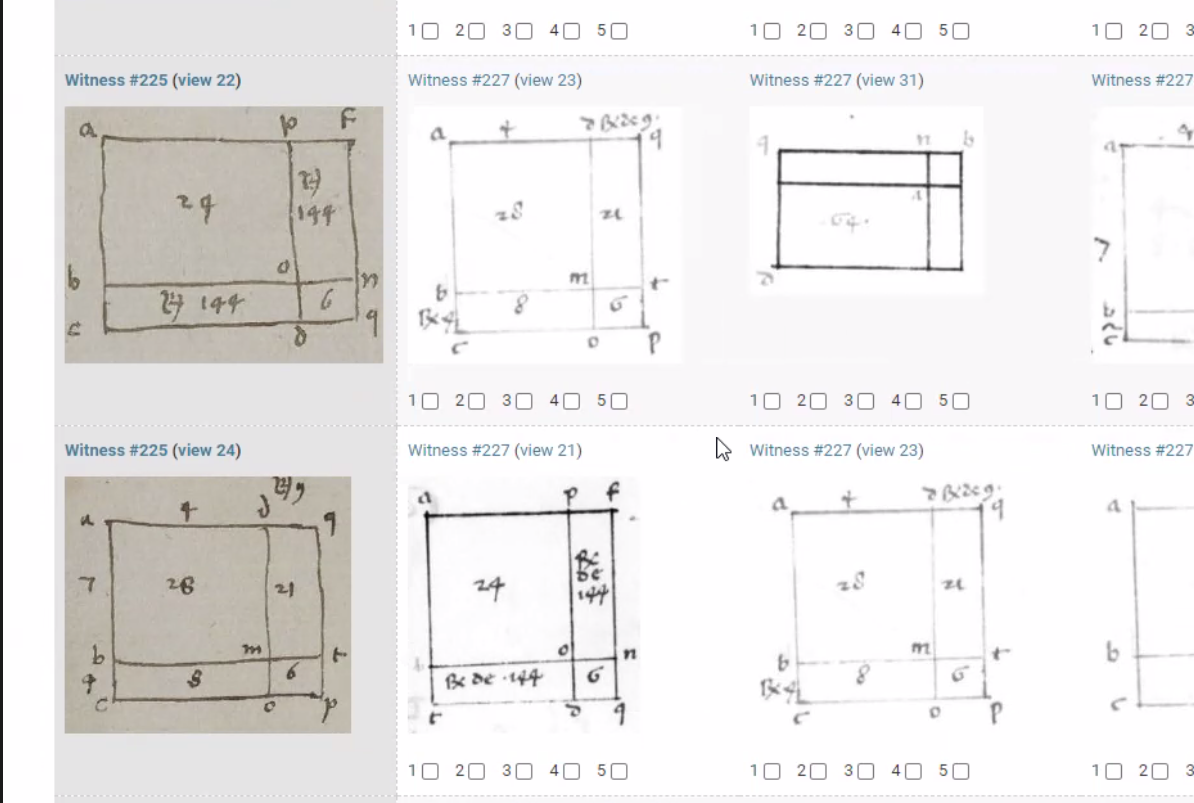
\includegraphics[height=7cm]{figues/label_dissim_exemple.png}
          \end{center}
          \caption{Impact des labels sur la recherche de similarité.}
          \label{fig:simlabel} \end{figure}

Devant ces difficultés il a été décidé d'adopter une annotation binaire
et basée uniquement sur le contenu graphique, partant du principe que
l'assignation d'un score de similarité par le modèle ne vaut pas pour
conclusion historiographique. Il sera toujours plus facile de ne pas
prendre en compte un résultat, et la visée de cet entraînement est
d'aboutir à un modèle assez extensif et généraliste. Il subsiste
cependant des dissensions au sein de l'équipe entre une définition très
stricte de la similarité, quitte à accepter des faux négatifs, et une
définition plus souple (typiquement, sensible aux labels), quitte à
créer des faux positifs. Pour concilier les besoins de tous les
chercheur.ses, il sera recommandé d'annoter selon la définition la plus
rigoureuse d'un point de vue scientifique, cette définition servant de
métadonnée aux chercheur.ses. Les annotations les plus souples seront
utilisées pour l'entraînement du modèle. Cette approche permet de
garantir une précision dans la classification des données tout en
offrant la souplesse nécessaire pour optimiser les performances des
algorithmes d'apprentissage automatique.

Ce cas d'étude est assez caractéristique des enjeux tenant à la
coordination au sein et entre des équipes de recherche dans le cadre du
développement d'un outil commun. D'où le développement des outils
d'annotation dans la plateforme commune assez généralistes pour que leur
usage s'adapte à des besoins différents et complexes\footnote{En
  réalité, les équipes de \vhs sont aussi passées à un classement binaire
  pour prévenir des problèmes de coordination au sein de leurs équipes,
  gardant l'usage des trois autres catégories pour une prochaine étape
  de fine-tuning.}.

\hypertarget{corpus}{%
\subsection{Corpus}\label{corpus}}

Les sources primaires d'\eida couvrent un spectre géographique et
temporel important. Orienté par les objectifs scientifique d'\eida --
arriver à une représentation globale des continuités et divergences qui
se tracent au cœur des pratiques astronomiques à travers l'histoire,
esquisser le voyage des sources à travers le temps et l'espace -- le
refus d'une vision eurocentrée justifie et explique une représentativité
large, servie par la constitution de cinq grands corpus issus de sphères
géographiques et temporelles diverses. Les manuscrits arabo-persans
produits entre le \textsc{viii}\ieme et le \textsc{xiii}\ieme siècle, des manuscrits latins
médiévaux produits majoritairement entre le \textsc{xiii}\ieme et le \textsc{xvi}\ieme siècle, les
manuscrits byzantins, produits entre les \textsc{ix}\ieme et \textsc{xv}\ieme siècles, les
manuscrits sanskrits, à partir du \textsc{xi}\ieme, et enfin les sources chinoises
datant du milieu du \textsc{xvi}\ieme siècle, après l'arrivée des premiers jésuites.
Le support de ces dernières n'est pas nécessairement le manuscrit, elles
prennent souvent la forme d'imprimés par blocs xylographiques dont les
matrices sont réemployées dans plusieurs témoins. Elles présentent donc
une forme hybride, sorte de pré-imprimé, qui posa des questions
complexes pour la modélisation conceptuelle des données.

Plusieurs centaines de manuscrits sont numérisés pour chaque tradition.
Sur ces numérisations, mises à disposition par les institutions
patrimoniales qui conservent ces témoins, seront appliquées les
traitements en prévision de l'analyse par les chercheur.ses, leur
permettant de souligner les motifs qui sous-tendent la diffusion
afro-eurasiens du modèle ptoléméen.

La gémellité avec \vhs impose un effort de modularité pour pouvoir
partager le modèle de données. Le travail de recherche de \vhs est mené
sur quatre corpus relevant, à l'instar de celui d'\eida d'une grande
diversité chronologique et géographique. Ces corpus se distinguent
cependant par une grande diversité thématique~: ils se composent de
manuscrits et d'imprimés concernant les sciences des mathématiques et
les sciences naturelles. Le premier corpus est le \emph{Physiologus},
rédigé vers le \textsc{ii}\ieme siècle à Alexandrie. Ce texte, l'un des plus
populaires du \ma, a contribué à l'émergence de la zoologie
chrétienne médiévale. Il a pour témoins 100 manuscrits grecs, dont treize
sont illustrés et réalisés entre le \textsc{xi}\ieme et le \textsc{xvi}\ieme siècle, contenant
environ 680 images d'animaux, de plantes et de minéraux. Le deuxième
corpus est le \emph{De materia medica} de Dioscoride, composé vers l'an
77 de notre ère. Ce traité pharmacologique destiné aux praticiens a été
largement diffusé et copié. Il est conservé dans 65 manuscrits grecs,
dont 17, réalisés entre le \textsc{vi}\ieme et le \textsc{xvi}\ieme{} siècle, sont illustrés et
contiennent environ 8340 images de plantes, d'animaux et de minéraux.
Les troisième et quatrième corpus se composent des planches de
l'Encyclopédie de Diderot et d'Alembert (1751-1772), les témoins de ce
travail couvrant une longue série de traités, dictionnaires et
encyclopédies au fil desquels les illustrations ont été copiées et
retravaillées. Leur étude se focalise aussi sur leur inclusion
ultérieure dans des encyclopédies telles que l'Encyclopédie méthodique.
Le troisième corpus se concentre sur l'Histoire naturelle (Zoologie),
tandis que le quatrième porte sur les sciences mathématiques\footcite{noauthor_vhs_nodate}.

Le deux corpus jumeaux diffèrent aussi en taille~: celui de \vhs présente plus de 2000 témoins devant 300 pour \eida.

Malgré ces divergences importantes, les données sont issus de spectres
assez larges pour opérer des croisements dont l'exploitation peut
s'avérer fructueuse~: les corpus \vhs présentent quelques diagrammes
astronomiques, et les manuscrits \eida présentent plusieurs images de
plantes. La mise en commun des résultats permet d'établir des liens
entre le \ma (focus d'\eida) et la période moderne (focus de \vhs)
pour les domaines respectifs étudiés. Notamment, des chercheur.ses d'\eida
s'intéressent à la transition du manuscrit à l'imprimé. La possible
jonction des corpus reste néanmoins problématique, et les modèles d'\ia doivent être spécialisés sur les objets d'étude respectifs des deux projets.

Ces remarques sont révélatrices de l'entre-deux qui nous intéresse dans
ce mémoire~: bien que les projets aient un objectif et des objets
d'étude précis, ceux-ci se trouvent élargis par le réseau institutionnel
et les dynamiques collaboratives qui accompagnent la création des outils
numériques. Le niveau de modularité de l'outil créé devra prendre en
compte cette généralisation possible sans perdre de vue les objectifs
initiaux des deux projets.

\hypertarget{modele-de-donnees}{%
\subsection{Modèle de données}\label{modele-de-donnees}}

L'application commune à \vhs/\eida est développée avec le \textit{framework} Django
et adossée sur une base de données gérée avec PostgreSQL. Le modèle de
données conçu pour l'application a fait l'objet de réflexions et
réadaptations pour répondre aux besoins de description des sources de
\vhs et \eida, tout en restant suffisamment flexible pour être utilisé par
d'autres projets souhaitant reproduire les méthodes employées par les
deux projets. Le défi consiste à conceptualiser la donnée de manière
suffisamment spécifique et assez généraliste.

\hypertarget{modele-initial}{%
\subsubsection{Modèle initial}\label{modele-initial}}

Le modèle de données initialement construit\footnote{Voir l'annexe \ref{data_models} pour une illustration de l'évolution du modèle de données.} pour
l'application \vhs prévoit l'existence des entités 'manuscrit' et
'imprimé', qui correspondent aux supports représentés dans
les corpus d'\eida et de \vhs. Ces deux \emph{états matériels} du texte
sont reliés à une entité plus abstraite~: le \wo.
S'appuyant sur la définition de \wo que donne le CIDOC-CRM\footnote{Le
  modèle conceptuel définit, dans un domaine donné, comment représenter
  la réalité. À ce titre il est indépendant de la manière dont on stocke
  les données informatiquement. Né dans le domaine des musées, CIDOC-CRM
  est un modèle conceptuel standardisé pour la modélisation des
  informations dans le domaine du patrimoine. Il vise à décrire et à
  rendre interopérables des objets du monde culturel en général. La
  notion d'événement se trouve au cœur du modèle, traduisant une
  approche monotonique des données~: les objets décrits peuvent évoluer,
  on peut toujours décrire de nouveaux événements liés à cet objet.
  Ainsi, on n'aura potentiellement jamais terminé de décrire un objet en
  CIDOC-CRM.}, un \wo est indépendant de sa forme matérielle, c'est une
production intellectuelle qui peut se manifester dans différentes
sources, pouvant elles-mêmes présenter des variations.

Mais ce premier modèle va rapidement montrer des limites, notamment
liées à la description d'une même œuvre divisée en plusieurs ouvrages,
ou d'un ouvrage contenant plusieurs œuvres. De plus, la pertinence de la
distinction absolue des manuscrits et imprimés ne permet pas une
description pertinente de tous les objets~: par exemple les sources
chinoises, dont le support n'est pas nécessairement le manuscrit,
prennent souvent la forme d'imprimés par blocs xylographiques dont les
matrices sont réemployée. Ces constats ont mené à la refonte de ce
modèle de données. 

\hypertarget{premiere-refonte}{%
\subsubsection{Première refonte}\label{premiere-refonte}}

Le nouveau modèle est non seulement plus pertinent mais aussi déjà plus
flexible. Il est centré autour de l'entité 'témoin' ou \wit, et
est complété par d'autre tables pour décrire la diversité des sources et
leurs différents modes d'existence. Ainsi, les séries héritent
uniquement des imprimés et les témoins héritent à la fois des
manuscrits et des imprimés. Une \ser est une édition en
plusieurs volumes d'une œuvre imprimée. Le témoin ramène à chaque volume
en tant qu'entité matérielle de référence, ou à un manuscrit. Il peut
contenir un ou plusieurs 'travaux' (\wo)~; un même \wo peut
correspondre à des séries et des témoins différents (table de relation
\textit{Content}). La table \wo inclut donc les références au lieu et à l'auteur
(clés étrangères), mais aussi l'information relative à la plage de temps
durant laquelle cette œuvre a existé physiquement (durant laquelle on
atteste l'existence de témoins). La ou les numérisations
(\digits) sont reliées au \wit et contiennent les détails sur la
source de numérisation et l'état des traitements via \iiif\footnote{Voir le \hyperlink{iiif}{Chapitre 2} sur \iiif}. Une entité Tag est utilisée comme moyen de
différencier manuscrit, imprimé ou gravure, et la table de relation
\textit{Tag\_Exemplar} fait le lien entre le témoin et les tags. La table
\textit{Role} établit des relations entre des contenus (\textit{Content}), des
\emph{séries} (\sers) et des personnes (\textit{Persons}), attribuant à
ces dernières les rôles d'auteur ou d'éditeur.

Les évolutions en cours pendant mon stage, détaillées en partie
III\footnote{Voir le \hyperlink{chapitre-7-processus-et-fonctionnalites}{Chapitre 7}}, ont nécessité de faire des choix
complexes, répondant à une double exigence \emph{a priori} paradoxale~:
une plus grande flexibilité pour intégrer de nouvelles sources de
données et une précision de description suffisante. De nouvelles
questions ont été soulevées liées à la granularité et à la cohérence
sémantique.

Ce paradoxe apparent met en lumière les défis et la complexité liés à la
modélisation de la donnée, et les transformations successives reflètent
des questionnements~: comment rendre l'application la plus universelle
possible, l'ouvrir à une large diversité de sources, sans renoncer à la
qualité de la description des sources des projets de \eida et \vhs~?
Comment, d'ailleurs, conceptualiser un modèle qui convienne aux deux
projets et leurs objectifs~? Les solutions ci-dessus décrites sont
satisfaisantes mais amenées à évoluer, montrant que la modularité se
construit sur le temps long.

\vspace{2cm}

En résumé, \eida repose sur la constitution de jeux de données de
diagrammes astronomiques extraits de sources relevant de multiples
domaines linguistiques et culturels, sources connectées à l'échelle
afro-eurasienne. Le projet développe des outils numériques permettant
une approche critique des diagrammes astronomiques à large échelle,
fournissant à ce titre une base solide pour une étude approfondie des
schémas de circulation des connaissances astronomiques entre le
\ma et l'époque moderne.

En \cv, \eida s'appuie sur les récents progrès en
\dl, et teste l'application d'une nouvelle génération de
méthodes vectorisation d'images sur des sources
historiques~: manuscrits, \emph{early prints} et xylogravures.

Au centre de ce projet réside une approche intrinsèquement transversale
et interdisciplinaire, qui s'appuie sur des projets antérieurs et
bénéficie de la collaboration avec des équipes dotées de compétences en
ingénierie, ainsi qu'avec le projet \textsc{anr} \vhs~; bien que les objectifs de
ce dernier divergent de ceux d'\eida. Ainsi, au sein même de l'écosystème
d'un même projet de recherche, les livrables doivent s'adapter aux
usages et besoins des chercheur.ses, à la diversité de leurs questions de
recherche et enfin à deux corpus différents dans toute leur
hétérogénéité. De fait, la problématique de modularisation est au cœur
du projet \vhs/\eida. Cette modularisation impose de créer des composants
logiciels indépendants et réutilisables, facilitant ainsi l'adaptation
du projet aux deux contextes, comme nous le développeront plus avant. En
outre, pour garantir une approche conforme aux principes de l'open-source et de la science ouverte, une couche de standardisation doit être
ajoutée. Cette standardisation vise à rendre les composants du projet
interopérables, permettant ainsi une collaboration transparente et la
réutilisation des résultats de recherche au sein de la communauté
scientifique. En intégrant ces principes dans la conception et le
développement du projet, il devient possible de promouvoir la
transparence, la reproductibilité et l'accessibilité des outils
techniques (modèles de vision) et des corpus enrichis.

            
        \clearemptydoublepage
        
\hypertarget{chapitre-2-open-data-et-enjeux-interop}{%
\chapter{Open-data et enjeux d'interopérabilité~: la standardisation technique à grande échelle}\label{chapitre-2-open-data-et-enjeux-interop}}

                Les acteurs impliqués dans la réalisation d'un outil tel que la
plateforme commune \aikon ne se limitent pas aux participants du projets évoqués
dans la partie précédente. Les potentiels utilisateur.rices futurs et les
institutions détentrices des données sont aussi à prendre en compte,
ils orientent les développements et les fonctionnalités des
outils conçus.

Le traitement des sources iconographiques revêt des enjeux spécifiques
du point de vue technique, juridique et de la disponibilité. La remise
en circulation des résultats des traitements, à l'autre bout de la
chaîne, présente d'autres défis et soulève des questions de visibilité,
d'accès, et de médiation qui sont autant d'exigence à prendre en
considération pour garantir l'utilité des résultats pour l'ensemble des
utilisateur.rices et partenaires impliqués.

Enfin, la mutualisation du code induit des enjeux d'organisation devant aussi être pris en considération.

Ces enjeux contraignent le projet à rentrer dans un cadre technique
rigoureux où plusieurs aspects clés doivent être respectés~:
l'utilisation de standards ouverts pour garantir la compatibilité et
l'interopérabilité entre différents systèmes et outils, l'adoption de
formats de données standardisés pour faciliter le partage et l'échange
d'informations, la conformité avec les réglementations juridiques en
matière de droits d'auteur et de protection des données, et la prise en
compte de l'interaction avec des utilisateur.rices divers.

\begin{kwote}
``une compatibilité technique et sémantique, l'interopérabilité des
données aide au décloisonnement entre domaines d'expertise et permet à
des projets de recherche aux objectifs divergents de s'appuyer sur un
socle commun.''\footcite[p. xvii]{albouy_mediation_2019}
\end{kwote}

                \hypertarget{ouverture-donnees}{%
                \section{Ouverture des données~: accès aux sources et partage des résultats de la recherche}\label{ouverture-donnees}}
                        
L'astronomie est issue d'une tradition continue vieille de près de 4000
ans qui transcende les cultures et les langues. Les théories, les
savoirs, les méthodes, au gré de leur diffusion, se mélangent aux
pratiques autochtones pour servir les usages locaux, qui bien souvent
renforcent des dynamiques de pouvoir en place, que ce dernier soit
politique ou religieux. Les sciences astrales revêtent ainsi une
importance culturelle majeure.

Une étude approfondie des sources révèle les processus par lesquels les
connaissances se sont enrichies et transformées au contact de
différentes cultures. Leur examen permet en outre de souligner les
spécificités et les innovations de chaque tradition, tout en montrant
les interconnexions et les influences réciproques qui ont façonné
l'évolution de l'astronomie. Les schémas de circulation sont dans de
nombreux cas de très grande portée géographique, chronologique et
culturelle. Ils relient des contextes de production de connaissances à
l'échelle afro-eurasienne et sur des périodes de siècles voire de
millénaires. La trace de ces transmission supporte une vision connectée
et globale de l'histoire des cultures et du savoir.

La grande diversité des sources et des approches possibles rend
cependant difficile une approche globale. À ce titre, il est important
de cibler un objet d'étude : \eida se focalise ainsi essentiellement dans
la transmission de la tradition ptoléméenne, et le corpus se compose
donc de ressources manuscrites et imprimées relevant de cette tradition.

\hypertarget{ptolemee-modele-et-transmission}{%
\subsection{Ptolémée : modèle et
transmission}\label{ptolemee-modele-et-transmission}}

Ptolémée tient une place proéminente dans l'histoire de l'astronomie et
des mathématiques. Son nom reste associé à la conception d'un système
astronomique qui plaçait la Terre immobile au centre du monde, et dont
la mise en question, de Copernic à Newton, a commandé la révolution
scientifique.

Dans sa \emph{Syntaxe mathématique}, plus connue sous le titre
d'\emph{Almageste}, et dont la dernière observation consignée date de
141, il expose l'ensemble des connaissances astronomiques de son époque.
Notamment il perfectionne le modèle élaboré par Hipparque, à qui il
emprunte la découverte de l'excentricité des trajectoires apparentes du
Soleil et de la Lune par rapport à la Terre, et l'idée de composer ces
trajectoires à l'aide de deux mouvements distincts. Il élabore un
système géocentrique au moyen d'un ensemble complexe de trajectoires
circulaires des objets pris dans un mouvement uniforme : les déférents,
autour de la Terre, et les épicycles, dont les centres parcourent les
déférents\footcite{lequeux_systeme_nodate}.

En effet, les sociétés anciennes attendent des
corps astraux (soleil, lune, planètes et étoiles) un mouvement uniforme
et le plus ``parfait'' possible, c'est-à-dire un cercle. Pourtant la
trajectoire de ces corps, observée empiriquement, n'est pas circulaire.
Le modèle de Ptolémée explique ces imperfections en postulant que les
mouvement apparemment irréguliers sont dû à cette fameuse combinaison de
plusieurs trajectoires circulaires régulières vues depuis la Terre,
point statique. Les planètes se déplacent à vitesse uniforme sur un
cercle (l'épicycle) dont le centre se déplace à vitesse uniforme sur un
cercle coplanaire (le déférent), dont la Terre est le centre.

En plus de la description du mouvement des astres, Ptolémée dresse dans
l'\emph{Almageste} des tables établissant les positions de la lune et
prévoyant les périodes et les caractéristiques des éclipses avec une
précision inédite\footcite{raymond_jones_ptolemy_2024}, un catalogue des étoiles, un traité
complet de trigonométrie plane et sphérique et une description des
instruments nécessaires à un grand observatoire.

L'œuvre de Ptolémée fera référence, et en tant que synthèse des
connaissances astronomiques antérieures, sa transmission correspond
à celle de la vision des pratiques de l'astronomie grecque à son apogée,
et sa diffusion façonnera la production astronomique ancienne pendant
près de treize siècles. D'ailleurs le nom d'Almageste date de la
transmission par les civilisations arabes à l'occident.

En effet, lors de la chute de l'Empire Romain d'occident, la majeure
partie des ouvrages antiques sont perdus et la science occidentale
stagnera jusqu'au \textsc{xii}\ieme siècle. Elle continuera cependant à progresser
ailleurs : notamment dans le monde arabe et musulman. Dès le \textsc{viii}\ieme et
\textsc{ix}\ieme siècle, les Arabes vont traduire dans leur langue la plupart des
grands textes scientifiques de l'Antiquité, en particulier les œuvres
d'Aristote et l'\emph{Almageste} de Ptolémée. Sans remettre en cause le
géocentrisme et le système de Ptolémée, ils le perfectionnent et
l'amènent à un très grand degré de précision. Nécessaire à la stricte
observation des règles de l'islam, l'astronomie arabe se développe et se
diffuse, grâce aux travaux d'al-Biruni, al-Hazen ou al-Sufi\footcite{noauthor_monde_nodate}.

À partir du \textsc{xi}\ieme et surtout du \textsc{xii}\ieme siècle, au fil des conquêtes des
occidentaux en Espagne et en Sicile, les textes grecques sont traduits
en latin via la traduction arabe. La transmission des savoirs
gréco-arabes -- notamment les traductions arabo-latines de
l'\emph{Almageste} et du Livre des étoiles fixes d'al-Sufi -- ouvre la
voie à un renouveau scientifique dans l'Occident chrétien, permettant
ainsi l'essor des grandes universités européennes de l'époque (Paris,
Oxford, Bologne, etc). On redécouvre les modèles d'Aristote et de
Ptolémée en les adaptant aux conceptions chrétiennes\footcite[``Le
  système géocentrique devient le modèle astronomique et théologique de
  l'Église, qui ne remet pas en cause la sphéricité de la Terre''][]{noauthor_monde_nodate}.

Avant l'avènement de l'astronomie grecque, les Babyloniens, dès le premier
millénaire \jc, utilisaient des calculs arithmétiques pour prévoir
la position des planètes. Ces théories ont voyagé jusqu'en Perse et en
Inde, où elles ont été adaptées et combinées à des méthodes autochtones.
Les théories grecques de l'époque de Ptolémée et de son prédécesseur
Hipparque sont également parvenues jusqu'en Inde, créant un matériel
complexe dont les influences sont difficiles à démêler. Parmi les
pratiques empruntées aux théories grecques, on relève l'emploi de termes
-- par exemple le titre du canon \emph{Romaka Siddhanta} datant du début
du \textsc{v}\ieme et qui marque les origines de la science astronomique sanskrite --
ainsi que des modèles épicycliques et des méthodes de calculs requérant
des paramètres numériques hérités d'Hipparque\footnote{\cite[p.6-7]{mercier_studies_2004} in \cite[p.15]{albouy_mediation_2019}}.

La tradition chinoise se développe de manière relativement indépendante
et les échanges ne débutent qu'autour de 200 \jc. Elle se distingue
de celle des Grecs par un intérêt plus marqué pour la prédiction
d'événements singuliers plutôt que pour les théories cosmologiques
cherchant l'établissement d'un modèle d'organisation du ciel. En effet,
en Chine impériale, l'astronomie a une fonction politique. L'empereur
est considéré comme le Fils du Ciel et ainsi la régulation du
calendrier, ou bien le succès (ou l'échec) de ses astronomes à prédire
une éclipse, se reflétaient positivement ou négativement sur lui.
L'inclusion croissante des diagrammes dans les traités après les
missions jésuites à partir du \textsc{xvi}\ieme siècle révèle l'influence des
pratiques d'Europe de l'ouest.

Pour conclure, l'\emph{Almageste} se présente donc comme une sorte
d'encyclopédie des connaissances d'une époque qui s'est enrichie avec le
temps au point de rendre difficile l'appréciation de son état originel.
Œuvre sans cesse recopiée au cours des siècles, passant du grec à
l'arabe puis au latin, transmise à travers tout le bassin méditerranéen
et dominant le \ma occidental après avoir conquis l'Islām, chaque
traduction et chaque copie de l'Almageste n'ont pas seulement transmis
son contenu, mais l'ont aussi adapté et enrichi en fonction des
contextes culturels et scientifiques de chaque époque. L'œuvre
ptoléméenne a servi de base à de nombreux commentaires et traités,
intégrant progressivement des éléments de connaissance issus de diverses
traditions scientifiques, et illustrant ainsi l'interconnexion des
savoirs à travers les civilisations.

\begin{kwote}
``Certains indices dans les manuscrits révèlent les emprunts
intellectuels qui s'opèrent au fur et à mesure des copies ; les méthodes
de calcul, le tracé des diagrammes, la mise en page des tables, la
structuration des textes techniques, la mention d'auteurs antérieurs, la
réutilisation de paramètres astronomiques ou même la récurrence de
certaines erreurs sont autant de signes qui témoignent des échanges
culturels qui ont façonné la pratique de l'astronomie.''\footcite[p.14]{albouy_mediation_2019}
\end{kwote}

Comme l'entend \citeauthor{albouy_mediation_2019}, les diagrammes font partie des révélateurs des
échanges intellectuels.

\hypertarget{le-diagramme-vecteur-de-connaissances}{%
\subsection{Le diagramme vecteur de
connaissances}\label{le-diagramme-vecteur-de-connaissances}}

L'historiographie et l'histoire des sciences n'échappent pas au récent
``visual digital turn''\footcite[``Digital humanities research has
  focused primarily on the analysis of texts. This emphasis stems from
  the availability of technology to study digitized text. Optical
  character recognition allows researchers to use keywords to search and
  analyze digitized texts. However, archives of digitized sources also
  contain large numbers of images.''][]{wevers_visual_2020} général des
humanités, montrant à quel point la production et la diffusion du savoir
croisent les représentations visuelles rendant compte de ces
connaissance. De fait, on ne s'intéresse plus seulement au texte. Or les
astronomes, au fil de l'histoire, ont eu recours à un grande diversité
de matériaux. Les sources primaires sont constituées par des instruments
et des écrits, ces derniers eux-même hétérogènes. Dans les traités
anciens, on trouve des descriptions détaillées, des propositions
mathématiques, des tables de calcul, et des diagrammes illustrant
souvent le texte qu'ils accompagnent. Les sources primaires peuvent en
outre être enrichies de commentaires et de gloses, prose ou
illustrations, témoignant de la manière dont les connaissances ont été
transmises et interprétées. Elles révèlent également les méthodes
pédagogiques employées pour enseigner ces savoirs.

Au cœur de cette diversité, le diagramme, objet hybride pour deux
raisons : il combine un contenu géométrique (des lignes, arcs et
cercles) et des labels, et il entretient un lien (plus ou moins étroit)
avec le texte qui l'accompagne.

En tant que structure de pensée, la figuration géométrique -- une forme
de création de modèles associée à l'élaboration et à la résolution de
problèmes dans divers domaines de la pensée humaine liés au calcul
abstrait et à la modélisation des idées -- est aussi ancienne que
presque toute autre forme d'enregistrement des pensées et des idées. Des
diagrammes utilisés pour calculer la superficie de parcelles et de
terres apparaissent dans le Papyrus mathématique Rhind, la source la
plus importante qui subsiste pour l'histoire des mathématiques dans
l'Égypte ancienne\footcite[p.6]{safran_diagram_2022}. Instruments
de pensée et de démonstration, ils servent non seulement à transmettre
le savoir mais aussi à le produire. Et dans un étrange mouvement
métaréflexif, ils permettent aux historien.nes des sciences de produire la
connaissance sur ces anciennes traditions heuristiques et leur
transmission.

Les diagrammes sont, pour les astronomes, le support d'une pratique
scientifique, et sont ainsi révélateurs de leurs méthodes, de leur
contexte d'exercice et de leur conception de leur discipline. Ils
revêtent des rôles et des aspects différents, permettant d'identifier
des modes diagrammatiques\footnote{La ``diagrammatisation'' désigne
  assez largement l'investissement des acteurs dans la complexification
  des représentations visuelles des propositions scientifiques présentes
  dans les traités.} spécifiques d'un lieu ou d'une époque, et traçant
des lignes de diffusion des pratiques et des savoirs.

Au \ma, trois grandes cultures coexistent en Eurasie : les
cultures byzantine, islamique, et d'Europe occidentale. Elles
connaissent des évolutions différentes en termes linguistiques et
religieux ; cette diversité est vraie également pour les usages auxquels
les diagrammes astronomiques étaient destinés, pour les domaines dans
lesquels ils étaient reconnus comme des instruments de pédagogie et des
vecteurs de pensée, ainsi que pour la place accordée à la culture
visuelle plus généralement et aux modes de représentation
diagrammatiques. Pourtant cette coexistence donne lieu à des échanges
intellectuels, artistiques, diplomatiques et commerciaux. Les
traductions d'œuvres savantes, les transferts de manuscrits illustrent
la porosité des frontières du savoir et de l'interdépendance des
cultures. Les diagrammes astronomiques sont à ce titre témoins des
chemins de diffusion des connaissance et des pratiques des sciences.

\emph{Comment ces diagrammes parlent-ils aux historien.nes ?}

Les diagrammes peuvent être étudiés intrinsèquement (quelles conventions
gouvernaient le langage visuel, quelle fonction assumaient-ils ?) ou
extrinsèquement (pour comprendre la transmission de ces traditions et
ces pratiques entre l'Europe et l'Asie, en passant pas la péninsule
arabique).

On pourrait penser que les formes et éléments visuels
utilisés pour une démonstration géométrique soient universels, qu'ils
restent les mêmes quelle que soit la date et la langue de l'explication
textuelle, le grec, l'arabe ou le latin\ldots{} Et pourtant le contexte
géographique, temporel, et les aspects matériels liés aux technologies
d'inscription changent profondément le fonctionnement et les objectifs des diagrammes,
leurs objectifs.

L'évolution des conventions graphiques en sont un exemple frappant. Par
exemple, l'axe vertical de la Terre, bien que représenté à plat sur la
page, fut conventionnellement compris comme un axe perpendiculaire à la
coupe du globe. Au fil du temps, de nouvelles conventions graphiques ont
été adoptées, et pour les lecteurs d'aujourd'hui on représenterait
sûrement le globe terrestre avec sa profondeur pour expliciter la
représentation. Citons en outre la représentation des phases lunaires,
qui a connu une évolution concernant l'association des couleurs claire
et sombre à la pleine lune et à la nouvelle lune. Si aujourd'hui on
associerait plutôt la pleine lune à un aplat de couleur claire et la
nouvelle lune à une couleur sombre, les manuscrits médiévaux byzantins
adoptent le référentiel contraire.

De même, le rôle du diagrammes est fluctuant, et va au delà du simple
support démonstratif au service du texte. Par exemple ceux des
\emph{Traités logiques} d'Aristote ont probablement circulé
indépendamment du texte, même si tout indique que les écrits les
appelaient dès le départ. Cela souligne la distinction entre le
diagramme en tant qu'objet de démonstration et de discussion complétant
une proposition d'un côté, et le diagramme en tant qu'accompagnement des
textes scolaires, qui aide à la compréhension de l'autre\footcite[p.5]{safran_diagram_2022}. Le
diagramme peut ainsi constituer la preuve et le support d'une
réinterprétation de la proposition textuelle.

Par-dessus tout, les transformations subies au fil des copies et des
réceptions sont éloquentes pour les chercheurs. Bien que les diagrammes
soient initialement conçus pour clarifier et expliquer une proposition textuelle, ils peuvent
parfois être des vecteurs de confusion (ou d'innovation). Le même diagramme d'une même
œuvre soumis à un processus constant de transformation par les scribes,
les artistes ou les lecteurs/commentateurs. 

La recherche des erreurs
transmises a ainsi un intérêt philologique important. Les cas de
méprises et les malentendus sont peut-être plus nombreux que les cas de
compréhension fidèle lors de la traversée des frontières géographiques,
culturelles, religieuses et/ou linguistiques, et l'étude des erreurs et modifications
révèle leurs aspects heuristiques, autant qu'il peut amener à
l'établissement d'un stemma\footcite{raynaud_building_2014}.

L'importance des diagrammes dans les transmissions est illustrée par l'exemple des diagrammes attribués à al-Ḥajjāj, en lien avec la transmission arabe des \emph{Éléments} d'Euclide. Bien que la traduction originale d'al-Ḥajjāj soit perdue, les diagrammes retrouvés dans divers manuscrits montrent qu'il utilisait parfois des schémas différents de ceux adoptés dans la tradition arabe ultérieure. Ces diagrammes ont probablement joué un rôle clé dans l'élaboration d'une version alternative de la géométrie euclidienne, influençant ainsi la transmission vers l'Europe via les traductions latines et hébraïques\footcite{de_young_editing_2014}.

Ainsi, au travers des variations, similarités et évolutions des
diagrammes, les historien.nes peuvent reconstruire les pratiques
scientifiques des astronomes et comprendre les contextes culturels et
sociaux dans lesquels elles s'inscrivaient. De telles études permettent
aussi de tracer la circulation des sources dans le monde entre les
différentes cultures et de comprendre comment celle-ci s'approprient le
contenu. En somme, l'évaluation de phénomènes diagrammatiques
indéniablement disparates à travers des géographies éloignées permet
d'identifier des modalités d'échanges culturels et leur impact sur la
construction du savoir scientifique.

Les travaux antérieurs sur l'illustration scientifique se concentrent
essentiellement sur des types spécifiques de diagrammes, situés dans des
contextes déterminés chronologiquement et culturellement. Un exemple de
ce paradigme est le projet précédent ALFA, qui porte sur les diagrammes
de tradition alfonsine médiévaux un regard eurocentré. Cependant, à
l'aune des remarques précédentes, il devient pressant de dépasser cette
perspective centripète en étendant la portée géographique et temporelle
des projets ; ambition rendue possible par la disponibilité des sources
primaires en ligne, permettant la construction de bases de données
d'images de grande envergure. Ainsi peut être mise en œuvre une analyse
plus inclusive et diversifiée des sources iconographiques -- notamment
les diagrammes\footcite{husson_eida_2022}.

Comme le dit Jeffrey F. Hamburger dans un plaidoyer pour une étude
comparative des diagrammes astronomique : ``Diagrames can thus be seen
not as embodiements of eternal truths, but, rather, as culturally
embedded objects''\footcite[p.7]{safran_diagram_2022}.

\begin{kwote}
``(\ldots) to be effective, a cross-cultural comparison of diagrammatic
traditions must look beyond the prima facies appearence of the diagrams
under consideration to their underlying operations and the patterns of
thoughts that they both codified and were intended to
inculcate.''\footcite[p.3]{safran_diagram_2022}
\end{kwote}         

Les interrogations soulevées par le projet \eida se déclinent donc comme
suit : analyser l'articulation entre les fonctions documentaires et
épistémiques des diagrammes au sein de l'histoire des pratiques
astronomiques, interroger l'importance des diagrammes dans la
construction et la transmission des connaissances scientifiques, et
enfin identifier des schémas récurrents dans les modalités de
circulation de ces diagrammes. S'appuyant sur ces analyses, les
chercheurs pourront à leur tour tracer des lignes : au sens figuré
construire ``a web of connections linking the points represented by the
individual contributions together into a larger pattern''\footcite[p.10]{safran_diagram_2022} ; et
au sens propre, cette vision globale sur la vie des images et des œuvres
pouvant permettre l'établissement d'éditions critiques normalisées.
            
                \hypertarget{iiif}{%
                \section{IIIF}\label{iiif}}
                        \gaga mène une réflexion
méthodologique sur la portabilité des modèles, leur diffusion et le
partage de grands ensembles de données annotées selon des normes
communes. Les modèles d'\ia, notamment ceux dédiés à la
reconnaissance du texte manuscrit (\htr) et au traitement automatique des
langues (\tal), requièrent des données d'entraînement spécifiques. 

Mais si chaque projet de recherche annotait ses corpus selon ses propres
exigences, ils engendreraient fatalement des silos de données non
réutilisables. Pour garantir la réutilisation des données, il est
impératif d'établir des normes et des standards.

Le projet porte alors le développement d'une syntaxe
d'annotation générique pour harmoniser la segmentation des pages des
vérités de terrain, afin de constituer des corpus d'entraînement réutilisables. \gaga propose une
approche très inclusive en identifiant des éléments textuels communs à
une large variété de documents, manuscrits comme imprimés. Cette
démarche donne lieu à la définition d'un vocabulaire contrôlé permettant
ainsi de construire des corpus annotés compatibles avec différents contextes\footcite[``Using a common vocabulary to annotate zones called SegmOnto (that is still evolving), we have developed a generic workflow to analyse the layout, OCRise the text, and convert the ALTO output into minimally encoded TEI files (\dots).''][p.2]{janes_towards_2021}~:
SegmOnto\footnote{https://github.com/SegmOnto}

Les étapes de lemmatisation et d'étiquetage morphologique (POS-tagging) effectuées par les modèles de \tal sur le texte extrait des pages numérisées visent à normaliser le
langage en réduisant les mots à leur forme canonique (lemme) et en
identifiant leur catégorie grammaticale. Cette normalisation est
essentielle pour faciliter des analyses ultérieures telles que la
collation et la stylométrie. Elle permet une analyse comparative des textes
malgré la grande variabilité inhérentes aux
langues historiques, pour lesquelles l'absence de normes orthographiques entraîne une
grande diversité de graphies. La préparation des données, là aussi, a donné lieu à une
réflexion méthodologique sur les défis liés à la standardisation des
annotations linguistiques dans les corpus diachroniques.

Selon \citeauthor{gabay_standardizing_2020}~:
\begin{kwote}                     
	``With the development of big corpora of various periods, it becomes
	crucial to standardise linguistic annotation (e.g.~lemmas, POS tags,
	morphological annotation) to increase the interoperability of the data
	produced, despite diachronic variations.''\footcite[p.2]{gabay_standardizing_2020}
\end{kwote}  

\citeauthor{gabay_standardizing_2020}\footcite{gabay_standardizing_2020} relèvent la
difficulté de mettre en œuvre un cadre technique qui prenne en compte
les pratiques d'annotation déjà établies et propres à des états de la langue. Pourtant garantir une
interopérabilité minimale avec les corpus existants est essentielle pour
maximiser la valeur ajoutée des nouvelles données.

\begin{kwote}                     
	``Such a task cannot be done without taking into account longstanding
	annotation practices, in order to allow (minimal) interoperability with
	already existing datasets. Such a statement is sadly easier said than
	done, because EMF is an intermediary stage between medieval (12th-15th
	c.) and late modern and contemporary (from c.~1750) French, two states
	of language that tend to have different needs regarding annotation: EMF
	is then caught in between two (potentially incompatible) practices, one
	for each extreme of the continuum.''\footcite[p.2]{gabay_standardizing_2020}
\end{kwote}     

Il est particulièrement complexe de trouver un équilibre entre une
description linguistique trop fine, qui pourrait limiter
la réutilisabilité des corpus, et une description trop générale, qui pourrait
manquer de précision. De plus, les besoins en annotation varient considérablement
entre le français médiéval et le français moderne, et les systèmes
d'annotation de ses deux états de la langue sont difficilement
réconciliables~: or une large partie des sources de \gaga se
situent dans l'entre-deux. Trouver un compromis qui satisfait les
exigences spécifiques de chaque période est complexe.

L'harmonisation des annotations vise à favoriser la diffusion des corpus
de données sur HTR-United, une plateforme collaborative dédiée au
catalogage de vérités de terrain pour l'\htr et l'\ocr, principalement en
français\footcite{chague_htr-united_2021}. Cette base de
données, hébergée sur GitHub, centralise des images et leurs
transcriptions produites par différents projets de recherche, offrant
ainsi une diversité de jeux de données diachroniques et géographiques
pour l'entraînement de modèles \htr.

\gaga vise aussi à la diffusion des modèles en eux-même, qui peuvent alors être réutilisés et spécialisés. Par ailleurs, le projet
s'appuie sur des outils existants, par exemple Deucalion, une boîte à
outils de traitement automatique des langues (\tal) conçue pour être
interopérable avec d'autres systèmes\footnote{https://github.com/chartes/deucalion-model-af}.

\vspace{2cm}

Donc si les stratégies d'accès à la donnée se voudraient universelles,
il existe des limitations techniques ou juridiques demandant une
flexibilité dans les modes d'accès aux sources. Il faut donc laisser
ouvert des modes d'accès plus ``artisanaux'' (fichiers stockés en local,
métadonnées rentrées manuellement) que le standard \iiif, mais aussi
garantir une gestion des droits d'accès aux sources et leur
exploitation, afin de respecter les exigences des
institutions détentrices. 


            
        \clearemptydoublepage
        
\hypertarget{chapitre-3-EDA-image-ia}{%
\chapter{État de l'art~: IA et traitement du volume}\label{chapitre-3-EDA-image-ia}}

            La \bnf constate le besoin d'automatisation pour traiter les volumétries
croissantes des collections numérisées, en outre caractérisées par une
variété considérable, et elle relève les tensions se jouant dans le traitement en
masse de données hétérogènes.

\begin{kwote}

"De plus en plus confrontées à des niveaux de volumétrie et de vélocité
typiques des mégadonnées (big data), les collections numériques de la
\bnf, qui occupent aujourd'hui environ six pétaoctets, sont caractérisées
par une variété considérable. Documents numérisés, tels que par exemple
les livres et manuscrits consultables dans Gallica --- la bibliothèque
numérique de la \bnf ---~; documents nativement numériques comme les
œuvres d'art vidéo, les logiciels, les bases de données, les archives de
l'Internet~; métadonnées bibliographiques et données d'autorité
décrivant les personnes, lieux, organisations, concepts\ldots{} autant
d'ensembles de données diverses en termes de structures, formats,
qualité, contextes de production, fonctions et contenus. Ces ensembles
ont des histoires différentes, issues des changements des supports et
des multiples strates de pratiques documentaires accumulées au fil du
temps. Leur hétérogénéité exige des traitements spécifiques et par
conséquent des compétences et des méthodes particulières, aussi bien
pour les conserver ou les communiquer que pour les analyser (cf
Moiraghi, 2017). Cette hétérogénéité des données, qui découle de
l'amplitude chronologique et de la vocation à l'encyclopédisme
caractéristiques des bibliothèques nationales, s'ajoute à
l'accroissement de la quantité des données en entrée et à l'accélération
conséquente des temps de traitement. La tendance traditionnelle des
bibliothèques à la systématisation des procédures doit dès lors trouver
son équilibre face à la spécificité des données mais aussi des questions
scientifiques propres aux projets de recherche qui les
exploitent".\footcite[p.6]{bermes_patrimoine_2020}  
\end{kwote}

L'état de l'art montre une convergence vers l'utilisation de
l'intelligence artificielle pour traiter efficacement des corpus de
données de plus en plus vastes et complexes. Cette systématisation doit
cependant être équilibrée par une compréhension fine des contextes
locaux et spécifiques des données, afin de garantir la pertinence et
l'efficacité des outils développés.

Les explorations autour du traitement du patrimoine numérique menées à
la \bnf\footnote{\cite{bermes_patrimoine_2020}, \cite{beaudouin_cartographie_2017}, \cite{michez_gallicapix_2021}, \cite{bouchard_presentation_2017}},
en rapport étroit avec des projets de recherche en \hn, illustrent bien
cette tension. Ces projets ont porté sur des ensembles de données
balisés et spécifiques (tel que les sources documentaires numérisées
autour de la guerre 14-18, les publicités de 1910 à 1920, illustrations
du magazine de mode Vogue de 1920 à 1940 ou encore illustrations de
papier peint\footnote{\cite{beaudouin_cartographie_2017}, \cite{michez_gallicapix_2021}}). L'absence de
passage à l'échelle est significatif des difficultés d'un traitement et
d'un enrichissement systématique et standardisé de très grands volumes de données très
hétérogènes. Ainsi, chacun des projets reposait sur des méthodes et des
techniques différentes en raison de la nature des données explorées et
des finalités scientifiques propres à chaque projet.

Cependant des leçons ont été tirées~: les résultats découlent d'un
travail collectif et interdisciplinaire, et se sont appuyés sur des
méthodes standardisées, par exemple pour l'extraction des données et
métadonnées via des \apis\footcite[p.7]{bermes_patrimoine_2020}. Ces
premières applications de l'\ia ont démontré la nécessite de garantir la
reproductibilité des méthodes et d'adopter des normes pouvant mettre en
œuvre un cadre technique interopérable afin de faciliter la
collaboration à plusieurs échelles~: entre les projets de recherche d'un
part, et d'autre part entre les disciplines et les corps de métier
(notamment entre les chercheur.ses et les professionnels des
bibliothèques).

Le projet \gaga\footnote{https://gallicorpora.github.io/} --
bénéficiant de l'appui du DataLab de la \bnf -- se détache néanmoins dans
le paysage des projets estampillés \bnf, car il aspire à s'éloigner le
plus possible de son corpus, voulant concilier reproductibilité des
résultats sur des données diverses et applicabilité à un large corpus
issu des collections numérisées de la Bibliothèque Nationale. Il
illustre en outre les problématiques susmentionnées~: l'inscription dans
un dialogue interdisciplinaire et dans des pratiques normalisées.
L'ambition du projet porte sur le développement d'une chaîne de
traitement automatisée pour la transcription et l'annotation des documents textuels historiques, en diachronie longue, en
partant de leurs numérisations disponibles sur le portail Gallica,
créant ainsi des corpus enrichis, et facilitant leur exploitation et
leur valorisation. En effet les besoins des institution se déplacent de la transcription des textes à leur encodage sémantique automatique en \xml-\tei, afin d'offrir
utilisateur.rices de bibliothèques numériques de nouvelles options pour la
fouille de données. Le projet \gaga s'inscrit dans cette
dynamique, en exploitant le riche corpus de la \bnf, qui met à disposition 193 265
manuscrits, dont 52 188 précédent 1800, et 1 182 471 livres imprimés,
dont 160 335 précédent 1800\footcite{sagot_gallicorpor_2022}.

\begin{kwote}  
``Le nouveau défi à relever aujourd'hui est de transformer ces
numérisations en des ressources enrichies, qui augmentent le texte
extrait et repérable avec de la métadonnée et de l'analyse. Le texte
brut et non annoté ne suffit plus pour la recherche en informatique
appliquée aux documents historiques. De là vient l'impulsion pour le
projet \gaga. Le projet envisage la mise en place d'un pipeline
qui saisit un document numérisé depuis le portail Gallica et renvoie une
ressource numérique très enrichie. En plus d'une description du texte
repérable, la ressource présentera les données structurelles portant sur
la mise en page, ainsi qu'une analyse linguistique du texte extrait et
des métadonnées portant sur le document physique et le fac-similé
numérique''.\footcite{christensen_gallicorpor_2022}.
\end{kwote}

En outre, le but sous-jacent du projet est de produire un prototype qui
pourrait servir d'exemple de chaîne d'acquisition
numérique pour les institutions
patrimoniales. Par conséquent, ce projet se propose aussi d'être une
preuve de concept d'un \emph{modus operandi} pour l'extraction et
l'annotation de textes très divers, créant une sorte de pipeline ultime. Mais avant tout, la chaîne de traitement est destinée à être applicable
à un large corpus de documents mis à disposition par la \bnf. Les
documents du corpus visé proviennent de différentes époques (du \textsc{xv}\ieme au
\textsc{xviii}\ieme siècle) et présentent une grande diversité de mises en page, de
langues (ancien français, moyen français, français classique), et de
supports (manuscrits, imprimés). L'hétérogénéité des sources est censée
faire preuve de faisabilité, et vérifier le potentiel de la méthode
élaborée. Elle vise à prouver que le concept d'une chaîne de traitement
généraliste peut être concrètement appliquée.

\gaga expose ainsi la plupart des questionnements et défis
tenant au montage d'une chaîne de traitement unifiée applicable à une
grande diversité de données. Les choix technologiques, tels que
l'adoption de formats ouverts et interopérables, la prise en compte de
la diversité des modes d'acquisition des données et la spécialisation
des modèles d'\ia, sont au cœur de ces enjeux. Par ailleurs, la question
de l'ouverture des corpus annotés, essentielle pour l'apprentissage
machine, est également un axe d'analyse à considérer.

                \hypertarget{formats-standards}{\section{%
                Formats standards}\label{formats-standards}}
                    
L'astronomie est issue d'une tradition continue vieille de près de 4000
ans qui transcende les cultures et les langues. Les théories, les
savoirs, les méthodes, au gré de leur diffusion, se mélangent aux
pratiques autochtones pour servir les usages locaux, qui bien souvent
renforcent des dynamiques de pouvoir en place, que ce dernier soit
politique ou religieux. Les sciences astrales revêtent ainsi une
importance culturelle majeure.

Une étude approfondie des sources révèle les processus par lesquels les
connaissances se sont enrichies et transformées au contact de
différentes cultures. Leur examen permet en outre de souligner les
spécificités et les innovations de chaque tradition, tout en montrant
les interconnexions et les influences réciproques qui ont façonné
l'évolution de l'astronomie. Les schémas de circulation sont dans de
nombreux cas de très grande portée géographique, chronologique et
culturelle. Ils relient des contextes de production de connaissances à
l'échelle afro-eurasienne et sur des périodes de siècles voire de
millénaires. La trace de ces transmission supporte une vision connectée
et globale de l'histoire des cultures et du savoir.

La grande diversité des sources et des approches possibles rend
cependant difficile une approche globale. À ce titre, il est important
de cibler un objet d'étude : \eida se focalise ainsi essentiellement dans
la transmission de la tradition ptoléméenne, et le corpus se compose
donc de ressources manuscrites et imprimées relevant de cette tradition.

\hypertarget{ptolemee-modele-et-transmission}{%
\subsection{Ptolémée : modèle et
transmission}\label{ptolemee-modele-et-transmission}}

Ptolémée tient une place proéminente dans l'histoire de l'astronomie et
des mathématiques. Son nom reste associé à la conception d'un système
astronomique qui plaçait la Terre immobile au centre du monde, et dont
la mise en question, de Copernic à Newton, a commandé la révolution
scientifique.

Dans sa \emph{Syntaxe mathématique}, plus connue sous le titre
d'\emph{Almageste}, et dont la dernière observation consignée date de
141, il expose l'ensemble des connaissances astronomiques de son époque.
Notamment il perfectionne le modèle élaboré par Hipparque, à qui il
emprunte la découverte de l'excentricité des trajectoires apparentes du
Soleil et de la Lune par rapport à la Terre, et l'idée de composer ces
trajectoires à l'aide de deux mouvements distincts. Il élabore un
système géocentrique au moyen d'un ensemble complexe de trajectoires
circulaires des objets pris dans un mouvement uniforme : les déférents,
autour de la Terre, et les épicycles, dont les centres parcourent les
déférents\footcite{lequeux_systeme_nodate}.

En effet, les sociétés anciennes attendent des
corps astraux (soleil, lune, planètes et étoiles) un mouvement uniforme
et le plus ``parfait'' possible, c'est-à-dire un cercle. Pourtant la
trajectoire de ces corps, observée empiriquement, n'est pas circulaire.
Le modèle de Ptolémée explique ces imperfections en postulant que les
mouvement apparemment irréguliers sont dû à cette fameuse combinaison de
plusieurs trajectoires circulaires régulières vues depuis la Terre,
point statique. Les planètes se déplacent à vitesse uniforme sur un
cercle (l'épicycle) dont le centre se déplace à vitesse uniforme sur un
cercle coplanaire (le déférent), dont la Terre est le centre.

En plus de la description du mouvement des astres, Ptolémée dresse dans
l'\emph{Almageste} des tables établissant les positions de la lune et
prévoyant les périodes et les caractéristiques des éclipses avec une
précision inédite\footcite{raymond_jones_ptolemy_2024}, un catalogue des étoiles, un traité
complet de trigonométrie plane et sphérique et une description des
instruments nécessaires à un grand observatoire.

L'œuvre de Ptolémée fera référence, et en tant que synthèse des
connaissances astronomiques antérieures, sa transmission correspond
à celle de la vision des pratiques de l'astronomie grecque à son apogée,
et sa diffusion façonnera la production astronomique ancienne pendant
près de treize siècles. D'ailleurs le nom d'Almageste date de la
transmission par les civilisations arabes à l'occident.

En effet, lors de la chute de l'Empire Romain d'occident, la majeure
partie des ouvrages antiques sont perdus et la science occidentale
stagnera jusqu'au \textsc{xii}\ieme siècle. Elle continuera cependant à progresser
ailleurs : notamment dans le monde arabe et musulman. Dès le \textsc{viii}\ieme et
\textsc{ix}\ieme siècle, les Arabes vont traduire dans leur langue la plupart des
grands textes scientifiques de l'Antiquité, en particulier les œuvres
d'Aristote et l'\emph{Almageste} de Ptolémée. Sans remettre en cause le
géocentrisme et le système de Ptolémée, ils le perfectionnent et
l'amènent à un très grand degré de précision. Nécessaire à la stricte
observation des règles de l'islam, l'astronomie arabe se développe et se
diffuse, grâce aux travaux d'al-Biruni, al-Hazen ou al-Sufi\footcite{noauthor_monde_nodate}.

À partir du \textsc{xi}\ieme et surtout du \textsc{xii}\ieme siècle, au fil des conquêtes des
occidentaux en Espagne et en Sicile, les textes grecques sont traduits
en latin via la traduction arabe. La transmission des savoirs
gréco-arabes -- notamment les traductions arabo-latines de
l'\emph{Almageste} et du Livre des étoiles fixes d'al-Sufi -- ouvre la
voie à un renouveau scientifique dans l'Occident chrétien, permettant
ainsi l'essor des grandes universités européennes de l'époque (Paris,
Oxford, Bologne, etc). On redécouvre les modèles d'Aristote et de
Ptolémée en les adaptant aux conceptions chrétiennes\footcite[``Le
  système géocentrique devient le modèle astronomique et théologique de
  l'Église, qui ne remet pas en cause la sphéricité de la Terre''][]{noauthor_monde_nodate}.

Avant l'avènement de l'astronomie grecque, les Babyloniens, dès le premier
millénaire \jc, utilisaient des calculs arithmétiques pour prévoir
la position des planètes. Ces théories ont voyagé jusqu'en Perse et en
Inde, où elles ont été adaptées et combinées à des méthodes autochtones.
Les théories grecques de l'époque de Ptolémée et de son prédécesseur
Hipparque sont également parvenues jusqu'en Inde, créant un matériel
complexe dont les influences sont difficiles à démêler. Parmi les
pratiques empruntées aux théories grecques, on relève l'emploi de termes
-- par exemple le titre du canon \emph{Romaka Siddhanta} datant du début
du \textsc{v}\ieme et qui marque les origines de la science astronomique sanskrite --
ainsi que des modèles épicycliques et des méthodes de calculs requérant
des paramètres numériques hérités d'Hipparque\footnote{\cite[p.6-7]{mercier_studies_2004} in \cite[p.15]{albouy_mediation_2019}}.

La tradition chinoise se développe de manière relativement indépendante
et les échanges ne débutent qu'autour de 200 \jc. Elle se distingue
de celle des Grecs par un intérêt plus marqué pour la prédiction
d'événements singuliers plutôt que pour les théories cosmologiques
cherchant l'établissement d'un modèle d'organisation du ciel. En effet,
en Chine impériale, l'astronomie a une fonction politique. L'empereur
est considéré comme le Fils du Ciel et ainsi la régulation du
calendrier, ou bien le succès (ou l'échec) de ses astronomes à prédire
une éclipse, se reflétaient positivement ou négativement sur lui.
L'inclusion croissante des diagrammes dans les traités après les
missions jésuites à partir du \textsc{xvi}\ieme siècle révèle l'influence des
pratiques d'Europe de l'ouest.

Pour conclure, l'\emph{Almageste} se présente donc comme une sorte
d'encyclopédie des connaissances d'une époque qui s'est enrichie avec le
temps au point de rendre difficile l'appréciation de son état originel.
Œuvre sans cesse recopiée au cours des siècles, passant du grec à
l'arabe puis au latin, transmise à travers tout le bassin méditerranéen
et dominant le \ma occidental après avoir conquis l'Islām, chaque
traduction et chaque copie de l'Almageste n'ont pas seulement transmis
son contenu, mais l'ont aussi adapté et enrichi en fonction des
contextes culturels et scientifiques de chaque époque. L'œuvre
ptoléméenne a servi de base à de nombreux commentaires et traités,
intégrant progressivement des éléments de connaissance issus de diverses
traditions scientifiques, et illustrant ainsi l'interconnexion des
savoirs à travers les civilisations.

\begin{kwote}
``Certains indices dans les manuscrits révèlent les emprunts
intellectuels qui s'opèrent au fur et à mesure des copies ; les méthodes
de calcul, le tracé des diagrammes, la mise en page des tables, la
structuration des textes techniques, la mention d'auteurs antérieurs, la
réutilisation de paramètres astronomiques ou même la récurrence de
certaines erreurs sont autant de signes qui témoignent des échanges
culturels qui ont façonné la pratique de l'astronomie.''\footcite[p.14]{albouy_mediation_2019}
\end{kwote}

Comme l'entend \citeauthor{albouy_mediation_2019}, les diagrammes font partie des révélateurs des
échanges intellectuels.

\hypertarget{le-diagramme-vecteur-de-connaissances}{%
\subsection{Le diagramme vecteur de
connaissances}\label{le-diagramme-vecteur-de-connaissances}}

L'historiographie et l'histoire des sciences n'échappent pas au récent
``visual digital turn''\footcite[``Digital humanities research has
  focused primarily on the analysis of texts. This emphasis stems from
  the availability of technology to study digitized text. Optical
  character recognition allows researchers to use keywords to search and
  analyze digitized texts. However, archives of digitized sources also
  contain large numbers of images.''][]{wevers_visual_2020} général des
humanités, montrant à quel point la production et la diffusion du savoir
croisent les représentations visuelles rendant compte de ces
connaissance. De fait, on ne s'intéresse plus seulement au texte. Or les
astronomes, au fil de l'histoire, ont eu recours à un grande diversité
de matériaux. Les sources primaires sont constituées par des instruments
et des écrits, ces derniers eux-même hétérogènes. Dans les traités
anciens, on trouve des descriptions détaillées, des propositions
mathématiques, des tables de calcul, et des diagrammes illustrant
souvent le texte qu'ils accompagnent. Les sources primaires peuvent en
outre être enrichies de commentaires et de gloses, prose ou
illustrations, témoignant de la manière dont les connaissances ont été
transmises et interprétées. Elles révèlent également les méthodes
pédagogiques employées pour enseigner ces savoirs.

Au cœur de cette diversité, le diagramme, objet hybride pour deux
raisons : il combine un contenu géométrique (des lignes, arcs et
cercles) et des labels, et il entretient un lien (plus ou moins étroit)
avec le texte qui l'accompagne.

En tant que structure de pensée, la figuration géométrique -- une forme
de création de modèles associée à l'élaboration et à la résolution de
problèmes dans divers domaines de la pensée humaine liés au calcul
abstrait et à la modélisation des idées -- est aussi ancienne que
presque toute autre forme d'enregistrement des pensées et des idées. Des
diagrammes utilisés pour calculer la superficie de parcelles et de
terres apparaissent dans le Papyrus mathématique Rhind, la source la
plus importante qui subsiste pour l'histoire des mathématiques dans
l'Égypte ancienne\footcite[p.6]{safran_diagram_2022}. Instruments
de pensée et de démonstration, ils servent non seulement à transmettre
le savoir mais aussi à le produire. Et dans un étrange mouvement
métaréflexif, ils permettent aux historien.nes des sciences de produire la
connaissance sur ces anciennes traditions heuristiques et leur
transmission.

Les diagrammes sont, pour les astronomes, le support d'une pratique
scientifique, et sont ainsi révélateurs de leurs méthodes, de leur
contexte d'exercice et de leur conception de leur discipline. Ils
revêtent des rôles et des aspects différents, permettant d'identifier
des modes diagrammatiques\footnote{La ``diagrammatisation'' désigne
  assez largement l'investissement des acteurs dans la complexification
  des représentations visuelles des propositions scientifiques présentes
  dans les traités.} spécifiques d'un lieu ou d'une époque, et traçant
des lignes de diffusion des pratiques et des savoirs.

Au \ma, trois grandes cultures coexistent en Eurasie : les
cultures byzantine, islamique, et d'Europe occidentale. Elles
connaissent des évolutions différentes en termes linguistiques et
religieux ; cette diversité est vraie également pour les usages auxquels
les diagrammes astronomiques étaient destinés, pour les domaines dans
lesquels ils étaient reconnus comme des instruments de pédagogie et des
vecteurs de pensée, ainsi que pour la place accordée à la culture
visuelle plus généralement et aux modes de représentation
diagrammatiques. Pourtant cette coexistence donne lieu à des échanges
intellectuels, artistiques, diplomatiques et commerciaux. Les
traductions d'œuvres savantes, les transferts de manuscrits illustrent
la porosité des frontières du savoir et de l'interdépendance des
cultures. Les diagrammes astronomiques sont à ce titre témoins des
chemins de diffusion des connaissance et des pratiques des sciences.

\emph{Comment ces diagrammes parlent-ils aux historien.nes ?}

Les diagrammes peuvent être étudiés intrinsèquement (quelles conventions
gouvernaient le langage visuel, quelle fonction assumaient-ils ?) ou
extrinsèquement (pour comprendre la transmission de ces traditions et
ces pratiques entre l'Europe et l'Asie, en passant pas la péninsule
arabique).

On pourrait penser que les formes et éléments visuels
utilisés pour une démonstration géométrique soient universels, qu'ils
restent les mêmes quelle que soit la date et la langue de l'explication
textuelle, le grec, l'arabe ou le latin\ldots{} Et pourtant le contexte
géographique, temporel, et les aspects matériels liés aux technologies
d'inscription changent profondément le fonctionnement et les objectifs des diagrammes,
leurs objectifs.

L'évolution des conventions graphiques en sont un exemple frappant. Par
exemple, l'axe vertical de la Terre, bien que représenté à plat sur la
page, fut conventionnellement compris comme un axe perpendiculaire à la
coupe du globe. Au fil du temps, de nouvelles conventions graphiques ont
été adoptées, et pour les lecteurs d'aujourd'hui on représenterait
sûrement le globe terrestre avec sa profondeur pour expliciter la
représentation. Citons en outre la représentation des phases lunaires,
qui a connu une évolution concernant l'association des couleurs claire
et sombre à la pleine lune et à la nouvelle lune. Si aujourd'hui on
associerait plutôt la pleine lune à un aplat de couleur claire et la
nouvelle lune à une couleur sombre, les manuscrits médiévaux byzantins
adoptent le référentiel contraire.

De même, le rôle du diagrammes est fluctuant, et va au delà du simple
support démonstratif au service du texte. Par exemple ceux des
\emph{Traités logiques} d'Aristote ont probablement circulé
indépendamment du texte, même si tout indique que les écrits les
appelaient dès le départ. Cela souligne la distinction entre le
diagramme en tant qu'objet de démonstration et de discussion complétant
une proposition d'un côté, et le diagramme en tant qu'accompagnement des
textes scolaires, qui aide à la compréhension de l'autre\footcite[p.5]{safran_diagram_2022}. Le
diagramme peut ainsi constituer la preuve et le support d'une
réinterprétation de la proposition textuelle.

Par-dessus tout, les transformations subies au fil des copies et des
réceptions sont éloquentes pour les chercheurs. Bien que les diagrammes
soient initialement conçus pour clarifier et expliquer une proposition textuelle, ils peuvent
parfois être des vecteurs de confusion (ou d'innovation). Le même diagramme d'une même
œuvre soumis à un processus constant de transformation par les scribes,
les artistes ou les lecteurs/commentateurs. 

La recherche des erreurs
transmises a ainsi un intérêt philologique important. Les cas de
méprises et les malentendus sont peut-être plus nombreux que les cas de
compréhension fidèle lors de la traversée des frontières géographiques,
culturelles, religieuses et/ou linguistiques, et l'étude des erreurs et modifications
révèle leurs aspects heuristiques, autant qu'il peut amener à
l'établissement d'un stemma\footcite{raynaud_building_2014}.

L'importance des diagrammes dans les transmissions est illustrée par l'exemple des diagrammes attribués à al-Ḥajjāj, en lien avec la transmission arabe des \emph{Éléments} d'Euclide. Bien que la traduction originale d'al-Ḥajjāj soit perdue, les diagrammes retrouvés dans divers manuscrits montrent qu'il utilisait parfois des schémas différents de ceux adoptés dans la tradition arabe ultérieure. Ces diagrammes ont probablement joué un rôle clé dans l'élaboration d'une version alternative de la géométrie euclidienne, influençant ainsi la transmission vers l'Europe via les traductions latines et hébraïques\footcite{de_young_editing_2014}.

Ainsi, au travers des variations, similarités et évolutions des
diagrammes, les historien.nes peuvent reconstruire les pratiques
scientifiques des astronomes et comprendre les contextes culturels et
sociaux dans lesquels elles s'inscrivaient. De telles études permettent
aussi de tracer la circulation des sources dans le monde entre les
différentes cultures et de comprendre comment celle-ci s'approprient le
contenu. En somme, l'évaluation de phénomènes diagrammatiques
indéniablement disparates à travers des géographies éloignées permet
d'identifier des modalités d'échanges culturels et leur impact sur la
construction du savoir scientifique.

Les travaux antérieurs sur l'illustration scientifique se concentrent
essentiellement sur des types spécifiques de diagrammes, situés dans des
contextes déterminés chronologiquement et culturellement. Un exemple de
ce paradigme est le projet précédent ALFA, qui porte sur les diagrammes
de tradition alfonsine médiévaux un regard eurocentré. Cependant, à
l'aune des remarques précédentes, il devient pressant de dépasser cette
perspective centripète en étendant la portée géographique et temporelle
des projets ; ambition rendue possible par la disponibilité des sources
primaires en ligne, permettant la construction de bases de données
d'images de grande envergure. Ainsi peut être mise en œuvre une analyse
plus inclusive et diversifiée des sources iconographiques -- notamment
les diagrammes\footcite{husson_eida_2022}.

Comme le dit Jeffrey F. Hamburger dans un plaidoyer pour une étude
comparative des diagrammes astronomique : ``Diagrames can thus be seen
not as embodiements of eternal truths, but, rather, as culturally
embedded objects''\footcite[p.7]{safran_diagram_2022}.

\begin{kwote}
``(\ldots) to be effective, a cross-cultural comparison of diagrammatic
traditions must look beyond the prima facies appearence of the diagrams
under consideration to their underlying operations and the patterns of
thoughts that they both codified and were intended to
inculcate.''\footcite[p.3]{safran_diagram_2022}
\end{kwote}         

Les interrogations soulevées par le projet \eida se déclinent donc comme
suit : analyser l'articulation entre les fonctions documentaires et
épistémiques des diagrammes au sein de l'histoire des pratiques
astronomiques, interroger l'importance des diagrammes dans la
construction et la transmission des connaissances scientifiques, et
enfin identifier des schémas récurrents dans les modalités de
circulation de ces diagrammes. S'appuyant sur ces analyses, les
chercheurs pourront à leur tour tracer des lignes : au sens figuré
construire ``a web of connections linking the points represented by the
individual contributions together into a larger pattern''\footcite[p.10]{safran_diagram_2022} ; et
au sens propre, cette vision globale sur la vie des images et des œuvres
pouvant permettre l'établissement d'éditions critiques normalisées.
                    
                 \hypertarget{specialisation-modeles}{%
                \section{La spécialisation des modèles}\label{specialisation-modeles}}
                L'objectif commun des deux projets parallèles \eida et \vhs est de
proposer une nouvelle approche de l'étude historique de la circulation
des connaissances scientifiques basée sur de nouvelles méthodes
d'analyse des illustrations. Le développement d'outils numériques pour
l'étude des diagrammes astronomiques -- notamment l'application de
techniques de vision artificielle -- permet d'automatiser une série de
traitements et ainsi de faciliter leur analyse et exploitation. Ces
outils ont pour objectif de réduire les étapes manuelles de fouille et
d'annotation, optimisant ainsi l'efficacité des recherches, et
permettant également de poser un regard neuf sur les objets.

\hypertarget{des-outils-dexploration-et-danalyse-dun-large-corpus}{%
\subsection{Des outils d'exploration et d'analyse d'un large
corpus}\label{des-outils-dexploration-et-danalyse-dun-large-corpus}}

L'ouverture des données met à disposition des chercheur.ses des documents
variés en masse, ce qui a des conséquences profondes sur les
méthodologies de la recherche scientifique.


\subsubsection{EIDA/VHS~: des préoccupations
proches}

\begin{kwote}
"There are tens of thousands of manuscripts and early prints in Latin,
Greek, Arabic/Persian, Sanskrit and Chinese extent today which include
different types of texts, numerical tables and diagrams. Indeed,
astronomers made extensive and refined uses of non-discursive modes of
expression, such as numerical tables and diagrams, in their practice.
The analysis of the precise interactions of the different discursive
(textual) and non-discursive (tables and diagrams) elements that compose
these documents is key to our understanding of a history of astral
sciences that goes beyond the ``surface'' of doctrines and astronomical
models as presented in texts and opens up the potential of the history
of astral sciences for global history".\footcite{husson_eida_2022}.
\end{kwote}       

L'abondance d'archives et de documentation laissées par les astronomes
prémodernes et modernes posent un défi majeur en termes d'exploitation
en raison de la difficulté à mener des études à cette échelle.
Cependant, le traitement par \ia est
prometteur, pour accélérer l'exploration des corpus et interroger les
modalités de circulation des savoirs scientifiques, ainsi que le rôle et
la place de l'image dans la transmission des connaissances. Le but est
de pouvoir donner du sens aux images en évitant au maximum les étapes
manuelles d'annotation. Pour ce faire, \eida et \vhs développent des
méthodes d'apprentissage non ou faiblement supervisées permettant
d'effectuer des recherches automatiques à grande échelle dans des corpus
d'envergure. L'utilisation du \dl est centrale pour accomplir
divers traitements analytiques qui accompagnent l'étude des modalités
d'évolution et de transformation des images dans des corpus
scientifiques illustrés.

La collaboration \eida / \vhs a pour but de créer un outil à la fois
polyvalent (une sorte de couteau suisse) et précis, c'est pourquoi il
est nécessaire de différencier et paralléliser les tâches en raison des
finalités spécifiques de chaque projet. Cependant, une base commune
repose sur deux aspects essentiels~: la constitution des corpus
numérisés et l'extraction automatique de leurs illustrations dans une
base de données d'images au format \iiif, dotée d'une interface numérique
de consultation et d'annotation partagée.

\hypertarget{divergences-et-finalites}{%
\subsubsection{Divergences et finalités}\label{divergences-et-finalites}}

Les objectifs de \eida et \vhs sont proches mais des divergences
apparaissent en raison de la nature distincte des corpus, ce qui
entraîne des finalités différentes dans la chaîne de traitement.

Côté \vhs la vision artificielle sert l'analyse d'un large corpus
scientifique illustré du \ma et de la période moderne, ne se
limitant pas aux sciences astronomiques. La méthodologie adoptée
consiste essentiellement à rechercher et identifier (dans un corpus de
manuscrits témoins d'un même travail) les illustrations qui se
correspondent. Cette tâche est ardue pour les ensembles de manuscrits
contenant parfois des centaines d'illustrations, séparés par de
nombreuses copies perdues, s'étalant sur des siècles, et qui ont pu être
complètement réorganisés et fortement modifiés pour s'adapter à de
nouvelles connaissances ou croyances\footcite[``Most research on the
  automatic analysis of manuscripts and particularly their alignment,
  also known as collation, has focused on text. However, illustrations
  are a crucial part of some documents, hinting the copyist values,
  knowledge and beliefs and are thus of major interest to historians.
  One might naively think that these illustrations are much easier to
  align than text and that a specialist can identify them in a matter of
  seconds. This is only true in the simplest of cases, where the order
  of the illustrations is preserved and their content relatively
  similar. In harder cases however, the task becomes daunting and is one
  of the important limiting factor for a large scale analysis.''][p.1]{kaoua_image_2021}.

\begin{kwote}
"{[}N{]}otre approche consiste à concevoir des méthodes basées sur la
vision artificielle pour détecter les similitudes iconographiques
(c'est-à-dire des images qui ont été copiées ou partiellement inspirées
les unes des autres) et textuelles (des images qui décrivent un contenu
textuel similaire mais qui peuvent être visuellement différentes) entre
des illustrations dans de grands corpus. L'un des principaux objectifs
est d'obtenir ces associations automatiquement, en s'appuyant le moins
possible sur les annotations d'experts, qui sont coûteuses et
compliquées à obtenir. Nous faisons l'hypothèse que de telles méthodes
d'analyse permettront d'effectuer beaucoup plus efficacement des
comparaisons et des rapprochements pertinents entre images car elles
fourniront, d'une part, de nouveaux regroupements d'images en fonction
de leur contenu et des textes qu'elles illustrent et, d'autre part, des
distinctions fines entre les différentes modalités de représentation par
l'image."\footcite{noauthor_vision_nodate}.
\end{kwote}       

L'implémentation des méthodes de \dl vise donc essentiellement
la détection automatique de similarités entre les images, ce qui
conduira à la constitution de séries iconographiques~; l'analyse des
associations pouvant être interprétées par les historien.nes.

\begin{kwote}                     
``\vhs associe étroitement deux approches~: d'une part, une approche
historique qui perçoit l'image non pas comme une entité fermée et
isolée, mais comme un vecteur essentiel dans la transmission des
connaissances scientifiques~; d'autre part, le développement de méthodes
automatisées d'analyse des similarités et des contenus dans des corpus
illustrés médiévaux et modernes peu ou pas annotés.''\footcite{noauthor_vision_nodate}
                \end{kwote}       

La phase d'extraction des illustrations garde une place d'importance,
mais la fonctionnalité de vectorisation\footnote{La vectorisation est le
  processus de conversion de données sous forme de listes de structures
  vectorielles, soit une série d'instructions simples, en \xml (au format
  SVG), que l'ordinateur peut traiter très rapidement.} (au cœur des
objectifs d'\eida) se trouve beaucoup moins pertinente, de par le type
d'illustrations présentes dans le corpus \vhs. Plus complexes, elles ne
se prêtent pas -- à l'inverse des diagrammes -- à la décomposition en un
ensemble de formes géométriques élémentaires. En outre la recherche de
similarité constitue une perspective trop ``haut-niveau'' pour les
besoins d'\eida.

\begin{kwote}                     
``However, these approaches typically neither enable fine-grained
control of the reasons images are deemed similar, nor provide a
fine-grained analysis of their content. Moreover, taking into account
data specific or problem specific similarity notions will typically
require the manual annotation of a large scale database, which is
extremely costly and time consuming, limiting practical applications.
Developing alternative solutions to these ``black-box'' deep learning
approaches is thus a critical challenge''\footcite{husson_eida_2022}.
\end{kwote}       

Conformément à cet objectif de produire une analyse détaillée du contenu
des diagrammes, \eida se focalise sur l'algorithme de vectorisation et
extraction des labels, couleurs, et autres caractéristiques sémantiques
spécifiques au diagramme astronomique. La démarche diffère alors de
l'approche plus générique mais plus grossière basée sur les
correspondances\footcite{kaoua_image_2021}, centrale dans \vhs,
qui ne fournit pas le sens \emph{computable} du contenu des images.

\eida adapte des méthodes existantes -- notamment la toute récente
approche \textit{analysis-by-synthesis}\footnote{L'approche
  \emph{analysis-by-synthesis} (analyse par synthèse) en vision par
  ordinateur est une méthode qui consiste à générer des prédictions
  d'objets, puis à comparer ces prédictions avec les données visuelles
  réelles pour vérifier leur précision. Cette approche intègre un cycle
  itératif~: les différences entre les images prédites et les images
  réelles sont ensuite utilisées pour affiner les modèles. En itérant
  alternativement sur la synthèse et l'analyse, cette méthode peut gérer
  une grande gamme de variation dans les données visuelles, elle permet
  ainsi de traiter des problèmes en vision par ordinateur, y compris
  ceux impliquant des données complexes ou ambiguës à l'instar des
  diagrammes astronomiques. Cette approche s'oppose à la \emph{sketch
  segmentation and labelling} (\cite{ha_neural_2017}) qui gère mal la
  variabilité et l'ambiguïté des composants. La partie II de ce mémoire
  porte plus spécifiquement sur les méthodes de \cv
  appliquées aux images du projet.} -- pour identifier des primitives
géométriques prédéfinies et gérer les éléments textuels (y compris les
étiquettes de lettres). Les diagrammes sont suffisamment simples pour
être analysés de cette manière, tout en étant suffisamment riches pour
poser des défis significatifs à l'adaptation des méthodes de vision par
ordinateur. Cette méthode permet une description fine et précise du
contenu du diagramme, et surtout retourne un résultat lisible et
compréhensible par la machine, dont l'exploitation se trouve de fait
potentiellement automatisable.

La décomposition des diagrammes astronomiques en composants
significatifs concourt à un double objectif~: leur analyse et leur
édition, en ayant recours au minimum d'annotation humaine.

\begin{kwote}                     
``Central to \eida is the decision to think together issues of diagram
analysis and edition in the context of digital humanities enhanced with
artificial intelligence.''\footcite{husson_eida_2022}
\end{kwote}       

\hypertarget{developpement-dune-interface-commune}{%
\subsection{Développement d'une interface
commune}\label{developpement-dune-interface-commune}}

La gémellité \eida / \vhs tient à leurs objectifs très proches~: la
conception d'instruments d'étude de la circulation des savoirs
scientifiques dans l'histoire au prisme de l'illustration, en exploitant
des méthodes d'analyse par apprentissage profond adaptées à des corpus
anciens. La teneur des outils à concevoir varie, malgré tout il est
nécessaire de développer une application unique pour les deux projets
jumeaux, qui serve de pont entre les utilisateur.rices et les algorithmes de
vision, et permette ainsi le dépôt et le traitement des sources par
l'intermédiaire d'une interface graphique, accessible et utilisable par
les chercheur.ses (dans un premier temps) \footnote{le projet d'une
  interface publique est en préparation}.

Dans ce contexte, le développement en \textit{open-source} et le partage du code
entre deux projets de recherche offrent plusieurs avantages. Tout
d'abord, cette approche permet de transcender les frontières
disciplinaires, favorisant la transversalité et les discussions
enrichissant les deux projets. La mise en commun des corpus est
notamment bénéfique puisque les sujets de recherche sont connexes.
Ensuite, cette stratégie implique une collaboration entre plusieurs
ingénieur.es, permettant de mutualiser les expertises. Chaque partie peut
ainsi bénéficier des avancées et développements réalisés par l'autre, et
alimenter un savoir-faire collectif. En outre, un problème récurrent
dans le domaine des Humanités Numériques est la dépendance aux logiciels
``maison'' développés en interne et confrontés à des problèmes de
pérennité lorsque les financements s'arrêtent. Le partage des budgets de
recherche et des ressources humaines assure non seulement la durabilité
des outils développés, mais permet également d'aller au-delà des
objectifs initiaux en ouvrant à la continuité des développements.
L'outil n'a pas seulement de meilleures chances d'être maintenu dans le
temps, mais aussi d'évoluer, et le code étant ouvert, l'appui de la
communauté \textit{open-source} va assurer en partie ces missions. Enfin, éviter
l'écriture de codes redondants s'inscrit dans une stratégie globale de
sobriété, reposant sur l'interopérabilité et l'intégration des outils de
recherche en général, celle-ci gagnant de fait en cohérence et en
efficacité.

Pourtant, la coordination avec une autre équipe ne vient pas sans
contraintes et questionnements. Le développement conjoint implique une
stratégie de programmation modulaire, \emph{a minima} pour répondre aux
besoin d'\eida et \vhs, et qui sera poussée encore plus loin, comme on le
détaillera plus avant\footnote{Voir le \hyperlink{chapitre-3-EDA-image-ia}{chapitre 3}}. Le
développement collaboratif via GitHub constitue une solution pour une
implémentation \emph{à la carte}, garantissant une interaction continue
entre les équipes, tout en offrant la flexibilité de ne pas implémenter
tous les développements effectués dans le cadre du projet parallèle. Les
ingénieur.es des projets \eida et \vhs travaillent sur différentes branches
d'un même dépôt, qui dispose d'une branche pour la mise en production de
l'instance \eida et d'une autre pour la mise en production de
l'instance \vhs. Alors, les développements de l'un ne sont pas
nécessairement mis en production dans le cadre de l'autre, aboutissant à
deux instances indépendantes de la plateforme. L'instance \eida de la plateforme tourne
sur les serveurs de l'observatoire et l'instance \vhs tourne sur le
serveur de la Sorbonne.

La dissociation de l'inférence des modèles de la plateforme
collaborative répond à deux impératifs fondamentaux. D'une part,
l'inférence des modèles requiert une puissance de calcul conséquente,
typiquement fournie par des cartes graphiques. D'autre part,
l'optimisation des ressources englobe le partage du \emph{hardware}.
L'Observatoire finance donc le \gpu sur lequel tourne l'\api dédiée à
l'exécution des modèles de vision, laquelle est employée par les deux
projets.

Les limites de l'approche collaborative touchent en outre à la
coordination de la temporalité des deux projets. Par exemple,
l'entreprise de refonte du modèle de données pour qu'il s'adapte aux
sources d'\eida, a imposé un ralentissement du côté de \vhs. D'ailleurs,
le défi tenant à la modélisation des données est de taille~: comment
conserver un degré de description suffisant en optant pour la
généralisation des modèles de données~? Nous aborderons cette question
dans la section suivante.

Les difficultés tenant à la coordination des deux équipes sont par
ailleurs apparues dans la mise en œuvre de l'annotation des similarités pour le réentraînement du modèle\footnote{Voir le \hyperlink{fine-tuner-le-modele}{chapitre 5} sur l'entraînement des modèles} le modèle. La
tâche consiste à évaluer à l'aide d'un score les résultats du modèle~:
pour ce faire, cinq catégories ont été définies par les chercheur.ses de
\vhs et le système de notation a été implémenté dans la plateforme avec
les visualisations des résultats. La qualification des similarités
correspond aux catégories 1, 2 et 3. Cette triple catégorisation vise à
différencier les copies exactes (en autorisant des variations minimes
comme celles tenant à un trait à main levée ou au compas) des copies
partielles (notamment dans les imprimées~: une partie d'une \emph{type
form} était souvent réutilisée) de deux images qui représentent un même
contenu intellectuel sans forcément être identiques. La catégorie 4
indique un niveau de similarité non significatif, et la 5 est utilisée
pour n'importe quel type d'association significative entre deux
diagrammes, sans la qualifier. Cette catégorie est spécifique à
l'utilisateur.rice et n'affecte ni l'annotation collective du document ni le
ré-entraînement du modèle. La problématique est alors d'interpréter ces
catégories dans le cadre d'\eida.

La spécificité des diagrammes rend la tâche de définition des catégories
ardue. Déjà, hors du monde de l'imprimé, il est
impossible de trouver de similarité parfaite. En outre, elle ne peut
être recherchée sur des critères autres qu'aspectuels, car des
configurations géométriques semblables peuvent communiquer un contenu
intellectuel très différent compréhensible seulement en contexte et par
un œil expert\footnote{Il convient d'annoter uniquement ce que
  l'algorithme est capable de comprendre, et il n'a accès qu'à l'image.
  Il est impossible de lui apprendre que deux diagrammes, bien que
  visuellement identiques, sont utilisés pour appuyer des arguments
  différents.}.

D'autre part, les diagrammes comportent souvent des labels, et quand un
diagramme franchit des frontières linguistiques, les labels sont
traduits dans un autre alphabet. Donc veut-on que le modèle soit
sensible aux différences de labellisation~? Veut-on que le modèle
considère comme similaire les diagrammes recopiés ayant traversés les
barrières linguistiques~? Si oui il va falloir annoter comme tel les
diagrammes avec des labels divergents, faisant ainsi baisser l'impact de
la labellisation sur le score de similarité. Dans le cas contraire, on
risque d'éloigner des doublons au titre de leur contenu textuel
divergent.

\begin{figure}[H]
          \begin{center}
          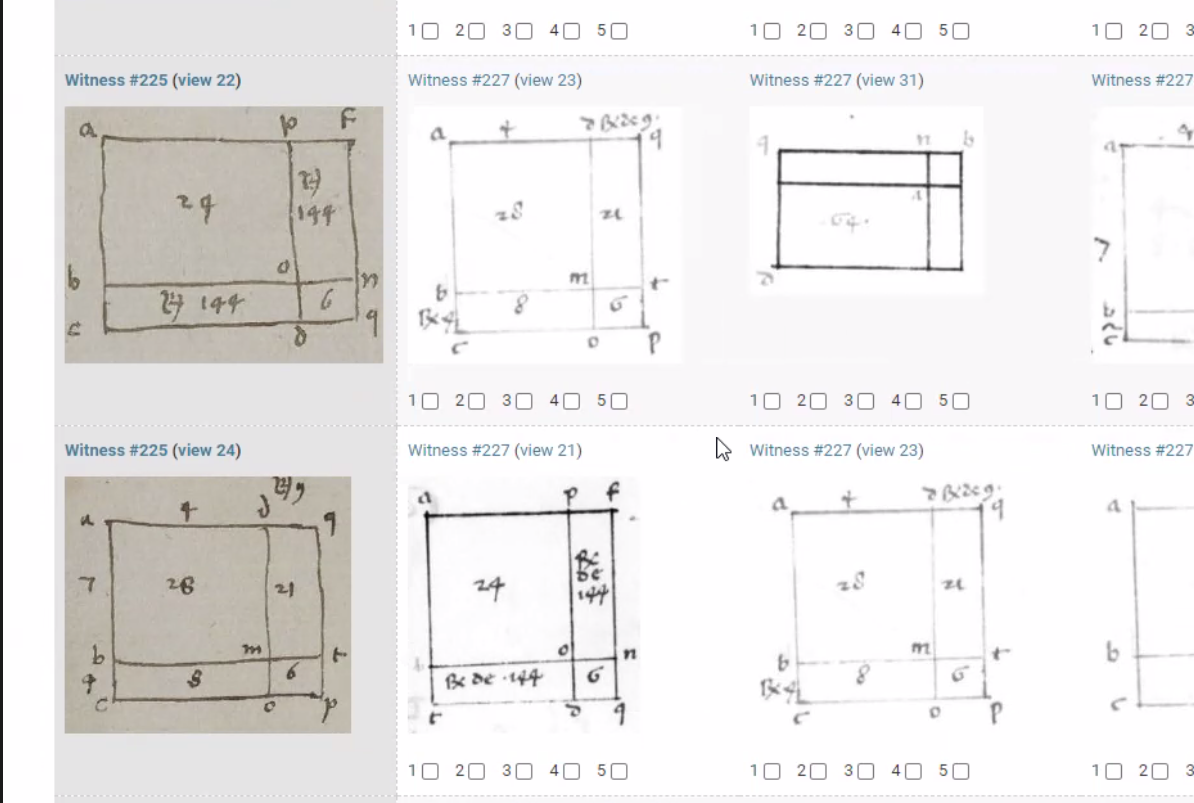
\includegraphics[height=7cm]{figues/label_dissim_exemple.png}
          \end{center}
          \caption{Impact des labels sur la recherche de similarité.}
          \label{fig:simlabel} \end{figure}

Devant ces difficultés il a été décidé d'adopter une annotation binaire
et basée uniquement sur le contenu graphique, partant du principe que
l'assignation d'un score de similarité par le modèle ne vaut pas pour
conclusion historiographique. Il sera toujours plus facile de ne pas
prendre en compte un résultat, et la visée de cet entraînement est
d'aboutir à un modèle assez extensif et généraliste. Il subsiste
cependant des dissensions au sein de l'équipe entre une définition très
stricte de la similarité, quitte à accepter des faux négatifs, et une
définition plus souple (typiquement, sensible aux labels), quitte à
créer des faux positifs. Pour concilier les besoins de tous les
chercheur.ses, il sera recommandé d'annoter selon la définition la plus
rigoureuse d'un point de vue scientifique, cette définition servant de
métadonnée aux chercheur.ses. Les annotations les plus souples seront
utilisées pour l'entraînement du modèle. Cette approche permet de
garantir une précision dans la classification des données tout en
offrant la souplesse nécessaire pour optimiser les performances des
algorithmes d'apprentissage automatique.

Ce cas d'étude est assez caractéristique des enjeux tenant à la
coordination au sein et entre des équipes de recherche dans le cadre du
développement d'un outil commun. D'où le développement des outils
d'annotation dans la plateforme commune assez généralistes pour que leur
usage s'adapte à des besoins différents et complexes\footnote{En
  réalité, les équipes de \vhs sont aussi passées à un classement binaire
  pour prévenir des problèmes de coordination au sein de leurs équipes,
  gardant l'usage des trois autres catégories pour une prochaine étape
  de fine-tuning.}.

\hypertarget{corpus}{%
\subsection{Corpus}\label{corpus}}

Les sources primaires d'\eida couvrent un spectre géographique et
temporel important. Orienté par les objectifs scientifique d'\eida --
arriver à une représentation globale des continuités et divergences qui
se tracent au cœur des pratiques astronomiques à travers l'histoire,
esquisser le voyage des sources à travers le temps et l'espace -- le
refus d'une vision eurocentrée justifie et explique une représentativité
large, servie par la constitution de cinq grands corpus issus de sphères
géographiques et temporelles diverses. Les manuscrits arabo-persans
produits entre le \textsc{viii}\ieme et le \textsc{xiii}\ieme siècle, des manuscrits latins
médiévaux produits majoritairement entre le \textsc{xiii}\ieme et le \textsc{xvi}\ieme siècle, les
manuscrits byzantins, produits entre les \textsc{ix}\ieme et \textsc{xv}\ieme siècles, les
manuscrits sanskrits, à partir du \textsc{xi}\ieme, et enfin les sources chinoises
datant du milieu du \textsc{xvi}\ieme siècle, après l'arrivée des premiers jésuites.
Le support de ces dernières n'est pas nécessairement le manuscrit, elles
prennent souvent la forme d'imprimés par blocs xylographiques dont les
matrices sont réemployées dans plusieurs témoins. Elles présentent donc
une forme hybride, sorte de pré-imprimé, qui posa des questions
complexes pour la modélisation conceptuelle des données.

Plusieurs centaines de manuscrits sont numérisés pour chaque tradition.
Sur ces numérisations, mises à disposition par les institutions
patrimoniales qui conservent ces témoins, seront appliquées les
traitements en prévision de l'analyse par les chercheur.ses, leur
permettant de souligner les motifs qui sous-tendent la diffusion
afro-eurasiens du modèle ptoléméen.

La gémellité avec \vhs impose un effort de modularité pour pouvoir
partager le modèle de données. Le travail de recherche de \vhs est mené
sur quatre corpus relevant, à l'instar de celui d'\eida d'une grande
diversité chronologique et géographique. Ces corpus se distinguent
cependant par une grande diversité thématique~: ils se composent de
manuscrits et d'imprimés concernant les sciences des mathématiques et
les sciences naturelles. Le premier corpus est le \emph{Physiologus},
rédigé vers le \textsc{ii}\ieme siècle à Alexandrie. Ce texte, l'un des plus
populaires du \ma, a contribué à l'émergence de la zoologie
chrétienne médiévale. Il a pour témoins 100 manuscrits grecs, dont treize
sont illustrés et réalisés entre le \textsc{xi}\ieme et le \textsc{xvi}\ieme siècle, contenant
environ 680 images d'animaux, de plantes et de minéraux. Le deuxième
corpus est le \emph{De materia medica} de Dioscoride, composé vers l'an
77 de notre ère. Ce traité pharmacologique destiné aux praticiens a été
largement diffusé et copié. Il est conservé dans 65 manuscrits grecs,
dont 17, réalisés entre le \textsc{vi}\ieme et le \textsc{xvi}\ieme{} siècle, sont illustrés et
contiennent environ 8340 images de plantes, d'animaux et de minéraux.
Les troisième et quatrième corpus se composent des planches de
l'Encyclopédie de Diderot et d'Alembert (1751-1772), les témoins de ce
travail couvrant une longue série de traités, dictionnaires et
encyclopédies au fil desquels les illustrations ont été copiées et
retravaillées. Leur étude se focalise aussi sur leur inclusion
ultérieure dans des encyclopédies telles que l'Encyclopédie méthodique.
Le troisième corpus se concentre sur l'Histoire naturelle (Zoologie),
tandis que le quatrième porte sur les sciences mathématiques\footcite{noauthor_vhs_nodate}.

Le deux corpus jumeaux diffèrent aussi en taille~: celui de \vhs présente plus de 2000 témoins devant 300 pour \eida.

Malgré ces divergences importantes, les données sont issus de spectres
assez larges pour opérer des croisements dont l'exploitation peut
s'avérer fructueuse~: les corpus \vhs présentent quelques diagrammes
astronomiques, et les manuscrits \eida présentent plusieurs images de
plantes. La mise en commun des résultats permet d'établir des liens
entre le \ma (focus d'\eida) et la période moderne (focus de \vhs)
pour les domaines respectifs étudiés. Notamment, des chercheur.ses d'\eida
s'intéressent à la transition du manuscrit à l'imprimé. La possible
jonction des corpus reste néanmoins problématique, et les modèles d'\ia doivent être spécialisés sur les objets d'étude respectifs des deux projets.

Ces remarques sont révélatrices de l'entre-deux qui nous intéresse dans
ce mémoire~: bien que les projets aient un objectif et des objets
d'étude précis, ceux-ci se trouvent élargis par le réseau institutionnel
et les dynamiques collaboratives qui accompagnent la création des outils
numériques. Le niveau de modularité de l'outil créé devra prendre en
compte cette généralisation possible sans perdre de vue les objectifs
initiaux des deux projets.

\hypertarget{modele-de-donnees}{%
\subsection{Modèle de données}\label{modele-de-donnees}}

L'application commune à \vhs/\eida est développée avec le \textit{framework} Django
et adossée sur une base de données gérée avec PostgreSQL. Le modèle de
données conçu pour l'application a fait l'objet de réflexions et
réadaptations pour répondre aux besoins de description des sources de
\vhs et \eida, tout en restant suffisamment flexible pour être utilisé par
d'autres projets souhaitant reproduire les méthodes employées par les
deux projets. Le défi consiste à conceptualiser la donnée de manière
suffisamment spécifique et assez généraliste.

\hypertarget{modele-initial}{%
\subsubsection{Modèle initial}\label{modele-initial}}

Le modèle de données initialement construit\footnote{Voir l'annexe \ref{data_models} pour une illustration de l'évolution du modèle de données.} pour
l'application \vhs prévoit l'existence des entités 'manuscrit' et
'imprimé', qui correspondent aux supports représentés dans
les corpus d'\eida et de \vhs. Ces deux \emph{états matériels} du texte
sont reliés à une entité plus abstraite~: le \wo.
S'appuyant sur la définition de \wo que donne le CIDOC-CRM\footnote{Le
  modèle conceptuel définit, dans un domaine donné, comment représenter
  la réalité. À ce titre il est indépendant de la manière dont on stocke
  les données informatiquement. Né dans le domaine des musées, CIDOC-CRM
  est un modèle conceptuel standardisé pour la modélisation des
  informations dans le domaine du patrimoine. Il vise à décrire et à
  rendre interopérables des objets du monde culturel en général. La
  notion d'événement se trouve au cœur du modèle, traduisant une
  approche monotonique des données~: les objets décrits peuvent évoluer,
  on peut toujours décrire de nouveaux événements liés à cet objet.
  Ainsi, on n'aura potentiellement jamais terminé de décrire un objet en
  CIDOC-CRM.}, un \wo est indépendant de sa forme matérielle, c'est une
production intellectuelle qui peut se manifester dans différentes
sources, pouvant elles-mêmes présenter des variations.

Mais ce premier modèle va rapidement montrer des limites, notamment
liées à la description d'une même œuvre divisée en plusieurs ouvrages,
ou d'un ouvrage contenant plusieurs œuvres. De plus, la pertinence de la
distinction absolue des manuscrits et imprimés ne permet pas une
description pertinente de tous les objets~: par exemple les sources
chinoises, dont le support n'est pas nécessairement le manuscrit,
prennent souvent la forme d'imprimés par blocs xylographiques dont les
matrices sont réemployée. Ces constats ont mené à la refonte de ce
modèle de données. 

\hypertarget{premiere-refonte}{%
\subsubsection{Première refonte}\label{premiere-refonte}}

Le nouveau modèle est non seulement plus pertinent mais aussi déjà plus
flexible. Il est centré autour de l'entité 'témoin' ou \wit, et
est complété par d'autre tables pour décrire la diversité des sources et
leurs différents modes d'existence. Ainsi, les séries héritent
uniquement des imprimés et les témoins héritent à la fois des
manuscrits et des imprimés. Une \ser est une édition en
plusieurs volumes d'une œuvre imprimée. Le témoin ramène à chaque volume
en tant qu'entité matérielle de référence, ou à un manuscrit. Il peut
contenir un ou plusieurs 'travaux' (\wo)~; un même \wo peut
correspondre à des séries et des témoins différents (table de relation
\textit{Content}). La table \wo inclut donc les références au lieu et à l'auteur
(clés étrangères), mais aussi l'information relative à la plage de temps
durant laquelle cette œuvre a existé physiquement (durant laquelle on
atteste l'existence de témoins). La ou les numérisations
(\digits) sont reliées au \wit et contiennent les détails sur la
source de numérisation et l'état des traitements via \iiif\footnote{Voir le \hyperlink{iiif}{Chapitre 2} sur \iiif}. Une entité Tag est utilisée comme moyen de
différencier manuscrit, imprimé ou gravure, et la table de relation
\textit{Tag\_Exemplar} fait le lien entre le témoin et les tags. La table
\textit{Role} établit des relations entre des contenus (\textit{Content}), des
\emph{séries} (\sers) et des personnes (\textit{Persons}), attribuant à
ces dernières les rôles d'auteur ou d'éditeur.

Les évolutions en cours pendant mon stage, détaillées en partie
III\footnote{Voir le \hyperlink{chapitre-7-processus-et-fonctionnalites}{Chapitre 7}}, ont nécessité de faire des choix
complexes, répondant à une double exigence \emph{a priori} paradoxale~:
une plus grande flexibilité pour intégrer de nouvelles sources de
données et une précision de description suffisante. De nouvelles
questions ont été soulevées liées à la granularité et à la cohérence
sémantique.

Ce paradoxe apparent met en lumière les défis et la complexité liés à la
modélisation de la donnée, et les transformations successives reflètent
des questionnements~: comment rendre l'application la plus universelle
possible, l'ouvrir à une large diversité de sources, sans renoncer à la
qualité de la description des sources des projets de \eida et \vhs~?
Comment, d'ailleurs, conceptualiser un modèle qui convienne aux deux
projets et leurs objectifs~? Les solutions ci-dessus décrites sont
satisfaisantes mais amenées à évoluer, montrant que la modularité se
construit sur le temps long.
                    
                \hypertarget{normalisation-donnees}{\section{%
                La normalisation des données d'annotation}\label{normalisation-donnees}}
                    \gaga mène une réflexion
méthodologique sur la portabilité des modèles, leur diffusion et le
partage de grands ensembles de données annotées selon des normes
communes. Les modèles d'\ia, notamment ceux dédiés à la
reconnaissance du texte manuscrit (\htr) et au traitement automatique des
langues (\tal), requièrent des données d'entraînement spécifiques. 

Mais si chaque projet de recherche annotait ses corpus selon ses propres
exigences, ils engendreraient fatalement des silos de données non
réutilisables. Pour garantir la réutilisation des données, il est
impératif d'établir des normes et des standards.

Le projet porte alors le développement d'une syntaxe
d'annotation générique pour harmoniser la segmentation des pages des
vérités de terrain, afin de constituer des corpus d'entraînement réutilisables. \gaga propose une
approche très inclusive en identifiant des éléments textuels communs à
une large variété de documents, manuscrits comme imprimés. Cette
démarche donne lieu à la définition d'un vocabulaire contrôlé permettant
ainsi de construire des corpus annotés compatibles avec différents contextes\footcite[``Using a common vocabulary to annotate zones called SegmOnto (that is still evolving), we have developed a generic workflow to analyse the layout, OCRise the text, and convert the ALTO output into minimally encoded TEI files (\dots).''][p.2]{janes_towards_2021}~:
SegmOnto\footnote{https://github.com/SegmOnto}

Les étapes de lemmatisation et d'étiquetage morphologique (POS-tagging) effectuées par les modèles de \tal sur le texte extrait des pages numérisées visent à normaliser le
langage en réduisant les mots à leur forme canonique (lemme) et en
identifiant leur catégorie grammaticale. Cette normalisation est
essentielle pour faciliter des analyses ultérieures telles que la
collation et la stylométrie. Elle permet une analyse comparative des textes
malgré la grande variabilité inhérentes aux
langues historiques, pour lesquelles l'absence de normes orthographiques entraîne une
grande diversité de graphies. La préparation des données, là aussi, a donné lieu à une
réflexion méthodologique sur les défis liés à la standardisation des
annotations linguistiques dans les corpus diachroniques.

Selon \citeauthor{gabay_standardizing_2020}~:
\begin{kwote}                     
	``With the development of big corpora of various periods, it becomes
	crucial to standardise linguistic annotation (e.g.~lemmas, POS tags,
	morphological annotation) to increase the interoperability of the data
	produced, despite diachronic variations.''\footcite[p.2]{gabay_standardizing_2020}
\end{kwote}  

\citeauthor{gabay_standardizing_2020}\footcite{gabay_standardizing_2020} relèvent la
difficulté de mettre en œuvre un cadre technique qui prenne en compte
les pratiques d'annotation déjà établies et propres à des états de la langue. Pourtant garantir une
interopérabilité minimale avec les corpus existants est essentielle pour
maximiser la valeur ajoutée des nouvelles données.

\begin{kwote}                     
	``Such a task cannot be done without taking into account longstanding
	annotation practices, in order to allow (minimal) interoperability with
	already existing datasets. Such a statement is sadly easier said than
	done, because EMF is an intermediary stage between medieval (12th-15th
	c.) and late modern and contemporary (from c.~1750) French, two states
	of language that tend to have different needs regarding annotation: EMF
	is then caught in between two (potentially incompatible) practices, one
	for each extreme of the continuum.''\footcite[p.2]{gabay_standardizing_2020}
\end{kwote}     

Il est particulièrement complexe de trouver un équilibre entre une
description linguistique trop fine, qui pourrait limiter
la réutilisabilité des corpus, et une description trop générale, qui pourrait
manquer de précision. De plus, les besoins en annotation varient considérablement
entre le français médiéval et le français moderne, et les systèmes
d'annotation de ses deux états de la langue sont difficilement
réconciliables~: or une large partie des sources de \gaga se
situent dans l'entre-deux. Trouver un compromis qui satisfait les
exigences spécifiques de chaque période est complexe.

L'harmonisation des annotations vise à favoriser la diffusion des corpus
de données sur HTR-United, une plateforme collaborative dédiée au
catalogage de vérités de terrain pour l'\htr et l'\ocr, principalement en
français\footcite{chague_htr-united_2021}. Cette base de
données, hébergée sur GitHub, centralise des images et leurs
transcriptions produites par différents projets de recherche, offrant
ainsi une diversité de jeux de données diachroniques et géographiques
pour l'entraînement de modèles \htr.

\gaga vise aussi à la diffusion des modèles en eux-même, qui peuvent alors être réutilisés et spécialisés. Par ailleurs, le projet
s'appuie sur des outils existants, par exemple Deucalion, une boîte à
outils de traitement automatique des langues (\tal) conçue pour être
interopérable avec d'autres systèmes\footnote{https://github.com/chartes/deucalion-model-af}.
                    

              


\vspace{2cm}


Les apports et les réflexions du projet \gaga reflètent la problématique globale de ce
mémoire~: comment concevoir des cadres pour l'environnement de la
recherche en Humanités Numériques, tout en répondant aux exigences
scientifiques de chaque projet. On voit se filer avec ce cas d'étude un écosystème complexe dans lequel s'agencent des systèmes et protocoles généraux et extensibles, adaptables aux besoins locaux, comme la \tei, ou SegmOnto, ou encore des \api pour la récupération des données. De nombreux défis restent cependant à relever, montrant que l'interopérabilité universelle est un idéal difficilement atteignable.

L'utilisation de l'\ia porte la question du partage des ressources à un niveau d'importance supérieur, puisque les modèles peuvent être spécialisés, et les corpus enrichis produits peuvent constituer des données d'entraînement. L'intervention du chercheur.se pour corriger les résultats des traitements automatiques est donc un aspect important à prendre en compte pour assurer la fiabilité scientifique de ses corpus annotés. 

\gaga visait à l'élaboration d'un
outil d'acquisition et d'enrichissement des données capable de se
détacher d'un corpus spécifique et sur ce point se voulait preuve de concept, mais le projet
n'a pas pleinement atteint ses objectifs, car la chaîne de traitement est restée très orientée vers les corpus de la \bnf. Il a ainsi mis en
évidence la complexité de concilier les exigences d'une infrastructure
générique et les besoins spécifiques des données, montrant que la modularité s'inscrit avant tout dans le temps. 

Comme le montre le cas de e-Scriptorium, une chaîne de traitement, si elle est assez généraliste pour tolérer une grande diversité de données, participe à la cohérence des pratiques et à la mutualisation des outils de la recherche. Les modalités d'accès (notebooks, plateforme, scripts etc.) impactent la prise en main et l'adoption des outils. 

Plus généralement, les recherches menées sur l'enrichissement et l'exploration de larges corpus grâce aux outils d'\ia ouvrent de nouvelles perspectives en terme de trouvabilité et de fouille de données visuelles ou textuelles. Cette valeur ajoutée est liée au passage du format \jpeg à des formats balisés et sémantiquement riche qui permettent des exploitations ou l'indexation. 
            
        \clearemptydoublepage
        
\chapter*{Conclusion partielle}
Comme le dit \citeauthor{jacquot_decrire_2017}\footcite{jacquot_decrire_2017}, face aux problématiques de traitement du volume, ``une réponse peut résider dans la généralisation des outils et
des méthodes ainsi que dans le partage des récits de projets de
recherche antérieurs, forme d'apprentissage et d'échange importante.''

Un trait saillant dans la progression vers l'automatisation est la
confrontation de deux besoins~: la collaboration et la spécialisation. D'un côté, la communauté scientifique voudrait mutualiser les outils et les méthodes, afin d'encourager le partage d'une expertise interdisciplinaire, des moyens financiers, et d'améliorer la maintenabilité, contribuant
ainsi à la robustesse des développements. Un tel outil, à l'image de la plateforme e-Scriptorium, qui porte et guide les processus de transcription de texte, et dont la portabilité facilite l'intégration dans divers écosystèmes de recherche, contribue aussi à la cohérence des méthodes scientifiques au sein d'une équipe de recherche, ou entre plusieurs projets. De l'autre côté, il faut prendre
en compte les spécificités locales des données, les besoins des
utilisateur.rices et les enjeux propres aux projets de recherche qui portent
la création des outils de traitement. Les solutions doivent être
adaptées aux particularités des corpus et aux questions de recherche
spécifiques, ce qui peut parfois entrer en conflit avec la nécessité de
généralisation. 

On aura voulu montrer dans cette première partie que l'ambition de créer un
outil générique -- visant à l'enrichissement et la sémantification de la
donnée -- se heurte à des dynamiques collectives et à la multiplicité des
acteurs, autant qu'elle en profite. La philosophie de l'ouverture, à la
fois des données et du code, est un atout (libre accès aux sources,
appui sur des scripts et des projets de recherche existants, rencontres
avec d'autres projets, création des synergies avec d'autres équipes ou
institutions et mutualisation des moyens financiers et humains), et une
double contrainte. La première est la nécessité d'assurer une
interopérabilité technique pour ouvrir en retour les corpus et garantir
la reproductibilité des résultats. La deuxième porte sur la prise en
compte de l'hétérogénéité des données, ce qui demande de trouver le
juste équilibre entre précision et flexibilité en terme de
description.

Nous sommes restés volontairement vagues sur la question des modèles de
vision artificielle et les réseaux de neurones~: ils sont pourtant la
clé de voûte des processus d'enrichissement et d'exploration des données. La construction et l'entraînement des réseaux de neurones s'inscrit aussi dans une balance
délicate entre généralisation et spécialisation. Les modèles doivent
être suffisamment généralistes pour reconnaître et interpréter une large
variété de motifs provenant de contextes divers, ce qui leur permet
d'être applicables à la diversité des scénarios rencontrés et de gérer
l'hétérogénéité des grands corpus~: par exemple la grande variété
orthographique, morphologique et de mise en page dans le cadre du projet
\gaga. Mais l'efficacité des modèles de vision exige aussi leur
spécialisation sur des jeux de données étroitement ciblés. Par
conséquent, les chercheur.ses et ingénieur.es doivent constamment équilibrer
ces deux exigences pour développer des modèles robustes, polyvalents,
mais aussi suffisamment précis pour répondre aux besoins spécifiques des
applications en recherche.

    \part{Mise en œuvre et exploitation de la \emph{Computer Vision}}

\chapter*{Introduction partielle}

Les diagrammes astronomiques offrent une perspective unique sur la
compréhension et la diffusion du savoir à travers les
siècles dans l'histoire afro-eurasienne. Des centaines de manuscrits
numérisés et des milliers de diagrammes sont disponibles. Nous avons
constaté dans la première partie de ce travail les dimensions et
l'hétérogénéité importantes caractérisant ce corpus de recherche, ainsi
que l'impossibilité de réaliser des annotations à grande échelle pour
chaque tâche spécifique. Pour assister les chercheur.ses dans le travail de
fouille et d'analyse des documents historiques, diverses méthodes
d'apprentissage profond (\dl) ont été développées et
implémentées sur la plateforme.

Il ne s'agit pas seulement d'implémenter des outils d'\ia efficaces,
mais aussi d'en exploiter les résultats. Pour \eida, la finalité est de
pouvoir produire des éditions scientifiquement satisfaisantes des
diagrammes.

Qu'est-ce que la vision artificielle~? Comment rendre les modèles
efficaces sur les sources historiques~? Notre propos s'articulera autour
de trois axes principaux~: le fonctionnement des modèles de vision, les
enjeux tenant aux jeux de données pour leur entraînement, et la
conceptualisation de l'outil d'édition qui repose sur les résultats des
algorithmes.

\clearemptydoublepage
    
        \hypertarget{chapitre-4-modele}{%
        \chapter{Les modèles de \emph{Computer Vision}}\label{chapitre-4-modele}}

            Dans des termes très simples, pour faire exécuter une tâche à la
machine, deux solutions existent. La première consiste à écrire un
programme, dont l'expert métier a explicité les règles. Le programme est
entièrement rédigé par un.e développeur.se. Il effectue une tâche précise,
chaque conjecture spécifique doit être prévue et son traitement
clairement formulé. Si le code produit des erreurs, il doit être modifié
par le.a développeur.se. La deuxième approche consiste à donner au programme
la capacité de se modifier lui-même, sans que cette modification soit
explicitement rédigée. L'expert métier doit coder l'architecture du modèle et
annoter des exemples ; puis un seul algorithme (d'apprentissage) suffit pour
traiter de multiples cas réels. En cas d'erreur de l'algorithme, il faut agir non plus
sur le programme mais sur les exemples d'apprentissage. L'objectif est
d'apprendre à généraliser pour prédire sur des exemples non vus pendant
l'apprentissage\footcite[p.7]{chollet_apprentissage_2020}.

\begin{kwote}         
``On peut ainsi opposer un programme \emph{classique}, qui utilise une
procédure et les données qu'il reçoit en entrée pour produire en sortie
des réponses, à un programme \emph{d'apprentissage automatique}, qui
utilise les données et les réponses afin de produire la procédure qui
permet d'obtenir les secondes à partir des premières.''\footcite[p.1-2]{azencott_introduction_2022}
\end{kwote} 

L'émergence de l'apprentissage machine a alors ouvert de nouvelles
perspectives en permettant de modéliser des interactions complexes entre
les données. Les modèles de \dl sont également plus
résilients face aux variations et au bruit présents dans les
données\footcite{juneja_deep_2023}. Ainsi,
l'application de l'apprentissage profond se révèle particulièrement
pertinente dans le cadre d'\eida, car elle permet de relever le défi
de la sémantification des images, y compris lorsqu'il s'agit de sources
historiques complexes.

        \hypertarget{les-reseaux-de-neurone}{%
        \section{Les réseaux de neurones, ou la généralisation prise au sens
        mathématique}\label{les-reseaux-de-neurone}}
         
L'astronomie est issue d'une tradition continue vieille de près de 4000
ans qui transcende les cultures et les langues. Les théories, les
savoirs, les méthodes, au gré de leur diffusion, se mélangent aux
pratiques autochtones pour servir les usages locaux, qui bien souvent
renforcent des dynamiques de pouvoir en place, que ce dernier soit
politique ou religieux. Les sciences astrales revêtent ainsi une
importance culturelle majeure.

Une étude approfondie des sources révèle les processus par lesquels les
connaissances se sont enrichies et transformées au contact de
différentes cultures. Leur examen permet en outre de souligner les
spécificités et les innovations de chaque tradition, tout en montrant
les interconnexions et les influences réciproques qui ont façonné
l'évolution de l'astronomie. Les schémas de circulation sont dans de
nombreux cas de très grande portée géographique, chronologique et
culturelle. Ils relient des contextes de production de connaissances à
l'échelle afro-eurasienne et sur des périodes de siècles voire de
millénaires. La trace de ces transmission supporte une vision connectée
et globale de l'histoire des cultures et du savoir.

La grande diversité des sources et des approches possibles rend
cependant difficile une approche globale. À ce titre, il est important
de cibler un objet d'étude : \eida se focalise ainsi essentiellement dans
la transmission de la tradition ptoléméenne, et le corpus se compose
donc de ressources manuscrites et imprimées relevant de cette tradition.

\hypertarget{ptolemee-modele-et-transmission}{%
\subsection{Ptolémée : modèle et
transmission}\label{ptolemee-modele-et-transmission}}

Ptolémée tient une place proéminente dans l'histoire de l'astronomie et
des mathématiques. Son nom reste associé à la conception d'un système
astronomique qui plaçait la Terre immobile au centre du monde, et dont
la mise en question, de Copernic à Newton, a commandé la révolution
scientifique.

Dans sa \emph{Syntaxe mathématique}, plus connue sous le titre
d'\emph{Almageste}, et dont la dernière observation consignée date de
141, il expose l'ensemble des connaissances astronomiques de son époque.
Notamment il perfectionne le modèle élaboré par Hipparque, à qui il
emprunte la découverte de l'excentricité des trajectoires apparentes du
Soleil et de la Lune par rapport à la Terre, et l'idée de composer ces
trajectoires à l'aide de deux mouvements distincts. Il élabore un
système géocentrique au moyen d'un ensemble complexe de trajectoires
circulaires des objets pris dans un mouvement uniforme : les déférents,
autour de la Terre, et les épicycles, dont les centres parcourent les
déférents\footcite{lequeux_systeme_nodate}.

En effet, les sociétés anciennes attendent des
corps astraux (soleil, lune, planètes et étoiles) un mouvement uniforme
et le plus ``parfait'' possible, c'est-à-dire un cercle. Pourtant la
trajectoire de ces corps, observée empiriquement, n'est pas circulaire.
Le modèle de Ptolémée explique ces imperfections en postulant que les
mouvement apparemment irréguliers sont dû à cette fameuse combinaison de
plusieurs trajectoires circulaires régulières vues depuis la Terre,
point statique. Les planètes se déplacent à vitesse uniforme sur un
cercle (l'épicycle) dont le centre se déplace à vitesse uniforme sur un
cercle coplanaire (le déférent), dont la Terre est le centre.

En plus de la description du mouvement des astres, Ptolémée dresse dans
l'\emph{Almageste} des tables établissant les positions de la lune et
prévoyant les périodes et les caractéristiques des éclipses avec une
précision inédite\footcite{raymond_jones_ptolemy_2024}, un catalogue des étoiles, un traité
complet de trigonométrie plane et sphérique et une description des
instruments nécessaires à un grand observatoire.

L'œuvre de Ptolémée fera référence, et en tant que synthèse des
connaissances astronomiques antérieures, sa transmission correspond
à celle de la vision des pratiques de l'astronomie grecque à son apogée,
et sa diffusion façonnera la production astronomique ancienne pendant
près de treize siècles. D'ailleurs le nom d'Almageste date de la
transmission par les civilisations arabes à l'occident.

En effet, lors de la chute de l'Empire Romain d'occident, la majeure
partie des ouvrages antiques sont perdus et la science occidentale
stagnera jusqu'au \textsc{xii}\ieme siècle. Elle continuera cependant à progresser
ailleurs : notamment dans le monde arabe et musulman. Dès le \textsc{viii}\ieme et
\textsc{ix}\ieme siècle, les Arabes vont traduire dans leur langue la plupart des
grands textes scientifiques de l'Antiquité, en particulier les œuvres
d'Aristote et l'\emph{Almageste} de Ptolémée. Sans remettre en cause le
géocentrisme et le système de Ptolémée, ils le perfectionnent et
l'amènent à un très grand degré de précision. Nécessaire à la stricte
observation des règles de l'islam, l'astronomie arabe se développe et se
diffuse, grâce aux travaux d'al-Biruni, al-Hazen ou al-Sufi\footcite{noauthor_monde_nodate}.

À partir du \textsc{xi}\ieme et surtout du \textsc{xii}\ieme siècle, au fil des conquêtes des
occidentaux en Espagne et en Sicile, les textes grecques sont traduits
en latin via la traduction arabe. La transmission des savoirs
gréco-arabes -- notamment les traductions arabo-latines de
l'\emph{Almageste} et du Livre des étoiles fixes d'al-Sufi -- ouvre la
voie à un renouveau scientifique dans l'Occident chrétien, permettant
ainsi l'essor des grandes universités européennes de l'époque (Paris,
Oxford, Bologne, etc). On redécouvre les modèles d'Aristote et de
Ptolémée en les adaptant aux conceptions chrétiennes\footcite[``Le
  système géocentrique devient le modèle astronomique et théologique de
  l'Église, qui ne remet pas en cause la sphéricité de la Terre''][]{noauthor_monde_nodate}.

Avant l'avènement de l'astronomie grecque, les Babyloniens, dès le premier
millénaire \jc, utilisaient des calculs arithmétiques pour prévoir
la position des planètes. Ces théories ont voyagé jusqu'en Perse et en
Inde, où elles ont été adaptées et combinées à des méthodes autochtones.
Les théories grecques de l'époque de Ptolémée et de son prédécesseur
Hipparque sont également parvenues jusqu'en Inde, créant un matériel
complexe dont les influences sont difficiles à démêler. Parmi les
pratiques empruntées aux théories grecques, on relève l'emploi de termes
-- par exemple le titre du canon \emph{Romaka Siddhanta} datant du début
du \textsc{v}\ieme et qui marque les origines de la science astronomique sanskrite --
ainsi que des modèles épicycliques et des méthodes de calculs requérant
des paramètres numériques hérités d'Hipparque\footnote{\cite[p.6-7]{mercier_studies_2004} in \cite[p.15]{albouy_mediation_2019}}.

La tradition chinoise se développe de manière relativement indépendante
et les échanges ne débutent qu'autour de 200 \jc. Elle se distingue
de celle des Grecs par un intérêt plus marqué pour la prédiction
d'événements singuliers plutôt que pour les théories cosmologiques
cherchant l'établissement d'un modèle d'organisation du ciel. En effet,
en Chine impériale, l'astronomie a une fonction politique. L'empereur
est considéré comme le Fils du Ciel et ainsi la régulation du
calendrier, ou bien le succès (ou l'échec) de ses astronomes à prédire
une éclipse, se reflétaient positivement ou négativement sur lui.
L'inclusion croissante des diagrammes dans les traités après les
missions jésuites à partir du \textsc{xvi}\ieme siècle révèle l'influence des
pratiques d'Europe de l'ouest.

Pour conclure, l'\emph{Almageste} se présente donc comme une sorte
d'encyclopédie des connaissances d'une époque qui s'est enrichie avec le
temps au point de rendre difficile l'appréciation de son état originel.
Œuvre sans cesse recopiée au cours des siècles, passant du grec à
l'arabe puis au latin, transmise à travers tout le bassin méditerranéen
et dominant le \ma occidental après avoir conquis l'Islām, chaque
traduction et chaque copie de l'Almageste n'ont pas seulement transmis
son contenu, mais l'ont aussi adapté et enrichi en fonction des
contextes culturels et scientifiques de chaque époque. L'œuvre
ptoléméenne a servi de base à de nombreux commentaires et traités,
intégrant progressivement des éléments de connaissance issus de diverses
traditions scientifiques, et illustrant ainsi l'interconnexion des
savoirs à travers les civilisations.

\begin{kwote}
``Certains indices dans les manuscrits révèlent les emprunts
intellectuels qui s'opèrent au fur et à mesure des copies ; les méthodes
de calcul, le tracé des diagrammes, la mise en page des tables, la
structuration des textes techniques, la mention d'auteurs antérieurs, la
réutilisation de paramètres astronomiques ou même la récurrence de
certaines erreurs sont autant de signes qui témoignent des échanges
culturels qui ont façonné la pratique de l'astronomie.''\footcite[p.14]{albouy_mediation_2019}
\end{kwote}

Comme l'entend \citeauthor{albouy_mediation_2019}, les diagrammes font partie des révélateurs des
échanges intellectuels.

\hypertarget{le-diagramme-vecteur-de-connaissances}{%
\subsection{Le diagramme vecteur de
connaissances}\label{le-diagramme-vecteur-de-connaissances}}

L'historiographie et l'histoire des sciences n'échappent pas au récent
``visual digital turn''\footcite[``Digital humanities research has
  focused primarily on the analysis of texts. This emphasis stems from
  the availability of technology to study digitized text. Optical
  character recognition allows researchers to use keywords to search and
  analyze digitized texts. However, archives of digitized sources also
  contain large numbers of images.''][]{wevers_visual_2020} général des
humanités, montrant à quel point la production et la diffusion du savoir
croisent les représentations visuelles rendant compte de ces
connaissance. De fait, on ne s'intéresse plus seulement au texte. Or les
astronomes, au fil de l'histoire, ont eu recours à un grande diversité
de matériaux. Les sources primaires sont constituées par des instruments
et des écrits, ces derniers eux-même hétérogènes. Dans les traités
anciens, on trouve des descriptions détaillées, des propositions
mathématiques, des tables de calcul, et des diagrammes illustrant
souvent le texte qu'ils accompagnent. Les sources primaires peuvent en
outre être enrichies de commentaires et de gloses, prose ou
illustrations, témoignant de la manière dont les connaissances ont été
transmises et interprétées. Elles révèlent également les méthodes
pédagogiques employées pour enseigner ces savoirs.

Au cœur de cette diversité, le diagramme, objet hybride pour deux
raisons : il combine un contenu géométrique (des lignes, arcs et
cercles) et des labels, et il entretient un lien (plus ou moins étroit)
avec le texte qui l'accompagne.

En tant que structure de pensée, la figuration géométrique -- une forme
de création de modèles associée à l'élaboration et à la résolution de
problèmes dans divers domaines de la pensée humaine liés au calcul
abstrait et à la modélisation des idées -- est aussi ancienne que
presque toute autre forme d'enregistrement des pensées et des idées. Des
diagrammes utilisés pour calculer la superficie de parcelles et de
terres apparaissent dans le Papyrus mathématique Rhind, la source la
plus importante qui subsiste pour l'histoire des mathématiques dans
l'Égypte ancienne\footcite[p.6]{safran_diagram_2022}. Instruments
de pensée et de démonstration, ils servent non seulement à transmettre
le savoir mais aussi à le produire. Et dans un étrange mouvement
métaréflexif, ils permettent aux historien.nes des sciences de produire la
connaissance sur ces anciennes traditions heuristiques et leur
transmission.

Les diagrammes sont, pour les astronomes, le support d'une pratique
scientifique, et sont ainsi révélateurs de leurs méthodes, de leur
contexte d'exercice et de leur conception de leur discipline. Ils
revêtent des rôles et des aspects différents, permettant d'identifier
des modes diagrammatiques\footnote{La ``diagrammatisation'' désigne
  assez largement l'investissement des acteurs dans la complexification
  des représentations visuelles des propositions scientifiques présentes
  dans les traités.} spécifiques d'un lieu ou d'une époque, et traçant
des lignes de diffusion des pratiques et des savoirs.

Au \ma, trois grandes cultures coexistent en Eurasie : les
cultures byzantine, islamique, et d'Europe occidentale. Elles
connaissent des évolutions différentes en termes linguistiques et
religieux ; cette diversité est vraie également pour les usages auxquels
les diagrammes astronomiques étaient destinés, pour les domaines dans
lesquels ils étaient reconnus comme des instruments de pédagogie et des
vecteurs de pensée, ainsi que pour la place accordée à la culture
visuelle plus généralement et aux modes de représentation
diagrammatiques. Pourtant cette coexistence donne lieu à des échanges
intellectuels, artistiques, diplomatiques et commerciaux. Les
traductions d'œuvres savantes, les transferts de manuscrits illustrent
la porosité des frontières du savoir et de l'interdépendance des
cultures. Les diagrammes astronomiques sont à ce titre témoins des
chemins de diffusion des connaissance et des pratiques des sciences.

\emph{Comment ces diagrammes parlent-ils aux historien.nes ?}

Les diagrammes peuvent être étudiés intrinsèquement (quelles conventions
gouvernaient le langage visuel, quelle fonction assumaient-ils ?) ou
extrinsèquement (pour comprendre la transmission de ces traditions et
ces pratiques entre l'Europe et l'Asie, en passant pas la péninsule
arabique).

On pourrait penser que les formes et éléments visuels
utilisés pour une démonstration géométrique soient universels, qu'ils
restent les mêmes quelle que soit la date et la langue de l'explication
textuelle, le grec, l'arabe ou le latin\ldots{} Et pourtant le contexte
géographique, temporel, et les aspects matériels liés aux technologies
d'inscription changent profondément le fonctionnement et les objectifs des diagrammes,
leurs objectifs.

L'évolution des conventions graphiques en sont un exemple frappant. Par
exemple, l'axe vertical de la Terre, bien que représenté à plat sur la
page, fut conventionnellement compris comme un axe perpendiculaire à la
coupe du globe. Au fil du temps, de nouvelles conventions graphiques ont
été adoptées, et pour les lecteurs d'aujourd'hui on représenterait
sûrement le globe terrestre avec sa profondeur pour expliciter la
représentation. Citons en outre la représentation des phases lunaires,
qui a connu une évolution concernant l'association des couleurs claire
et sombre à la pleine lune et à la nouvelle lune. Si aujourd'hui on
associerait plutôt la pleine lune à un aplat de couleur claire et la
nouvelle lune à une couleur sombre, les manuscrits médiévaux byzantins
adoptent le référentiel contraire.

De même, le rôle du diagrammes est fluctuant, et va au delà du simple
support démonstratif au service du texte. Par exemple ceux des
\emph{Traités logiques} d'Aristote ont probablement circulé
indépendamment du texte, même si tout indique que les écrits les
appelaient dès le départ. Cela souligne la distinction entre le
diagramme en tant qu'objet de démonstration et de discussion complétant
une proposition d'un côté, et le diagramme en tant qu'accompagnement des
textes scolaires, qui aide à la compréhension de l'autre\footcite[p.5]{safran_diagram_2022}. Le
diagramme peut ainsi constituer la preuve et le support d'une
réinterprétation de la proposition textuelle.

Par-dessus tout, les transformations subies au fil des copies et des
réceptions sont éloquentes pour les chercheurs. Bien que les diagrammes
soient initialement conçus pour clarifier et expliquer une proposition textuelle, ils peuvent
parfois être des vecteurs de confusion (ou d'innovation). Le même diagramme d'une même
œuvre soumis à un processus constant de transformation par les scribes,
les artistes ou les lecteurs/commentateurs. 

La recherche des erreurs
transmises a ainsi un intérêt philologique important. Les cas de
méprises et les malentendus sont peut-être plus nombreux que les cas de
compréhension fidèle lors de la traversée des frontières géographiques,
culturelles, religieuses et/ou linguistiques, et l'étude des erreurs et modifications
révèle leurs aspects heuristiques, autant qu'il peut amener à
l'établissement d'un stemma\footcite{raynaud_building_2014}.

L'importance des diagrammes dans les transmissions est illustrée par l'exemple des diagrammes attribués à al-Ḥajjāj, en lien avec la transmission arabe des \emph{Éléments} d'Euclide. Bien que la traduction originale d'al-Ḥajjāj soit perdue, les diagrammes retrouvés dans divers manuscrits montrent qu'il utilisait parfois des schémas différents de ceux adoptés dans la tradition arabe ultérieure. Ces diagrammes ont probablement joué un rôle clé dans l'élaboration d'une version alternative de la géométrie euclidienne, influençant ainsi la transmission vers l'Europe via les traductions latines et hébraïques\footcite{de_young_editing_2014}.

Ainsi, au travers des variations, similarités et évolutions des
diagrammes, les historien.nes peuvent reconstruire les pratiques
scientifiques des astronomes et comprendre les contextes culturels et
sociaux dans lesquels elles s'inscrivaient. De telles études permettent
aussi de tracer la circulation des sources dans le monde entre les
différentes cultures et de comprendre comment celle-ci s'approprient le
contenu. En somme, l'évaluation de phénomènes diagrammatiques
indéniablement disparates à travers des géographies éloignées permet
d'identifier des modalités d'échanges culturels et leur impact sur la
construction du savoir scientifique.

Les travaux antérieurs sur l'illustration scientifique se concentrent
essentiellement sur des types spécifiques de diagrammes, situés dans des
contextes déterminés chronologiquement et culturellement. Un exemple de
ce paradigme est le projet précédent ALFA, qui porte sur les diagrammes
de tradition alfonsine médiévaux un regard eurocentré. Cependant, à
l'aune des remarques précédentes, il devient pressant de dépasser cette
perspective centripète en étendant la portée géographique et temporelle
des projets ; ambition rendue possible par la disponibilité des sources
primaires en ligne, permettant la construction de bases de données
d'images de grande envergure. Ainsi peut être mise en œuvre une analyse
plus inclusive et diversifiée des sources iconographiques -- notamment
les diagrammes\footcite{husson_eida_2022}.

Comme le dit Jeffrey F. Hamburger dans un plaidoyer pour une étude
comparative des diagrammes astronomique : ``Diagrames can thus be seen
not as embodiements of eternal truths, but, rather, as culturally
embedded objects''\footcite[p.7]{safran_diagram_2022}.

\begin{kwote}
``(\ldots) to be effective, a cross-cultural comparison of diagrammatic
traditions must look beyond the prima facies appearence of the diagrams
under consideration to their underlying operations and the patterns of
thoughts that they both codified and were intended to
inculcate.''\footcite[p.3]{safran_diagram_2022}
\end{kwote}         

Les interrogations soulevées par le projet \eida se déclinent donc comme
suit : analyser l'articulation entre les fonctions documentaires et
épistémiques des diagrammes au sein de l'histoire des pratiques
astronomiques, interroger l'importance des diagrammes dans la
construction et la transmission des connaissances scientifiques, et
enfin identifier des schémas récurrents dans les modalités de
circulation de ces diagrammes. S'appuyant sur ces analyses, les
chercheurs pourront à leur tour tracer des lignes : au sens figuré
construire ``a web of connections linking the points represented by the
individual contributions together into a larger pattern''\footcite[p.10]{safran_diagram_2022} ; et
au sens propre, cette vision globale sur la vie des images et des œuvres
pouvant permettre l'établissement d'éditions critiques normalisées.


        \hypertarget{des-traitements-et-des-architectures-diverses}{%
        \section{Des traitements et des architectures
        diverses}\label{des-traitements-et-des-architectures-diverses}}
         \gaga mène une réflexion
méthodologique sur la portabilité des modèles, leur diffusion et le
partage de grands ensembles de données annotées selon des normes
communes. Les modèles d'\ia, notamment ceux dédiés à la
reconnaissance du texte manuscrit (\htr) et au traitement automatique des
langues (\tal), requièrent des données d'entraînement spécifiques. 

Mais si chaque projet de recherche annotait ses corpus selon ses propres
exigences, ils engendreraient fatalement des silos de données non
réutilisables. Pour garantir la réutilisation des données, il est
impératif d'établir des normes et des standards.

Le projet porte alors le développement d'une syntaxe
d'annotation générique pour harmoniser la segmentation des pages des
vérités de terrain, afin de constituer des corpus d'entraînement réutilisables. \gaga propose une
approche très inclusive en identifiant des éléments textuels communs à
une large variété de documents, manuscrits comme imprimés. Cette
démarche donne lieu à la définition d'un vocabulaire contrôlé permettant
ainsi de construire des corpus annotés compatibles avec différents contextes\footcite[``Using a common vocabulary to annotate zones called SegmOnto (that is still evolving), we have developed a generic workflow to analyse the layout, OCRise the text, and convert the ALTO output into minimally encoded TEI files (\dots).''][p.2]{janes_towards_2021}~:
SegmOnto\footnote{https://github.com/SegmOnto}

Les étapes de lemmatisation et d'étiquetage morphologique (POS-tagging) effectuées par les modèles de \tal sur le texte extrait des pages numérisées visent à normaliser le
langage en réduisant les mots à leur forme canonique (lemme) et en
identifiant leur catégorie grammaticale. Cette normalisation est
essentielle pour faciliter des analyses ultérieures telles que la
collation et la stylométrie. Elle permet une analyse comparative des textes
malgré la grande variabilité inhérentes aux
langues historiques, pour lesquelles l'absence de normes orthographiques entraîne une
grande diversité de graphies. La préparation des données, là aussi, a donné lieu à une
réflexion méthodologique sur les défis liés à la standardisation des
annotations linguistiques dans les corpus diachroniques.

Selon \citeauthor{gabay_standardizing_2020}~:
\begin{kwote}                     
	``With the development of big corpora of various periods, it becomes
	crucial to standardise linguistic annotation (e.g.~lemmas, POS tags,
	morphological annotation) to increase the interoperability of the data
	produced, despite diachronic variations.''\footcite[p.2]{gabay_standardizing_2020}
\end{kwote}  

\citeauthor{gabay_standardizing_2020}\footcite{gabay_standardizing_2020} relèvent la
difficulté de mettre en œuvre un cadre technique qui prenne en compte
les pratiques d'annotation déjà établies et propres à des états de la langue. Pourtant garantir une
interopérabilité minimale avec les corpus existants est essentielle pour
maximiser la valeur ajoutée des nouvelles données.

\begin{kwote}                     
	``Such a task cannot be done without taking into account longstanding
	annotation practices, in order to allow (minimal) interoperability with
	already existing datasets. Such a statement is sadly easier said than
	done, because EMF is an intermediary stage between medieval (12th-15th
	c.) and late modern and contemporary (from c.~1750) French, two states
	of language that tend to have different needs regarding annotation: EMF
	is then caught in between two (potentially incompatible) practices, one
	for each extreme of the continuum.''\footcite[p.2]{gabay_standardizing_2020}
\end{kwote}     

Il est particulièrement complexe de trouver un équilibre entre une
description linguistique trop fine, qui pourrait limiter
la réutilisabilité des corpus, et une description trop générale, qui pourrait
manquer de précision. De plus, les besoins en annotation varient considérablement
entre le français médiéval et le français moderne, et les systèmes
d'annotation de ses deux états de la langue sont difficilement
réconciliables~: or une large partie des sources de \gaga se
situent dans l'entre-deux. Trouver un compromis qui satisfait les
exigences spécifiques de chaque période est complexe.

L'harmonisation des annotations vise à favoriser la diffusion des corpus
de données sur HTR-United, une plateforme collaborative dédiée au
catalogage de vérités de terrain pour l'\htr et l'\ocr, principalement en
français\footcite{chague_htr-united_2021}. Cette base de
données, hébergée sur GitHub, centralise des images et leurs
transcriptions produites par différents projets de recherche, offrant
ainsi une diversité de jeux de données diachroniques et géographiques
pour l'entraînement de modèles \htr.

\gaga vise aussi à la diffusion des modèles en eux-même, qui peuvent alors être réutilisés et spécialisés. Par ailleurs, le projet
s'appuie sur des outils existants, par exemple Deucalion, une boîte à
outils de traitement automatique des langues (\tal) conçue pour être
interopérable avec d'autres systèmes\footnote{https://github.com/chartes/deucalion-model-af}.

\vspace{2cm}

En résumé, la diversité des architectures de réseaux de neurones permet
d'adapter les modèles aux spécificités des données et des tâches à
traiter, tout en optimisant les performances et l'efficacité
computationnelle. Cette flexibilité est essentielle pour répondre aux
multiples défis posés par le traitement automatique des documents
historiques. Deux approches se distinguent~: l'utilisation de modèles
\textit{off-the-shelf} ou d'architectures spécifiques. Traditionnellement, les
ingénieur.es concevaient des architectures de réseau de neurones sur
mesure, adaptées spécifiquement aux problèmes à résoudre. Cette
approche, bien que permettant une optimisation fine des performances,
est souvent coûteuse en temps et en ressources. Ces dernières années,
l'émergence de modèles pré-entraînés sur des jeux de données massifs a
ouvert de nouvelles perspectives. Ces modèles \textit{off-the-shelf} (ou
\textit{pre-trained models}), déjà qualitatifs, demandent cependant à être spécialisés sur des corpus. Le \textit{fine-tuning}
consiste alors à adapter ces modèles à une tâche spécifique en les
entraînant sur un jeu de données plus petit et plus pertinent.

L'approche de corpus de dimensions importantes, ne permettant pas une analyse
manuelle, trop chronophage, est permise par la vision artificielle.
L'utilisation des modèles de vision présente cependant des limites~:
notamment, la complexité de leur fonctionnement reste assez opaque aux
non spécialistes, ce qui peut être un inconvénient là où la transparence
et l'explicabilité sont importantes, typiquement pour des projets
transversaux caractéristiques des humanités numériques. D'autant que la
collaboration entre les chercheur.ses spécialistes des sources et les
ingénieur.es \textit{data scientists} est essentielle~: les deux pôles doivent
collaborer pour entraîner les modèles et les rendre performants sur les
données spécifiques. C'est pourquoi l'optimisation des modèles de vision
ne s'obtient pas sans un effort du côté des équipes disciplinaires, qui
vont réunir et annoter des jeux de données importants pour entraîner
efficacement les modèles.
               
            
        \clearemptydoublepage

\hypertarget{chapitre-5-la-donnee}{%
\chapter{La donnée~: générique ou caractéristique, réelle
ou
synthétique}\label{chapitre-5-la-donnee}}

            
Le \ml repose sur deux piliers~: l'algorithme d'une part,
qui est la procédure que l'on fait tourner sur les données pour produire
un modèle, et d'autre part les données, qui sont les exemples à partir
desquels l'algorithme ajuste les poids du modèle (il \emph{apprend}).
L'apprentissage supervisé consiste à faire tourner un algorithme d'apprentissage
sur un jeu de données (très) important et accompagné de ses étiquettes
ou annotations (correspondant aux résultats espérés du modèle). La
disponibilité de corpus annotés assez divers et importants est un défi à
relever, particulièrement dans le domaine de l'histoire des sciences.
L'un des principaux challenges de la reconnaissance sémantique des
éléments visuels dans les documents historiques est leur grande
variabilité, ainsi que, et surtout, la rareté générale de jeux de
données historiques cohérents axés sur leur détection. De plus, dans la majorité des cas où des éléments graphiques
ont été rassemblés, ils n'ont pas été annotés selon des classes
sémantiques issus d'ontologies normalisées. En outre, les
\emph{datasets} disponibles sont souvent trop spécifiques, concernant
une période ou un support précis, tels que des manuscrits écrits à la
main, des livres imprimés ou des journaux. On pourra par exemple citer
le \emph{Newspaper Navigator Dataset}\footcite{lee_newspaper_2020} qui contient des
éléments visuels issus de 16 millions de journaux des Etats-Unis publiés
en 1789 et 1963 ou encore le \emph{HORAE dataset}\footcite{noauthor_horae_nodate} qui se
concentre sur les livres de prière de la fin du \ma. En histoire
des sciences astronomiques ou mathématiques, aucun projet n'a encore
entrepris de collecte d'envergure, hormis peut-être le projet
Sphaera\footcite{noauthor_sphere_nodate} (travail sur les premiers manuscrits) ou le projet \vhs, auquel \eida se greffe.

Cette rareté s'explique cependant~: l'annotation des jeux de données
représente une tâche chronophage qui nécessite des moyens humains
importants et l'implication d'experts capables de reconnaître et de
classer avec précision les éléments pertinents dans les images.

Par conséquent, il est nécessaire de trouver des solutions pour remédier à
la rareté des jeux de données d'images de documents historiques
annotés, telles que l'utilisation de techniques de génération de
données synthétiques ou l'utilisation de modèle généraux tirant partie
du \textit{crowdsourcing} pour leur entraînement. On verra que ces stratégies sont néanmoins
insuffisantes, et que la constitution de jeux de données réelles et
contextuelles est nécessaire pour ne pas sacrifier la pertinence des
modèles à l'efficience de leur fabrication.

        \hypertarget{partir-modele-generaliste}{%
        \section{Partir d'un modèle
        généraliste}\label{partir-modele-generaliste}}
        
        
L'astronomie est issue d'une tradition continue vieille de près de 4000
ans qui transcende les cultures et les langues. Les théories, les
savoirs, les méthodes, au gré de leur diffusion, se mélangent aux
pratiques autochtones pour servir les usages locaux, qui bien souvent
renforcent des dynamiques de pouvoir en place, que ce dernier soit
politique ou religieux. Les sciences astrales revêtent ainsi une
importance culturelle majeure.

Une étude approfondie des sources révèle les processus par lesquels les
connaissances se sont enrichies et transformées au contact de
différentes cultures. Leur examen permet en outre de souligner les
spécificités et les innovations de chaque tradition, tout en montrant
les interconnexions et les influences réciproques qui ont façonné
l'évolution de l'astronomie. Les schémas de circulation sont dans de
nombreux cas de très grande portée géographique, chronologique et
culturelle. Ils relient des contextes de production de connaissances à
l'échelle afro-eurasienne et sur des périodes de siècles voire de
millénaires. La trace de ces transmission supporte une vision connectée
et globale de l'histoire des cultures et du savoir.

La grande diversité des sources et des approches possibles rend
cependant difficile une approche globale. À ce titre, il est important
de cibler un objet d'étude : \eida se focalise ainsi essentiellement dans
la transmission de la tradition ptoléméenne, et le corpus se compose
donc de ressources manuscrites et imprimées relevant de cette tradition.

\hypertarget{ptolemee-modele-et-transmission}{%
\subsection{Ptolémée : modèle et
transmission}\label{ptolemee-modele-et-transmission}}

Ptolémée tient une place proéminente dans l'histoire de l'astronomie et
des mathématiques. Son nom reste associé à la conception d'un système
astronomique qui plaçait la Terre immobile au centre du monde, et dont
la mise en question, de Copernic à Newton, a commandé la révolution
scientifique.

Dans sa \emph{Syntaxe mathématique}, plus connue sous le titre
d'\emph{Almageste}, et dont la dernière observation consignée date de
141, il expose l'ensemble des connaissances astronomiques de son époque.
Notamment il perfectionne le modèle élaboré par Hipparque, à qui il
emprunte la découverte de l'excentricité des trajectoires apparentes du
Soleil et de la Lune par rapport à la Terre, et l'idée de composer ces
trajectoires à l'aide de deux mouvements distincts. Il élabore un
système géocentrique au moyen d'un ensemble complexe de trajectoires
circulaires des objets pris dans un mouvement uniforme : les déférents,
autour de la Terre, et les épicycles, dont les centres parcourent les
déférents\footcite{lequeux_systeme_nodate}.

En effet, les sociétés anciennes attendent des
corps astraux (soleil, lune, planètes et étoiles) un mouvement uniforme
et le plus ``parfait'' possible, c'est-à-dire un cercle. Pourtant la
trajectoire de ces corps, observée empiriquement, n'est pas circulaire.
Le modèle de Ptolémée explique ces imperfections en postulant que les
mouvement apparemment irréguliers sont dû à cette fameuse combinaison de
plusieurs trajectoires circulaires régulières vues depuis la Terre,
point statique. Les planètes se déplacent à vitesse uniforme sur un
cercle (l'épicycle) dont le centre se déplace à vitesse uniforme sur un
cercle coplanaire (le déférent), dont la Terre est le centre.

En plus de la description du mouvement des astres, Ptolémée dresse dans
l'\emph{Almageste} des tables établissant les positions de la lune et
prévoyant les périodes et les caractéristiques des éclipses avec une
précision inédite\footcite{raymond_jones_ptolemy_2024}, un catalogue des étoiles, un traité
complet de trigonométrie plane et sphérique et une description des
instruments nécessaires à un grand observatoire.

L'œuvre de Ptolémée fera référence, et en tant que synthèse des
connaissances astronomiques antérieures, sa transmission correspond
à celle de la vision des pratiques de l'astronomie grecque à son apogée,
et sa diffusion façonnera la production astronomique ancienne pendant
près de treize siècles. D'ailleurs le nom d'Almageste date de la
transmission par les civilisations arabes à l'occident.

En effet, lors de la chute de l'Empire Romain d'occident, la majeure
partie des ouvrages antiques sont perdus et la science occidentale
stagnera jusqu'au \textsc{xii}\ieme siècle. Elle continuera cependant à progresser
ailleurs : notamment dans le monde arabe et musulman. Dès le \textsc{viii}\ieme et
\textsc{ix}\ieme siècle, les Arabes vont traduire dans leur langue la plupart des
grands textes scientifiques de l'Antiquité, en particulier les œuvres
d'Aristote et l'\emph{Almageste} de Ptolémée. Sans remettre en cause le
géocentrisme et le système de Ptolémée, ils le perfectionnent et
l'amènent à un très grand degré de précision. Nécessaire à la stricte
observation des règles de l'islam, l'astronomie arabe se développe et se
diffuse, grâce aux travaux d'al-Biruni, al-Hazen ou al-Sufi\footcite{noauthor_monde_nodate}.

À partir du \textsc{xi}\ieme et surtout du \textsc{xii}\ieme siècle, au fil des conquêtes des
occidentaux en Espagne et en Sicile, les textes grecques sont traduits
en latin via la traduction arabe. La transmission des savoirs
gréco-arabes -- notamment les traductions arabo-latines de
l'\emph{Almageste} et du Livre des étoiles fixes d'al-Sufi -- ouvre la
voie à un renouveau scientifique dans l'Occident chrétien, permettant
ainsi l'essor des grandes universités européennes de l'époque (Paris,
Oxford, Bologne, etc). On redécouvre les modèles d'Aristote et de
Ptolémée en les adaptant aux conceptions chrétiennes\footcite[``Le
  système géocentrique devient le modèle astronomique et théologique de
  l'Église, qui ne remet pas en cause la sphéricité de la Terre''][]{noauthor_monde_nodate}.

Avant l'avènement de l'astronomie grecque, les Babyloniens, dès le premier
millénaire \jc, utilisaient des calculs arithmétiques pour prévoir
la position des planètes. Ces théories ont voyagé jusqu'en Perse et en
Inde, où elles ont été adaptées et combinées à des méthodes autochtones.
Les théories grecques de l'époque de Ptolémée et de son prédécesseur
Hipparque sont également parvenues jusqu'en Inde, créant un matériel
complexe dont les influences sont difficiles à démêler. Parmi les
pratiques empruntées aux théories grecques, on relève l'emploi de termes
-- par exemple le titre du canon \emph{Romaka Siddhanta} datant du début
du \textsc{v}\ieme et qui marque les origines de la science astronomique sanskrite --
ainsi que des modèles épicycliques et des méthodes de calculs requérant
des paramètres numériques hérités d'Hipparque\footnote{\cite[p.6-7]{mercier_studies_2004} in \cite[p.15]{albouy_mediation_2019}}.

La tradition chinoise se développe de manière relativement indépendante
et les échanges ne débutent qu'autour de 200 \jc. Elle se distingue
de celle des Grecs par un intérêt plus marqué pour la prédiction
d'événements singuliers plutôt que pour les théories cosmologiques
cherchant l'établissement d'un modèle d'organisation du ciel. En effet,
en Chine impériale, l'astronomie a une fonction politique. L'empereur
est considéré comme le Fils du Ciel et ainsi la régulation du
calendrier, ou bien le succès (ou l'échec) de ses astronomes à prédire
une éclipse, se reflétaient positivement ou négativement sur lui.
L'inclusion croissante des diagrammes dans les traités après les
missions jésuites à partir du \textsc{xvi}\ieme siècle révèle l'influence des
pratiques d'Europe de l'ouest.

Pour conclure, l'\emph{Almageste} se présente donc comme une sorte
d'encyclopédie des connaissances d'une époque qui s'est enrichie avec le
temps au point de rendre difficile l'appréciation de son état originel.
Œuvre sans cesse recopiée au cours des siècles, passant du grec à
l'arabe puis au latin, transmise à travers tout le bassin méditerranéen
et dominant le \ma occidental après avoir conquis l'Islām, chaque
traduction et chaque copie de l'Almageste n'ont pas seulement transmis
son contenu, mais l'ont aussi adapté et enrichi en fonction des
contextes culturels et scientifiques de chaque époque. L'œuvre
ptoléméenne a servi de base à de nombreux commentaires et traités,
intégrant progressivement des éléments de connaissance issus de diverses
traditions scientifiques, et illustrant ainsi l'interconnexion des
savoirs à travers les civilisations.

\begin{kwote}
``Certains indices dans les manuscrits révèlent les emprunts
intellectuels qui s'opèrent au fur et à mesure des copies ; les méthodes
de calcul, le tracé des diagrammes, la mise en page des tables, la
structuration des textes techniques, la mention d'auteurs antérieurs, la
réutilisation de paramètres astronomiques ou même la récurrence de
certaines erreurs sont autant de signes qui témoignent des échanges
culturels qui ont façonné la pratique de l'astronomie.''\footcite[p.14]{albouy_mediation_2019}
\end{kwote}

Comme l'entend \citeauthor{albouy_mediation_2019}, les diagrammes font partie des révélateurs des
échanges intellectuels.

\hypertarget{le-diagramme-vecteur-de-connaissances}{%
\subsection{Le diagramme vecteur de
connaissances}\label{le-diagramme-vecteur-de-connaissances}}

L'historiographie et l'histoire des sciences n'échappent pas au récent
``visual digital turn''\footcite[``Digital humanities research has
  focused primarily on the analysis of texts. This emphasis stems from
  the availability of technology to study digitized text. Optical
  character recognition allows researchers to use keywords to search and
  analyze digitized texts. However, archives of digitized sources also
  contain large numbers of images.''][]{wevers_visual_2020} général des
humanités, montrant à quel point la production et la diffusion du savoir
croisent les représentations visuelles rendant compte de ces
connaissance. De fait, on ne s'intéresse plus seulement au texte. Or les
astronomes, au fil de l'histoire, ont eu recours à un grande diversité
de matériaux. Les sources primaires sont constituées par des instruments
et des écrits, ces derniers eux-même hétérogènes. Dans les traités
anciens, on trouve des descriptions détaillées, des propositions
mathématiques, des tables de calcul, et des diagrammes illustrant
souvent le texte qu'ils accompagnent. Les sources primaires peuvent en
outre être enrichies de commentaires et de gloses, prose ou
illustrations, témoignant de la manière dont les connaissances ont été
transmises et interprétées. Elles révèlent également les méthodes
pédagogiques employées pour enseigner ces savoirs.

Au cœur de cette diversité, le diagramme, objet hybride pour deux
raisons : il combine un contenu géométrique (des lignes, arcs et
cercles) et des labels, et il entretient un lien (plus ou moins étroit)
avec le texte qui l'accompagne.

En tant que structure de pensée, la figuration géométrique -- une forme
de création de modèles associée à l'élaboration et à la résolution de
problèmes dans divers domaines de la pensée humaine liés au calcul
abstrait et à la modélisation des idées -- est aussi ancienne que
presque toute autre forme d'enregistrement des pensées et des idées. Des
diagrammes utilisés pour calculer la superficie de parcelles et de
terres apparaissent dans le Papyrus mathématique Rhind, la source la
plus importante qui subsiste pour l'histoire des mathématiques dans
l'Égypte ancienne\footcite[p.6]{safran_diagram_2022}. Instruments
de pensée et de démonstration, ils servent non seulement à transmettre
le savoir mais aussi à le produire. Et dans un étrange mouvement
métaréflexif, ils permettent aux historien.nes des sciences de produire la
connaissance sur ces anciennes traditions heuristiques et leur
transmission.

Les diagrammes sont, pour les astronomes, le support d'une pratique
scientifique, et sont ainsi révélateurs de leurs méthodes, de leur
contexte d'exercice et de leur conception de leur discipline. Ils
revêtent des rôles et des aspects différents, permettant d'identifier
des modes diagrammatiques\footnote{La ``diagrammatisation'' désigne
  assez largement l'investissement des acteurs dans la complexification
  des représentations visuelles des propositions scientifiques présentes
  dans les traités.} spécifiques d'un lieu ou d'une époque, et traçant
des lignes de diffusion des pratiques et des savoirs.

Au \ma, trois grandes cultures coexistent en Eurasie : les
cultures byzantine, islamique, et d'Europe occidentale. Elles
connaissent des évolutions différentes en termes linguistiques et
religieux ; cette diversité est vraie également pour les usages auxquels
les diagrammes astronomiques étaient destinés, pour les domaines dans
lesquels ils étaient reconnus comme des instruments de pédagogie et des
vecteurs de pensée, ainsi que pour la place accordée à la culture
visuelle plus généralement et aux modes de représentation
diagrammatiques. Pourtant cette coexistence donne lieu à des échanges
intellectuels, artistiques, diplomatiques et commerciaux. Les
traductions d'œuvres savantes, les transferts de manuscrits illustrent
la porosité des frontières du savoir et de l'interdépendance des
cultures. Les diagrammes astronomiques sont à ce titre témoins des
chemins de diffusion des connaissance et des pratiques des sciences.

\emph{Comment ces diagrammes parlent-ils aux historien.nes ?}

Les diagrammes peuvent être étudiés intrinsèquement (quelles conventions
gouvernaient le langage visuel, quelle fonction assumaient-ils ?) ou
extrinsèquement (pour comprendre la transmission de ces traditions et
ces pratiques entre l'Europe et l'Asie, en passant pas la péninsule
arabique).

On pourrait penser que les formes et éléments visuels
utilisés pour une démonstration géométrique soient universels, qu'ils
restent les mêmes quelle que soit la date et la langue de l'explication
textuelle, le grec, l'arabe ou le latin\ldots{} Et pourtant le contexte
géographique, temporel, et les aspects matériels liés aux technologies
d'inscription changent profondément le fonctionnement et les objectifs des diagrammes,
leurs objectifs.

L'évolution des conventions graphiques en sont un exemple frappant. Par
exemple, l'axe vertical de la Terre, bien que représenté à plat sur la
page, fut conventionnellement compris comme un axe perpendiculaire à la
coupe du globe. Au fil du temps, de nouvelles conventions graphiques ont
été adoptées, et pour les lecteurs d'aujourd'hui on représenterait
sûrement le globe terrestre avec sa profondeur pour expliciter la
représentation. Citons en outre la représentation des phases lunaires,
qui a connu une évolution concernant l'association des couleurs claire
et sombre à la pleine lune et à la nouvelle lune. Si aujourd'hui on
associerait plutôt la pleine lune à un aplat de couleur claire et la
nouvelle lune à une couleur sombre, les manuscrits médiévaux byzantins
adoptent le référentiel contraire.

De même, le rôle du diagrammes est fluctuant, et va au delà du simple
support démonstratif au service du texte. Par exemple ceux des
\emph{Traités logiques} d'Aristote ont probablement circulé
indépendamment du texte, même si tout indique que les écrits les
appelaient dès le départ. Cela souligne la distinction entre le
diagramme en tant qu'objet de démonstration et de discussion complétant
une proposition d'un côté, et le diagramme en tant qu'accompagnement des
textes scolaires, qui aide à la compréhension de l'autre\footcite[p.5]{safran_diagram_2022}. Le
diagramme peut ainsi constituer la preuve et le support d'une
réinterprétation de la proposition textuelle.

Par-dessus tout, les transformations subies au fil des copies et des
réceptions sont éloquentes pour les chercheurs. Bien que les diagrammes
soient initialement conçus pour clarifier et expliquer une proposition textuelle, ils peuvent
parfois être des vecteurs de confusion (ou d'innovation). Le même diagramme d'une même
œuvre soumis à un processus constant de transformation par les scribes,
les artistes ou les lecteurs/commentateurs. 

La recherche des erreurs
transmises a ainsi un intérêt philologique important. Les cas de
méprises et les malentendus sont peut-être plus nombreux que les cas de
compréhension fidèle lors de la traversée des frontières géographiques,
culturelles, religieuses et/ou linguistiques, et l'étude des erreurs et modifications
révèle leurs aspects heuristiques, autant qu'il peut amener à
l'établissement d'un stemma\footcite{raynaud_building_2014}.

L'importance des diagrammes dans les transmissions est illustrée par l'exemple des diagrammes attribués à al-Ḥajjāj, en lien avec la transmission arabe des \emph{Éléments} d'Euclide. Bien que la traduction originale d'al-Ḥajjāj soit perdue, les diagrammes retrouvés dans divers manuscrits montrent qu'il utilisait parfois des schémas différents de ceux adoptés dans la tradition arabe ultérieure. Ces diagrammes ont probablement joué un rôle clé dans l'élaboration d'une version alternative de la géométrie euclidienne, influençant ainsi la transmission vers l'Europe via les traductions latines et hébraïques\footcite{de_young_editing_2014}.

Ainsi, au travers des variations, similarités et évolutions des
diagrammes, les historien.nes peuvent reconstruire les pratiques
scientifiques des astronomes et comprendre les contextes culturels et
sociaux dans lesquels elles s'inscrivaient. De telles études permettent
aussi de tracer la circulation des sources dans le monde entre les
différentes cultures et de comprendre comment celle-ci s'approprient le
contenu. En somme, l'évaluation de phénomènes diagrammatiques
indéniablement disparates à travers des géographies éloignées permet
d'identifier des modalités d'échanges culturels et leur impact sur la
construction du savoir scientifique.

Les travaux antérieurs sur l'illustration scientifique se concentrent
essentiellement sur des types spécifiques de diagrammes, situés dans des
contextes déterminés chronologiquement et culturellement. Un exemple de
ce paradigme est le projet précédent ALFA, qui porte sur les diagrammes
de tradition alfonsine médiévaux un regard eurocentré. Cependant, à
l'aune des remarques précédentes, il devient pressant de dépasser cette
perspective centripète en étendant la portée géographique et temporelle
des projets ; ambition rendue possible par la disponibilité des sources
primaires en ligne, permettant la construction de bases de données
d'images de grande envergure. Ainsi peut être mise en œuvre une analyse
plus inclusive et diversifiée des sources iconographiques -- notamment
les diagrammes\footcite{husson_eida_2022}.

Comme le dit Jeffrey F. Hamburger dans un plaidoyer pour une étude
comparative des diagrammes astronomique : ``Diagrames can thus be seen
not as embodiements of eternal truths, but, rather, as culturally
embedded objects''\footcite[p.7]{safran_diagram_2022}.

\begin{kwote}
``(\ldots) to be effective, a cross-cultural comparison of diagrammatic
traditions must look beyond the prima facies appearence of the diagrams
under consideration to their underlying operations and the patterns of
thoughts that they both codified and were intended to
inculcate.''\footcite[p.3]{safran_diagram_2022}
\end{kwote}         

Les interrogations soulevées par le projet \eida se déclinent donc comme
suit : analyser l'articulation entre les fonctions documentaires et
épistémiques des diagrammes au sein de l'histoire des pratiques
astronomiques, interroger l'importance des diagrammes dans la
construction et la transmission des connaissances scientifiques, et
enfin identifier des schémas récurrents dans les modalités de
circulation de ces diagrammes. S'appuyant sur ces analyses, les
chercheurs pourront à leur tour tracer des lignes : au sens figuré
construire ``a web of connections linking the points represented by the
individual contributions together into a larger pattern''\footcite[p.10]{safran_diagram_2022} ; et
au sens propre, cette vision globale sur la vie des images et des œuvres
pouvant permettre l'établissement d'éditions critiques normalisées.
        
        \hypertarget{quelles-donnees}{%
        \section{Quelles données pour le spécialiser~?}\label{quelles-donnuees}}
        
        \gaga mène une réflexion
méthodologique sur la portabilité des modèles, leur diffusion et le
partage de grands ensembles de données annotées selon des normes
communes. Les modèles d'\ia, notamment ceux dédiés à la
reconnaissance du texte manuscrit (\htr) et au traitement automatique des
langues (\tal), requièrent des données d'entraînement spécifiques. 

Mais si chaque projet de recherche annotait ses corpus selon ses propres
exigences, ils engendreraient fatalement des silos de données non
réutilisables. Pour garantir la réutilisation des données, il est
impératif d'établir des normes et des standards.

Le projet porte alors le développement d'une syntaxe
d'annotation générique pour harmoniser la segmentation des pages des
vérités de terrain, afin de constituer des corpus d'entraînement réutilisables. \gaga propose une
approche très inclusive en identifiant des éléments textuels communs à
une large variété de documents, manuscrits comme imprimés. Cette
démarche donne lieu à la définition d'un vocabulaire contrôlé permettant
ainsi de construire des corpus annotés compatibles avec différents contextes\footcite[``Using a common vocabulary to annotate zones called SegmOnto (that is still evolving), we have developed a generic workflow to analyse the layout, OCRise the text, and convert the ALTO output into minimally encoded TEI files (\dots).''][p.2]{janes_towards_2021}~:
SegmOnto\footnote{https://github.com/SegmOnto}

Les étapes de lemmatisation et d'étiquetage morphologique (POS-tagging) effectuées par les modèles de \tal sur le texte extrait des pages numérisées visent à normaliser le
langage en réduisant les mots à leur forme canonique (lemme) et en
identifiant leur catégorie grammaticale. Cette normalisation est
essentielle pour faciliter des analyses ultérieures telles que la
collation et la stylométrie. Elle permet une analyse comparative des textes
malgré la grande variabilité inhérentes aux
langues historiques, pour lesquelles l'absence de normes orthographiques entraîne une
grande diversité de graphies. La préparation des données, là aussi, a donné lieu à une
réflexion méthodologique sur les défis liés à la standardisation des
annotations linguistiques dans les corpus diachroniques.

Selon \citeauthor{gabay_standardizing_2020}~:
\begin{kwote}                     
	``With the development of big corpora of various periods, it becomes
	crucial to standardise linguistic annotation (e.g.~lemmas, POS tags,
	morphological annotation) to increase the interoperability of the data
	produced, despite diachronic variations.''\footcite[p.2]{gabay_standardizing_2020}
\end{kwote}  

\citeauthor{gabay_standardizing_2020}\footcite{gabay_standardizing_2020} relèvent la
difficulté de mettre en œuvre un cadre technique qui prenne en compte
les pratiques d'annotation déjà établies et propres à des états de la langue. Pourtant garantir une
interopérabilité minimale avec les corpus existants est essentielle pour
maximiser la valeur ajoutée des nouvelles données.

\begin{kwote}                     
	``Such a task cannot be done without taking into account longstanding
	annotation practices, in order to allow (minimal) interoperability with
	already existing datasets. Such a statement is sadly easier said than
	done, because EMF is an intermediary stage between medieval (12th-15th
	c.) and late modern and contemporary (from c.~1750) French, two states
	of language that tend to have different needs regarding annotation: EMF
	is then caught in between two (potentially incompatible) practices, one
	for each extreme of the continuum.''\footcite[p.2]{gabay_standardizing_2020}
\end{kwote}     

Il est particulièrement complexe de trouver un équilibre entre une
description linguistique trop fine, qui pourrait limiter
la réutilisabilité des corpus, et une description trop générale, qui pourrait
manquer de précision. De plus, les besoins en annotation varient considérablement
entre le français médiéval et le français moderne, et les systèmes
d'annotation de ses deux états de la langue sont difficilement
réconciliables~: or une large partie des sources de \gaga se
situent dans l'entre-deux. Trouver un compromis qui satisfait les
exigences spécifiques de chaque période est complexe.

L'harmonisation des annotations vise à favoriser la diffusion des corpus
de données sur HTR-United, une plateforme collaborative dédiée au
catalogage de vérités de terrain pour l'\htr et l'\ocr, principalement en
français\footcite{chague_htr-united_2021}. Cette base de
données, hébergée sur GitHub, centralise des images et leurs
transcriptions produites par différents projets de recherche, offrant
ainsi une diversité de jeux de données diachroniques et géographiques
pour l'entraînement de modèles \htr.

\gaga vise aussi à la diffusion des modèles en eux-même, qui peuvent alors être réutilisés et spécialisés. Par ailleurs, le projet
s'appuie sur des outils existants, par exemple Deucalion, une boîte à
outils de traitement automatique des langues (\tal) conçue pour être
interopérable avec d'autres systèmes\footnote{https://github.com/chartes/deucalion-model-af}.

\vspace{2cm}

L'optimisation d'un modèle revient à trouver un équilibre entre la
disponibilité des données et leur réalisme. Trop peu de données, c'est
un modèle qui sur-apprend -- qui colle trop aux données -- ou qui
sous-apprend -- qui est incapable de modéliser la relation entre
l'entrée et la prédiction attendue. On ne peut donc pas se contenter des
données réelles dont le volume fait défaut dans le cas des documents
historiques. Néanmoins se limiter aux données trop générales ou
synthétiques ne suffit pas non plus, au risque de construire un modèle
trop généraliste. Le modèle doit se spécialiser sur un corpus et
l'utilisation de données réelles est essentielle pour en capturer la
complexité et la diversité.

L'annotation des jeux de données se trouve au cœur de cette tension~:
comment concilier la nécessité de standardiser les données pour assurer
la cohérence et la réutilisabilité, tout en préservant la richesse et la
complexité des données telles qu'elles sont perçues par les experts~? En
effet, si la standardisation est indispensable pour former des modèles
performant et combler le manque de données réelles, elle peut parfois
aplatir les nuances et les subtilités que seuls les chercheur.ses sont en
mesure de saisir. Encore une fois, un équiblibre doit être trouvé.
            
        \clearemptydoublepage
        
\hypertarget{chapitre-6-vers-edition}{%
\chapter{Un outils d'édition des diagrammes pour la cohésion des pratiques}\label{chapitre-6-vers-edition}}

            L'astronome Martin Rees décrit le but de la science de la manière
suivante~:

\begin{kwote}
``The aim of science is to unify disparate ideas, so we don't need to
remember them all. I mean we don't need to recognize the fall of every
apple, because Newton told us they all fall the same way.''\footcite{rees_cosmic_2013}
\end{kwote}

Cette remarque saisit une différence essentielle entre les sciences
dures et les sciences humaines. Les chercheur.ses en sciences humaines
s'intéressent aux pommes en raison de leur
diversité. Ils veulent avoir une idée de ce qu'est une pomme générique,
tout en observant les formes et nuances de chaque pomme. De même, les
chercheur.ses d'\eida veulent pouvoir produire une version unifiée des
diagrammes présents dans les sources primaires, tout en gardant un accès
aux diverses formes qu'ils ont pris à travers le temps et l'espace,
comme on réussit à le faire pour le texte. Cependant le constat de
l'absence de dispositif adéquat ou de recommandation pour l'édition des
figures s'impose. Actuellement, chaque chercheur.se, projet ou éditeur
utilise ses propres méthodes.

Ainsi, une des finalités du projet \eida est de réfléchir aux normes d'une édition native numérique d'un corpus de diagrammes,
qui autoriserait l'étude de leurs dimensions matérielles et
historiographiques, ainsi qu'un outil numérique qui définirait des
pratiques partagées dans la communauté scientifique. 

\hypertarget{perspectives-ouvertes-par-eida}{%
\section{Perspectives ouvertes par EIDA}\label{perspectives-ouvertes-par-eida}}


L'astronomie est issue d'une tradition continue vieille de près de 4000
ans qui transcende les cultures et les langues. Les théories, les
savoirs, les méthodes, au gré de leur diffusion, se mélangent aux
pratiques autochtones pour servir les usages locaux, qui bien souvent
renforcent des dynamiques de pouvoir en place, que ce dernier soit
politique ou religieux. Les sciences astrales revêtent ainsi une
importance culturelle majeure.

Une étude approfondie des sources révèle les processus par lesquels les
connaissances se sont enrichies et transformées au contact de
différentes cultures. Leur examen permet en outre de souligner les
spécificités et les innovations de chaque tradition, tout en montrant
les interconnexions et les influences réciproques qui ont façonné
l'évolution de l'astronomie. Les schémas de circulation sont dans de
nombreux cas de très grande portée géographique, chronologique et
culturelle. Ils relient des contextes de production de connaissances à
l'échelle afro-eurasienne et sur des périodes de siècles voire de
millénaires. La trace de ces transmission supporte une vision connectée
et globale de l'histoire des cultures et du savoir.

La grande diversité des sources et des approches possibles rend
cependant difficile une approche globale. À ce titre, il est important
de cibler un objet d'étude : \eida se focalise ainsi essentiellement dans
la transmission de la tradition ptoléméenne, et le corpus se compose
donc de ressources manuscrites et imprimées relevant de cette tradition.

\hypertarget{ptolemee-modele-et-transmission}{%
\subsection{Ptolémée : modèle et
transmission}\label{ptolemee-modele-et-transmission}}

Ptolémée tient une place proéminente dans l'histoire de l'astronomie et
des mathématiques. Son nom reste associé à la conception d'un système
astronomique qui plaçait la Terre immobile au centre du monde, et dont
la mise en question, de Copernic à Newton, a commandé la révolution
scientifique.

Dans sa \emph{Syntaxe mathématique}, plus connue sous le titre
d'\emph{Almageste}, et dont la dernière observation consignée date de
141, il expose l'ensemble des connaissances astronomiques de son époque.
Notamment il perfectionne le modèle élaboré par Hipparque, à qui il
emprunte la découverte de l'excentricité des trajectoires apparentes du
Soleil et de la Lune par rapport à la Terre, et l'idée de composer ces
trajectoires à l'aide de deux mouvements distincts. Il élabore un
système géocentrique au moyen d'un ensemble complexe de trajectoires
circulaires des objets pris dans un mouvement uniforme : les déférents,
autour de la Terre, et les épicycles, dont les centres parcourent les
déférents\footcite{lequeux_systeme_nodate}.

En effet, les sociétés anciennes attendent des
corps astraux (soleil, lune, planètes et étoiles) un mouvement uniforme
et le plus ``parfait'' possible, c'est-à-dire un cercle. Pourtant la
trajectoire de ces corps, observée empiriquement, n'est pas circulaire.
Le modèle de Ptolémée explique ces imperfections en postulant que les
mouvement apparemment irréguliers sont dû à cette fameuse combinaison de
plusieurs trajectoires circulaires régulières vues depuis la Terre,
point statique. Les planètes se déplacent à vitesse uniforme sur un
cercle (l'épicycle) dont le centre se déplace à vitesse uniforme sur un
cercle coplanaire (le déférent), dont la Terre est le centre.

En plus de la description du mouvement des astres, Ptolémée dresse dans
l'\emph{Almageste} des tables établissant les positions de la lune et
prévoyant les périodes et les caractéristiques des éclipses avec une
précision inédite\footcite{raymond_jones_ptolemy_2024}, un catalogue des étoiles, un traité
complet de trigonométrie plane et sphérique et une description des
instruments nécessaires à un grand observatoire.

L'œuvre de Ptolémée fera référence, et en tant que synthèse des
connaissances astronomiques antérieures, sa transmission correspond
à celle de la vision des pratiques de l'astronomie grecque à son apogée,
et sa diffusion façonnera la production astronomique ancienne pendant
près de treize siècles. D'ailleurs le nom d'Almageste date de la
transmission par les civilisations arabes à l'occident.

En effet, lors de la chute de l'Empire Romain d'occident, la majeure
partie des ouvrages antiques sont perdus et la science occidentale
stagnera jusqu'au \textsc{xii}\ieme siècle. Elle continuera cependant à progresser
ailleurs : notamment dans le monde arabe et musulman. Dès le \textsc{viii}\ieme et
\textsc{ix}\ieme siècle, les Arabes vont traduire dans leur langue la plupart des
grands textes scientifiques de l'Antiquité, en particulier les œuvres
d'Aristote et l'\emph{Almageste} de Ptolémée. Sans remettre en cause le
géocentrisme et le système de Ptolémée, ils le perfectionnent et
l'amènent à un très grand degré de précision. Nécessaire à la stricte
observation des règles de l'islam, l'astronomie arabe se développe et se
diffuse, grâce aux travaux d'al-Biruni, al-Hazen ou al-Sufi\footcite{noauthor_monde_nodate}.

À partir du \textsc{xi}\ieme et surtout du \textsc{xii}\ieme siècle, au fil des conquêtes des
occidentaux en Espagne et en Sicile, les textes grecques sont traduits
en latin via la traduction arabe. La transmission des savoirs
gréco-arabes -- notamment les traductions arabo-latines de
l'\emph{Almageste} et du Livre des étoiles fixes d'al-Sufi -- ouvre la
voie à un renouveau scientifique dans l'Occident chrétien, permettant
ainsi l'essor des grandes universités européennes de l'époque (Paris,
Oxford, Bologne, etc). On redécouvre les modèles d'Aristote et de
Ptolémée en les adaptant aux conceptions chrétiennes\footcite[``Le
  système géocentrique devient le modèle astronomique et théologique de
  l'Église, qui ne remet pas en cause la sphéricité de la Terre''][]{noauthor_monde_nodate}.

Avant l'avènement de l'astronomie grecque, les Babyloniens, dès le premier
millénaire \jc, utilisaient des calculs arithmétiques pour prévoir
la position des planètes. Ces théories ont voyagé jusqu'en Perse et en
Inde, où elles ont été adaptées et combinées à des méthodes autochtones.
Les théories grecques de l'époque de Ptolémée et de son prédécesseur
Hipparque sont également parvenues jusqu'en Inde, créant un matériel
complexe dont les influences sont difficiles à démêler. Parmi les
pratiques empruntées aux théories grecques, on relève l'emploi de termes
-- par exemple le titre du canon \emph{Romaka Siddhanta} datant du début
du \textsc{v}\ieme et qui marque les origines de la science astronomique sanskrite --
ainsi que des modèles épicycliques et des méthodes de calculs requérant
des paramètres numériques hérités d'Hipparque\footnote{\cite[p.6-7]{mercier_studies_2004} in \cite[p.15]{albouy_mediation_2019}}.

La tradition chinoise se développe de manière relativement indépendante
et les échanges ne débutent qu'autour de 200 \jc. Elle se distingue
de celle des Grecs par un intérêt plus marqué pour la prédiction
d'événements singuliers plutôt que pour les théories cosmologiques
cherchant l'établissement d'un modèle d'organisation du ciel. En effet,
en Chine impériale, l'astronomie a une fonction politique. L'empereur
est considéré comme le Fils du Ciel et ainsi la régulation du
calendrier, ou bien le succès (ou l'échec) de ses astronomes à prédire
une éclipse, se reflétaient positivement ou négativement sur lui.
L'inclusion croissante des diagrammes dans les traités après les
missions jésuites à partir du \textsc{xvi}\ieme siècle révèle l'influence des
pratiques d'Europe de l'ouest.

Pour conclure, l'\emph{Almageste} se présente donc comme une sorte
d'encyclopédie des connaissances d'une époque qui s'est enrichie avec le
temps au point de rendre difficile l'appréciation de son état originel.
Œuvre sans cesse recopiée au cours des siècles, passant du grec à
l'arabe puis au latin, transmise à travers tout le bassin méditerranéen
et dominant le \ma occidental après avoir conquis l'Islām, chaque
traduction et chaque copie de l'Almageste n'ont pas seulement transmis
son contenu, mais l'ont aussi adapté et enrichi en fonction des
contextes culturels et scientifiques de chaque époque. L'œuvre
ptoléméenne a servi de base à de nombreux commentaires et traités,
intégrant progressivement des éléments de connaissance issus de diverses
traditions scientifiques, et illustrant ainsi l'interconnexion des
savoirs à travers les civilisations.

\begin{kwote}
``Certains indices dans les manuscrits révèlent les emprunts
intellectuels qui s'opèrent au fur et à mesure des copies ; les méthodes
de calcul, le tracé des diagrammes, la mise en page des tables, la
structuration des textes techniques, la mention d'auteurs antérieurs, la
réutilisation de paramètres astronomiques ou même la récurrence de
certaines erreurs sont autant de signes qui témoignent des échanges
culturels qui ont façonné la pratique de l'astronomie.''\footcite[p.14]{albouy_mediation_2019}
\end{kwote}

Comme l'entend \citeauthor{albouy_mediation_2019}, les diagrammes font partie des révélateurs des
échanges intellectuels.

\hypertarget{le-diagramme-vecteur-de-connaissances}{%
\subsection{Le diagramme vecteur de
connaissances}\label{le-diagramme-vecteur-de-connaissances}}

L'historiographie et l'histoire des sciences n'échappent pas au récent
``visual digital turn''\footcite[``Digital humanities research has
  focused primarily on the analysis of texts. This emphasis stems from
  the availability of technology to study digitized text. Optical
  character recognition allows researchers to use keywords to search and
  analyze digitized texts. However, archives of digitized sources also
  contain large numbers of images.''][]{wevers_visual_2020} général des
humanités, montrant à quel point la production et la diffusion du savoir
croisent les représentations visuelles rendant compte de ces
connaissance. De fait, on ne s'intéresse plus seulement au texte. Or les
astronomes, au fil de l'histoire, ont eu recours à un grande diversité
de matériaux. Les sources primaires sont constituées par des instruments
et des écrits, ces derniers eux-même hétérogènes. Dans les traités
anciens, on trouve des descriptions détaillées, des propositions
mathématiques, des tables de calcul, et des diagrammes illustrant
souvent le texte qu'ils accompagnent. Les sources primaires peuvent en
outre être enrichies de commentaires et de gloses, prose ou
illustrations, témoignant de la manière dont les connaissances ont été
transmises et interprétées. Elles révèlent également les méthodes
pédagogiques employées pour enseigner ces savoirs.

Au cœur de cette diversité, le diagramme, objet hybride pour deux
raisons : il combine un contenu géométrique (des lignes, arcs et
cercles) et des labels, et il entretient un lien (plus ou moins étroit)
avec le texte qui l'accompagne.

En tant que structure de pensée, la figuration géométrique -- une forme
de création de modèles associée à l'élaboration et à la résolution de
problèmes dans divers domaines de la pensée humaine liés au calcul
abstrait et à la modélisation des idées -- est aussi ancienne que
presque toute autre forme d'enregistrement des pensées et des idées. Des
diagrammes utilisés pour calculer la superficie de parcelles et de
terres apparaissent dans le Papyrus mathématique Rhind, la source la
plus importante qui subsiste pour l'histoire des mathématiques dans
l'Égypte ancienne\footcite[p.6]{safran_diagram_2022}. Instruments
de pensée et de démonstration, ils servent non seulement à transmettre
le savoir mais aussi à le produire. Et dans un étrange mouvement
métaréflexif, ils permettent aux historien.nes des sciences de produire la
connaissance sur ces anciennes traditions heuristiques et leur
transmission.

Les diagrammes sont, pour les astronomes, le support d'une pratique
scientifique, et sont ainsi révélateurs de leurs méthodes, de leur
contexte d'exercice et de leur conception de leur discipline. Ils
revêtent des rôles et des aspects différents, permettant d'identifier
des modes diagrammatiques\footnote{La ``diagrammatisation'' désigne
  assez largement l'investissement des acteurs dans la complexification
  des représentations visuelles des propositions scientifiques présentes
  dans les traités.} spécifiques d'un lieu ou d'une époque, et traçant
des lignes de diffusion des pratiques et des savoirs.

Au \ma, trois grandes cultures coexistent en Eurasie : les
cultures byzantine, islamique, et d'Europe occidentale. Elles
connaissent des évolutions différentes en termes linguistiques et
religieux ; cette diversité est vraie également pour les usages auxquels
les diagrammes astronomiques étaient destinés, pour les domaines dans
lesquels ils étaient reconnus comme des instruments de pédagogie et des
vecteurs de pensée, ainsi que pour la place accordée à la culture
visuelle plus généralement et aux modes de représentation
diagrammatiques. Pourtant cette coexistence donne lieu à des échanges
intellectuels, artistiques, diplomatiques et commerciaux. Les
traductions d'œuvres savantes, les transferts de manuscrits illustrent
la porosité des frontières du savoir et de l'interdépendance des
cultures. Les diagrammes astronomiques sont à ce titre témoins des
chemins de diffusion des connaissance et des pratiques des sciences.

\emph{Comment ces diagrammes parlent-ils aux historien.nes ?}

Les diagrammes peuvent être étudiés intrinsèquement (quelles conventions
gouvernaient le langage visuel, quelle fonction assumaient-ils ?) ou
extrinsèquement (pour comprendre la transmission de ces traditions et
ces pratiques entre l'Europe et l'Asie, en passant pas la péninsule
arabique).

On pourrait penser que les formes et éléments visuels
utilisés pour une démonstration géométrique soient universels, qu'ils
restent les mêmes quelle que soit la date et la langue de l'explication
textuelle, le grec, l'arabe ou le latin\ldots{} Et pourtant le contexte
géographique, temporel, et les aspects matériels liés aux technologies
d'inscription changent profondément le fonctionnement et les objectifs des diagrammes,
leurs objectifs.

L'évolution des conventions graphiques en sont un exemple frappant. Par
exemple, l'axe vertical de la Terre, bien que représenté à plat sur la
page, fut conventionnellement compris comme un axe perpendiculaire à la
coupe du globe. Au fil du temps, de nouvelles conventions graphiques ont
été adoptées, et pour les lecteurs d'aujourd'hui on représenterait
sûrement le globe terrestre avec sa profondeur pour expliciter la
représentation. Citons en outre la représentation des phases lunaires,
qui a connu une évolution concernant l'association des couleurs claire
et sombre à la pleine lune et à la nouvelle lune. Si aujourd'hui on
associerait plutôt la pleine lune à un aplat de couleur claire et la
nouvelle lune à une couleur sombre, les manuscrits médiévaux byzantins
adoptent le référentiel contraire.

De même, le rôle du diagrammes est fluctuant, et va au delà du simple
support démonstratif au service du texte. Par exemple ceux des
\emph{Traités logiques} d'Aristote ont probablement circulé
indépendamment du texte, même si tout indique que les écrits les
appelaient dès le départ. Cela souligne la distinction entre le
diagramme en tant qu'objet de démonstration et de discussion complétant
une proposition d'un côté, et le diagramme en tant qu'accompagnement des
textes scolaires, qui aide à la compréhension de l'autre\footcite[p.5]{safran_diagram_2022}. Le
diagramme peut ainsi constituer la preuve et le support d'une
réinterprétation de la proposition textuelle.

Par-dessus tout, les transformations subies au fil des copies et des
réceptions sont éloquentes pour les chercheurs. Bien que les diagrammes
soient initialement conçus pour clarifier et expliquer une proposition textuelle, ils peuvent
parfois être des vecteurs de confusion (ou d'innovation). Le même diagramme d'une même
œuvre soumis à un processus constant de transformation par les scribes,
les artistes ou les lecteurs/commentateurs. 

La recherche des erreurs
transmises a ainsi un intérêt philologique important. Les cas de
méprises et les malentendus sont peut-être plus nombreux que les cas de
compréhension fidèle lors de la traversée des frontières géographiques,
culturelles, religieuses et/ou linguistiques, et l'étude des erreurs et modifications
révèle leurs aspects heuristiques, autant qu'il peut amener à
l'établissement d'un stemma\footcite{raynaud_building_2014}.

L'importance des diagrammes dans les transmissions est illustrée par l'exemple des diagrammes attribués à al-Ḥajjāj, en lien avec la transmission arabe des \emph{Éléments} d'Euclide. Bien que la traduction originale d'al-Ḥajjāj soit perdue, les diagrammes retrouvés dans divers manuscrits montrent qu'il utilisait parfois des schémas différents de ceux adoptés dans la tradition arabe ultérieure. Ces diagrammes ont probablement joué un rôle clé dans l'élaboration d'une version alternative de la géométrie euclidienne, influençant ainsi la transmission vers l'Europe via les traductions latines et hébraïques\footcite{de_young_editing_2014}.

Ainsi, au travers des variations, similarités et évolutions des
diagrammes, les historien.nes peuvent reconstruire les pratiques
scientifiques des astronomes et comprendre les contextes culturels et
sociaux dans lesquels elles s'inscrivaient. De telles études permettent
aussi de tracer la circulation des sources dans le monde entre les
différentes cultures et de comprendre comment celle-ci s'approprient le
contenu. En somme, l'évaluation de phénomènes diagrammatiques
indéniablement disparates à travers des géographies éloignées permet
d'identifier des modalités d'échanges culturels et leur impact sur la
construction du savoir scientifique.

Les travaux antérieurs sur l'illustration scientifique se concentrent
essentiellement sur des types spécifiques de diagrammes, situés dans des
contextes déterminés chronologiquement et culturellement. Un exemple de
ce paradigme est le projet précédent ALFA, qui porte sur les diagrammes
de tradition alfonsine médiévaux un regard eurocentré. Cependant, à
l'aune des remarques précédentes, il devient pressant de dépasser cette
perspective centripète en étendant la portée géographique et temporelle
des projets ; ambition rendue possible par la disponibilité des sources
primaires en ligne, permettant la construction de bases de données
d'images de grande envergure. Ainsi peut être mise en œuvre une analyse
plus inclusive et diversifiée des sources iconographiques -- notamment
les diagrammes\footcite{husson_eida_2022}.

Comme le dit Jeffrey F. Hamburger dans un plaidoyer pour une étude
comparative des diagrammes astronomique : ``Diagrames can thus be seen
not as embodiements of eternal truths, but, rather, as culturally
embedded objects''\footcite[p.7]{safran_diagram_2022}.

\begin{kwote}
``(\ldots) to be effective, a cross-cultural comparison of diagrammatic
traditions must look beyond the prima facies appearence of the diagrams
under consideration to their underlying operations and the patterns of
thoughts that they both codified and were intended to
inculcate.''\footcite[p.3]{safran_diagram_2022}
\end{kwote}         

Les interrogations soulevées par le projet \eida se déclinent donc comme
suit : analyser l'articulation entre les fonctions documentaires et
épistémiques des diagrammes au sein de l'histoire des pratiques
astronomiques, interroger l'importance des diagrammes dans la
construction et la transmission des connaissances scientifiques, et
enfin identifier des schémas récurrents dans les modalités de
circulation de ces diagrammes. S'appuyant sur ces analyses, les
chercheurs pourront à leur tour tracer des lignes : au sens figuré
construire ``a web of connections linking the points represented by the
individual contributions together into a larger pattern''\footcite[p.10]{safran_diagram_2022} ; et
au sens propre, cette vision globale sur la vie des images et des œuvres
pouvant permettre l'établissement d'éditions critiques normalisées.

\hypertarget{une-problematique-de-standardisation}{%
\section{Une problématique d'unification des pratiques}\label{une-problematique-de-standardisation}}

\gaga mène une réflexion
méthodologique sur la portabilité des modèles, leur diffusion et le
partage de grands ensembles de données annotées selon des normes
communes. Les modèles d'\ia, notamment ceux dédiés à la
reconnaissance du texte manuscrit (\htr) et au traitement automatique des
langues (\tal), requièrent des données d'entraînement spécifiques. 

Mais si chaque projet de recherche annotait ses corpus selon ses propres
exigences, ils engendreraient fatalement des silos de données non
réutilisables. Pour garantir la réutilisation des données, il est
impératif d'établir des normes et des standards.

Le projet porte alors le développement d'une syntaxe
d'annotation générique pour harmoniser la segmentation des pages des
vérités de terrain, afin de constituer des corpus d'entraînement réutilisables. \gaga propose une
approche très inclusive en identifiant des éléments textuels communs à
une large variété de documents, manuscrits comme imprimés. Cette
démarche donne lieu à la définition d'un vocabulaire contrôlé permettant
ainsi de construire des corpus annotés compatibles avec différents contextes\footcite[``Using a common vocabulary to annotate zones called SegmOnto (that is still evolving), we have developed a generic workflow to analyse the layout, OCRise the text, and convert the ALTO output into minimally encoded TEI files (\dots).''][p.2]{janes_towards_2021}~:
SegmOnto\footnote{https://github.com/SegmOnto}

Les étapes de lemmatisation et d'étiquetage morphologique (POS-tagging) effectuées par les modèles de \tal sur le texte extrait des pages numérisées visent à normaliser le
langage en réduisant les mots à leur forme canonique (lemme) et en
identifiant leur catégorie grammaticale. Cette normalisation est
essentielle pour faciliter des analyses ultérieures telles que la
collation et la stylométrie. Elle permet une analyse comparative des textes
malgré la grande variabilité inhérentes aux
langues historiques, pour lesquelles l'absence de normes orthographiques entraîne une
grande diversité de graphies. La préparation des données, là aussi, a donné lieu à une
réflexion méthodologique sur les défis liés à la standardisation des
annotations linguistiques dans les corpus diachroniques.

Selon \citeauthor{gabay_standardizing_2020}~:
\begin{kwote}                     
	``With the development of big corpora of various periods, it becomes
	crucial to standardise linguistic annotation (e.g.~lemmas, POS tags,
	morphological annotation) to increase the interoperability of the data
	produced, despite diachronic variations.''\footcite[p.2]{gabay_standardizing_2020}
\end{kwote}  

\citeauthor{gabay_standardizing_2020}\footcite{gabay_standardizing_2020} relèvent la
difficulté de mettre en œuvre un cadre technique qui prenne en compte
les pratiques d'annotation déjà établies et propres à des états de la langue. Pourtant garantir une
interopérabilité minimale avec les corpus existants est essentielle pour
maximiser la valeur ajoutée des nouvelles données.

\begin{kwote}                     
	``Such a task cannot be done without taking into account longstanding
	annotation practices, in order to allow (minimal) interoperability with
	already existing datasets. Such a statement is sadly easier said than
	done, because EMF is an intermediary stage between medieval (12th-15th
	c.) and late modern and contemporary (from c.~1750) French, two states
	of language that tend to have different needs regarding annotation: EMF
	is then caught in between two (potentially incompatible) practices, one
	for each extreme of the continuum.''\footcite[p.2]{gabay_standardizing_2020}
\end{kwote}     

Il est particulièrement complexe de trouver un équilibre entre une
description linguistique trop fine, qui pourrait limiter
la réutilisabilité des corpus, et une description trop générale, qui pourrait
manquer de précision. De plus, les besoins en annotation varient considérablement
entre le français médiéval et le français moderne, et les systèmes
d'annotation de ses deux états de la langue sont difficilement
réconciliables~: or une large partie des sources de \gaga se
situent dans l'entre-deux. Trouver un compromis qui satisfait les
exigences spécifiques de chaque période est complexe.

L'harmonisation des annotations vise à favoriser la diffusion des corpus
de données sur HTR-United, une plateforme collaborative dédiée au
catalogage de vérités de terrain pour l'\htr et l'\ocr, principalement en
français\footcite{chague_htr-united_2021}. Cette base de
données, hébergée sur GitHub, centralise des images et leurs
transcriptions produites par différents projets de recherche, offrant
ainsi une diversité de jeux de données diachroniques et géographiques
pour l'entraînement de modèles \htr.

\gaga vise aussi à la diffusion des modèles en eux-même, qui peuvent alors être réutilisés et spécialisés. Par ailleurs, le projet
s'appuie sur des outils existants, par exemple Deucalion, une boîte à
outils de traitement automatique des langues (\tal) conçue pour être
interopérable avec d'autres systèmes\footnote{https://github.com/chartes/deucalion-model-af}.

\vspace{2cm}

En conclusion, afin de sortir des pratiques aléatoires et de garantir un
cadre cohérent et partagé des pratiques éditoriales, une
unification des méthodes d'édition de diagrammes astronomiques
s'impose. En s'affranchissant des contraintes de la page et de
l'imprimé, une édition numérique ouvre la voie à la définition de
pratiques normalisées -- servant la fonction de légitimation de l'édition scientifique -- et de nouvelles
formes d'interactivité -- appuyant la fonction de médiation de l'édition\footcite[Sur les trois fonctions de l'édition, voir][]{epron_ledition_2018}. L'illustration acquiert
ainsi un statut équivalent à celui du texte, en tant que vecteur
d'arguments scientifiques et témoin des pratiques des acteurs
historiques. Néanmoins, de nombreuses questions restent en suspens quand
à la mise en œuvre pratique de ces nouvelles méthodes.
            
        \clearemptydoublepage

        \chapter*{Conclusion partielle}

L'application de techniques de \cv aux documents historiques
se heurte à divers obstacles. Les modèles pré-entraînés sur des données
génériques peinent à capturer les spécificités visuelles et les
complexités propres aux données réelles. En outre, l'entraînement de modèles
spécifiques est contraint par la rareté de jeux de données historiques
annotées. Les annotations, aussi, doivent être assez précises pour
satisfaire les chercheur.ses et assez extensives pour permettre au modèle de
généraliser.

Toutefois l'émergence de nouvelles architectures de réseaux de neurones
et de nouvelles méthodes d'apprentissage profond permet d'améliorer les
performances des modèles sur des documents spécifiques. Par ailleurs, la
génération de données synthétiques constitue une approche prometteuse
pour pallier le manque de données réelles annotées. En simulant des
documents historiques, en imitant les dégradations et le trait manuel qui
les caractérise, il est possible d'enrichir les jeux de données
d'entraînement. Enfin, la collaboration entre les ingénieur.es de la
donnée et les spécialistes permet de définir des protocoles d'annotation
adaptés. En trouvant un compromis entre la finesse d'analyse requise par
les chercheur.ses et les contraintes de représentativité des modèles, il
est possible de créer des jeux de données réelles suffisamment
qualitatifs. Pour affiner les résultats, il est nécessaire d'intégrer un
processus de correction des sorties des modèles dans la boucle
d'apprentissage, afin d'améliorer progressivement leur précision en
récupérant des jeux de données annotés à partir des prédictions. Ces
processus de vérification sont aussi essentiels pour garantir la
pertinence des résultats et compenser la binarité de l'œil de la
machine.

Malgré cette étape de correction, l'automatisation des processus grâce
aux modèles de vision constitue un gain de temps pour les chercheur.ses et
permet de traiter des corpus dont la taille aurait rendu le traitement
manuel inenvisageable~: ils permettent d'extraire les illustrations des
documents, puis de chercher, pour chaque entité, leurs homologues les
plus similaires, et enfin de générer des représentations numériques
sémantiquement riches et manipulables à partir des images (\svgs). Ces
dernières pourrait ainsi servir de base à la création d'un outil qui
systématise les modalités d'édition des diagrammes, proposant une
méthodologie rigoureuse.

En effet, un outil définit un cadre et des pratiques, il porte une
vision des sources et une méthode. C'est ce sur quoi portera la partie
III. On voudra montrer quelles réflexions, défis et solutions tiennent
au développement d'une plateforme qui, tout en fournissant un cadre
méthodologique solide, offre une grande souplesse d'utilisation,
permettant aux chercheur.ses de personnaliser leurs \textit{workflows} en fonction de
leurs besoins spécifiques. En somme, comment concevoir un véritable
Système d'Information extensif capable de soutenir l'ensemble du
processus de traitement des illustrations présentes dans les documents
historiques, de l'acquisition des données à leur exploitation
scientifique.

    \part{Une plateforme pour une méthode reproductible et transposable}

\chapter*{Introduction partielle}

La modularité des projet \eida/\vhs repose en grande partie sur la
construction de la plateforme web \aikon~: outil complet pour la
recherche sur des documents historiques, permettant leur import,
leur stockage, leur analyse (par différentes méthodes) puis leur visualisation. Le but
est que tout projet tenant des \hn puisse utiliser la plateforme. Ainsi
l'application vise à être réutilisable et le code sera mis à disposition
en accès libre sur GitHub.

Cette plateforme, pensée pour être agnostique quant au domaine
d'application spécifiques, doit être capable d'accueillir des corpus de
données divers pour tout chercheur.se ou projet en étude visuelle
souhaitant adopter la méthodologie qu'elle porte. Elle doit également
prendre en compte la diversité des ressources humaines et matérielles
disponibles. Elle doit autoriser l'intégration modulable d'outils et algorithmes, notamment
ceux issus du domaine de la \cv, pour traiter des motifs
visuels et des objets présents dans les sources. En adoptant cette
approche, elle se veut environnement de recherche collaboratif où les
chercheur.ses peuvent partager leurs données, méthodes et résultats.

Le défi consiste donc à créer une application aux fonctionnalités
suffisamment spécifiques pour répondre aux besoins des deux projets qui
portent son développement (\vhs et \eida), tout en étant suffisamment
généralistes pour que la plateforme puisse être réemployée à l'avenir
par d'autres projets. L'objectif de l'application \aikon est alors de porter une
méthode de traitement et d'assurer sa possible transposition dans des
environnements techniques et disciplinaires différents. La stratégie de
développement consistera alors en l'assemblage de briques techniques,
indépendantes le plus possible, et réutilisables seules ou ensemble.

Le développement d'architectures flexibles et évolutives comporte des
défis liés à la conception de systèmes adaptables à des
besoins changeants et à des environnements hétérogènes. Il implique la
modularisation des modèles de données, l'interopérabilité des formats et
protocoles, l'architecture du code, les contraintes liées aux
ressources matérielles diverses (accès au \textit{hard-ware} et à la puissance de
calcul) et les enjeux liés à l'expérience utilisateur.rice (\ux/\ui).
Dans cette partie nous verrons comment la conception de l'application
\aikon entend répondre à ses enjeux.

Quelles sont les complexités liées à la conception d'un système
d'information capable de s'adapter à des domaines d'application variés
et d'évoluer dans le temps~? Nous explorerons deux piliers de cette
problématique~: l'optimisation des processus internes et la conception
d'interfaces utilisateur.rice intuitives, capable de guider l'utilisateur.rice
dans ces processus.

\clearemptydoublepage

\hypertarget{preambule}{%
\chapterNo{Préambule~: importance d'une plateforme modulaire}\label{preambule}}
        
      L'ouverture des codes, outils et données dans le contexte de la
recherche en \hn, et spécifiquement impliquant l'\ia, est
importante pour plusieurs raisons.

\emph{Traçabilité et Reproductibilité}

L'ouverture du code source de la plateforme garantit la traçabilité des
pipelines d'analyse, favorisant ainsi la transparence des méthodes de
recherche. La plateforme offre un cadre de travail reproductible et
permet de modéliser et standardiser les processus d'analyse, assurant
ainsi une cohérence méthodologique au sein des équipes de recherche et
entre différents projets. Cette approche contribue à renforcer la
confiance dans les résultats scientifiques et à faciliter leur
validation par la communauté. Elle favorise aussi le partage des méthodes au sein de la communauté des chercheur.ses. 

\emph{Modularité, Solidité et Pérennité}

L'objectif est de développer un outil qui pourra être réutilisé,
maintenu, et pourra évoluer dans le temps, contrairement à l'usage
qui voit souvent des outils de recherche devenir obsolètes et difficiles
à maintenir une fois les projets de recherche terminés.

Cette problématique est particulièrement prégnante dans les \hn, où les outils développés sont fréquemment abandonnés à la
fin des financements, faute de stratégie de pérennisation. Par exemple,
la difficulté de maintenir la plateforme \dishas est exprimée par
l'équipe DH, ne serait-ce qu'en raison du coût humain lié au temps passé
à son maintien. Qui plus est, l'accord des financements repose bien
souvent sur la justification par des livrables techniques innovants. Et
donc les outils développés précédemment ne sont pas maintenus et
abandonnés.

Un outil qui fonctionne aujourd'hui peut rapidement devenir obsolète ou
inadapté si sa conception n'intègre pas une capacité d'évolution. En
construisant un \si modulaire, il devient possible de prolonger la vie de
l'outil. Dans une optique de sobriété et dans la philosophie de l'open-source, cette démarche a aussi pour objectif d'éviter à de multiples
projets le développement d'outils aux fonctionnalités similaires.

\emph{Démocratisation des outils de \dl}

L'ouverture des données historiques ou patrimoniales, mais aussi des
technologies qui permettent de les manipuler (outils low-tech,
publication du code, mais aussi et notamment outils d'\ia) produisent de
riche dynamiques de collaboration. Si l'utilisation de la vision
artificielle tend à se généraliser dans le traitement de ces données,
les projets de recherche ne disposent pas toujours des compétences en
interne pour intégrer le \ml, ni les ressources
temporelles, financières et humaines nécessaires. Ils peuvent alors profiter du
soutien d'une communauté et de l'existence d'outils génériques
spécialisables, réduisant ainsi les coûts de développement. En effet, les
algorithmes généralistes ne sont généralement pas adaptés aux données
historiques et sont donc difficiles à utiliser off-the-shelf sans
ajustement. \aikon inclue donc des moyens d'export dans des formats
divers, pour créer des vérités de terrain et envisager l'entraînement des modèles, suivant l'exemple de e-Scriptorium.

Il y a donc un enjeu à penser des outils standards, en réfléchissant
techniquement à des solutions maintenables sur le long termes grâce à
des formats interopérables et des infrastructures flexibles, pour
permettre non seulement la reproductibilité des résultats mais aussi une
réutilisation des données produites dans des contextes divers.        
            
        \clearemptydoublepage
        
        \hypertarget{chapitre-7-processus-et-fonctionnalites}{%
\chapter{Processus et
Fonctionnalités}\label{chapitre-7-processus-et-fonctionnalites}}

  

La modularisation est une stratégie de développement applicatif visant à
décomposer un système complexe en unités de code autonomes, appelées
modules. Cette décomposition a pour objectif de minimiser les couplages
entre ces modules, facilitant ainsi leur développement, leur maintenance
et leur réutilisation.

\begin{kwote}
``La programmation modulaire est une solution favorisée pour la création
d'une application réutilisable, puisqu'elle permet le développement de
modules indépendants qui répondent à des besoins spécifiques, et qui
peuvent être réemployés par d'autres projets sans être dépendants du
reste de l'application. Ainsi, les différents traitements appliqués aux
numérisations déposées par les utilisateur.rices font appel à des outils
divers, indépendants, dédiés chacun à une tâche spécifique du \textit{workflow}~:
cette disposition permet l'amélioration et la modification de chacun des
modules sans impacter la structure globale de l'application, et permet
également la récupération d'éléments spécifiques par des programmes
futurs. Ainsi, le cœur de l'application \eida / \vhs [récemment baptisée \aikon] permet le dépôt, le
stockage et l'affichage des numérisations d'ouvrage, ainsi que la
correction des annotations. La détection d'objet est gérée par une \api
{[}\ldots{]}.''\footcite[p.52]{norindr_traitement_2023}
\end{kwote}

Comment penser des processus adaptables et un \textit{workflow} flexible~? Et
quel est l'impact sur les (infra)structures de la plateforme~? En somme,
d'un point de vue technique, comment se manifeste
l'extensivité de l'outil \aikon~?

\hypertarget{module-de-base}{%
\section{Module de base}\label{module-de-base}}


L'astronomie est issue d'une tradition continue vieille de près de 4000
ans qui transcende les cultures et les langues. Les théories, les
savoirs, les méthodes, au gré de leur diffusion, se mélangent aux
pratiques autochtones pour servir les usages locaux, qui bien souvent
renforcent des dynamiques de pouvoir en place, que ce dernier soit
politique ou religieux. Les sciences astrales revêtent ainsi une
importance culturelle majeure.

Une étude approfondie des sources révèle les processus par lesquels les
connaissances se sont enrichies et transformées au contact de
différentes cultures. Leur examen permet en outre de souligner les
spécificités et les innovations de chaque tradition, tout en montrant
les interconnexions et les influences réciproques qui ont façonné
l'évolution de l'astronomie. Les schémas de circulation sont dans de
nombreux cas de très grande portée géographique, chronologique et
culturelle. Ils relient des contextes de production de connaissances à
l'échelle afro-eurasienne et sur des périodes de siècles voire de
millénaires. La trace de ces transmission supporte une vision connectée
et globale de l'histoire des cultures et du savoir.

La grande diversité des sources et des approches possibles rend
cependant difficile une approche globale. À ce titre, il est important
de cibler un objet d'étude : \eida se focalise ainsi essentiellement dans
la transmission de la tradition ptoléméenne, et le corpus se compose
donc de ressources manuscrites et imprimées relevant de cette tradition.

\hypertarget{ptolemee-modele-et-transmission}{%
\subsection{Ptolémée : modèle et
transmission}\label{ptolemee-modele-et-transmission}}

Ptolémée tient une place proéminente dans l'histoire de l'astronomie et
des mathématiques. Son nom reste associé à la conception d'un système
astronomique qui plaçait la Terre immobile au centre du monde, et dont
la mise en question, de Copernic à Newton, a commandé la révolution
scientifique.

Dans sa \emph{Syntaxe mathématique}, plus connue sous le titre
d'\emph{Almageste}, et dont la dernière observation consignée date de
141, il expose l'ensemble des connaissances astronomiques de son époque.
Notamment il perfectionne le modèle élaboré par Hipparque, à qui il
emprunte la découverte de l'excentricité des trajectoires apparentes du
Soleil et de la Lune par rapport à la Terre, et l'idée de composer ces
trajectoires à l'aide de deux mouvements distincts. Il élabore un
système géocentrique au moyen d'un ensemble complexe de trajectoires
circulaires des objets pris dans un mouvement uniforme : les déférents,
autour de la Terre, et les épicycles, dont les centres parcourent les
déférents\footcite{lequeux_systeme_nodate}.

En effet, les sociétés anciennes attendent des
corps astraux (soleil, lune, planètes et étoiles) un mouvement uniforme
et le plus ``parfait'' possible, c'est-à-dire un cercle. Pourtant la
trajectoire de ces corps, observée empiriquement, n'est pas circulaire.
Le modèle de Ptolémée explique ces imperfections en postulant que les
mouvement apparemment irréguliers sont dû à cette fameuse combinaison de
plusieurs trajectoires circulaires régulières vues depuis la Terre,
point statique. Les planètes se déplacent à vitesse uniforme sur un
cercle (l'épicycle) dont le centre se déplace à vitesse uniforme sur un
cercle coplanaire (le déférent), dont la Terre est le centre.

En plus de la description du mouvement des astres, Ptolémée dresse dans
l'\emph{Almageste} des tables établissant les positions de la lune et
prévoyant les périodes et les caractéristiques des éclipses avec une
précision inédite\footcite{raymond_jones_ptolemy_2024}, un catalogue des étoiles, un traité
complet de trigonométrie plane et sphérique et une description des
instruments nécessaires à un grand observatoire.

L'œuvre de Ptolémée fera référence, et en tant que synthèse des
connaissances astronomiques antérieures, sa transmission correspond
à celle de la vision des pratiques de l'astronomie grecque à son apogée,
et sa diffusion façonnera la production astronomique ancienne pendant
près de treize siècles. D'ailleurs le nom d'Almageste date de la
transmission par les civilisations arabes à l'occident.

En effet, lors de la chute de l'Empire Romain d'occident, la majeure
partie des ouvrages antiques sont perdus et la science occidentale
stagnera jusqu'au \textsc{xii}\ieme siècle. Elle continuera cependant à progresser
ailleurs : notamment dans le monde arabe et musulman. Dès le \textsc{viii}\ieme et
\textsc{ix}\ieme siècle, les Arabes vont traduire dans leur langue la plupart des
grands textes scientifiques de l'Antiquité, en particulier les œuvres
d'Aristote et l'\emph{Almageste} de Ptolémée. Sans remettre en cause le
géocentrisme et le système de Ptolémée, ils le perfectionnent et
l'amènent à un très grand degré de précision. Nécessaire à la stricte
observation des règles de l'islam, l'astronomie arabe se développe et se
diffuse, grâce aux travaux d'al-Biruni, al-Hazen ou al-Sufi\footcite{noauthor_monde_nodate}.

À partir du \textsc{xi}\ieme et surtout du \textsc{xii}\ieme siècle, au fil des conquêtes des
occidentaux en Espagne et en Sicile, les textes grecques sont traduits
en latin via la traduction arabe. La transmission des savoirs
gréco-arabes -- notamment les traductions arabo-latines de
l'\emph{Almageste} et du Livre des étoiles fixes d'al-Sufi -- ouvre la
voie à un renouveau scientifique dans l'Occident chrétien, permettant
ainsi l'essor des grandes universités européennes de l'époque (Paris,
Oxford, Bologne, etc). On redécouvre les modèles d'Aristote et de
Ptolémée en les adaptant aux conceptions chrétiennes\footcite[``Le
  système géocentrique devient le modèle astronomique et théologique de
  l'Église, qui ne remet pas en cause la sphéricité de la Terre''][]{noauthor_monde_nodate}.

Avant l'avènement de l'astronomie grecque, les Babyloniens, dès le premier
millénaire \jc, utilisaient des calculs arithmétiques pour prévoir
la position des planètes. Ces théories ont voyagé jusqu'en Perse et en
Inde, où elles ont été adaptées et combinées à des méthodes autochtones.
Les théories grecques de l'époque de Ptolémée et de son prédécesseur
Hipparque sont également parvenues jusqu'en Inde, créant un matériel
complexe dont les influences sont difficiles à démêler. Parmi les
pratiques empruntées aux théories grecques, on relève l'emploi de termes
-- par exemple le titre du canon \emph{Romaka Siddhanta} datant du début
du \textsc{v}\ieme et qui marque les origines de la science astronomique sanskrite --
ainsi que des modèles épicycliques et des méthodes de calculs requérant
des paramètres numériques hérités d'Hipparque\footnote{\cite[p.6-7]{mercier_studies_2004} in \cite[p.15]{albouy_mediation_2019}}.

La tradition chinoise se développe de manière relativement indépendante
et les échanges ne débutent qu'autour de 200 \jc. Elle se distingue
de celle des Grecs par un intérêt plus marqué pour la prédiction
d'événements singuliers plutôt que pour les théories cosmologiques
cherchant l'établissement d'un modèle d'organisation du ciel. En effet,
en Chine impériale, l'astronomie a une fonction politique. L'empereur
est considéré comme le Fils du Ciel et ainsi la régulation du
calendrier, ou bien le succès (ou l'échec) de ses astronomes à prédire
une éclipse, se reflétaient positivement ou négativement sur lui.
L'inclusion croissante des diagrammes dans les traités après les
missions jésuites à partir du \textsc{xvi}\ieme siècle révèle l'influence des
pratiques d'Europe de l'ouest.

Pour conclure, l'\emph{Almageste} se présente donc comme une sorte
d'encyclopédie des connaissances d'une époque qui s'est enrichie avec le
temps au point de rendre difficile l'appréciation de son état originel.
Œuvre sans cesse recopiée au cours des siècles, passant du grec à
l'arabe puis au latin, transmise à travers tout le bassin méditerranéen
et dominant le \ma occidental après avoir conquis l'Islām, chaque
traduction et chaque copie de l'Almageste n'ont pas seulement transmis
son contenu, mais l'ont aussi adapté et enrichi en fonction des
contextes culturels et scientifiques de chaque époque. L'œuvre
ptoléméenne a servi de base à de nombreux commentaires et traités,
intégrant progressivement des éléments de connaissance issus de diverses
traditions scientifiques, et illustrant ainsi l'interconnexion des
savoirs à travers les civilisations.

\begin{kwote}
``Certains indices dans les manuscrits révèlent les emprunts
intellectuels qui s'opèrent au fur et à mesure des copies ; les méthodes
de calcul, le tracé des diagrammes, la mise en page des tables, la
structuration des textes techniques, la mention d'auteurs antérieurs, la
réutilisation de paramètres astronomiques ou même la récurrence de
certaines erreurs sont autant de signes qui témoignent des échanges
culturels qui ont façonné la pratique de l'astronomie.''\footcite[p.14]{albouy_mediation_2019}
\end{kwote}

Comme l'entend \citeauthor{albouy_mediation_2019}, les diagrammes font partie des révélateurs des
échanges intellectuels.

\hypertarget{le-diagramme-vecteur-de-connaissances}{%
\subsection{Le diagramme vecteur de
connaissances}\label{le-diagramme-vecteur-de-connaissances}}

L'historiographie et l'histoire des sciences n'échappent pas au récent
``visual digital turn''\footcite[``Digital humanities research has
  focused primarily on the analysis of texts. This emphasis stems from
  the availability of technology to study digitized text. Optical
  character recognition allows researchers to use keywords to search and
  analyze digitized texts. However, archives of digitized sources also
  contain large numbers of images.''][]{wevers_visual_2020} général des
humanités, montrant à quel point la production et la diffusion du savoir
croisent les représentations visuelles rendant compte de ces
connaissance. De fait, on ne s'intéresse plus seulement au texte. Or les
astronomes, au fil de l'histoire, ont eu recours à un grande diversité
de matériaux. Les sources primaires sont constituées par des instruments
et des écrits, ces derniers eux-même hétérogènes. Dans les traités
anciens, on trouve des descriptions détaillées, des propositions
mathématiques, des tables de calcul, et des diagrammes illustrant
souvent le texte qu'ils accompagnent. Les sources primaires peuvent en
outre être enrichies de commentaires et de gloses, prose ou
illustrations, témoignant de la manière dont les connaissances ont été
transmises et interprétées. Elles révèlent également les méthodes
pédagogiques employées pour enseigner ces savoirs.

Au cœur de cette diversité, le diagramme, objet hybride pour deux
raisons : il combine un contenu géométrique (des lignes, arcs et
cercles) et des labels, et il entretient un lien (plus ou moins étroit)
avec le texte qui l'accompagne.

En tant que structure de pensée, la figuration géométrique -- une forme
de création de modèles associée à l'élaboration et à la résolution de
problèmes dans divers domaines de la pensée humaine liés au calcul
abstrait et à la modélisation des idées -- est aussi ancienne que
presque toute autre forme d'enregistrement des pensées et des idées. Des
diagrammes utilisés pour calculer la superficie de parcelles et de
terres apparaissent dans le Papyrus mathématique Rhind, la source la
plus importante qui subsiste pour l'histoire des mathématiques dans
l'Égypte ancienne\footcite[p.6]{safran_diagram_2022}. Instruments
de pensée et de démonstration, ils servent non seulement à transmettre
le savoir mais aussi à le produire. Et dans un étrange mouvement
métaréflexif, ils permettent aux historien.nes des sciences de produire la
connaissance sur ces anciennes traditions heuristiques et leur
transmission.

Les diagrammes sont, pour les astronomes, le support d'une pratique
scientifique, et sont ainsi révélateurs de leurs méthodes, de leur
contexte d'exercice et de leur conception de leur discipline. Ils
revêtent des rôles et des aspects différents, permettant d'identifier
des modes diagrammatiques\footnote{La ``diagrammatisation'' désigne
  assez largement l'investissement des acteurs dans la complexification
  des représentations visuelles des propositions scientifiques présentes
  dans les traités.} spécifiques d'un lieu ou d'une époque, et traçant
des lignes de diffusion des pratiques et des savoirs.

Au \ma, trois grandes cultures coexistent en Eurasie : les
cultures byzantine, islamique, et d'Europe occidentale. Elles
connaissent des évolutions différentes en termes linguistiques et
religieux ; cette diversité est vraie également pour les usages auxquels
les diagrammes astronomiques étaient destinés, pour les domaines dans
lesquels ils étaient reconnus comme des instruments de pédagogie et des
vecteurs de pensée, ainsi que pour la place accordée à la culture
visuelle plus généralement et aux modes de représentation
diagrammatiques. Pourtant cette coexistence donne lieu à des échanges
intellectuels, artistiques, diplomatiques et commerciaux. Les
traductions d'œuvres savantes, les transferts de manuscrits illustrent
la porosité des frontières du savoir et de l'interdépendance des
cultures. Les diagrammes astronomiques sont à ce titre témoins des
chemins de diffusion des connaissance et des pratiques des sciences.

\emph{Comment ces diagrammes parlent-ils aux historien.nes ?}

Les diagrammes peuvent être étudiés intrinsèquement (quelles conventions
gouvernaient le langage visuel, quelle fonction assumaient-ils ?) ou
extrinsèquement (pour comprendre la transmission de ces traditions et
ces pratiques entre l'Europe et l'Asie, en passant pas la péninsule
arabique).

On pourrait penser que les formes et éléments visuels
utilisés pour une démonstration géométrique soient universels, qu'ils
restent les mêmes quelle que soit la date et la langue de l'explication
textuelle, le grec, l'arabe ou le latin\ldots{} Et pourtant le contexte
géographique, temporel, et les aspects matériels liés aux technologies
d'inscription changent profondément le fonctionnement et les objectifs des diagrammes,
leurs objectifs.

L'évolution des conventions graphiques en sont un exemple frappant. Par
exemple, l'axe vertical de la Terre, bien que représenté à plat sur la
page, fut conventionnellement compris comme un axe perpendiculaire à la
coupe du globe. Au fil du temps, de nouvelles conventions graphiques ont
été adoptées, et pour les lecteurs d'aujourd'hui on représenterait
sûrement le globe terrestre avec sa profondeur pour expliciter la
représentation. Citons en outre la représentation des phases lunaires,
qui a connu une évolution concernant l'association des couleurs claire
et sombre à la pleine lune et à la nouvelle lune. Si aujourd'hui on
associerait plutôt la pleine lune à un aplat de couleur claire et la
nouvelle lune à une couleur sombre, les manuscrits médiévaux byzantins
adoptent le référentiel contraire.

De même, le rôle du diagrammes est fluctuant, et va au delà du simple
support démonstratif au service du texte. Par exemple ceux des
\emph{Traités logiques} d'Aristote ont probablement circulé
indépendamment du texte, même si tout indique que les écrits les
appelaient dès le départ. Cela souligne la distinction entre le
diagramme en tant qu'objet de démonstration et de discussion complétant
une proposition d'un côté, et le diagramme en tant qu'accompagnement des
textes scolaires, qui aide à la compréhension de l'autre\footcite[p.5]{safran_diagram_2022}. Le
diagramme peut ainsi constituer la preuve et le support d'une
réinterprétation de la proposition textuelle.

Par-dessus tout, les transformations subies au fil des copies et des
réceptions sont éloquentes pour les chercheurs. Bien que les diagrammes
soient initialement conçus pour clarifier et expliquer une proposition textuelle, ils peuvent
parfois être des vecteurs de confusion (ou d'innovation). Le même diagramme d'une même
œuvre soumis à un processus constant de transformation par les scribes,
les artistes ou les lecteurs/commentateurs. 

La recherche des erreurs
transmises a ainsi un intérêt philologique important. Les cas de
méprises et les malentendus sont peut-être plus nombreux que les cas de
compréhension fidèle lors de la traversée des frontières géographiques,
culturelles, religieuses et/ou linguistiques, et l'étude des erreurs et modifications
révèle leurs aspects heuristiques, autant qu'il peut amener à
l'établissement d'un stemma\footcite{raynaud_building_2014}.

L'importance des diagrammes dans les transmissions est illustrée par l'exemple des diagrammes attribués à al-Ḥajjāj, en lien avec la transmission arabe des \emph{Éléments} d'Euclide. Bien que la traduction originale d'al-Ḥajjāj soit perdue, les diagrammes retrouvés dans divers manuscrits montrent qu'il utilisait parfois des schémas différents de ceux adoptés dans la tradition arabe ultérieure. Ces diagrammes ont probablement joué un rôle clé dans l'élaboration d'une version alternative de la géométrie euclidienne, influençant ainsi la transmission vers l'Europe via les traductions latines et hébraïques\footcite{de_young_editing_2014}.

Ainsi, au travers des variations, similarités et évolutions des
diagrammes, les historien.nes peuvent reconstruire les pratiques
scientifiques des astronomes et comprendre les contextes culturels et
sociaux dans lesquels elles s'inscrivaient. De telles études permettent
aussi de tracer la circulation des sources dans le monde entre les
différentes cultures et de comprendre comment celle-ci s'approprient le
contenu. En somme, l'évaluation de phénomènes diagrammatiques
indéniablement disparates à travers des géographies éloignées permet
d'identifier des modalités d'échanges culturels et leur impact sur la
construction du savoir scientifique.

Les travaux antérieurs sur l'illustration scientifique se concentrent
essentiellement sur des types spécifiques de diagrammes, situés dans des
contextes déterminés chronologiquement et culturellement. Un exemple de
ce paradigme est le projet précédent ALFA, qui porte sur les diagrammes
de tradition alfonsine médiévaux un regard eurocentré. Cependant, à
l'aune des remarques précédentes, il devient pressant de dépasser cette
perspective centripète en étendant la portée géographique et temporelle
des projets ; ambition rendue possible par la disponibilité des sources
primaires en ligne, permettant la construction de bases de données
d'images de grande envergure. Ainsi peut être mise en œuvre une analyse
plus inclusive et diversifiée des sources iconographiques -- notamment
les diagrammes\footcite{husson_eida_2022}.

Comme le dit Jeffrey F. Hamburger dans un plaidoyer pour une étude
comparative des diagrammes astronomique : ``Diagrames can thus be seen
not as embodiements of eternal truths, but, rather, as culturally
embedded objects''\footcite[p.7]{safran_diagram_2022}.

\begin{kwote}
``(\ldots) to be effective, a cross-cultural comparison of diagrammatic
traditions must look beyond the prima facies appearence of the diagrams
under consideration to their underlying operations and the patterns of
thoughts that they both codified and were intended to
inculcate.''\footcite[p.3]{safran_diagram_2022}
\end{kwote}         

Les interrogations soulevées par le projet \eida se déclinent donc comme
suit : analyser l'articulation entre les fonctions documentaires et
épistémiques des diagrammes au sein de l'histoire des pratiques
astronomiques, interroger l'importance des diagrammes dans la
construction et la transmission des connaissances scientifiques, et
enfin identifier des schémas récurrents dans les modalités de
circulation de ces diagrammes. S'appuyant sur ces analyses, les
chercheurs pourront à leur tour tracer des lignes : au sens figuré
construire ``a web of connections linking the points represented by the
individual contributions together into a larger pattern''\footcite[p.10]{safran_diagram_2022} ; et
au sens propre, cette vision globale sur la vie des images et des œuvres
pouvant permettre l'établissement d'éditions critiques normalisées.

\hypertarget{les-taches}{%
\section{Des tâches complémentaires~: parallélisation du
\emph{workflow}}\label{les-taches}}

\gaga mène une réflexion
méthodologique sur la portabilité des modèles, leur diffusion et le
partage de grands ensembles de données annotées selon des normes
communes. Les modèles d'\ia, notamment ceux dédiés à la
reconnaissance du texte manuscrit (\htr) et au traitement automatique des
langues (\tal), requièrent des données d'entraînement spécifiques. 

Mais si chaque projet de recherche annotait ses corpus selon ses propres
exigences, ils engendreraient fatalement des silos de données non
réutilisables. Pour garantir la réutilisation des données, il est
impératif d'établir des normes et des standards.

Le projet porte alors le développement d'une syntaxe
d'annotation générique pour harmoniser la segmentation des pages des
vérités de terrain, afin de constituer des corpus d'entraînement réutilisables. \gaga propose une
approche très inclusive en identifiant des éléments textuels communs à
une large variété de documents, manuscrits comme imprimés. Cette
démarche donne lieu à la définition d'un vocabulaire contrôlé permettant
ainsi de construire des corpus annotés compatibles avec différents contextes\footcite[``Using a common vocabulary to annotate zones called SegmOnto (that is still evolving), we have developed a generic workflow to analyse the layout, OCRise the text, and convert the ALTO output into minimally encoded TEI files (\dots).''][p.2]{janes_towards_2021}~:
SegmOnto\footnote{https://github.com/SegmOnto}

Les étapes de lemmatisation et d'étiquetage morphologique (POS-tagging) effectuées par les modèles de \tal sur le texte extrait des pages numérisées visent à normaliser le
langage en réduisant les mots à leur forme canonique (lemme) et en
identifiant leur catégorie grammaticale. Cette normalisation est
essentielle pour faciliter des analyses ultérieures telles que la
collation et la stylométrie. Elle permet une analyse comparative des textes
malgré la grande variabilité inhérentes aux
langues historiques, pour lesquelles l'absence de normes orthographiques entraîne une
grande diversité de graphies. La préparation des données, là aussi, a donné lieu à une
réflexion méthodologique sur les défis liés à la standardisation des
annotations linguistiques dans les corpus diachroniques.

Selon \citeauthor{gabay_standardizing_2020}~:
\begin{kwote}                     
	``With the development of big corpora of various periods, it becomes
	crucial to standardise linguistic annotation (e.g.~lemmas, POS tags,
	morphological annotation) to increase the interoperability of the data
	produced, despite diachronic variations.''\footcite[p.2]{gabay_standardizing_2020}
\end{kwote}  

\citeauthor{gabay_standardizing_2020}\footcite{gabay_standardizing_2020} relèvent la
difficulté de mettre en œuvre un cadre technique qui prenne en compte
les pratiques d'annotation déjà établies et propres à des états de la langue. Pourtant garantir une
interopérabilité minimale avec les corpus existants est essentielle pour
maximiser la valeur ajoutée des nouvelles données.

\begin{kwote}                     
	``Such a task cannot be done without taking into account longstanding
	annotation practices, in order to allow (minimal) interoperability with
	already existing datasets. Such a statement is sadly easier said than
	done, because EMF is an intermediary stage between medieval (12th-15th
	c.) and late modern and contemporary (from c.~1750) French, two states
	of language that tend to have different needs regarding annotation: EMF
	is then caught in between two (potentially incompatible) practices, one
	for each extreme of the continuum.''\footcite[p.2]{gabay_standardizing_2020}
\end{kwote}     

Il est particulièrement complexe de trouver un équilibre entre une
description linguistique trop fine, qui pourrait limiter
la réutilisabilité des corpus, et une description trop générale, qui pourrait
manquer de précision. De plus, les besoins en annotation varient considérablement
entre le français médiéval et le français moderne, et les systèmes
d'annotation de ses deux états de la langue sont difficilement
réconciliables~: or une large partie des sources de \gaga se
situent dans l'entre-deux. Trouver un compromis qui satisfait les
exigences spécifiques de chaque période est complexe.

L'harmonisation des annotations vise à favoriser la diffusion des corpus
de données sur HTR-United, une plateforme collaborative dédiée au
catalogage de vérités de terrain pour l'\htr et l'\ocr, principalement en
français\footcite{chague_htr-united_2021}. Cette base de
données, hébergée sur GitHub, centralise des images et leurs
transcriptions produites par différents projets de recherche, offrant
ainsi une diversité de jeux de données diachroniques et géographiques
pour l'entraînement de modèles \htr.

\gaga vise aussi à la diffusion des modèles en eux-même, qui peuvent alors être réutilisés et spécialisés. Par ailleurs, le projet
s'appuie sur des outils existants, par exemple Deucalion, une boîte à
outils de traitement automatique des langues (\tal) conçue pour être
interopérable avec d'autres systèmes\footnote{https://github.com/chartes/deucalion-model-af}.

\hypertarget{infrastructures}{%
\section{(Infra)structures}\label{infrastructures}}

L'objectif commun des deux projets parallèles \eida et \vhs est de
proposer une nouvelle approche de l'étude historique de la circulation
des connaissances scientifiques basée sur de nouvelles méthodes
d'analyse des illustrations. Le développement d'outils numériques pour
l'étude des diagrammes astronomiques -- notamment l'application de
techniques de vision artificielle -- permet d'automatiser une série de
traitements et ainsi de faciliter leur analyse et exploitation. Ces
outils ont pour objectif de réduire les étapes manuelles de fouille et
d'annotation, optimisant ainsi l'efficacité des recherches, et
permettant également de poser un regard neuf sur les objets.

\hypertarget{des-outils-dexploration-et-danalyse-dun-large-corpus}{%
\subsection{Des outils d'exploration et d'analyse d'un large
corpus}\label{des-outils-dexploration-et-danalyse-dun-large-corpus}}

L'ouverture des données met à disposition des chercheur.ses des documents
variés en masse, ce qui a des conséquences profondes sur les
méthodologies de la recherche scientifique.


\subsubsection{EIDA/VHS~: des préoccupations
proches}

\begin{kwote}
"There are tens of thousands of manuscripts and early prints in Latin,
Greek, Arabic/Persian, Sanskrit and Chinese extent today which include
different types of texts, numerical tables and diagrams. Indeed,
astronomers made extensive and refined uses of non-discursive modes of
expression, such as numerical tables and diagrams, in their practice.
The analysis of the precise interactions of the different discursive
(textual) and non-discursive (tables and diagrams) elements that compose
these documents is key to our understanding of a history of astral
sciences that goes beyond the ``surface'' of doctrines and astronomical
models as presented in texts and opens up the potential of the history
of astral sciences for global history".\footcite{husson_eida_2022}.
\end{kwote}       

L'abondance d'archives et de documentation laissées par les astronomes
prémodernes et modernes posent un défi majeur en termes d'exploitation
en raison de la difficulté à mener des études à cette échelle.
Cependant, le traitement par \ia est
prometteur, pour accélérer l'exploration des corpus et interroger les
modalités de circulation des savoirs scientifiques, ainsi que le rôle et
la place de l'image dans la transmission des connaissances. Le but est
de pouvoir donner du sens aux images en évitant au maximum les étapes
manuelles d'annotation. Pour ce faire, \eida et \vhs développent des
méthodes d'apprentissage non ou faiblement supervisées permettant
d'effectuer des recherches automatiques à grande échelle dans des corpus
d'envergure. L'utilisation du \dl est centrale pour accomplir
divers traitements analytiques qui accompagnent l'étude des modalités
d'évolution et de transformation des images dans des corpus
scientifiques illustrés.

La collaboration \eida / \vhs a pour but de créer un outil à la fois
polyvalent (une sorte de couteau suisse) et précis, c'est pourquoi il
est nécessaire de différencier et paralléliser les tâches en raison des
finalités spécifiques de chaque projet. Cependant, une base commune
repose sur deux aspects essentiels~: la constitution des corpus
numérisés et l'extraction automatique de leurs illustrations dans une
base de données d'images au format \iiif, dotée d'une interface numérique
de consultation et d'annotation partagée.

\hypertarget{divergences-et-finalites}{%
\subsubsection{Divergences et finalités}\label{divergences-et-finalites}}

Les objectifs de \eida et \vhs sont proches mais des divergences
apparaissent en raison de la nature distincte des corpus, ce qui
entraîne des finalités différentes dans la chaîne de traitement.

Côté \vhs la vision artificielle sert l'analyse d'un large corpus
scientifique illustré du \ma et de la période moderne, ne se
limitant pas aux sciences astronomiques. La méthodologie adoptée
consiste essentiellement à rechercher et identifier (dans un corpus de
manuscrits témoins d'un même travail) les illustrations qui se
correspondent. Cette tâche est ardue pour les ensembles de manuscrits
contenant parfois des centaines d'illustrations, séparés par de
nombreuses copies perdues, s'étalant sur des siècles, et qui ont pu être
complètement réorganisés et fortement modifiés pour s'adapter à de
nouvelles connaissances ou croyances\footcite[``Most research on the
  automatic analysis of manuscripts and particularly their alignment,
  also known as collation, has focused on text. However, illustrations
  are a crucial part of some documents, hinting the copyist values,
  knowledge and beliefs and are thus of major interest to historians.
  One might naively think that these illustrations are much easier to
  align than text and that a specialist can identify them in a matter of
  seconds. This is only true in the simplest of cases, where the order
  of the illustrations is preserved and their content relatively
  similar. In harder cases however, the task becomes daunting and is one
  of the important limiting factor for a large scale analysis.''][p.1]{kaoua_image_2021}.

\begin{kwote}
"{[}N{]}otre approche consiste à concevoir des méthodes basées sur la
vision artificielle pour détecter les similitudes iconographiques
(c'est-à-dire des images qui ont été copiées ou partiellement inspirées
les unes des autres) et textuelles (des images qui décrivent un contenu
textuel similaire mais qui peuvent être visuellement différentes) entre
des illustrations dans de grands corpus. L'un des principaux objectifs
est d'obtenir ces associations automatiquement, en s'appuyant le moins
possible sur les annotations d'experts, qui sont coûteuses et
compliquées à obtenir. Nous faisons l'hypothèse que de telles méthodes
d'analyse permettront d'effectuer beaucoup plus efficacement des
comparaisons et des rapprochements pertinents entre images car elles
fourniront, d'une part, de nouveaux regroupements d'images en fonction
de leur contenu et des textes qu'elles illustrent et, d'autre part, des
distinctions fines entre les différentes modalités de représentation par
l'image."\footcite{noauthor_vision_nodate}.
\end{kwote}       

L'implémentation des méthodes de \dl vise donc essentiellement
la détection automatique de similarités entre les images, ce qui
conduira à la constitution de séries iconographiques~; l'analyse des
associations pouvant être interprétées par les historien.nes.

\begin{kwote}                     
``\vhs associe étroitement deux approches~: d'une part, une approche
historique qui perçoit l'image non pas comme une entité fermée et
isolée, mais comme un vecteur essentiel dans la transmission des
connaissances scientifiques~; d'autre part, le développement de méthodes
automatisées d'analyse des similarités et des contenus dans des corpus
illustrés médiévaux et modernes peu ou pas annotés.''\footcite{noauthor_vision_nodate}
                \end{kwote}       

La phase d'extraction des illustrations garde une place d'importance,
mais la fonctionnalité de vectorisation\footnote{La vectorisation est le
  processus de conversion de données sous forme de listes de structures
  vectorielles, soit une série d'instructions simples, en \xml (au format
  SVG), que l'ordinateur peut traiter très rapidement.} (au cœur des
objectifs d'\eida) se trouve beaucoup moins pertinente, de par le type
d'illustrations présentes dans le corpus \vhs. Plus complexes, elles ne
se prêtent pas -- à l'inverse des diagrammes -- à la décomposition en un
ensemble de formes géométriques élémentaires. En outre la recherche de
similarité constitue une perspective trop ``haut-niveau'' pour les
besoins d'\eida.

\begin{kwote}                     
``However, these approaches typically neither enable fine-grained
control of the reasons images are deemed similar, nor provide a
fine-grained analysis of their content. Moreover, taking into account
data specific or problem specific similarity notions will typically
require the manual annotation of a large scale database, which is
extremely costly and time consuming, limiting practical applications.
Developing alternative solutions to these ``black-box'' deep learning
approaches is thus a critical challenge''\footcite{husson_eida_2022}.
\end{kwote}       

Conformément à cet objectif de produire une analyse détaillée du contenu
des diagrammes, \eida se focalise sur l'algorithme de vectorisation et
extraction des labels, couleurs, et autres caractéristiques sémantiques
spécifiques au diagramme astronomique. La démarche diffère alors de
l'approche plus générique mais plus grossière basée sur les
correspondances\footcite{kaoua_image_2021}, centrale dans \vhs,
qui ne fournit pas le sens \emph{computable} du contenu des images.

\eida adapte des méthodes existantes -- notamment la toute récente
approche \textit{analysis-by-synthesis}\footnote{L'approche
  \emph{analysis-by-synthesis} (analyse par synthèse) en vision par
  ordinateur est une méthode qui consiste à générer des prédictions
  d'objets, puis à comparer ces prédictions avec les données visuelles
  réelles pour vérifier leur précision. Cette approche intègre un cycle
  itératif~: les différences entre les images prédites et les images
  réelles sont ensuite utilisées pour affiner les modèles. En itérant
  alternativement sur la synthèse et l'analyse, cette méthode peut gérer
  une grande gamme de variation dans les données visuelles, elle permet
  ainsi de traiter des problèmes en vision par ordinateur, y compris
  ceux impliquant des données complexes ou ambiguës à l'instar des
  diagrammes astronomiques. Cette approche s'oppose à la \emph{sketch
  segmentation and labelling} (\cite{ha_neural_2017}) qui gère mal la
  variabilité et l'ambiguïté des composants. La partie II de ce mémoire
  porte plus spécifiquement sur les méthodes de \cv
  appliquées aux images du projet.} -- pour identifier des primitives
géométriques prédéfinies et gérer les éléments textuels (y compris les
étiquettes de lettres). Les diagrammes sont suffisamment simples pour
être analysés de cette manière, tout en étant suffisamment riches pour
poser des défis significatifs à l'adaptation des méthodes de vision par
ordinateur. Cette méthode permet une description fine et précise du
contenu du diagramme, et surtout retourne un résultat lisible et
compréhensible par la machine, dont l'exploitation se trouve de fait
potentiellement automatisable.

La décomposition des diagrammes astronomiques en composants
significatifs concourt à un double objectif~: leur analyse et leur
édition, en ayant recours au minimum d'annotation humaine.

\begin{kwote}                     
``Central to \eida is the decision to think together issues of diagram
analysis and edition in the context of digital humanities enhanced with
artificial intelligence.''\footcite{husson_eida_2022}
\end{kwote}       

\hypertarget{developpement-dune-interface-commune}{%
\subsection{Développement d'une interface
commune}\label{developpement-dune-interface-commune}}

La gémellité \eida / \vhs tient à leurs objectifs très proches~: la
conception d'instruments d'étude de la circulation des savoirs
scientifiques dans l'histoire au prisme de l'illustration, en exploitant
des méthodes d'analyse par apprentissage profond adaptées à des corpus
anciens. La teneur des outils à concevoir varie, malgré tout il est
nécessaire de développer une application unique pour les deux projets
jumeaux, qui serve de pont entre les utilisateur.rices et les algorithmes de
vision, et permette ainsi le dépôt et le traitement des sources par
l'intermédiaire d'une interface graphique, accessible et utilisable par
les chercheur.ses (dans un premier temps) \footnote{le projet d'une
  interface publique est en préparation}.

Dans ce contexte, le développement en \textit{open-source} et le partage du code
entre deux projets de recherche offrent plusieurs avantages. Tout
d'abord, cette approche permet de transcender les frontières
disciplinaires, favorisant la transversalité et les discussions
enrichissant les deux projets. La mise en commun des corpus est
notamment bénéfique puisque les sujets de recherche sont connexes.
Ensuite, cette stratégie implique une collaboration entre plusieurs
ingénieur.es, permettant de mutualiser les expertises. Chaque partie peut
ainsi bénéficier des avancées et développements réalisés par l'autre, et
alimenter un savoir-faire collectif. En outre, un problème récurrent
dans le domaine des Humanités Numériques est la dépendance aux logiciels
``maison'' développés en interne et confrontés à des problèmes de
pérennité lorsque les financements s'arrêtent. Le partage des budgets de
recherche et des ressources humaines assure non seulement la durabilité
des outils développés, mais permet également d'aller au-delà des
objectifs initiaux en ouvrant à la continuité des développements.
L'outil n'a pas seulement de meilleures chances d'être maintenu dans le
temps, mais aussi d'évoluer, et le code étant ouvert, l'appui de la
communauté \textit{open-source} va assurer en partie ces missions. Enfin, éviter
l'écriture de codes redondants s'inscrit dans une stratégie globale de
sobriété, reposant sur l'interopérabilité et l'intégration des outils de
recherche en général, celle-ci gagnant de fait en cohérence et en
efficacité.

Pourtant, la coordination avec une autre équipe ne vient pas sans
contraintes et questionnements. Le développement conjoint implique une
stratégie de programmation modulaire, \emph{a minima} pour répondre aux
besoin d'\eida et \vhs, et qui sera poussée encore plus loin, comme on le
détaillera plus avant\footnote{Voir le \hyperlink{chapitre-3-EDA-image-ia}{chapitre 3}}. Le
développement collaboratif via GitHub constitue une solution pour une
implémentation \emph{à la carte}, garantissant une interaction continue
entre les équipes, tout en offrant la flexibilité de ne pas implémenter
tous les développements effectués dans le cadre du projet parallèle. Les
ingénieur.es des projets \eida et \vhs travaillent sur différentes branches
d'un même dépôt, qui dispose d'une branche pour la mise en production de
l'instance \eida et d'une autre pour la mise en production de
l'instance \vhs. Alors, les développements de l'un ne sont pas
nécessairement mis en production dans le cadre de l'autre, aboutissant à
deux instances indépendantes de la plateforme. L'instance \eida de la plateforme tourne
sur les serveurs de l'observatoire et l'instance \vhs tourne sur le
serveur de la Sorbonne.

La dissociation de l'inférence des modèles de la plateforme
collaborative répond à deux impératifs fondamentaux. D'une part,
l'inférence des modèles requiert une puissance de calcul conséquente,
typiquement fournie par des cartes graphiques. D'autre part,
l'optimisation des ressources englobe le partage du \emph{hardware}.
L'Observatoire finance donc le \gpu sur lequel tourne l'\api dédiée à
l'exécution des modèles de vision, laquelle est employée par les deux
projets.

Les limites de l'approche collaborative touchent en outre à la
coordination de la temporalité des deux projets. Par exemple,
l'entreprise de refonte du modèle de données pour qu'il s'adapte aux
sources d'\eida, a imposé un ralentissement du côté de \vhs. D'ailleurs,
le défi tenant à la modélisation des données est de taille~: comment
conserver un degré de description suffisant en optant pour la
généralisation des modèles de données~? Nous aborderons cette question
dans la section suivante.

Les difficultés tenant à la coordination des deux équipes sont par
ailleurs apparues dans la mise en œuvre de l'annotation des similarités pour le réentraînement du modèle\footnote{Voir le \hyperlink{fine-tuner-le-modele}{chapitre 5} sur l'entraînement des modèles} le modèle. La
tâche consiste à évaluer à l'aide d'un score les résultats du modèle~:
pour ce faire, cinq catégories ont été définies par les chercheur.ses de
\vhs et le système de notation a été implémenté dans la plateforme avec
les visualisations des résultats. La qualification des similarités
correspond aux catégories 1, 2 et 3. Cette triple catégorisation vise à
différencier les copies exactes (en autorisant des variations minimes
comme celles tenant à un trait à main levée ou au compas) des copies
partielles (notamment dans les imprimées~: une partie d'une \emph{type
form} était souvent réutilisée) de deux images qui représentent un même
contenu intellectuel sans forcément être identiques. La catégorie 4
indique un niveau de similarité non significatif, et la 5 est utilisée
pour n'importe quel type d'association significative entre deux
diagrammes, sans la qualifier. Cette catégorie est spécifique à
l'utilisateur.rice et n'affecte ni l'annotation collective du document ni le
ré-entraînement du modèle. La problématique est alors d'interpréter ces
catégories dans le cadre d'\eida.

La spécificité des diagrammes rend la tâche de définition des catégories
ardue. Déjà, hors du monde de l'imprimé, il est
impossible de trouver de similarité parfaite. En outre, elle ne peut
être recherchée sur des critères autres qu'aspectuels, car des
configurations géométriques semblables peuvent communiquer un contenu
intellectuel très différent compréhensible seulement en contexte et par
un œil expert\footnote{Il convient d'annoter uniquement ce que
  l'algorithme est capable de comprendre, et il n'a accès qu'à l'image.
  Il est impossible de lui apprendre que deux diagrammes, bien que
  visuellement identiques, sont utilisés pour appuyer des arguments
  différents.}.

D'autre part, les diagrammes comportent souvent des labels, et quand un
diagramme franchit des frontières linguistiques, les labels sont
traduits dans un autre alphabet. Donc veut-on que le modèle soit
sensible aux différences de labellisation~? Veut-on que le modèle
considère comme similaire les diagrammes recopiés ayant traversés les
barrières linguistiques~? Si oui il va falloir annoter comme tel les
diagrammes avec des labels divergents, faisant ainsi baisser l'impact de
la labellisation sur le score de similarité. Dans le cas contraire, on
risque d'éloigner des doublons au titre de leur contenu textuel
divergent.

\begin{figure}[H]
          \begin{center}
          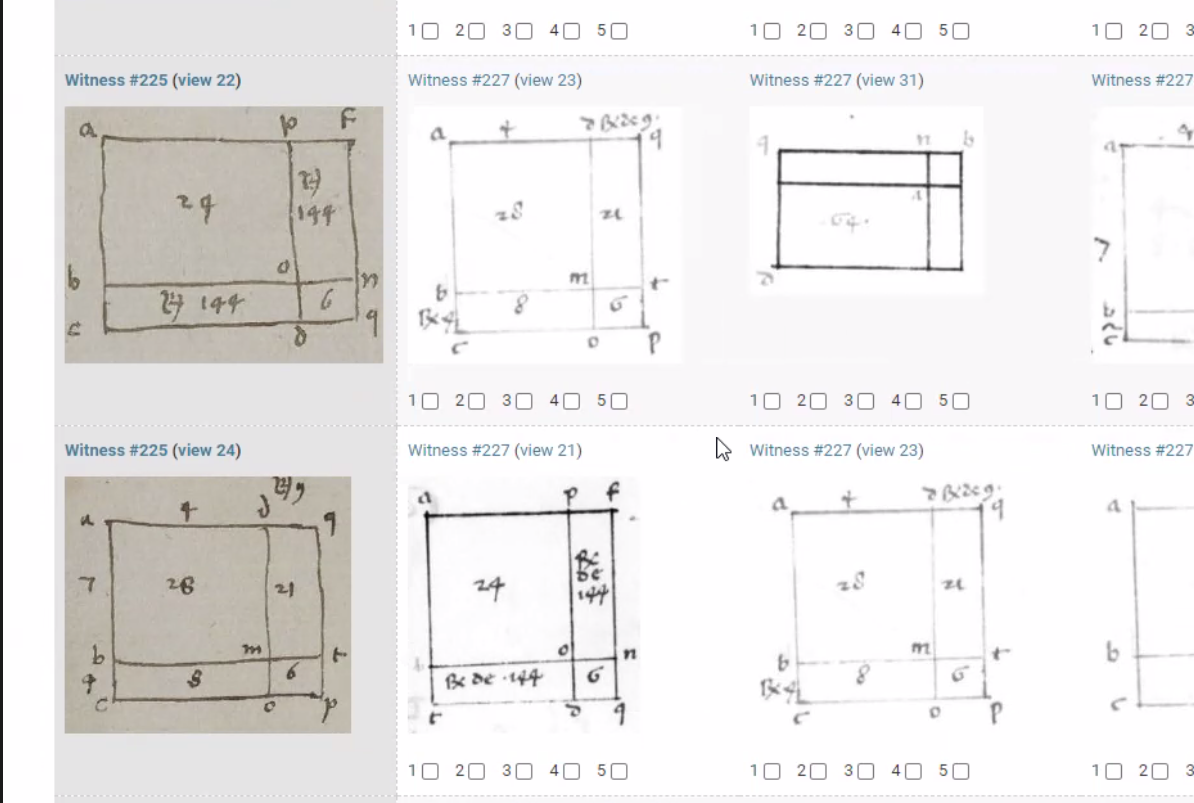
\includegraphics[height=7cm]{figues/label_dissim_exemple.png}
          \end{center}
          \caption{Impact des labels sur la recherche de similarité.}
          \label{fig:simlabel} \end{figure}

Devant ces difficultés il a été décidé d'adopter une annotation binaire
et basée uniquement sur le contenu graphique, partant du principe que
l'assignation d'un score de similarité par le modèle ne vaut pas pour
conclusion historiographique. Il sera toujours plus facile de ne pas
prendre en compte un résultat, et la visée de cet entraînement est
d'aboutir à un modèle assez extensif et généraliste. Il subsiste
cependant des dissensions au sein de l'équipe entre une définition très
stricte de la similarité, quitte à accepter des faux négatifs, et une
définition plus souple (typiquement, sensible aux labels), quitte à
créer des faux positifs. Pour concilier les besoins de tous les
chercheur.ses, il sera recommandé d'annoter selon la définition la plus
rigoureuse d'un point de vue scientifique, cette définition servant de
métadonnée aux chercheur.ses. Les annotations les plus souples seront
utilisées pour l'entraînement du modèle. Cette approche permet de
garantir une précision dans la classification des données tout en
offrant la souplesse nécessaire pour optimiser les performances des
algorithmes d'apprentissage automatique.

Ce cas d'étude est assez caractéristique des enjeux tenant à la
coordination au sein et entre des équipes de recherche dans le cadre du
développement d'un outil commun. D'où le développement des outils
d'annotation dans la plateforme commune assez généralistes pour que leur
usage s'adapte à des besoins différents et complexes\footnote{En
  réalité, les équipes de \vhs sont aussi passées à un classement binaire
  pour prévenir des problèmes de coordination au sein de leurs équipes,
  gardant l'usage des trois autres catégories pour une prochaine étape
  de fine-tuning.}.

\hypertarget{corpus}{%
\subsection{Corpus}\label{corpus}}

Les sources primaires d'\eida couvrent un spectre géographique et
temporel important. Orienté par les objectifs scientifique d'\eida --
arriver à une représentation globale des continuités et divergences qui
se tracent au cœur des pratiques astronomiques à travers l'histoire,
esquisser le voyage des sources à travers le temps et l'espace -- le
refus d'une vision eurocentrée justifie et explique une représentativité
large, servie par la constitution de cinq grands corpus issus de sphères
géographiques et temporelles diverses. Les manuscrits arabo-persans
produits entre le \textsc{viii}\ieme et le \textsc{xiii}\ieme siècle, des manuscrits latins
médiévaux produits majoritairement entre le \textsc{xiii}\ieme et le \textsc{xvi}\ieme siècle, les
manuscrits byzantins, produits entre les \textsc{ix}\ieme et \textsc{xv}\ieme siècles, les
manuscrits sanskrits, à partir du \textsc{xi}\ieme, et enfin les sources chinoises
datant du milieu du \textsc{xvi}\ieme siècle, après l'arrivée des premiers jésuites.
Le support de ces dernières n'est pas nécessairement le manuscrit, elles
prennent souvent la forme d'imprimés par blocs xylographiques dont les
matrices sont réemployées dans plusieurs témoins. Elles présentent donc
une forme hybride, sorte de pré-imprimé, qui posa des questions
complexes pour la modélisation conceptuelle des données.

Plusieurs centaines de manuscrits sont numérisés pour chaque tradition.
Sur ces numérisations, mises à disposition par les institutions
patrimoniales qui conservent ces témoins, seront appliquées les
traitements en prévision de l'analyse par les chercheur.ses, leur
permettant de souligner les motifs qui sous-tendent la diffusion
afro-eurasiens du modèle ptoléméen.

La gémellité avec \vhs impose un effort de modularité pour pouvoir
partager le modèle de données. Le travail de recherche de \vhs est mené
sur quatre corpus relevant, à l'instar de celui d'\eida d'une grande
diversité chronologique et géographique. Ces corpus se distinguent
cependant par une grande diversité thématique~: ils se composent de
manuscrits et d'imprimés concernant les sciences des mathématiques et
les sciences naturelles. Le premier corpus est le \emph{Physiologus},
rédigé vers le \textsc{ii}\ieme siècle à Alexandrie. Ce texte, l'un des plus
populaires du \ma, a contribué à l'émergence de la zoologie
chrétienne médiévale. Il a pour témoins 100 manuscrits grecs, dont treize
sont illustrés et réalisés entre le \textsc{xi}\ieme et le \textsc{xvi}\ieme siècle, contenant
environ 680 images d'animaux, de plantes et de minéraux. Le deuxième
corpus est le \emph{De materia medica} de Dioscoride, composé vers l'an
77 de notre ère. Ce traité pharmacologique destiné aux praticiens a été
largement diffusé et copié. Il est conservé dans 65 manuscrits grecs,
dont 17, réalisés entre le \textsc{vi}\ieme et le \textsc{xvi}\ieme{} siècle, sont illustrés et
contiennent environ 8340 images de plantes, d'animaux et de minéraux.
Les troisième et quatrième corpus se composent des planches de
l'Encyclopédie de Diderot et d'Alembert (1751-1772), les témoins de ce
travail couvrant une longue série de traités, dictionnaires et
encyclopédies au fil desquels les illustrations ont été copiées et
retravaillées. Leur étude se focalise aussi sur leur inclusion
ultérieure dans des encyclopédies telles que l'Encyclopédie méthodique.
Le troisième corpus se concentre sur l'Histoire naturelle (Zoologie),
tandis que le quatrième porte sur les sciences mathématiques\footcite{noauthor_vhs_nodate}.

Le deux corpus jumeaux diffèrent aussi en taille~: celui de \vhs présente plus de 2000 témoins devant 300 pour \eida.

Malgré ces divergences importantes, les données sont issus de spectres
assez larges pour opérer des croisements dont l'exploitation peut
s'avérer fructueuse~: les corpus \vhs présentent quelques diagrammes
astronomiques, et les manuscrits \eida présentent plusieurs images de
plantes. La mise en commun des résultats permet d'établir des liens
entre le \ma (focus d'\eida) et la période moderne (focus de \vhs)
pour les domaines respectifs étudiés. Notamment, des chercheur.ses d'\eida
s'intéressent à la transition du manuscrit à l'imprimé. La possible
jonction des corpus reste néanmoins problématique, et les modèles d'\ia doivent être spécialisés sur les objets d'étude respectifs des deux projets.

Ces remarques sont révélatrices de l'entre-deux qui nous intéresse dans
ce mémoire~: bien que les projets aient un objectif et des objets
d'étude précis, ceux-ci se trouvent élargis par le réseau institutionnel
et les dynamiques collaboratives qui accompagnent la création des outils
numériques. Le niveau de modularité de l'outil créé devra prendre en
compte cette généralisation possible sans perdre de vue les objectifs
initiaux des deux projets.

\hypertarget{modele-de-donnees}{%
\subsection{Modèle de données}\label{modele-de-donnees}}

L'application commune à \vhs/\eida est développée avec le \textit{framework} Django
et adossée sur une base de données gérée avec PostgreSQL. Le modèle de
données conçu pour l'application a fait l'objet de réflexions et
réadaptations pour répondre aux besoins de description des sources de
\vhs et \eida, tout en restant suffisamment flexible pour être utilisé par
d'autres projets souhaitant reproduire les méthodes employées par les
deux projets. Le défi consiste à conceptualiser la donnée de manière
suffisamment spécifique et assez généraliste.

\hypertarget{modele-initial}{%
\subsubsection{Modèle initial}\label{modele-initial}}

Le modèle de données initialement construit\footnote{Voir l'annexe \ref{data_models} pour une illustration de l'évolution du modèle de données.} pour
l'application \vhs prévoit l'existence des entités 'manuscrit' et
'imprimé', qui correspondent aux supports représentés dans
les corpus d'\eida et de \vhs. Ces deux \emph{états matériels} du texte
sont reliés à une entité plus abstraite~: le \wo.
S'appuyant sur la définition de \wo que donne le CIDOC-CRM\footnote{Le
  modèle conceptuel définit, dans un domaine donné, comment représenter
  la réalité. À ce titre il est indépendant de la manière dont on stocke
  les données informatiquement. Né dans le domaine des musées, CIDOC-CRM
  est un modèle conceptuel standardisé pour la modélisation des
  informations dans le domaine du patrimoine. Il vise à décrire et à
  rendre interopérables des objets du monde culturel en général. La
  notion d'événement se trouve au cœur du modèle, traduisant une
  approche monotonique des données~: les objets décrits peuvent évoluer,
  on peut toujours décrire de nouveaux événements liés à cet objet.
  Ainsi, on n'aura potentiellement jamais terminé de décrire un objet en
  CIDOC-CRM.}, un \wo est indépendant de sa forme matérielle, c'est une
production intellectuelle qui peut se manifester dans différentes
sources, pouvant elles-mêmes présenter des variations.

Mais ce premier modèle va rapidement montrer des limites, notamment
liées à la description d'une même œuvre divisée en plusieurs ouvrages,
ou d'un ouvrage contenant plusieurs œuvres. De plus, la pertinence de la
distinction absolue des manuscrits et imprimés ne permet pas une
description pertinente de tous les objets~: par exemple les sources
chinoises, dont le support n'est pas nécessairement le manuscrit,
prennent souvent la forme d'imprimés par blocs xylographiques dont les
matrices sont réemployée. Ces constats ont mené à la refonte de ce
modèle de données. 

\hypertarget{premiere-refonte}{%
\subsubsection{Première refonte}\label{premiere-refonte}}

Le nouveau modèle est non seulement plus pertinent mais aussi déjà plus
flexible. Il est centré autour de l'entité 'témoin' ou \wit, et
est complété par d'autre tables pour décrire la diversité des sources et
leurs différents modes d'existence. Ainsi, les séries héritent
uniquement des imprimés et les témoins héritent à la fois des
manuscrits et des imprimés. Une \ser est une édition en
plusieurs volumes d'une œuvre imprimée. Le témoin ramène à chaque volume
en tant qu'entité matérielle de référence, ou à un manuscrit. Il peut
contenir un ou plusieurs 'travaux' (\wo)~; un même \wo peut
correspondre à des séries et des témoins différents (table de relation
\textit{Content}). La table \wo inclut donc les références au lieu et à l'auteur
(clés étrangères), mais aussi l'information relative à la plage de temps
durant laquelle cette œuvre a existé physiquement (durant laquelle on
atteste l'existence de témoins). La ou les numérisations
(\digits) sont reliées au \wit et contiennent les détails sur la
source de numérisation et l'état des traitements via \iiif\footnote{Voir le \hyperlink{iiif}{Chapitre 2} sur \iiif}. Une entité Tag est utilisée comme moyen de
différencier manuscrit, imprimé ou gravure, et la table de relation
\textit{Tag\_Exemplar} fait le lien entre le témoin et les tags. La table
\textit{Role} établit des relations entre des contenus (\textit{Content}), des
\emph{séries} (\sers) et des personnes (\textit{Persons}), attribuant à
ces dernières les rôles d'auteur ou d'éditeur.

Les évolutions en cours pendant mon stage, détaillées en partie
III\footnote{Voir le \hyperlink{chapitre-7-processus-et-fonctionnalites}{Chapitre 7}}, ont nécessité de faire des choix
complexes, répondant à une double exigence \emph{a priori} paradoxale~:
une plus grande flexibilité pour intégrer de nouvelles sources de
données et une précision de description suffisante. De nouvelles
questions ont été soulevées liées à la granularité et à la cohérence
sémantique.

Ce paradoxe apparent met en lumière les défis et la complexité liés à la
modélisation de la donnée, et les transformations successives reflètent
des questionnements~: comment rendre l'application la plus universelle
possible, l'ouvrir à une large diversité de sources, sans renoncer à la
qualité de la description des sources des projets de \eida et \vhs~?
Comment, d'ailleurs, conceptualiser un modèle qui convienne aux deux
projets et leurs objectifs~? Les solutions ci-dessus décrites sont
satisfaisantes mais amenées à évoluer, montrant que la modularité se
construit sur le temps long.

\vspace{2cm}

En conclusion, \aikon est
composée de plusieurs modules applicatifs, elle est extensible et facile à maintenir (l'organisation des processus se reflétant
dans l'arborescence de fichiers), tout
en facilitant la gestion des dépendances et l'optimisation des
performances. 

 \begin{figure}[H]
	\begin{center}
		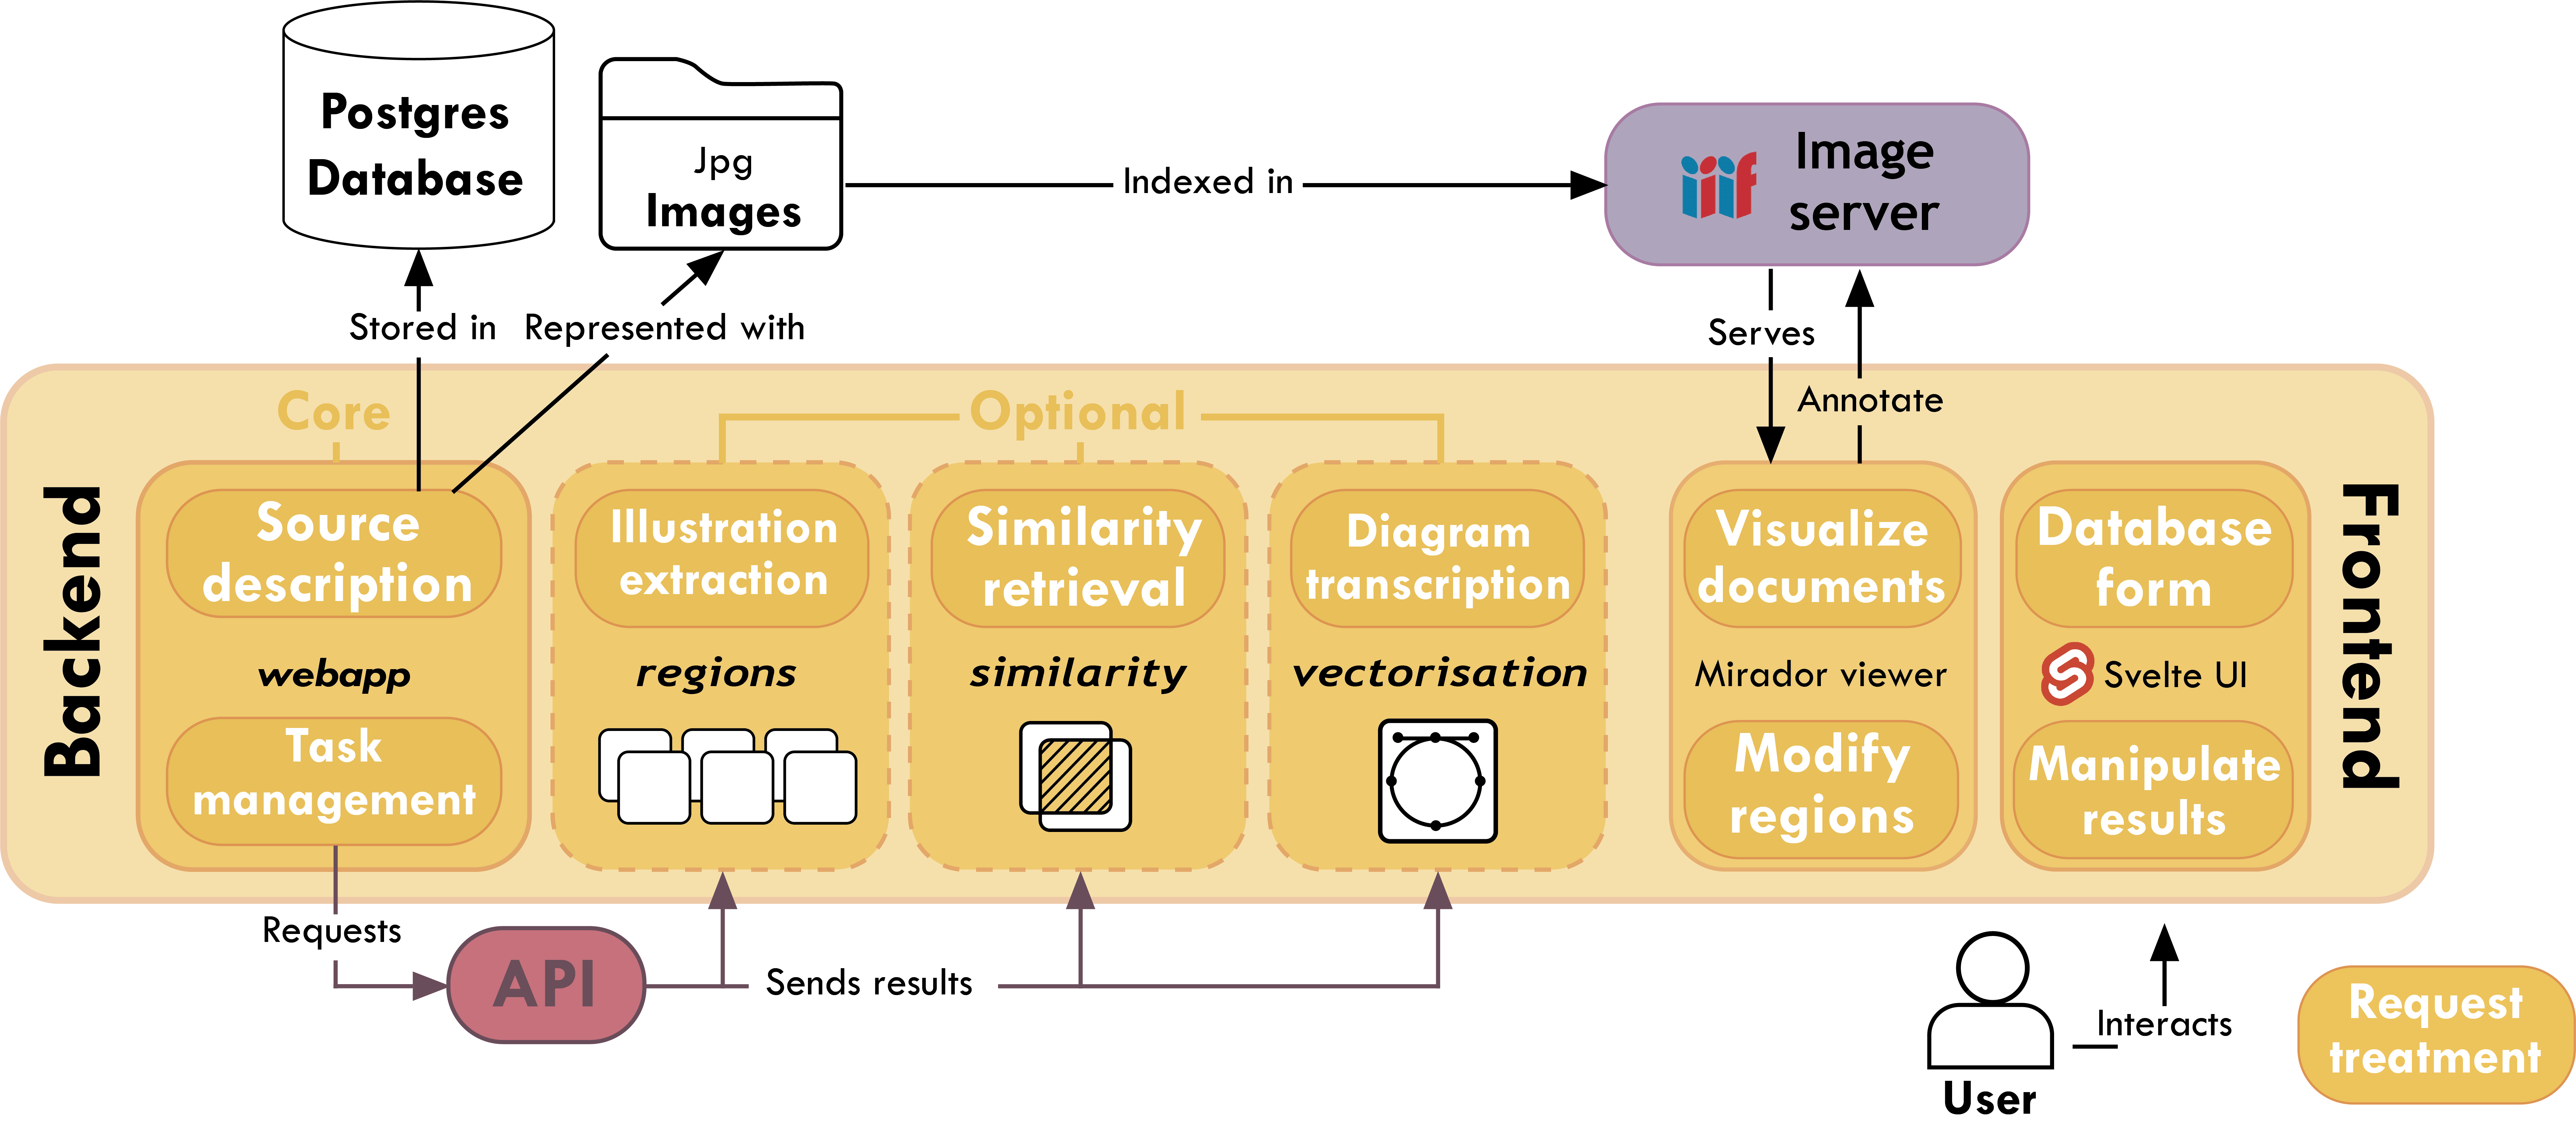
\includegraphics[height=6cm]{figues/separate.png}
	\end{center}
	\caption{Représentation schématique des fonctionnalités et processus de la plateforme.*}
	\label{fig:fonct_separes} \end{figure}

Cette approche modulaire est particulièrement bénéfique
pour les projets complexes nécessitant une collaboration entre plusieurs
équipes de développement (c'est d'ailleurs le cas dans le cadre de la collaboration \eida/\vhs), assurant la qualité et la robustesse du code,
et permet la modularité de la plateforme.
            
        \clearemptydoublepage
        
\hypertarget{chapitre-8-interfaces}{%
\chapter{Interfaces}\label{chapitre-8-interfaces}}


L'interface crée une zone d'échange et de contact entre l'application et l'utilisateur.rice, permettant d'échanger des informations grâce à l'adoption de règles communes. En cela, elle est bien plus qu'une simple couche superficielle. Elle
constitue le point de rencontre entre deux mondes~: celui de l'humain et
celui de la machine. Concevoir une interface, c'est penser à la manière
dont les utilisateur.rices vont interagir avec un système. C'est définir les
éléments visuels, les commandes, les actions possibles et la logique qui
régit ces interactions. L'interface est ainsi l'aboutissement d'un
processus de design qui vise à rendre une expérience utilisateur.rice aussi
intuitive et efficace que possible. Et, à ce titre, elle jouera un rôle
décisif dans la mise à disposition et l'adoption des méthodes d'analyse
basées sur l'\ia.

L'intégration du \dl aux pratiques des chercheur.ses en sciences
historiques peut être favorisée par le développement de la plateforme \aikon, qui leur
permet d'exploiter simplement ces outils pour traiter leurs sources.
L'interface graphique sert donc d'intermédiaire entre les chercheur.ses et les
algorithmes de vision artificielle. Elle facilite en outre le dépôt et
la gestion structurée des données sources et des métadonnées associées
et simplifie l'accès aux outils de traitement de l'images. Cette
plateforme à interface graphique doit être adaptée à une grande
diversité de documents à traiter, et pensée pour accueillir des
utilisateur.rices divers, aux compétences numériques et aux questions de
recherche variées.

\begin{kwote}
``{[}L{]}'activité de conception des plateformes digitales, chères aux
Humanités Numériques en tant que ces dernières se veulent productrices
d'outils et d'instruments, doit être considérée par nature comme
relevant d'un travail de design et, par conséquent, en intégrer la
culture créative et la philosophie dès le commencement, dans l'esprit
d'un « design des programmes » (Masure, 2014) qui doit permettre de
développer et d'améliorer le design des plateformes. Car, on le sait,
la cause principale de la réussite (et donc de l'adoption par une
communauté) d'un service numérique réside dans la haute qualité
d'expérience utilisateur.rice ( User eXperience ) qu'il est capable de
délivrer aux usagers.''\footcite{clavert_2dh_2015}
\end{kwote}

L'\ux \textit{design}, approche centrée utilisateur.rice, vise à optimiser les
interactions entre un utilisateur.rice et un système. Il s'appuie sur des
méthodes issues des sciences cognitives pour concevoir des interfaces
intuitives et efficaces. L'\ui \textit{design}, partie intégrante de l'\ux,
se concentre sur l'aspect visuel de l'interface, en cherchant à créer
une expérience esthétique et cohérente. Le projet \eida illustre
parfaitement l'importance de l'\ux/\ui \textit{design} dans le domaine de la
recherche. En plaçant l'utilisateur.rice final (le chercheur.se) au centre de
ses préoccupations, \eida vise à développer une plateforme qui le guidera
dans l'adoption des méthodes et la prise en main de la chaîne de
traitement. Ainsi un outil de recherche, pour être efficace, doit
disposer d'une interface utilisateur.rice pensée pour optimiser les \textit{workflows}
des chercheur.ses. Une bonne ergonomie, une navigation fluide et une
organisation claire des informations permettent d'assurer la cohérence
des méthodes et processus. Ainsi, l'outil pourra devenir un véritable
levier de productivité, modélisant des
processus unifiés au sein des équipes. Une interface intuitive et
agréable facilite l'apprentissage et l'utilisation de l'outil, même par
des utilisateur.rices ayant des niveaux d'expertise variés~; elle favorise
ainsi l'engagement et l'adoption, par le biais de l'outil numérique, d'une
méthodologie.

\hypertarget{faire-le-lien-avec-les-chercheur.ses}{%
\section{Faire le lien avec les
chercheur.ses}\label{faire-le-lien-avec-les-chercheur.ses}}


L'astronomie est issue d'une tradition continue vieille de près de 4000
ans qui transcende les cultures et les langues. Les théories, les
savoirs, les méthodes, au gré de leur diffusion, se mélangent aux
pratiques autochtones pour servir les usages locaux, qui bien souvent
renforcent des dynamiques de pouvoir en place, que ce dernier soit
politique ou religieux. Les sciences astrales revêtent ainsi une
importance culturelle majeure.

Une étude approfondie des sources révèle les processus par lesquels les
connaissances se sont enrichies et transformées au contact de
différentes cultures. Leur examen permet en outre de souligner les
spécificités et les innovations de chaque tradition, tout en montrant
les interconnexions et les influences réciproques qui ont façonné
l'évolution de l'astronomie. Les schémas de circulation sont dans de
nombreux cas de très grande portée géographique, chronologique et
culturelle. Ils relient des contextes de production de connaissances à
l'échelle afro-eurasienne et sur des périodes de siècles voire de
millénaires. La trace de ces transmission supporte une vision connectée
et globale de l'histoire des cultures et du savoir.

La grande diversité des sources et des approches possibles rend
cependant difficile une approche globale. À ce titre, il est important
de cibler un objet d'étude : \eida se focalise ainsi essentiellement dans
la transmission de la tradition ptoléméenne, et le corpus se compose
donc de ressources manuscrites et imprimées relevant de cette tradition.

\hypertarget{ptolemee-modele-et-transmission}{%
\subsection{Ptolémée : modèle et
transmission}\label{ptolemee-modele-et-transmission}}

Ptolémée tient une place proéminente dans l'histoire de l'astronomie et
des mathématiques. Son nom reste associé à la conception d'un système
astronomique qui plaçait la Terre immobile au centre du monde, et dont
la mise en question, de Copernic à Newton, a commandé la révolution
scientifique.

Dans sa \emph{Syntaxe mathématique}, plus connue sous le titre
d'\emph{Almageste}, et dont la dernière observation consignée date de
141, il expose l'ensemble des connaissances astronomiques de son époque.
Notamment il perfectionne le modèle élaboré par Hipparque, à qui il
emprunte la découverte de l'excentricité des trajectoires apparentes du
Soleil et de la Lune par rapport à la Terre, et l'idée de composer ces
trajectoires à l'aide de deux mouvements distincts. Il élabore un
système géocentrique au moyen d'un ensemble complexe de trajectoires
circulaires des objets pris dans un mouvement uniforme : les déférents,
autour de la Terre, et les épicycles, dont les centres parcourent les
déférents\footcite{lequeux_systeme_nodate}.

En effet, les sociétés anciennes attendent des
corps astraux (soleil, lune, planètes et étoiles) un mouvement uniforme
et le plus ``parfait'' possible, c'est-à-dire un cercle. Pourtant la
trajectoire de ces corps, observée empiriquement, n'est pas circulaire.
Le modèle de Ptolémée explique ces imperfections en postulant que les
mouvement apparemment irréguliers sont dû à cette fameuse combinaison de
plusieurs trajectoires circulaires régulières vues depuis la Terre,
point statique. Les planètes se déplacent à vitesse uniforme sur un
cercle (l'épicycle) dont le centre se déplace à vitesse uniforme sur un
cercle coplanaire (le déférent), dont la Terre est le centre.

En plus de la description du mouvement des astres, Ptolémée dresse dans
l'\emph{Almageste} des tables établissant les positions de la lune et
prévoyant les périodes et les caractéristiques des éclipses avec une
précision inédite\footcite{raymond_jones_ptolemy_2024}, un catalogue des étoiles, un traité
complet de trigonométrie plane et sphérique et une description des
instruments nécessaires à un grand observatoire.

L'œuvre de Ptolémée fera référence, et en tant que synthèse des
connaissances astronomiques antérieures, sa transmission correspond
à celle de la vision des pratiques de l'astronomie grecque à son apogée,
et sa diffusion façonnera la production astronomique ancienne pendant
près de treize siècles. D'ailleurs le nom d'Almageste date de la
transmission par les civilisations arabes à l'occident.

En effet, lors de la chute de l'Empire Romain d'occident, la majeure
partie des ouvrages antiques sont perdus et la science occidentale
stagnera jusqu'au \textsc{xii}\ieme siècle. Elle continuera cependant à progresser
ailleurs : notamment dans le monde arabe et musulman. Dès le \textsc{viii}\ieme et
\textsc{ix}\ieme siècle, les Arabes vont traduire dans leur langue la plupart des
grands textes scientifiques de l'Antiquité, en particulier les œuvres
d'Aristote et l'\emph{Almageste} de Ptolémée. Sans remettre en cause le
géocentrisme et le système de Ptolémée, ils le perfectionnent et
l'amènent à un très grand degré de précision. Nécessaire à la stricte
observation des règles de l'islam, l'astronomie arabe se développe et se
diffuse, grâce aux travaux d'al-Biruni, al-Hazen ou al-Sufi\footcite{noauthor_monde_nodate}.

À partir du \textsc{xi}\ieme et surtout du \textsc{xii}\ieme siècle, au fil des conquêtes des
occidentaux en Espagne et en Sicile, les textes grecques sont traduits
en latin via la traduction arabe. La transmission des savoirs
gréco-arabes -- notamment les traductions arabo-latines de
l'\emph{Almageste} et du Livre des étoiles fixes d'al-Sufi -- ouvre la
voie à un renouveau scientifique dans l'Occident chrétien, permettant
ainsi l'essor des grandes universités européennes de l'époque (Paris,
Oxford, Bologne, etc). On redécouvre les modèles d'Aristote et de
Ptolémée en les adaptant aux conceptions chrétiennes\footcite[``Le
  système géocentrique devient le modèle astronomique et théologique de
  l'Église, qui ne remet pas en cause la sphéricité de la Terre''][]{noauthor_monde_nodate}.

Avant l'avènement de l'astronomie grecque, les Babyloniens, dès le premier
millénaire \jc, utilisaient des calculs arithmétiques pour prévoir
la position des planètes. Ces théories ont voyagé jusqu'en Perse et en
Inde, où elles ont été adaptées et combinées à des méthodes autochtones.
Les théories grecques de l'époque de Ptolémée et de son prédécesseur
Hipparque sont également parvenues jusqu'en Inde, créant un matériel
complexe dont les influences sont difficiles à démêler. Parmi les
pratiques empruntées aux théories grecques, on relève l'emploi de termes
-- par exemple le titre du canon \emph{Romaka Siddhanta} datant du début
du \textsc{v}\ieme et qui marque les origines de la science astronomique sanskrite --
ainsi que des modèles épicycliques et des méthodes de calculs requérant
des paramètres numériques hérités d'Hipparque\footnote{\cite[p.6-7]{mercier_studies_2004} in \cite[p.15]{albouy_mediation_2019}}.

La tradition chinoise se développe de manière relativement indépendante
et les échanges ne débutent qu'autour de 200 \jc. Elle se distingue
de celle des Grecs par un intérêt plus marqué pour la prédiction
d'événements singuliers plutôt que pour les théories cosmologiques
cherchant l'établissement d'un modèle d'organisation du ciel. En effet,
en Chine impériale, l'astronomie a une fonction politique. L'empereur
est considéré comme le Fils du Ciel et ainsi la régulation du
calendrier, ou bien le succès (ou l'échec) de ses astronomes à prédire
une éclipse, se reflétaient positivement ou négativement sur lui.
L'inclusion croissante des diagrammes dans les traités après les
missions jésuites à partir du \textsc{xvi}\ieme siècle révèle l'influence des
pratiques d'Europe de l'ouest.

Pour conclure, l'\emph{Almageste} se présente donc comme une sorte
d'encyclopédie des connaissances d'une époque qui s'est enrichie avec le
temps au point de rendre difficile l'appréciation de son état originel.
Œuvre sans cesse recopiée au cours des siècles, passant du grec à
l'arabe puis au latin, transmise à travers tout le bassin méditerranéen
et dominant le \ma occidental après avoir conquis l'Islām, chaque
traduction et chaque copie de l'Almageste n'ont pas seulement transmis
son contenu, mais l'ont aussi adapté et enrichi en fonction des
contextes culturels et scientifiques de chaque époque. L'œuvre
ptoléméenne a servi de base à de nombreux commentaires et traités,
intégrant progressivement des éléments de connaissance issus de diverses
traditions scientifiques, et illustrant ainsi l'interconnexion des
savoirs à travers les civilisations.

\begin{kwote}
``Certains indices dans les manuscrits révèlent les emprunts
intellectuels qui s'opèrent au fur et à mesure des copies ; les méthodes
de calcul, le tracé des diagrammes, la mise en page des tables, la
structuration des textes techniques, la mention d'auteurs antérieurs, la
réutilisation de paramètres astronomiques ou même la récurrence de
certaines erreurs sont autant de signes qui témoignent des échanges
culturels qui ont façonné la pratique de l'astronomie.''\footcite[p.14]{albouy_mediation_2019}
\end{kwote}

Comme l'entend \citeauthor{albouy_mediation_2019}, les diagrammes font partie des révélateurs des
échanges intellectuels.

\hypertarget{le-diagramme-vecteur-de-connaissances}{%
\subsection{Le diagramme vecteur de
connaissances}\label{le-diagramme-vecteur-de-connaissances}}

L'historiographie et l'histoire des sciences n'échappent pas au récent
``visual digital turn''\footcite[``Digital humanities research has
  focused primarily on the analysis of texts. This emphasis stems from
  the availability of technology to study digitized text. Optical
  character recognition allows researchers to use keywords to search and
  analyze digitized texts. However, archives of digitized sources also
  contain large numbers of images.''][]{wevers_visual_2020} général des
humanités, montrant à quel point la production et la diffusion du savoir
croisent les représentations visuelles rendant compte de ces
connaissance. De fait, on ne s'intéresse plus seulement au texte. Or les
astronomes, au fil de l'histoire, ont eu recours à un grande diversité
de matériaux. Les sources primaires sont constituées par des instruments
et des écrits, ces derniers eux-même hétérogènes. Dans les traités
anciens, on trouve des descriptions détaillées, des propositions
mathématiques, des tables de calcul, et des diagrammes illustrant
souvent le texte qu'ils accompagnent. Les sources primaires peuvent en
outre être enrichies de commentaires et de gloses, prose ou
illustrations, témoignant de la manière dont les connaissances ont été
transmises et interprétées. Elles révèlent également les méthodes
pédagogiques employées pour enseigner ces savoirs.

Au cœur de cette diversité, le diagramme, objet hybride pour deux
raisons : il combine un contenu géométrique (des lignes, arcs et
cercles) et des labels, et il entretient un lien (plus ou moins étroit)
avec le texte qui l'accompagne.

En tant que structure de pensée, la figuration géométrique -- une forme
de création de modèles associée à l'élaboration et à la résolution de
problèmes dans divers domaines de la pensée humaine liés au calcul
abstrait et à la modélisation des idées -- est aussi ancienne que
presque toute autre forme d'enregistrement des pensées et des idées. Des
diagrammes utilisés pour calculer la superficie de parcelles et de
terres apparaissent dans le Papyrus mathématique Rhind, la source la
plus importante qui subsiste pour l'histoire des mathématiques dans
l'Égypte ancienne\footcite[p.6]{safran_diagram_2022}. Instruments
de pensée et de démonstration, ils servent non seulement à transmettre
le savoir mais aussi à le produire. Et dans un étrange mouvement
métaréflexif, ils permettent aux historien.nes des sciences de produire la
connaissance sur ces anciennes traditions heuristiques et leur
transmission.

Les diagrammes sont, pour les astronomes, le support d'une pratique
scientifique, et sont ainsi révélateurs de leurs méthodes, de leur
contexte d'exercice et de leur conception de leur discipline. Ils
revêtent des rôles et des aspects différents, permettant d'identifier
des modes diagrammatiques\footnote{La ``diagrammatisation'' désigne
  assez largement l'investissement des acteurs dans la complexification
  des représentations visuelles des propositions scientifiques présentes
  dans les traités.} spécifiques d'un lieu ou d'une époque, et traçant
des lignes de diffusion des pratiques et des savoirs.

Au \ma, trois grandes cultures coexistent en Eurasie : les
cultures byzantine, islamique, et d'Europe occidentale. Elles
connaissent des évolutions différentes en termes linguistiques et
religieux ; cette diversité est vraie également pour les usages auxquels
les diagrammes astronomiques étaient destinés, pour les domaines dans
lesquels ils étaient reconnus comme des instruments de pédagogie et des
vecteurs de pensée, ainsi que pour la place accordée à la culture
visuelle plus généralement et aux modes de représentation
diagrammatiques. Pourtant cette coexistence donne lieu à des échanges
intellectuels, artistiques, diplomatiques et commerciaux. Les
traductions d'œuvres savantes, les transferts de manuscrits illustrent
la porosité des frontières du savoir et de l'interdépendance des
cultures. Les diagrammes astronomiques sont à ce titre témoins des
chemins de diffusion des connaissance et des pratiques des sciences.

\emph{Comment ces diagrammes parlent-ils aux historien.nes ?}

Les diagrammes peuvent être étudiés intrinsèquement (quelles conventions
gouvernaient le langage visuel, quelle fonction assumaient-ils ?) ou
extrinsèquement (pour comprendre la transmission de ces traditions et
ces pratiques entre l'Europe et l'Asie, en passant pas la péninsule
arabique).

On pourrait penser que les formes et éléments visuels
utilisés pour une démonstration géométrique soient universels, qu'ils
restent les mêmes quelle que soit la date et la langue de l'explication
textuelle, le grec, l'arabe ou le latin\ldots{} Et pourtant le contexte
géographique, temporel, et les aspects matériels liés aux technologies
d'inscription changent profondément le fonctionnement et les objectifs des diagrammes,
leurs objectifs.

L'évolution des conventions graphiques en sont un exemple frappant. Par
exemple, l'axe vertical de la Terre, bien que représenté à plat sur la
page, fut conventionnellement compris comme un axe perpendiculaire à la
coupe du globe. Au fil du temps, de nouvelles conventions graphiques ont
été adoptées, et pour les lecteurs d'aujourd'hui on représenterait
sûrement le globe terrestre avec sa profondeur pour expliciter la
représentation. Citons en outre la représentation des phases lunaires,
qui a connu une évolution concernant l'association des couleurs claire
et sombre à la pleine lune et à la nouvelle lune. Si aujourd'hui on
associerait plutôt la pleine lune à un aplat de couleur claire et la
nouvelle lune à une couleur sombre, les manuscrits médiévaux byzantins
adoptent le référentiel contraire.

De même, le rôle du diagrammes est fluctuant, et va au delà du simple
support démonstratif au service du texte. Par exemple ceux des
\emph{Traités logiques} d'Aristote ont probablement circulé
indépendamment du texte, même si tout indique que les écrits les
appelaient dès le départ. Cela souligne la distinction entre le
diagramme en tant qu'objet de démonstration et de discussion complétant
une proposition d'un côté, et le diagramme en tant qu'accompagnement des
textes scolaires, qui aide à la compréhension de l'autre\footcite[p.5]{safran_diagram_2022}. Le
diagramme peut ainsi constituer la preuve et le support d'une
réinterprétation de la proposition textuelle.

Par-dessus tout, les transformations subies au fil des copies et des
réceptions sont éloquentes pour les chercheurs. Bien que les diagrammes
soient initialement conçus pour clarifier et expliquer une proposition textuelle, ils peuvent
parfois être des vecteurs de confusion (ou d'innovation). Le même diagramme d'une même
œuvre soumis à un processus constant de transformation par les scribes,
les artistes ou les lecteurs/commentateurs. 

La recherche des erreurs
transmises a ainsi un intérêt philologique important. Les cas de
méprises et les malentendus sont peut-être plus nombreux que les cas de
compréhension fidèle lors de la traversée des frontières géographiques,
culturelles, religieuses et/ou linguistiques, et l'étude des erreurs et modifications
révèle leurs aspects heuristiques, autant qu'il peut amener à
l'établissement d'un stemma\footcite{raynaud_building_2014}.

L'importance des diagrammes dans les transmissions est illustrée par l'exemple des diagrammes attribués à al-Ḥajjāj, en lien avec la transmission arabe des \emph{Éléments} d'Euclide. Bien que la traduction originale d'al-Ḥajjāj soit perdue, les diagrammes retrouvés dans divers manuscrits montrent qu'il utilisait parfois des schémas différents de ceux adoptés dans la tradition arabe ultérieure. Ces diagrammes ont probablement joué un rôle clé dans l'élaboration d'une version alternative de la géométrie euclidienne, influençant ainsi la transmission vers l'Europe via les traductions latines et hébraïques\footcite{de_young_editing_2014}.

Ainsi, au travers des variations, similarités et évolutions des
diagrammes, les historien.nes peuvent reconstruire les pratiques
scientifiques des astronomes et comprendre les contextes culturels et
sociaux dans lesquels elles s'inscrivaient. De telles études permettent
aussi de tracer la circulation des sources dans le monde entre les
différentes cultures et de comprendre comment celle-ci s'approprient le
contenu. En somme, l'évaluation de phénomènes diagrammatiques
indéniablement disparates à travers des géographies éloignées permet
d'identifier des modalités d'échanges culturels et leur impact sur la
construction du savoir scientifique.

Les travaux antérieurs sur l'illustration scientifique se concentrent
essentiellement sur des types spécifiques de diagrammes, situés dans des
contextes déterminés chronologiquement et culturellement. Un exemple de
ce paradigme est le projet précédent ALFA, qui porte sur les diagrammes
de tradition alfonsine médiévaux un regard eurocentré. Cependant, à
l'aune des remarques précédentes, il devient pressant de dépasser cette
perspective centripète en étendant la portée géographique et temporelle
des projets ; ambition rendue possible par la disponibilité des sources
primaires en ligne, permettant la construction de bases de données
d'images de grande envergure. Ainsi peut être mise en œuvre une analyse
plus inclusive et diversifiée des sources iconographiques -- notamment
les diagrammes\footcite{husson_eida_2022}.

Comme le dit Jeffrey F. Hamburger dans un plaidoyer pour une étude
comparative des diagrammes astronomique : ``Diagrames can thus be seen
not as embodiements of eternal truths, but, rather, as culturally
embedded objects''\footcite[p.7]{safran_diagram_2022}.

\begin{kwote}
``(\ldots) to be effective, a cross-cultural comparison of diagrammatic
traditions must look beyond the prima facies appearence of the diagrams
under consideration to their underlying operations and the patterns of
thoughts that they both codified and were intended to
inculcate.''\footcite[p.3]{safran_diagram_2022}
\end{kwote}         

Les interrogations soulevées par le projet \eida se déclinent donc comme
suit : analyser l'articulation entre les fonctions documentaires et
épistémiques des diagrammes au sein de l'histoire des pratiques
astronomiques, interroger l'importance des diagrammes dans la
construction et la transmission des connaissances scientifiques, et
enfin identifier des schémas récurrents dans les modalités de
circulation de ces diagrammes. S'appuyant sur ces analyses, les
chercheurs pourront à leur tour tracer des lignes : au sens figuré
construire ``a web of connections linking the points represented by the
individual contributions together into a larger pattern''\footcite[p.10]{safran_diagram_2022} ; et
au sens propre, cette vision globale sur la vie des images et des œuvres
pouvant permettre l'établissement d'éditions critiques normalisées.

\hypertarget{choix-techniques}{%
\section{Choix techniques}\label{choix-techniques}}

\gaga mène une réflexion
méthodologique sur la portabilité des modèles, leur diffusion et le
partage de grands ensembles de données annotées selon des normes
communes. Les modèles d'\ia, notamment ceux dédiés à la
reconnaissance du texte manuscrit (\htr) et au traitement automatique des
langues (\tal), requièrent des données d'entraînement spécifiques. 

Mais si chaque projet de recherche annotait ses corpus selon ses propres
exigences, ils engendreraient fatalement des silos de données non
réutilisables. Pour garantir la réutilisation des données, il est
impératif d'établir des normes et des standards.

Le projet porte alors le développement d'une syntaxe
d'annotation générique pour harmoniser la segmentation des pages des
vérités de terrain, afin de constituer des corpus d'entraînement réutilisables. \gaga propose une
approche très inclusive en identifiant des éléments textuels communs à
une large variété de documents, manuscrits comme imprimés. Cette
démarche donne lieu à la définition d'un vocabulaire contrôlé permettant
ainsi de construire des corpus annotés compatibles avec différents contextes\footcite[``Using a common vocabulary to annotate zones called SegmOnto (that is still evolving), we have developed a generic workflow to analyse the layout, OCRise the text, and convert the ALTO output into minimally encoded TEI files (\dots).''][p.2]{janes_towards_2021}~:
SegmOnto\footnote{https://github.com/SegmOnto}

Les étapes de lemmatisation et d'étiquetage morphologique (POS-tagging) effectuées par les modèles de \tal sur le texte extrait des pages numérisées visent à normaliser le
langage en réduisant les mots à leur forme canonique (lemme) et en
identifiant leur catégorie grammaticale. Cette normalisation est
essentielle pour faciliter des analyses ultérieures telles que la
collation et la stylométrie. Elle permet une analyse comparative des textes
malgré la grande variabilité inhérentes aux
langues historiques, pour lesquelles l'absence de normes orthographiques entraîne une
grande diversité de graphies. La préparation des données, là aussi, a donné lieu à une
réflexion méthodologique sur les défis liés à la standardisation des
annotations linguistiques dans les corpus diachroniques.

Selon \citeauthor{gabay_standardizing_2020}~:
\begin{kwote}                     
	``With the development of big corpora of various periods, it becomes
	crucial to standardise linguistic annotation (e.g.~lemmas, POS tags,
	morphological annotation) to increase the interoperability of the data
	produced, despite diachronic variations.''\footcite[p.2]{gabay_standardizing_2020}
\end{kwote}  

\citeauthor{gabay_standardizing_2020}\footcite{gabay_standardizing_2020} relèvent la
difficulté de mettre en œuvre un cadre technique qui prenne en compte
les pratiques d'annotation déjà établies et propres à des états de la langue. Pourtant garantir une
interopérabilité minimale avec les corpus existants est essentielle pour
maximiser la valeur ajoutée des nouvelles données.

\begin{kwote}                     
	``Such a task cannot be done without taking into account longstanding
	annotation practices, in order to allow (minimal) interoperability with
	already existing datasets. Such a statement is sadly easier said than
	done, because EMF is an intermediary stage between medieval (12th-15th
	c.) and late modern and contemporary (from c.~1750) French, two states
	of language that tend to have different needs regarding annotation: EMF
	is then caught in between two (potentially incompatible) practices, one
	for each extreme of the continuum.''\footcite[p.2]{gabay_standardizing_2020}
\end{kwote}     

Il est particulièrement complexe de trouver un équilibre entre une
description linguistique trop fine, qui pourrait limiter
la réutilisabilité des corpus, et une description trop générale, qui pourrait
manquer de précision. De plus, les besoins en annotation varient considérablement
entre le français médiéval et le français moderne, et les systèmes
d'annotation de ses deux états de la langue sont difficilement
réconciliables~: or une large partie des sources de \gaga se
situent dans l'entre-deux. Trouver un compromis qui satisfait les
exigences spécifiques de chaque période est complexe.

L'harmonisation des annotations vise à favoriser la diffusion des corpus
de données sur HTR-United, une plateforme collaborative dédiée au
catalogage de vérités de terrain pour l'\htr et l'\ocr, principalement en
français\footcite{chague_htr-united_2021}. Cette base de
données, hébergée sur GitHub, centralise des images et leurs
transcriptions produites par différents projets de recherche, offrant
ainsi une diversité de jeux de données diachroniques et géographiques
pour l'entraînement de modèles \htr.

\gaga vise aussi à la diffusion des modèles en eux-même, qui peuvent alors être réutilisés et spécialisés. Par ailleurs, le projet
s'appuie sur des outils existants, par exemple Deucalion, une boîte à
outils de traitement automatique des langues (\tal) conçue pour être
interopérable avec d'autres systèmes\footnote{https://github.com/chartes/deucalion-model-af}.

\vspace{2cm}

On aura voulu montrer dans cette section l'importance du travail des
interfaces, qui font le lien entre le chercheur.se et la donnée d'une part,
et entre le chercheur.se et des pratiques d'autre part. Plus que de simples
ornements, des interfaces performants impactent l'analyse des données,
ainsi que l'adhésion et l'efficacité des utilisateur.rices. Elles constituent
le pont entre les chercheur.ses, souvent peu familiers des bases de
données, et les données complexes qu'ils produisent. Une interface
permet de faciliter la navigation entre les sources, même si elles sont
hétérogène, et permet aux chercheur.ses de retrouver facilement les données
dont ils ont besoin, grâce à des fonctionnalités de recherche
pertinentes. L'utilisation de formulaires de saisie réduit les erreurs
et permet une gestion normalisée des métadonnées, favorisant la
trouvabilité et la réutilisation des données par d'autres chercheur.ses.
Des outils de visualisation leur permettent une exploration de leurs données centrée sur l'élément graphique, unité de base du modèle.

L'interface permet aussi de guider le chercheur.se dans un protocole.
Unifier l'accès aux données et aux modèles de vision par ordinateur
implique d'élaborer des \textit{workflows}, facilitant la mise en œuvre de méthodes standardisées. L'interface facilite leur prise en main,
favorisant ainsi la cohérence des méthodes au sein des
équipes, ou entre plusieurs équipes de recherche (à l'instar de
l'annotation des prédictions, destinées à être réutilisés pour
l'entraînement des modèles). Une interface bien conçue peut donc
faciliter notamment le travail en équipe, améliorant le partage des pratiques.

Afin de répondre à ces exigences, le travail de front est clé. La
plateforme \aikon a été pensée pour proposer des interfaces performantes pour les fonctionnalités de recherche et de visualisation diverses. Ce travail pour rendre
la plateforme réactive et accueillante anticipe en outre la valorisation et la médiation des données de la recherche vers un public plus large (via la construction d'une plateforme
publique). Les choix techniques sont faits dans ce sens, l'utilisation
d'un \textit{framework front-end} permettant d'améliorer les performances et de
garantir une fluidité d'interaction, tandis que l'adoption d'un
\textit{framework CSS} assure une uniformité et une cohérence visuelle, dotant la
plateforme d'une identité graphique forte.

        \clearemptydoublepage

        \chapter*{Conclusion partielle}

Le travail des chercheur.ses sur de grandes quantités de données
nécessitent le développement d'outils adaptés. La performance des
modèles d'\ia ne suffit pas~: il faut les rendre opérationnels au sein
des environnements de recherche. Là se situe l'enjeu de la plateforme
\aikon, dont l'objectif est de rendre compatibles les outils techniques
et les pratiques des ss. Elle a pour ambition de façonner un
véritable \si incluant les outils de \cv pour
systématiser les traitements, des fonctionnalités de gestion
documentaire, le tout en préservant le rôle central de l'interprétation
humaine.

L'objectif est aussi de concevoir une plateforme adaptable à une
multitude de projets de recherche en études visuelles. En adoptant une
architecture modulaire, divers projets peuvent l'exploiter comme une
`coquille', en personnalisant les protocoles selon leurs besoins
spécifiques. Cette flexibilité contribue à la pérennité et l'évolution
de l'outil.

À l'heure actuelle, l'application est à déployer sur des serveurs
personnels. Cependant, l'objectif à long terme est de développer une
plateforme en ligne, à l'exemple d'e-Scriptorium, dédiée à l'analyse
automatique de documents multimodaux. En offrant des fonctionnalités de
correction des traitement et d'exploration de résultats, elle permettra
la création de corpus enrichis. Et en rationalisant les méthodes de
travail des historiens, elle ouvrira de nouvelles perspectives en
matière de collaboration et de partage des outils comme des données. Se
conformant aux principes \fair et aux normes internationales d'interopérabilité, elle pourra faciliter la migration des données vers
d'autre systèmes (via des \api), et permettre ainsi les
comparaisons avec d'autres corpus. Elle favoriserait ainsi son intégration
dans des écosystèmes de recherche plus larges.

\clearemptydoublepage
    
    \chapterNo{Conclusion}
    \addcontentsline{toc}{chapter}{Conclusion}
    \begin{kwote}
``Les outils façonnent la pensée. Ce que nous pouvons penser et ce que nous pouvons dire résulte d’une dynamique dans laquelle les outils et les techniques jouent un rôle fondamental.''\footcite[p.31]{epron_ledition_2018}
\end{kwote}

\citeauthor{epron_ledition_2018} avancent l'idée selon laquelle les outils ne sont pas de simples instruments passifs, mais des acteur dans la construction de la pensée. Ils ne se limitent pas à faciliter des tâches, mais façonnent une conceptualisation du monde et des idées. Les outils de la recherche, qu'ils soient numériques ou analogiques, structurent des gestes intellectuels. Les outils numériques ne sont pas de simples remédiations des outils traditionnels. Ils offrent de nouvelles possibilités, de nouvelles façons d'interagir avec l'information et de la manipuler. Ils peuvent catalyser les dynamiques collaboratives autour de ces nouvelles méthodes et ces nouvelles perceptives. Un cadre technique contient un cadre conceptuel, et il y a donc un enjeu à forger des outils de traitement de la donnée qui vont dans le sens du partage des pratiques.

Ce travail s'est attaché à exposer l'importance et les moyens de partager le développement et l'utilisation des outils numériques de la recherche, en prenant pour exemple l'application du \dl à la sémantification et l'enrichissement des sources en histoire de l'astronomie. Les questionnements, impliquant la modélisation, l'accès à la donnée, et l'élaboration des modèles de \cv, s'orientent vers la conception d'un \si dédié à des documents numérisés variés et hétérogènes, et au traitement de leurs éléments visuels. Les outils de \dl sont mis à disposition via une plateforme web modulaire et réemployable dans différents contextes (\aikon).

La première partie de ce mémoire, qui portait sur le contexte disciplinaire des projets \eida/\vhs, a mis en évidence la complexité des données traitées, ainsi que la diversité des besoins des chercheur.ses. En conséquence, une modélisation de données flexible et interopérable, ne renonçant pas aux exigences de description des sources, a constitué un axe de réflexion. Par ailleurs, la variété des modes d'accès aux données est une piste d'analyse importante. Les données visuelles et les besoins spécifiques des historien.nes, notamment l'accès à leurs propres images stockées localement, nécessitent des solutions techniques adaptées. Bien que \iiif offre un cadre prometteur pour l'échange de données volumineuses, il ne constitue pas une solution universelle.

Dans un second temps, nous avons présenté sur les enjeux et défis liés à l'utilisation du \dl et de la \cv dans le traitement des données historiques, notamment les moyens de gérer la faible disponibilité de corpus annotés. Nous nous sommes ensuite penché sur une application des traitements d'\ia, en dressant les exigences fonctionnelles d'un outil d'édition des \svgs (sorties de l'algorithme de vectorisation) intégré à la plateforme. Cet outil a vocation à fédérer les pratiques des chercheur.ses pour l'édition des diagrammes astronomiques. 

La troisième partie est consacrée aux spécificités techniques de la conception d'une plateforme modulaire destinée à héberger les outils de gestion de données et les instruments de \cv. Cette plateforme présente une architecture modulaire, reposant sur une séparation claire des fonctionnalités dans des modules et des composants applicatifs distincts. L'inférence des modèles, qui exige une puissance de calcul importante, est optimisée par l'utilisation d'un \gpu sur lequel tourne une \api prévue à cet effet. Par ailleurs, le choix d'une bibliothèque \textit{front-end} permet de créer des interfaces utilisateur.rice performantes, facilitant ainsi l'interaction des chercheur.ses avec un processus de travail itératif, alternant phases de traitement par les modèles de vision et corrections afin de garantir la qualité des résultats. Ces derniers constituent des corpus annotés qualitatifs qui pourront être réutilisés dans le cadre de l'entraînement des modèles. 

\textit{La modularité des outils~: pourquoi~?} 

Cette étude de cas a montré l'importance de l'accessibilité et du partage au sein de la communauté de la recherche, non seulement des données, mais aussi des outils qui vont permettre de les traiter. Cette démarche favorise à la fois l'évolutivité et la pérennité des outils numériques, permet d'établir des pratiques communes au sein de la communauté scientifique et, enfin, démocratise l'accès à des outils innovants qui ouvrent de nouvelles perspectives d'analyse des sources.

Les outils taillés trop spécifiquement sur un projet ou sur une question de recherche sont fragiles. Leur cycle de vie est intimement lié aux financements, ce qui les expose à l'obsolescence dès lors que les ressources s'épuisent. De tels développements, souvent coûteux en temps et en moyens (financiers comme humains), ne garantissent pas la pérennité des outils. Pour assurer leur survie et favoriser leur évolution, il est alors intéressant de s'inscrire dans des projets collaboratifs, et en conséquence, d'adopter une approche modulaire. En fédérant les efforts et en mutualisant les ressources, il est possible non seulement de stimuler l'innovation mais aussi de garantir la maintenance à long terme de ces outils, les rendant ainsi plus robustes et pérennes.

L'ouverture des outils et l'extensivité des chaînes de traitement des données a aussi des implications scientifiques d'importance. Ces aspects inscrivent une démarche scientifique dans l'optique de la collaboration et du partage des pratiques, favorisant leur reproductibilité, et renforçant la transparence des méthodes. On l'aura évoqué dans le \hyperlink{chapitre-6-vers-edition}{chapitre 6}, la diversité des pratiques d'édition scientifique des diagrammes présents dans les traités d'histoire des sciences témoigne de la richesse des points de vue sur les sources, mais peut aussi constituer un obstacle à la coopération au sein du champ de recherche. La multiplication des outils, des méthodologies et des normes entraîne une fragmentation des pratiques et remet en question l'utilité scientifique des contenus produits. Chaque chercheur.se ou chaque équipe développe ses propres outils, avec ses propres formats, et ses normes adaptées à leur angle d'approche épistémologique et heuristique. Devant ce constat, l'élaboration d'un outil d'édition numérique peut alors porter un cadre de travail partageable. 

S'adapter à l'hétérogénéité des données et des contextes matériels ne favorise pas seulement la collaboration et la cohérence des pratiques au sein d'un champ de recherche, mais facilite également l'accès aux outils d'\ia pour l'analyse à grande échelle des corpus, ouvrant ainsi de nouvelles perspectives sur les sources.

La plateforme \aikon et son interface charpentent alors un véritable environnent de recherche numérique, dédié à l'analyse des sources, orienté vers l'interprétation par les chercheur.ses. En centralisant les ressources et en offrant des fonctionnalités d'annotation et de visualisation, cet outil fait office de nouveau laboratoire, et change la manière dont les chercheur.ses interagissent avec les données historiques, permettant au domaine des études visuelles d'exploiter le paradigme du \textit{big data}. Elle est conçue pour s'adapter au traitement de documents numérisés divers, pour exploiter les éléments graphiques qu'ils contiennent.

\textit{Un outil généraliste et adaptable à plusieurs projets de recherche~: comment~?}

Le cas \aikon a en outre permis d'identifier les principaux enjeux liés à la mise en œuvre de la modularité. Nous nous sommes interrogés sur les fondements d'un outil suffisamment polyvalent et offrant une base solide pour permettre sa spécialisation.

Premièrement, la modélisation de la donnée est un aspect à considérer. Se référer à des modèles conceptuels standards est alors essentiel pour disposer de concepts larges et adaptables aux données du patrimoine. Si le modèle de données adopté n'est pas taillé spécifiquement pour décrire les source de \eida, il est néanmoins suffisamment précis pour répondre aux besoins actuels des chercheur.ses, et bénéficie de sa généralité pour s'adapter aux sources de \vhs et à une grande diversité de types de documents, permettant l'étude des éléments graphiques qu'ils contiennent. 

Le domaine de recherche de la \cv, dans son essence même, illustre en outre les dynamiques collaboratives dans la construction des instruments de traitement de la donnée. En partant de modèles génériques pré-entraînés, il est possible de construire des architectures complexes spécialisées sur des tâches et des données particulières. Pour assurer la cohérence et la réutilisabilité des données, il est important d'encourager l'utilisation de vocabulaires contrôlés et de normes pour l'annotation des données.

Une attention particulière a été portée aux interfaces de la plateforme \aikon, pour faciliter le travail des chercheur.ses et la diffusion de données. Un outil doté d'une interface graphique accueille un vaste éventail d'utilisateur.rice et anticipe en outre la médiation des résultats des recherches vers un public plus large. 

D'autre part, le recours à des protocoles standards et interopérables, tels que le \iiif, assure la compatibilité des systèmes. Les formats de sortie des traitements sont aussi des formats libres et manipulables~: \textsc{txt}, Numpy ou \svg. 

La personnalisation s'exprime par ailleurs dans le fait qu'\aikon peut être déployée dans différents environnements matériels, la possibilité d'installation en locale démontrant sa légèreté et sa portabilité. Mais les problématiques liées à l'ouverture et la modularité du code concernent aussi la conception d'une architecture qui puisse s'adapter à une augmentation du volume de données et du nombre d'utilisateur.rices. Ainsi les besoins côté ingénierie vont parfois rentrer en conflit avec cette volonté de légèreté si importante pour inclure un maximum de contextes de recherche et d'utilisateur.rices différents. La gestion de volumes de données croissants ou des outils d'\ia plus lourds requiert du matériel et des architectures applicatives plus robustes que celles développées avec les moyens des laboratoire de recherche en \shs. Pour l'instant, \aikon est taillé pour -- et utilisé sur -- des corpus qui, bien que larges, restent limités comparés aux collections des bibliothèques par exemple. Un passage à l'échelle reposerait sur l'implication de consortiums ou d'institutions, qui disposent des technologies et des infrastructures capables de gérer de grandes quantités de données de manière efficace. Nous conclurons et ouvrirons sur cette idée~: la recherche constitue le terreau de l'innovation~; néanmoins, son passage à l'échelle institutionnelle exige des compétences en ingénierie qui transcendent ceux des projets de recherche, même collaboratifs.
    

\appendix
    \part*{Annexes}	
    \addcontentsline{toc}{part}{Annexes}
    
    \chapter[Évolution du modèle de données]{\label{data_models}Évolution du modèle de données}
	    \section{Modèle de données initial de l'application VHS}
	\begin{figure}[H]
		\centering
		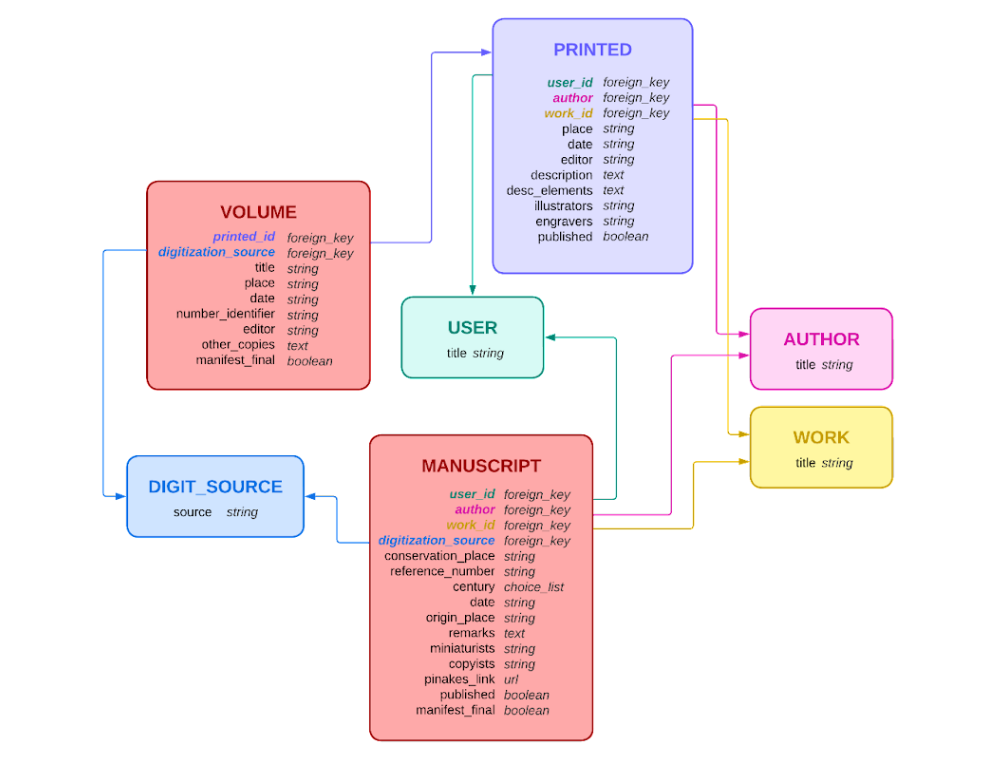
\includegraphics[width=16cm]{figues/vhs_data_model.png}
		\caption{Modèle de données de l'application \vhs avant refonte.*}
		\label{fig:vhs_data_model}
	\end{figure}

\section{Modèle de données de l'application VHS/EIDA}
	\begin{figure}[H]
		\centering
		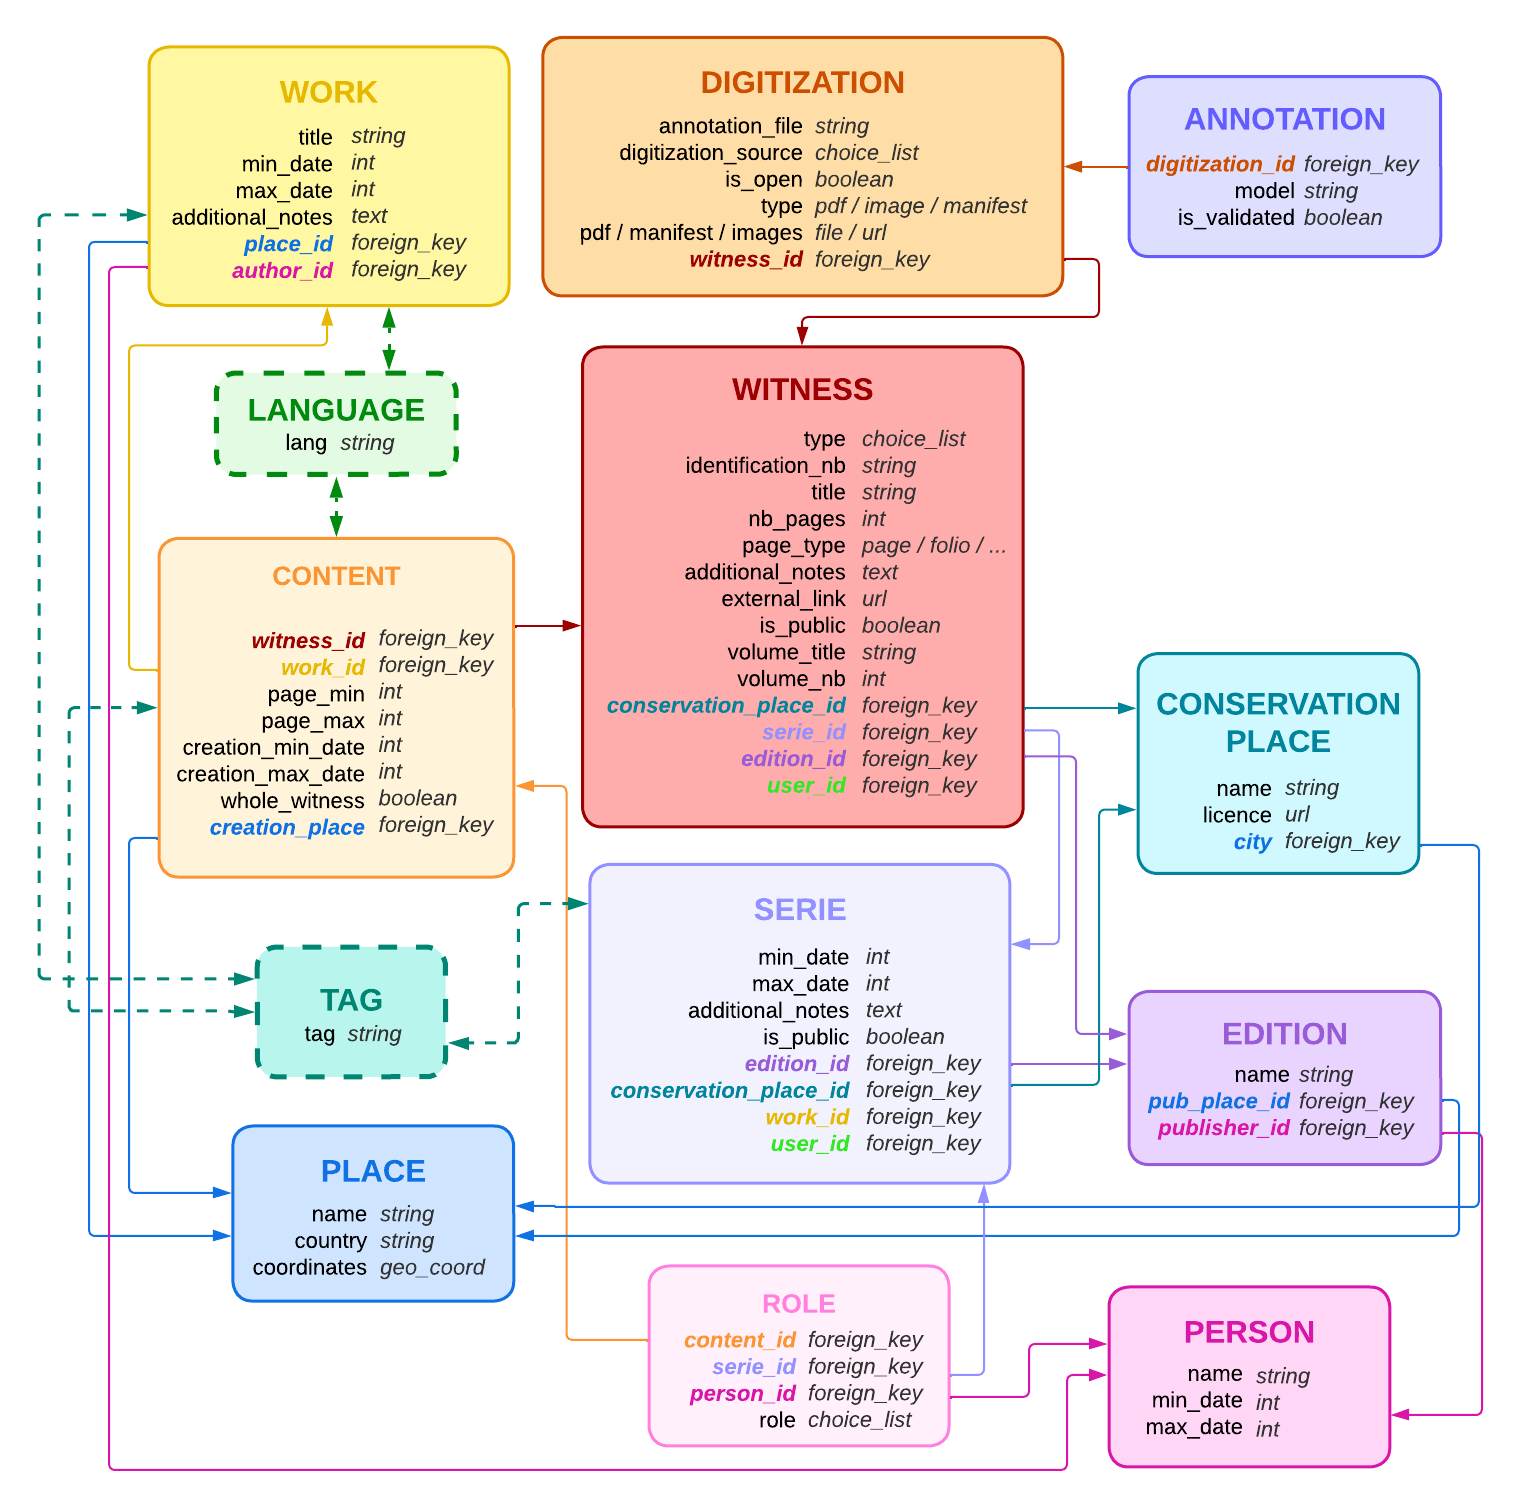
\includegraphics[width=16cm]{figues/new_model.png}
		\caption{Nouveau modèle de données de \eida appliqué à \vhs.*}
		\label{fig:eida_data_model}
	\end{figure}

 \section{Modèle de données de l'application AIKON}
	\begin{figure}[H]
		\centering
		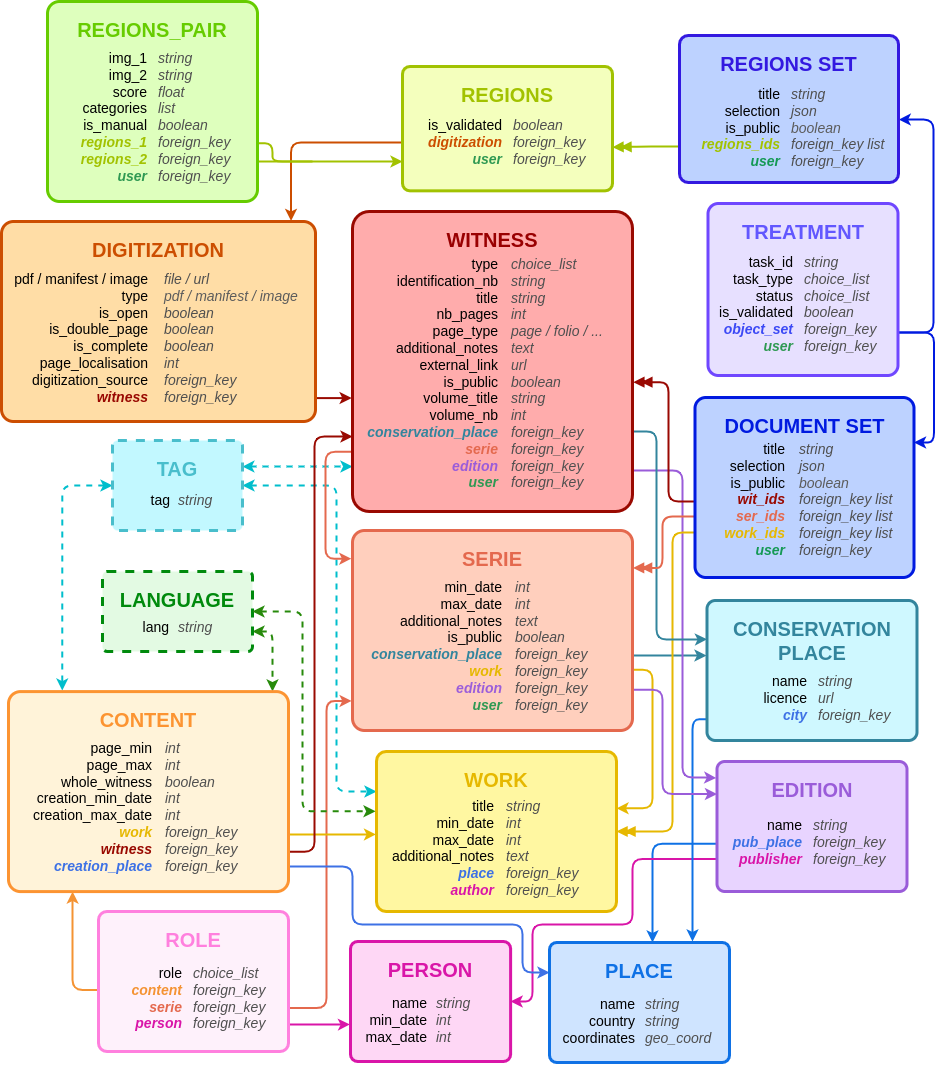
\includegraphics[width=16cm]{figues/model_aikon.png}
		\caption{Nouveau modèle de données en vue de la refonte de l'application \aikon.*}
		\label{fig:aikon_model}
	\end{figure}

 
	    \clearemptydoublepage
	
    \chapter[Module vectorisation~: description des développements]{\label{module_vecto}Module vectorisation~: description des développements}
	    Les méthodes développées pendant mon stage ont posé les bases d’un \textit{workflow}, qui a très rapidement évolué. Ces méthodes ont ensuite été itérativement raffinées pour orienter la plateforme vers plus de modularité, notamment grâce à l'implémentation de l'instance \tr, sur laquelle repose désormais le lancement des actions. Cette annexe présente le développement du \textit{workflow} de lancement de la vectorisation les \wits, ainsi que son évolution.  

\section{Workflow}
	\begin{itemize}
    \item Requête utilisateur.rice dans l’application \aikon~;
    \item Lancement d'un \tr~:
    \begin{itemize}
        \item Identification des \wits~;
        \item Parser les \mans et ramener les \URLs des régions d'images dans une liste~;
        \item Création d'un fichier \json 
        \item Envoie du \json via requête \http POST à l’\api \textit{endpoint}~;
    \end{itemize}
    \item Inférence du modèle dans Discover-Demo~: 
    \begin{itemize}
        \item Vérification du \json~; 
        \item Lancement d'une tâche~; 
        \item Enregistrement des images~;  
        \item Inférence avec le modèle~: écriture des fichiers \svgs~; 
        \item Envoi d’un \textsc{zip} contenant les fichiers à l'application via requête \http POST~;
    \end{itemize}
    \item Récupération du \textsc{zip} au \textit{endpoint} de l’application~;
    \begin{itemize}
        \item Dézip, lecture et écriture des \svgs en \textit{backend} dans l’application \aikon~;
        \item Vérification dans le répertoire de résultats (dossier dans \texttt{mediafiles}) que deux fichiers du même nom n’existent pas~;
        \item S’il existe déjà un fichier du même nom, il est écrasé par le nouveau~;
    \end{itemize}
    \item Apparition des visualisations dans l'interface~;
\end{itemize}

\section{Settings}

	\subsection{AIKON}
	
Le fichier de configuration (\texttt{.env}) de l'application doit contenir l'\URL de l'\api à laquelle elle se connecte. Afin d'activer les fonctionnalités de vectorisation, il est aussi nécessaire de spécifier le module correspondant dans les paramètres de configuration.  

	\begin{lstlisting}[language=python, frame=single, breaklines=true, caption={Extrait du fichier de configuration de l'application.}]
# Computer vision apps to install
ADDITIONAL_MODULES=regions,similarity,vectorization
 \end{lstlisting}


	\subsection{Discover-Demo}
	
Dans le fichier \texttt{.env}, la variable \texttt{INSTALLED\_APPS} contient la liste des modules à charger. Pour activer les fonctionnalités, notamment la vectorisation, il est nécessaire d'ajouter les modules correspondants à cette liste.
	
	\begin{lstlisting}[language=python, frame=single, breaklines=true, caption={Extrait du fichier de configuration de l'\api.}]
# apps (folder names) to be imported to the API
INSTALLED_APPS=dticlustering,watermarks,similarity,region,vectorization\end{lstlisting}

\section{Envoi d'un traitement de vectorisation}

\subsection{Initialisation de la requête}

Le processus de vectorisation était initialement déclenché via l'interface d'administration Django, en utilisant le mécanisme des \texttt{@admin.action} (des fonctions appelées avec une liste d’objets sélectionnés depuis la page de liste pour modification, elles agissent donc au niveau du témoin). Cette approche, bien que fonctionnelle, présentait des limites~: notamment concernant le suivi des traitements et leur application sur différents objets de la base.

Une refonte des processus a été entreprise par Jade Norindr, Ségolène Albouy et Fouad Aouinti. Cette évolution a conduit à la création d'un formulaire dédié au lancement de tous les traitements, standardisant ainsi les modes de communication avec l'\api. Ce formulaire, accessible depuis l'interface utilisateur.rice, permet d'appliquer le traitement sur un ensemble d'objets précédemment sélectionnés. 

	\begin{figure}[h]
	\centering
	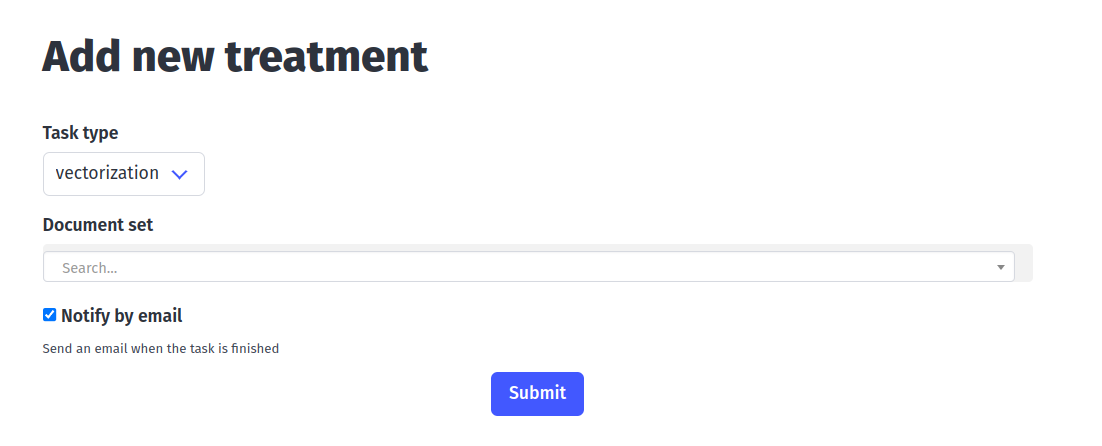
\includegraphics[width=15cm]{figues/form_traitement.png}
	\caption{Capture d'écran du formulaire d'envoi d'un traitement dans \aikon.}
	\label{fig:eida_send_manifest}
	\end{figure}

Le lancement de la vectorisation se fait donc désormais au niveau de l'entité \tr reliée à un ensemble de témoins. Le formulaire de lancement permet de créer une instance de cette entité, et par conséquent, tous les témoins associés seront soumis au processus de vectorisation.

\subsection{Création du \textsc{json}}

Initialement la fonction utilitaire \texttt{vectorization\_request\_for\_one} était utilisée pour formater un fichier \json à envoyer au \textit{endpoint} de l'\api. Afin de traiter par lots un ensemble de témoins, la fonction \texttt{vectorization\_request} permettait d'itérer sur une liste de témoins, en appelant récursivement la fonction \texttt{vectorization\_request\_for\_one} pour chacun d'entre eux.

\begin{lstlisting}[language=python, frame=single, breaklines=true, caption={Extrait de la fonction gérant l'envoi de \json à l'\api dans \texttt{app/vectorization/utils.py}}]
try:
	response = requests.post(
	url=f"{CV_API_URL}/vectorization/start",
	json={
		"doc_id": regions.get_ref(),
		"model": f"{VECTO_MODEL_EPOCH}",
		"images": get_regions_urls(regions),
		"callback": f"{APP_URL}/{APP_NAME}/get-vectorization",
		},
	)
\end{lstlisting}

Avec les récents développements, le \json utilisé pour communiquer avec l'\api est généré par la fonction \texttt{prepare\_request}, présente dans le fichier \texttt{utils.py} de chaque module. 

La boucle externe itère sur les \wits et vérifie qu'il n'y a pas déjà de vectorisation effectuée. La boucle interne itère sur les annotations des \wits. Le dictionnaire \texttt{regions\_dic} est créé pour mapper les références des témoins annotés aux \URLs des annotations. La fonction renvoie un dictionnaire contenant les données nécessaires pour la requête de vectorisation.

\begin{lstlisting}[language=python, frame=single, breaklines=true, caption={Structurer les \URLs de régions d'images.}]
def prepare_request(witnesses, treatment_id):
    regions_list = []
    regions_dic = {}

    try:
        for witness in witnesses:
            if witness.has_vectorization():
                log(
                    f"[vectorization_request] Witness {witness.get_ref()} already has vectorizations"
                )
                pass
            else:
                regions_list.extend(witness.get_regions())

        if regions_list:
            for regions in regions_list:
                regions_dic.update({regions.get_ref(): get_regions_urls(regions)})

            return {
                "experiment_id": f"{treatment_id}",
                "documents": regions_dic,
                "model": f"{VECTO_MODEL_EPOCH}",
                "callback": f"{APP_URL}/{APP_NAME}/get-vectorization",  # URL to which the SVG zip file must be sent back
                "tracking_url": f"{APP_URL}/{APP_NAME}/api-progress",
            }

        else:
            return {
                "message": f"No regions to vectorize for all the selected {WIT}es"
                if APP_LANG == "en"
                else f"Pas de regions à vectoriser pour tous les {WIT}s sélectionnés"
            }

    except Exception as e:
        log(
            f"[prepare_request] Failed to prepare data for vectorization request",
            e,
        )
        raise Exception(
            f"[prepare_request] Failed to prepare data for vectorization request"
        )
	\end{lstlisting}
 
La fonction reçoit une liste de \wits, générée par une tâche appelée par une méthode \texttt{post\_save} de l'instance de \tr~:

\begin{lstlisting}[language=python, frame=single, breaklines=true, caption={Méthode \texttt{post\_save du \tr.}}]
# vhs/app/webapp/models/treatment.py
@receiver(post_save, sender=Treatment)
def treatment_post_save(sender, instance, created, **kwargs):
    if created:
        get_all_witnesses.delay(instance)
\end{lstlisting}


\begin{lstlisting}[language=python, frame=single, breaklines=true, caption={Ramener tous les \wits à partir des entités reliées aux \tr et lancer de la tâche.}]
# vhs/app/webapp/tasks.py
@celery_app.task
def get_all_witnesses(treatment):
    try:
        witnesses = treatment.get_witnesses()
        treatment.start_task(witnesses)
    except Exception as e:
        treatment.on_task_error(
            {
                "error": f"Error when retrieving documents from set: {e}",
                "notify": treatment.notify_email,
            },
        )
\end{lstlisting}

\section{Discover-Demo~: module vectorization}

\subsection{Réception à l'\emph{endpoint} de l'API~:}

L'\emph{endpoint} (dans \texttt{api/app/vectorization/routes.py}) sert de passerelle pour lancer la tâche de vectorisation. Il valide la requête entrante, extrait les paramètres nécessaires et transfère la tâche au processus en arrière-plan pour son exécution. 

 \begin{lstlisting}[language=python, frame=single, breaklines=true, caption={\emph{Endpoint} \texttt{start\_vectorization}.}]

@blueprint.route("start", methods=["POST"])
@shared_routes.get_client_id
@shared_routes.error_wrapper
def start_vectorization(client_id):
    """
    A list of images to download + relevant data
    """
    if not request.is_json:
        return "No JSON in request: Vectorization task aborted!"

    json_param = request.get_json()
    console(json_param, color="cyan")

    experiment_id = json_param.get("experiment_id")
    documents = json_param.get("documents", {})
    model = json_param.get("model", None)

    notify_url = json_param.get("callback", None)
    tracking_url = json_param.get("tracking_url")

    return shared_routes.start_task(
        compute_vectorization,
        experiment_id,
        {
            "documents": documents,
            "model": model,
            "notify_url": notify_url,
            "tracking_url": tracking_url,
        },
    )
 
	\end{lstlisting}

 \subsection{Configuration de la tâche de fond}

Dans le fichier \texttt{api/app/vectorization/tasks.py}, la fonction \texttt{compute\_vectorization} définit un acteur Dramatiq qui exécute la tâche de vectorisation en \textit{background}. Elle initialise une nouvelle instance de la classe \texttt{LoggedComputeVectorization}, en lui passant le logger et les paramètres fournis. Elle appelle la méthode \texttt{run\_task} sur l'objet créé, qui va lancer le processus. 

 \begin{lstlisting}[language=python, frame=single, breaklines=true, caption={Tâche \texttt{dramatiq} \texttt{compute\_vectorization}.}]
@dramatiq.actor(time_limit=1000 * 60 * 60, max_retries=0, queue_name=VEC_QUEUE)
def compute_vectorization(
    experiment_id: str,
    documents: dict,
    model: str,
    notify_url: Optional[str] = None,
    tracking_url: Optional[str] = None,
    logger: TLogger = LoggerHelper,
):
    """
    Run vecto task on lists of URL
    """
    vectorization_task = LoggedComputeVectorization(
        logger,
        experiment_id=experiment_id,
        documents=documents,
        model=model,
        notify_url=notify_url,
        tracking_url=tracking_url
    )
    vectorization_task.run_task()

	\end{lstlisting}

 \subsection{inférence avec le modèle}

La classe \texttt{LoggedComputeVectorization} gère les processus de vectorisation en utilisant les paramètres fournis. La méthode \texttt{run\_task} lance sur l'instance le téléchargement des données, l'inférence du modèle, le traitement des résultats (renvoi des \svgs sous forme de \textsc{zip}) et la notification, avec journalisation tout au long du processus.

Dans le fichier \texttt{api/app/vectorization/lib/vectorization.py}~: 

 \begin{lstlisting}[language=python, frame=single, breaklines=true, caption={Classe \texttt{ComputeVectorization}.}]
 class ComputeVectorization:
    def __init__(
        self,
        experiment_id: str,
        documents: dict,
        model: Optional[str] = None,
        notify_url: Optional[str] = None,
        tracking_url: Optional[str] = None,
    ):
        self.experiment_id = experiment_id
        self.documents = documents
        self.model = model
        self.notify_url = notify_url
        self.tracking_url = tracking_url
        self.client_id = "default"
        self.imgs = []

    def run_task(self):
        pass

    def check_dataset(self):
        if len(list(self.documents.keys())) == 0:
            return False
        return True

    def task_update(self, event, message=None):
        if self.tracking_url:
            send_update(self.experiment_id, self.tracking_url, event, message)
            return True
        else:
            return False


class LoggedComputeVectorization(LoggingTaskMixin, ComputeVectorization):
    def run_task(self):
        if not self.check_dataset():
            self.print_and_log_warning(f"[task.vectorization] No documents to download")
            self.task_update("ERROR", f"[API ERROR] Failed to download documents for vectorization")
            return

        error_list = []

        try:
            for doc_id, document in self.documents.items():
                self.print_and_log(
                    f"[task.vectorization] Vectorization task triggered for {doc_id} !"
                )
                self.task_update("STARTED")

                self.download_dataset(doc_id, document)
                self.process_inference(doc_id)
                self.send_zip(doc_id)

            self.task_update("SUCCESS", error_list if error_list else None)

        except Exception as e:
            self.print_and_log(f"Error when computing vectorizations", e=e)
            self.task_update("ERROR", "[API ERROR] Vectorization task failed")

    def download_dataset(self, doc_id, document):
        self.print_and_log(
            f"[task.vectorization] Dowloading images...", color="blue"
        )
        for image_id, url in document.items():
            try:
                if not is_downloaded(doc_id, image_id):
                    self.print_and_log(
                        f"[task.vectorization] Downloading image {image_id}"
                    )
                    download_img(url, doc_id, image_id)

            except Exception as e:
                self.print_and_log(
                    f"[task.vectorization] Unable to download image {image_id}", e
                )

    def process_inference(self, doc_id):
        model_folder = Path(MODEL_PATH) 
        model_config_path = f"{model_folder}/config_cfg.py" 
        epoch = DEFAULT_EPOCHS if self.model is None else self.model
        model_checkpoint_path = f"{model_folder}/checkpoint{epoch}.pth"
        args = SLConfig.fromfile(model_config_path)
        args.device = 'cuda'
        args.num_select = 200

        corpus_folder = Path(IMG_PATH)
        image_paths = glob.glob(str(corpus_folder / doc_id) + "/*.jpg")
        output_dir = VEC_RESULTS_PATH / doc_id
        os.makedirs(output_dir, exist_ok=True)

        model, criterion, postprocessors = build_model_main(args)
        checkpoint = torch.load(model_checkpoint_path, map_location='cpu')
        model.load_state_dict(checkpoint['model'])
        model.eval()

        args.dataset_file = 'synthetic'
        args.mode = "primitives"
        args.relative = False
        args.common_queries = True
        args.eval = True
        args.coco_path = "data/synthetic_processed"
        args.fix_size = False
        args.batch_size = 1
        args.boxes_only = False
        vslzr = COCOVisualizer()
        id2name = {0: 'line', 1: 'circle', 2: 'arc'}
        primitives_to_show = ['line', 'circle', 'arc']

        torch.cuda.empty_cache()
        transform = T.Compose([
            T.RandomResize([800], max_size=1333),
            T.ToTensor(),
            T.Normalize([0.485, 0.456, 0.406], [0.229, 0.224, 0.225])
        ])

        with torch.no_grad():
            for image_path in image_paths:
                try:
                    self.print_and_log(
                        f"[task.vectorization] Processing {image_path}", color="blue"
                    )
                    # Load and process image
                    im_name = os.path.basename(image_path)[:-4]
                    image = Image.open(image_path).convert("RGB")
                    im_shape = image.size
                    input_image, _ = transform(image, None)
                    size = torch.Tensor([input_image.shape[1], input_image.shape[2]])

                    # Model inference
                    output = model.cuda()(input_image[None].cuda())
                    output = postprocessors['param'](output, torch.Tensor([[im_shape[1], im_shape[0]]]).cuda(), to_xyxy=False)[0]

                    threshold, arc_threshold = 0.3, 0.3
                    scores = output['scores']
                    labels = output['labels']
                    boxes = output['parameters']
                    select_mask = ((scores > threshold) & (labels != 2)) | ((scores > arc_threshold) & (labels == 2))
                    labels = labels[select_mask]
                    boxes = boxes[select_mask]
                    scores = scores[select_mask]
                    pred_dict = {'parameters': boxes, 'labels': labels, 'scores': scores}
                    lines, line_scores, circles, circle_scores, arcs, arc_scores = get_outputs_per_class(pred_dict)

                    # Postprocess the outputs
                    lines, line_scores = remove_duplicate_lines(lines, im_shape, line_scores)
                    lines, line_scores = remove_small_lines(lines, im_shape, line_scores)
                    circles, circle_scores = remove_duplicate_circles(circles, im_shape, circle_scores)
                    arcs, arc_scores = remove_duplicate_arcs(arcs, im_shape, arc_scores)
                    arcs, arc_scores = remove_arcs_on_top_of_circles(arcs, circles, im_shape, arc_scores)
                    arcs, arc_scores = remove_arcs_on_top_of_lines(arcs, lines, im_shape, arc_scores)

                    # Generate and save SVG
                    self.print_and_log(f"[task.vectorization] Drawing {image_path}", color="blue")
                    #shutil.copy2(image_path, output_dir)
                    #décommenter cette ligne si on veut obtenir les images dans le répertoire de sortie
                    diagram_name = Path(image_path).stem
                    image_name = os.path.basename(image_path)
                    lines = lines.reshape(-1, 2, 2)
                    arcs = arcs.reshape(-1, 3, 2)

                    dwg = svgwrite.Drawing(str(output_dir / f"{diagram_name}.svg"), profile="tiny", size=im_shape)
                    dwg.add(dwg.image(href=image_name, insert=(0, 0), size=im_shape))
                    dwg = write_svg_dwg(dwg, lines, circles, arcs, show_image=False, image=None)
                    dwg.save(pretty=True)

                    ET.register_namespace('', "http://www.w3.org/2000/svg")
                    ET.register_namespace('xlink', "http://www.w3.org/1999/xlink")
                    ET.register_namespace('sodipodi', "http://sodipodi.sourceforge.net/DTD/sodipodi-0.dtd")
                    ET.register_namespace('inkscape', "http://www.inkscape.org/namespaces/inkscape")

                    file_name = output_dir / f"{diagram_name}.svg"
                    tree = ET.parse(file_name)
                    root = tree.getroot()

                    root.set('xmlns:inkscape', 'http://www.inkscape.org/namespaces/inkscape')
                    root.set('xmlns:sodipodi', 'http://sodipodi.sourceforge.net/DTD/sodipodi-0.dtd')
                    root.set('inkscape:version', '1.3 (0e150ed, 2023-07-21)')

                    arc_regex = re.compile(r'[aA]')
                    for path in root.findall('{http://www.w3.org/2000/svg}path'):
                        d = path.get('d', '')
                        if arc_regex.search(d):
                            path.set('sodipodi:type', 'arc')
                            path.set('sodipodi:arc-type', 'arc')
                            path_parsed = parse_path(d)
                            for e in path_parsed:
                                if isinstance(e, Line):
                                    continue
                                elif isinstance(e, Arc):
                                    center, radius, start_angle, end_angle, p0, p1 = get_arc_param([e])
                                    path.set('sodipodi:cx', f'{center[0]}')
                                    path.set('sodipodi:cy', f'{center[1]}')
                                    path.set('sodipodi:rx', f'{radius}')
                                    path.set('sodipodi:ry', f'{radius}')
                                    path.set('sodipodi:start', f'{start_angle}')
                                    path.set('sodipodi:end', f'{end_angle}')

                    tree.write(file_name, xml_declaration=True)

                    self.print_and_log(f"[task.vectorization] SVG for {image_path} drawn", color="yellow")

                except Exception as e:
                    self.print_and_log(f"[task.vectorization] Failed to process {image_path}", e)

            self.print_and_log(f"[task.vectorization] Task over", color="yellow")

    def send_zip(self, doc_id):
        """
        Zip le répertoire et envoie ce répertoire via POST à l'URL spécifiée.
        """
        try:
            output_dir = VEC_RESULTS_PATH / doc_id
            zip_path = output_dir / f"{doc_id}.zip"
            self.print_and_log(f"[task.vectorization] Zipping directory {output_dir}", color="blue")

            zip_directory(output_dir, zip_path)
            self.print_and_log(f"[task.vectorization] Sending zip {zip_path} to {self.notify_url}", color="blue")

            with open(zip_path, 'rb') as zip_file:
                response = requests.post(
                    url=self.notify_url,
                    files={
                        "file": zip_file,
                    },
                    data={
                        "experiment_id": self.experiment_id,
                        "model": self.model,
                    },
                )
            
            if response.status_code == 200:
                self.print_and_log(f"[task.vectorization] Zip sent successfully to {self.notify_url}", color="yellow")
            else:
                self.print_and_log(f"[task.vectorization] Failed to send zip to {self.notify_url}. Status code: {response.status_code}", color="red")
        
        except Exception as e:
            self.print_and_log(f"[task.vectorization] Failed to zip and send directory {output_dir}", e)
	\end{lstlisting}

\section{Réception des résultats dans AIKON}

Pour que les vectorisations soient retournées de l'\api à \aikon après l'inférence du modèle, un \textit{endpoint} est créé, dont le routage avec la bonne \URL est définie dans le fichier \texttt{urls.py} du module.

\begin{lstlisting}[language=python, frame=single, breaklines=true, caption={Routage de l'\textit{endpoint} pour la réception de vectorisations.}]
 path(
        f"{APP_NAME}/get-vectorization",
        receive_vectorization,
        name="get-vectorization",
    ),\end{lstlisting}

Cet \textit{endpoint} appelle la fonction \texttt{receive\_vectorization} du fichier \texttt{views.py} du module \texttt{vectorization}, qui reçoit un fichier .\textsc{zip} via une POST request de l'\api.  Grâce à une fonction utilitaire du fichier \texttt{utils.py} (\texttt{save\_svg\_files}), l'archive est extraite, les fichiers sont lus et écris dans le dossier \texttt{mediafiles}. Si les fichiers existent déjà, ils sont écrasés et réécrits. 

\begin{lstlisting}[language=python, frame=single, breaklines=true, caption={\emph{Endpoint} \texttt{receive\_vectorization} pour le retour des vectorisations dans l'application.}]
@csrf_exempt
def receive_vectorization(request):
    """
    Endpoint to receive a ZIP file containing SVG files and save them to the media directory.
    """
    if "file" not in request.FILES:
        return JsonResponse({"error": "No file received"}, status=400)

    file = request.FILES["file"]
    # treatment_id = request.DATA["experiment_id"]

    if file.name == "":
        return JsonResponse({"error": "File name is empty"}, status=400)

    if file and file.name.endswith(".zip"):
        try:
            temp_zip_path = default_storage.save("temp.zip", file)
            temp_zip_file = default_storage.path(temp_zip_path)

            save_svg_files(temp_zip_file)
            default_storage.delete(temp_zip_path)

            return JsonResponse(
                {"message": "Files successfully uploaded and extracted"}, status=200
            )
        except Exception as e:
            return JsonResponse({"error": str(e)}, status=500)
    else:
        return JsonResponse({"error": "Unsupported file type"}, status=400)
	\end{lstlisting}

Fonction utilitaire pour traiter le contenu du \textsc{zip}~: 

 \begin{lstlisting}[language=python, frame=single, breaklines=true, caption={Fonction utilitaire pour le traitement du contenu de l'archive.}]
 def save_svg_files(zip_file):
    """
    Extracts SVG files from a ZIP file and saves them to the SVG_PATH directory.
    """
    # Vérifie si le répertoire SVG_PATH existe, sinon le crée
    if not os.path.exists(SVG_PATH):
        os.makedirs(SVG_PATH)

    try:
        with zipfile.ZipFile(zip_file, "r") as zip_ref:
            for file_info in zip_ref.infolist():
                # TODO do not save jpg file
                # Vérifie si le fichier est un fichier SVG
                if file_info.filename.endswith(".svg"):
                    file_path = os.path.join(
                        SVG_PATH, os.path.basename(file_info.filename)
                    )

                    # Supprime le fichier existant s'il y en a un
                    if os.path.exists(file_path):
                        os.remove(file_path)

                    # Extrait le fichier SVG et l'écrit dans le répertoire spécifié
                    with zip_ref.open(file_info) as svg_file:
                        with open(file_path, "wb") as output_file:
                            output_file.write(svg_file.read())
    except Exception as e:
        log(f"[save_svg_files] Error when extracting SVG files from ZIP file", e)
        return False
    return True
	\end{lstlisting}



	    \clearemptydoublepage

	\chapter[Interfaces~: développement des vues personnalisées]{\label{dvt_interfaces}Interfaces~: développement des vues personnalisées}
	Le début de mon stage s'est focalisé sur le développement d'interfaces. Plus spécifiquement, j'ai travaillé sur l'affichage des 'régions d'image', anciennement appelées 'annotations' (correspondant aux extractions), ainsi que des vectorisations associées. J'ai pu ainsi approfondir ma compréhension du \textit{framework} Django en me familiarisant avec le processus de création de vues personnalisées. Néanmoins, ces vues ont été amenées à évoluer au fil des développements effectués par l'équipe de développeur.ses du projet. En effet, le principe de la 'vue' est d'interfacer le rendu graphique et le modèle de données, et ce dernier a été amené à évoluer au cours de mon stage. Cette annexe présente les développements effectués et certaines de leurs évolutions. 

\section{\texttt{views.py} pour traiter la logique des requêtes}

Ce fichier contient les fonctions ou classes appelées 'vues' qui traitent les requêtes \http envoyées par l'utilisateur.rice. Chaque vue correspond généralement à une fonctionnalité spécifique de l'application. Elle récupère des données, souvent formatées grâce à des méthodes de classes, elle peut les traiter, et retourne une réponse \http (comme une page \html, un fichier \json, etc.).

Lorsque l'utilisateur.rice visite une \URL spécifique, Django appelle la vue correspondante pour générer la réponse.

Par exemple, l'\URL qui affiche les résultats de l'extraction peut appeler la fonction suivante~:

\begin{lstlisting}[language=python, frame=single, breaklines=true, caption={Vue pour l'affichage des extraction en \enquote{dump}.}]
# /app/webapp/views.py

@login_required(login_url=f"/{APP_NAME}-admin/login/")
def show_all_annotations(request, anno_ref):
    passed, anno = check_ref(anno_ref, "Annotation")
    if not passed:
        return JsonResponse(anno)

    if not ENV("DEBUG"):
        credentials(f"{SAS_APP_URL}/", ENV("SAS_USERNAME"), ENV("SAS_PASSWORD"))

    _, all_annos = formatted_annotations(anno)
    all_crops = [
        (canvas_nb, coord, img_file)
        for canvas_nb, coord, img_file in all_annos
        if coord
    ]

    paginator = Paginator(all_crops, 50)
    try:
        page_annos = paginator.page(request.GET.get("page"))
    except PageNotAnInteger:
        page_annos = paginator.page(1)
    except EmptyPage:
        page_annos = paginator.page(paginator.num_pages)

    return render(
        request,
        "show_crops.html",
        context={
            "anno": anno,
            "page_annos": page_annos,
            "all_crops": all_crops,
            "url_manifest": anno.gen_manifest_url(version=MANIFEST_V2),
            "anno_ref": anno_ref,
        },
    )
\end{lstlisting}

La fonction envoie au \textit{template} des métadonnées, ainsi que les coordonnées des annotations, pour chaque page annotée. Les régions d'images seront appelées dynamiquement dans le \textit{template} grâce à la reconstruction à la volée des \URLs \iiif. 

L'action utilisateur.rice pour exporter l'ensemble des \textit{crops} de diagramme d'un témoin en \jpeg et sous forme de \textsc{zip} appelle la vue suivante~: 

\begin{lstlisting}[language=python, frame=single, breaklines=true, caption={Vue pour l'export de l'ensemble des diagrammes du témoin affiché.}]
@login_required(login_url=f"/{APP_NAME}-admin/login/")
def export_all_crops(request, anno_ref):
    passed, anno = check_ref(anno_ref, "Annotation")
    if not passed:
        return JsonResponse(anno)

    if not ENV("DEBUG"):
        credentials(f"{SAS_APP_URL}/", ENV("SAS_USERNAME"), ENV("SAS_PASSWORD"))

    urls_list = []

    _, all_annos = formatted_annotations(anno)
    all_crops = [
        (canvas_nb, coord, img_file)
        for canvas_nb, coord, img_file in all_annos
        if coord
    ]

    for canvas_nb, coord, img_file in all_crops:
        urls_list.extend(gen_iiif_url(img_file, 2, f"{c[0]}/full/0") for c in coord)

    return zip_img(urls_list)
\end{lstlisting}

Enfin, une vue a été créée pour exporter uniquement les diagrammes sélectionnés. La liste est créée côté navigateur grâce à du JavaScript.  

\begin{lstlisting}[language=python, frame=single, breaklines=true, caption={Vue pour l'export d'une liste de diagrammes.}]
@login_required(login_url=f"/{APP_NAME}-admin/login/")
def export_selected_crops(request):

    urls_list = json.loads(request.POST.get("listeURL"))

    return zip_img(urls_list)
\end{lstlisting}

Les vues font appel à de nombreuses autres fonctions utilitaires ou méthodes de classe, par exemple \texttt{formatted\_annotations}, situé dans un fichier du dossier utilitaire dédié aux annotations \iiif (\texttt{app/webapp/utils/iiif/annotation.py}). Elle génère une liste structurée d'annotations. Pour chaque image, dans les données fournies par l'entité \textit{Regions}, la fonction récupère les annotations associées. Si des annotations existent pour une image donnée, elle extrait pour chacune ses coordonnées et son identifiant. 

\section{\texttt{url.py} pour le routage des \URLs}

Ce fichier définit les correspondances entre les \URLs entrées par l'utilisateur.rice et les vues dans \texttt{views.py}. Il lie les requêtes \URL spécifiques aux fonctions appropriées. Lorsqu'une requête est faite par l'utilisateur.rice, Django utilise \texttt{urls.py} pour déterminer quelle vue doit être exécutée en fonction de l'\URL.

Indexation des vues dans le fichier \texttt{urls.py}~:

\begin{lstlisting}[language=python, frame=single, breaklines=true, caption={Contenu du ficher \texttt{urls.py}~: import des \texttt{views}.}]
#/app/config/urls.py
from app.webapp.views import (
...
show_all_annotations,
export_all_crops,
export_selected_crops,
...
)
\end{lstlisting}

\begin{lstlisting}[language=python, frame=single, breaklines=true, caption={Contenu du ficher \texttt{urls.py}~: routage des fonctions et des \URLs.}]
urlpatterns = [
    ...
    path(
        f"{APP_NAME}/<str:anno_ref>/show-all-annotations",
        show_all_annotations,
        name="show-all-annotations",
    ),

    path(
        f"{APP_NAME}/export-crops/<str:anno_ref>",
        export_all_crops,
        name="export-crops",
    ),

    path(
        f"{APP_NAME}/export-selected-crops",
        export_selected_crops,
        name="export-selected-crops",
    ),

    path(
        f"{APP_NAME}/<str:anno_ref>/show-vectorization",
        show_vectorization,
        name="show-vectorization",
    ),
    ...
]
\end{lstlisting}

\section{Les \emph{templates}}

Les \textit{templates} sont des fichiers \html (avec éventuellement des balises Django) qui définissent la présentation de la réponse envoyée à l'utilisateur.rice. Ils permettent de séparer la logique de l'application (dans les vues) de la présentation (dans les \textit{templates}).

\begin{lstlisting}[language=HTML5, frame=single, breaklines=true, caption={Template \html pour l'affichage des crops de diagrammes.}]
{#/app/webapp/templates/show_crops.html#}


    <div class="toolbar">
        <div class="title">
            <b>{{ anno|capfirst }}</b>
        </div>

        <div style="display: flex; flex-direction: row;">
            <a href="">
                <button class="export-button" type="submit">
                    <i class="fa-regular fa-file-zipper"></i>&nbsp;
                    
                        Download all
                    
                        Télécharger toutes les
                    
                    annotations
                </button>
            </a>

            <form id="export" action="" method="post">
                
                <input type="hidden" id="listeURL" name="listeURL" value="">
                <button class="export-button" type="submit">
                    <i class="fa-regular fa-file-zipper"></i>&nbsp;
                    
                        Download selected annotations
                    
                        Télécharger les annotations sélectionnées
                    
                </button>
            </form>

            
                <a href="" target="_blank">
                    <button class="edit-button" type="submit">
                        <i class="fa fa-pencil"></i>&nbsp;
                        
                            Edit
                        
                            Éditer les
                        
                        annotations
                    </button>
                </a>
            
        </div>
    </div>




<div class="tabs-crops">
    <div class="row">
        <div class="tab-buttons">
            <button class="btn-change active-tab">
                Page view
            
                Vue page
            
            </button>
            <button class="btn-change">
                Dump view
            
                Vue générale
            
            </button>
        </div>
    </div>

    <div class="tab-bodies">
        <div class="row" style="display:block;">
            <div class="column">
                <table class="anno-table" style="margin-top: 0em;">
                    
                        <tr class="anno-row">
                            <td class="anno-td page-col">
                                <a href="{{ img_file|img_to_iiif}}" target="_blank">
                                    <img class="page-preview" src="{{ img_file|img_to_iiif:"full/350,/0" }}" alt="Click to see real size image">
                                </a>
                                <h3><a href="{{ img_file|img_to_iiif }}" target="_blank">Page {{ canvas_nb }}</a></h3>
                            </td>
                            <td class="anno-td anno-col">
                                
                                    <div id="ill_{{ id }}" class="anno-div">
                                        
                                            <a href="{{ img_file|img_to_iiif:region_full }}" target="_blank">
                                                <img src="{{ img_file|img_to_iiif:region }}" alt="scan preview">
                                            </a>
                                            <br>
                                            <input id="bbox_{{ id }}" type="checkbox" name="crop_checkbox" value="{{ img_file|img_to_iiif:region_full }}" onchange="updateSelectedImageURLs()">
                                            <label for="bbox_{{ id }}">
                                                SelectSélectionner
                                            </label>
                                        
                                    </div>
                                
                            </td>
                        </tr>
                    
                </table>
                
            </div>
        </div>

        <div style="display:none;">
            <div class="grid-container" style="margin-top: .5em;">
                
                    
                        
                            <div class="grid-item">
                                <a href="{{ img_file|img_to_iiif:region_full }}" target="_blank">
                                    <img src="{{ img_file|img_to_iiif:region }}" alt="scan preview">
                                </a>
                                <h3><a href="{{ img_file|img_to_iiif }}" target="_blank">Page {{ canvas_nb }}</a></h3>
                                <input id="bbox_{{ id }}" type="checkbox" name="crop_checkbox" value="{{ img_file|img_to_iiif:region_full }}" onchange="updateSelectedImageURLs()">
                                <label for="bbox_{{ id }}">
                                    SelectSélectionner
                                </label>
                            </div>
                        
                    
                
            </div>
        </div>
    </div>
</div>

<script>
    var checkboxes = document.querySelectorAll('input[name="crop_checkbox"]');
    var selectedImageURLs = [];
    // Fonction pour mettre à jour la liste des URL sélectionnées
    function updateSelectedImageURLs() {
        // Réinitialiser la liste des URL sélectionnées
        selectedImageURLs = [];

        // Parcourir toutes les cases à cocher
        checkboxes.forEach(function(checkbox) {
            // Vérifier si la case est cochée
            if (checkbox.checked) {
                // Récupérez l'URL de l'image à partir de la value de la case cochée
                var imageURL = checkbox.value;
                // Ajouter l'URL de l'image à la liste des URL sélectionnées
                selectedImageURLs.push(imageURL);
                }
            }
        );
        // Afficher la liste des URLs sélectionnées
        console.log(selectedImageURLs);
        var jsonString = JSON.stringify(selectedImageURLs);

        // liste => hidden input
        document.getElementById("listeURL").value = jsonString;
        // Vérifier si la valeur du champ est correcte
        console.log(document.getElementById("listeURL").value);
    };

    Array.from(document.querySelectorAll('.tabs-crops')).forEach((tab_container, TabID) => {
        const registers = tab_container.querySelector('.tab-buttons');
        const bodies = tab_container.querySelector('.tab-bodies');

        Array.from(registers.children).forEach((el, i) => {
          el.setAttribute('aria-controls', `${TabID}_${i}`)
          bodies.children[i]?.setAttribute('id', `${TabID}_${i}`)

          el.addEventListener('click', (ev) => {
            let activeRegister = registers.querySelector('.active-tab');
            activeRegister.classList.remove('active-tab')
            activeRegister = el;
            activeRegister.classList.add('active-tab')
            changeBody(registers, bodies, activeRegister)
          })
      })
    })

    function changeBody(registers, bodies, activeRegister) {
        selectedImageURLs = [];

        checkboxes.forEach(function(checkbox) {
        checkbox.checked = false;
        });

        Array.from(registers.children).forEach((el, i) => {

            if (bodies.children[i]) {
                bodies.children[i].style.display = el == activeRegister~? 'block'~: 'none'
            }

            el.setAttribute('aria-expanded', el == activeRegister~? 'true'~: 'false')
        })
    }
</script>


\end{lstlisting}

Ce qui donne deux affichages possibles pour les extractions~: 

          \begin{figure}[H]
          \begin{center}
          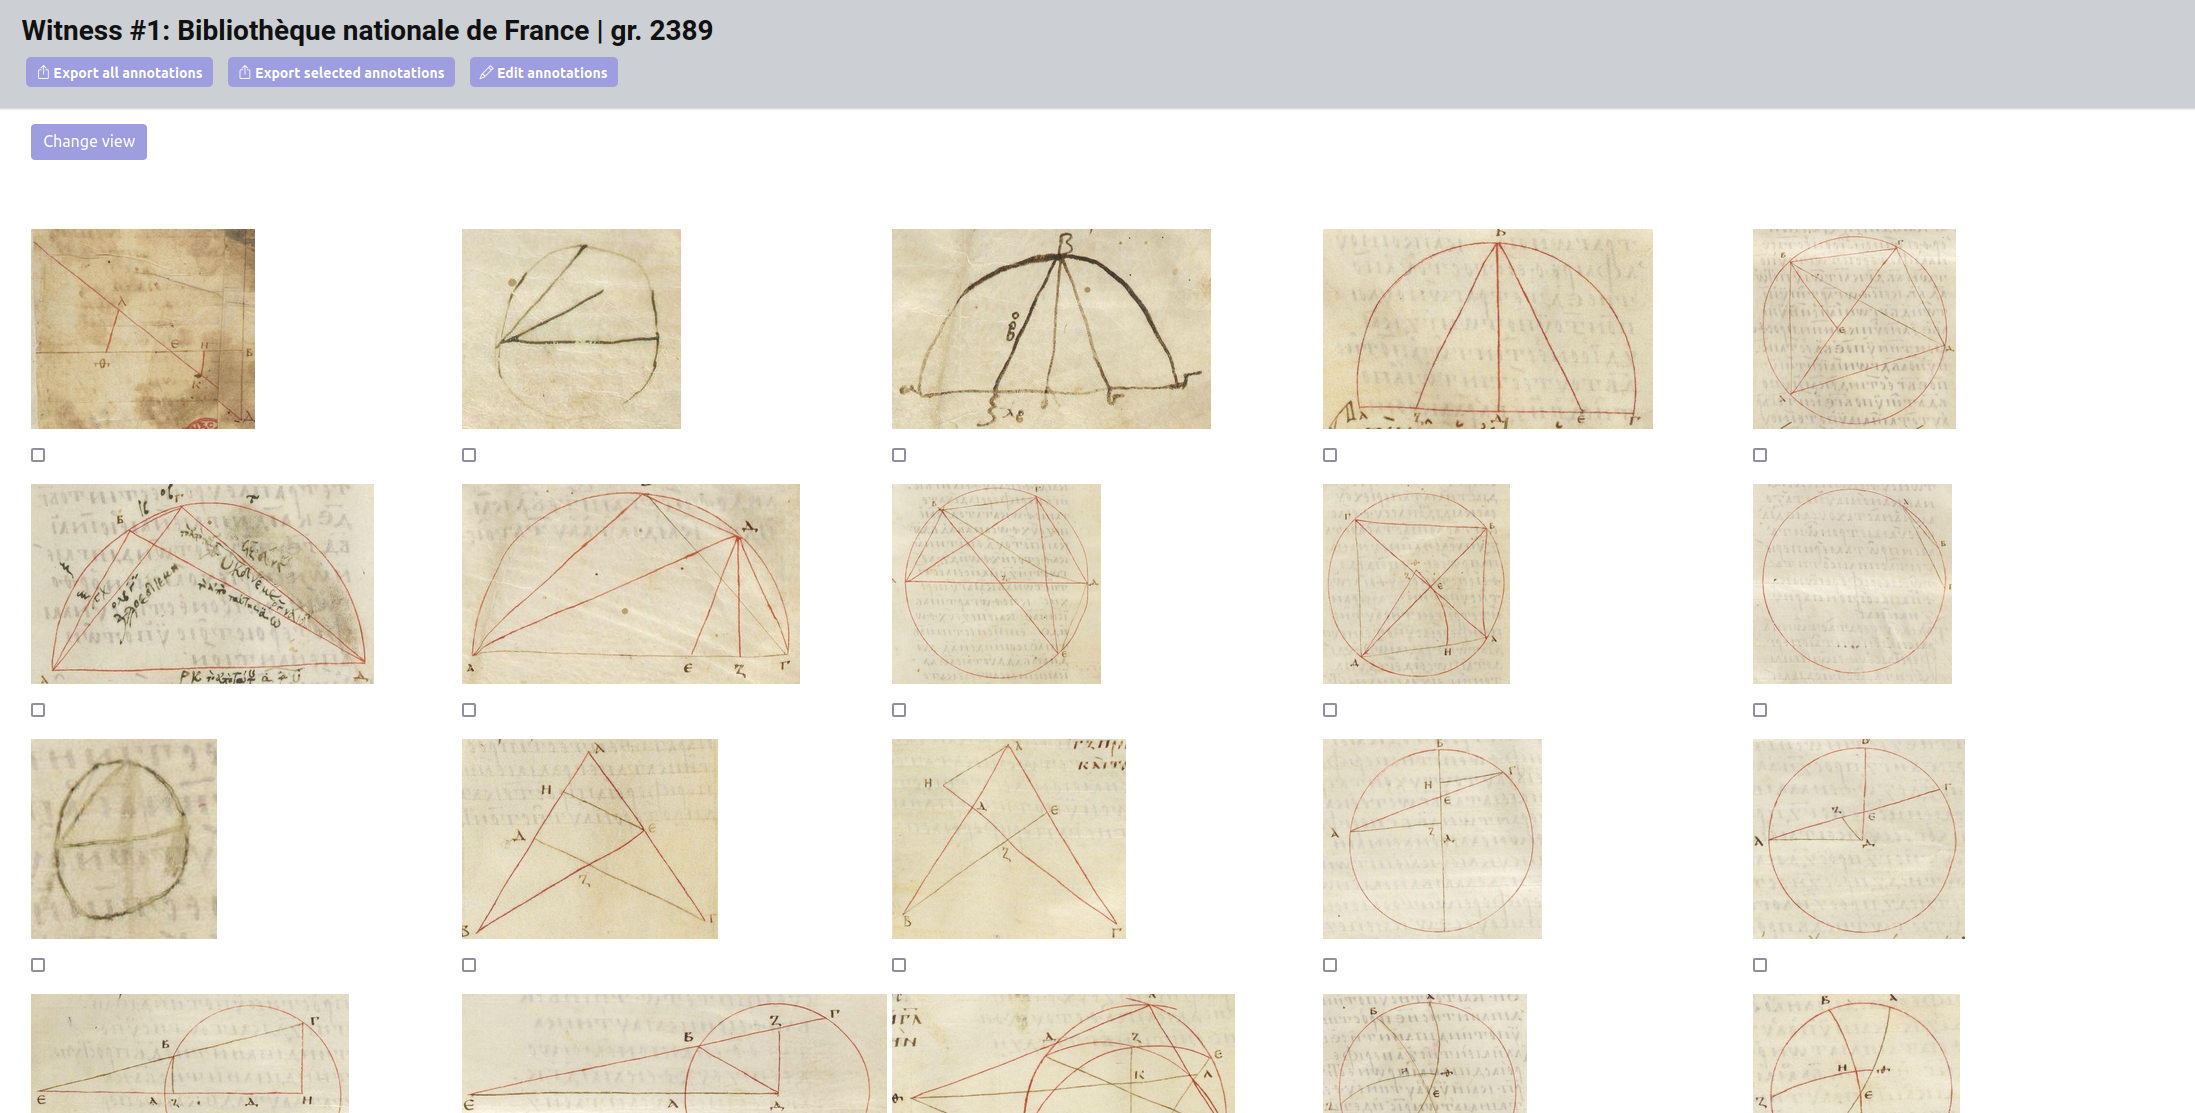
\includegraphics[height=7cm]{figues/vue_dump.png}
          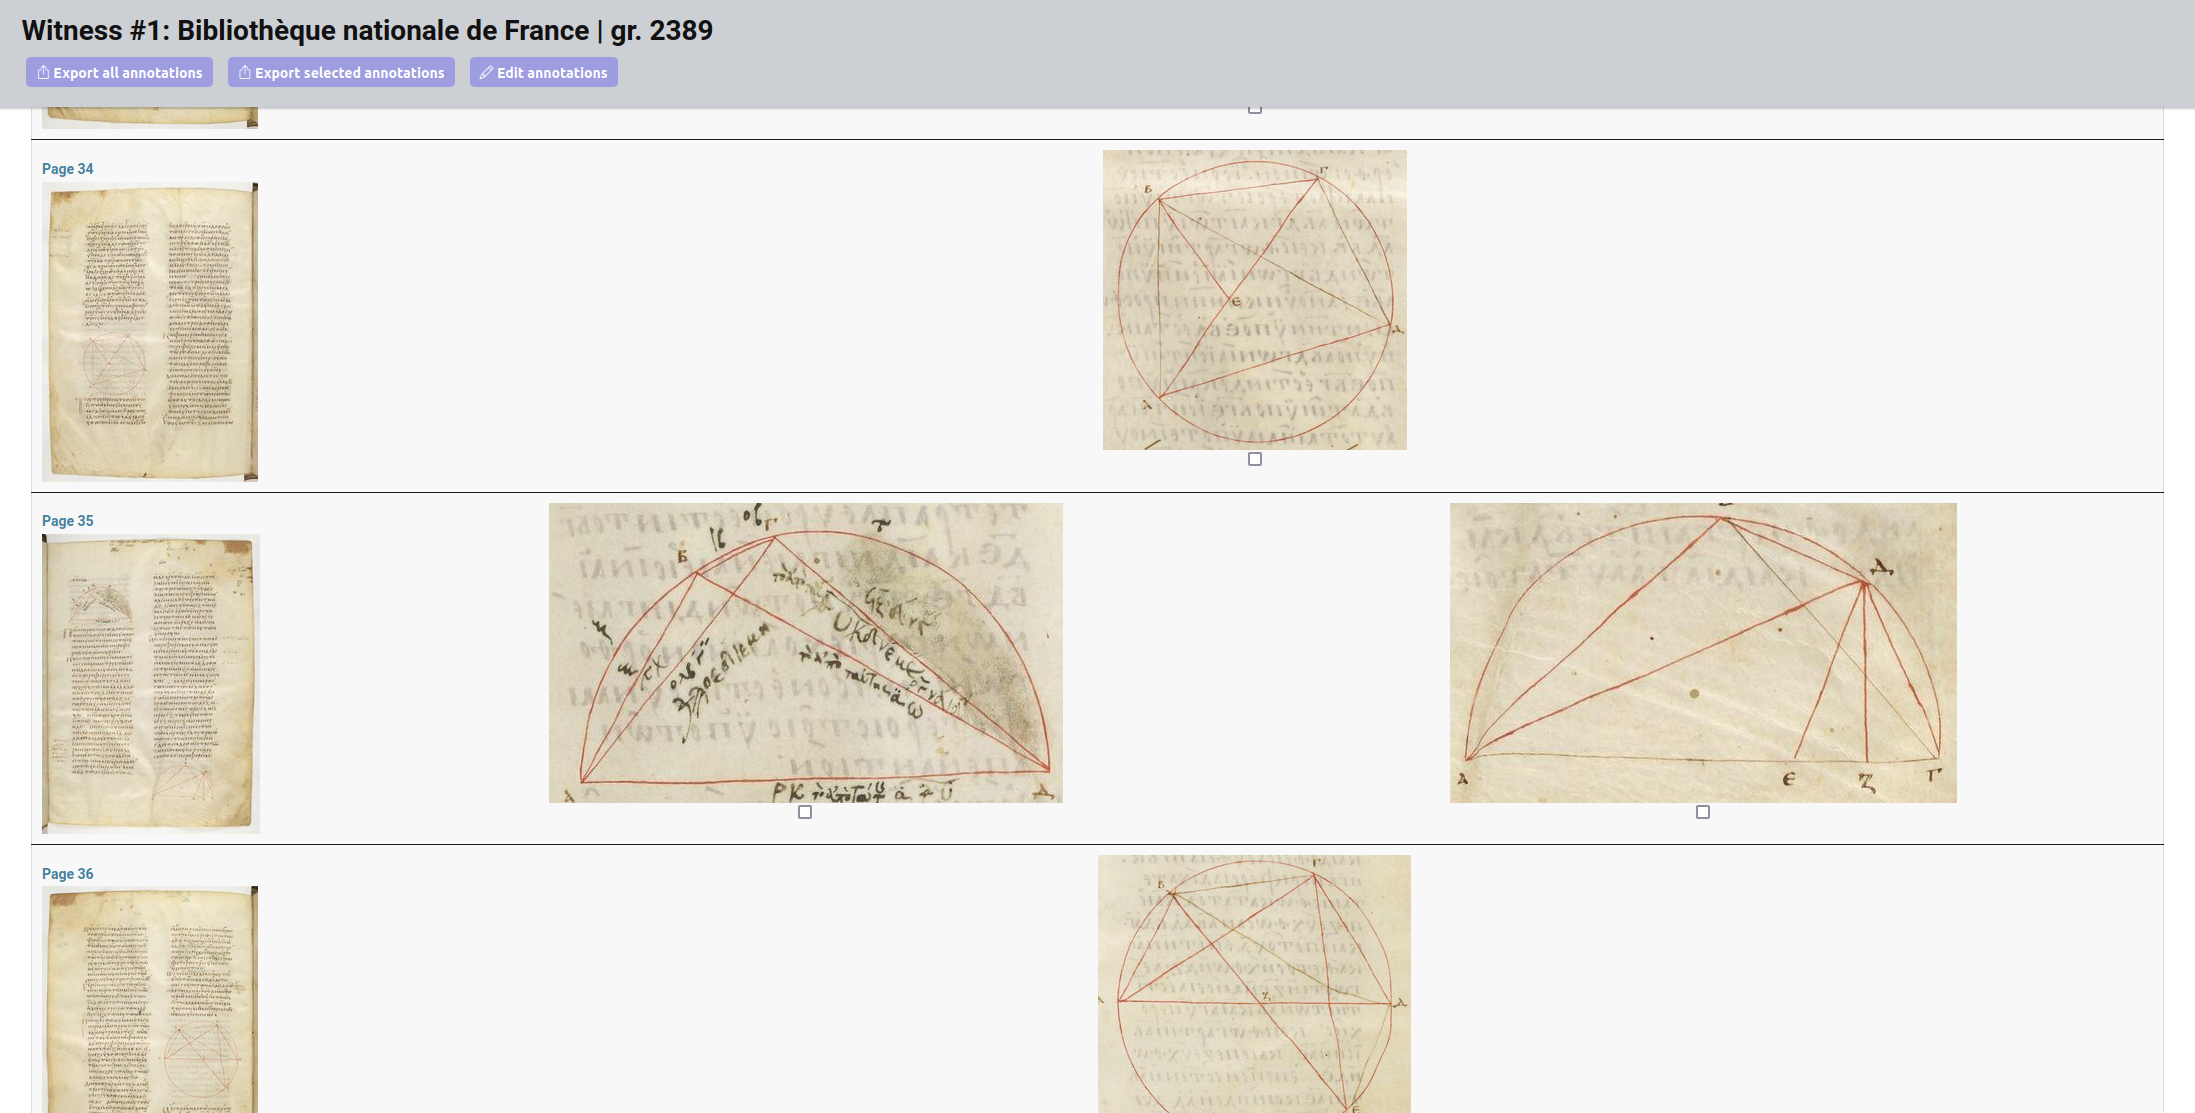
\includegraphics[height=7cm]{figues/vue_contexte.png}
          \end{center}
          \caption{Affichage des extractions, vue \emph{dump} et avec la page de manuscrit en regard.}
          \label{fig:old_interface_1} \end{figure}

Des vues similaires ont été créées pour afficher les résultats de la vectorisation. 

\section{Autres développements }

Vues pour l'export des \svgs et des images \jpeg~: 

\begin{lstlisting}[language=python, frame=single, breaklines=true, caption={Vue pour l'export de tous les \svgs et des images associées.}]

@login_required(login_url=f"/{APP_NAME}-admin/login/")
def export_all_images_and_svgs(request, anno_ref):
    passed, anno = check_ref(anno_ref, "Annotation")
    if not passed:
        return JsonResponse(anno)

    if not ENV("DEBUG"):
        credentials(f"{SAS_APP_URL}/", ENV("SAS_USERNAME"), ENV("SAS_PASSWORD"))

    urls_list = []
    path_list = []

    _, all_annos = formatted_annotations(anno)
    all_crops = [
        (canvas_nb, coord, img_file)
        for canvas_nb, coord, img_file in all_annos
        if coord
    ]

    for canvas_nb, coord, img_file in all_crops:
        urls_list.extend(gen_iiif_url(img_file, 2, f"{c[0]}/full/0") for c in coord)
        vecto_path = f"{img_file[:-4]}_{''.join(c[0] for c in coord)}.svg"
        # Vérifie si le chemin existe
        if os.path.exists(os.path.join(SVG_PATH, vecto_path)):
            path_list.append(vecto_path)

    return zip_images_and_files(urls_list, path_list)

\end{lstlisting}

\begin{lstlisting}[language=python, frame=single, breaklines=true, caption={Vue pour l'export des \svgs et des images \jpeg sélectionnés.}]
@login_required(login_url=f"/{APP_NAME}-admin/login/")
def export_selected_imgs_and_svgs(request):
    images_list = json.loads(request.POST.get("liste_images"))
    urls_list = []
    paths_list = []
    for element in images_list:
        if is_url(element):
            urls_list.append(element)
        else:
            paths_list.append(element)
    return zip_images_and_files(urls_list, paths_list)
\end{lstlisting}

Des fonctions utilitaires sont utiles pour assurer l'export~: 

\begin{lstlisting}[language=python, frame=single, breaklines=true, caption={Fonctions utilitaires pour compresser et télécharger les images.}]

def zip_img(img_list, zip_name=f"{APP_NAME}_export"):
    buffer = io.BytesIO()
    with zipfile.ZipFile(buffer, "w") as z:
        for img_path in img_list:
            img_name = f"{url_to_name(img_path)}.jpg"
            if urlparse(img_path).scheme == "":
                z.write(f"{IMG_PATH}/{img_name}", img_name)
            else:
                response = requests.get(img_path)
                if response.status_code == 200:
                    z.writestr(img_name, response.content)
                else:
                    log(f"[zip_img] Fail to download img: {img_path}")
                    pass

    response = HttpResponse(
        buffer.getvalue(), content_type="application/x-zip-compressed"
    )
    response["Content-Disposition"] = f"attachment; filename={zip_name}.zip"
    return response


def zip_files(filenames_contents, zip_name=f"{APP_NAME}_export"):
    # filenames_contents = [(filename1, content1), (filename2, content2), ...]
    buffer = io.BytesIO()
    with zipfile.ZipFile(buffer, "w") as z:
        for filename_content in filenames_contents:
            filename, content = filename_content
            z.writestr(filename, content)

    response = HttpResponse(
        buffer.getvalue(), content_type="application/x-zip-compressed"
    )
    response["Content-Disposition"] = f"attachment; filename={zip_name}.zip"
    return response


def zip_images_and_files(img_list, file_list, zip_name=f"{APP_NAME}_export"):
    buffer = io.BytesIO()
    with zipfile.ZipFile(buffer, "w") as z:
        # Ajouter des images à partir des URLs ou du répertoire local
        for img_path in img_list:
            img_name = f"{url_to_name(img_path)}.jpg"
            if urlparse(img_path).scheme == "":
                try:
                    z.write(f"{SVG_PATH}/{img_name}", img_name)
                except FileNotFoundError:
                    log(f"[zip_images_and_files] Local image not found: {img_path}")
            else:
                response = requests.get(img_path)
                if response.status_code == 200:
                    z.writestr(img_name, response.content)
                else:
                    log(f"[zip_images_and_files] Fail to download image: {img_path}")

        # Ajouter des fichiers à partir du répertoire mediafiles
        for file_path in file_list:
            try:
                with open(f"{SVG_PATH}/{file_path}", "rb") as f:
                    z.writestr(file_path, f.read())
            except FileNotFoundError:
                log(f"[zip_images_and_files] Local file not found: {file_path}")

    response = HttpResponse(
        buffer.getvalue(), content_type="application/x-zip-compressed"
    )
    response["Content-Disposition"] = f"attachment; filename={zip_name}.zip"
    return response

\end{lstlisting}

\textit{Template} pour afficher les \textit{crops} de diagrammes avec les vectorisations associées. Le \textit{template} et le rendu sont très similaire à ceux concernant l'affichage des diagrammes uniquement~: 

\begin{lstlisting}[language=HTML5, frame=single, breaklines=true, caption={Template \html pour afficher les extractions et leurs vectorisations.}]





{{ anno }}


    <div class="toolbar">
        <div class="title">
            <b>{{ anno|capfirst }}</b>
        </div>
        <div style="display: flex; flex-direction: row;">
            <a href="" target="_blank">
                <button class="export-button" type="submit">
                    <i class="fa-solid fa-eye"></i>
                    
                        Visualize all
                    
                        Voir toutes les
                    
                    annotations
                </button>
            </a>
            <a href="">
                <button class="export-button" type="submit">
                    <i class="fa-regular fa-file-zipper"></i>&nbsp;
                    
                        Download all
                    
                        Télécharger toutes les
                    
                    vectorisations
                </button>
            </a>

            <form id="export" action="" method="post">
                
                <input type="hidden" id="liste_images" name="liste_images" value="">
                <button class="export-button" type="submit">
                    <i class="fa-regular fa-file-zipper"></i>&nbsp;
                    
                        Download selected annotations
                    
                        Télécharger les vectorisations sélectionnées
                    
                </button>
            </form>
        </div>
    </div>




<div class="tabs-crops">
    <div class="row">
        <div class="tab-buttons">
            <button class="btn-change active-tab">
                Page view
            
                Vue page
            
            </button>
            <button class="btn-change">
                Dump view
            
                Vue générale
            
            </button>
        </div>
    </div>


<div class="tab-bodies">

    <div class="row" style="display:block;">
        <div class="column">
            <table class="anno-table" style="margin-top: 0em;">
                
                    <tr class="anno-row">
                        <td class="anno-td page-col">
                            <a href="{{ img_file|img_to_iiif}}" target="_blank">
                                <img class="page-preview" src="{{ img_file|img_to_iiif:"full/350,/0" }}" alt="Click to see real size image">
                            </a>
                            <h3><a href="{{ img_file|img_to_iiif }}" target="_blank">Page {{ canvas_nb }}</a></h3>
                        </td>
                        <td class="anno-td anno-col">
                            
                                <div id="ill_{{ id }}" class="anno-div grid-item" style=" display: flex; flex-wrap: wrap; justify-content: center;">
                                    
                                        <a href="{{ img_file|img_to_iiif:region_full }}" target="_blank">
                                            <img src="{{ img_file|img_to_iiif:region }}" alt="scan preview">
                                        </a>
                                        <img src="svg/{{ img_file|jpg_to_none }}_{{ coords }}.svg" class="img-fluid" alt="{{ img_file|jpg_to_none }}_{{ coords }}.svg">
                                        <a href="" target="_blank">VisualizeVisualiser</a>
                                        <br>
                                        <input type="checkbox" name="vecto_checkbox" value='["{{ img_file|jpg_to_none }}_{{ coords }}.svg", "{{ img_file|img_to_iiif:region }}"]' onchange="updateSelectedImageURLs()">
                                        <label for="checkbox">
                                            SelectSélectionner
                                        </label>
                                    
                                </div>
                            
                        </td>
                    </tr>
                
            </table>
            
        </div>
    </div>

    <div style="display: none;">
        <div style="margin-top: 5%;">
            <div class="grid-container">
                
                    
                        <div class="grid-item">
                            <div style="display: flex; flex-direction: row;">
                                
                                    <a href="{{ img_file|img_to_iiif:small }}" target="_blank">
                                        <img src="{{ img_file|img_to_iiif:small }}" class="img-fluid" alt="{{ img_file }}" style="margin-right: 10px;">
                                    </a>
                                            <img src="svg/{{ img_file|jpg_to_none }}_{{ coords }}.svg" class="img-fluid" alt="{{ img_file|jpg_to_none }}_{{ coords }}.svg">
                                            <a href="{ % url 'img-and-svg' img_file=img_file coords=coords %}" target="_blank">VisualizeVisualiser</a>
                                </a>
                                <input type="checkbox" name="vecto_checkbox" value='["{{ img_file|jpg_to_none }}_{{ coords }}.svg", "{{ img_file|img_to_iiif:small }}"]' onchange="updateSelectedImageURLs()">
                                
                            </div>
                            <h3><a href="{{ img_file|img_to_iiif }}" target="_blank">Page {{ canvas_nb }}</a></h3>
                        </div>
                    
                
            </div>
        </div>
    =</div>

</div>
</div>


<script>
    document.addEventListener('DOMContentLoaded', () => {
        const tabContainers = document.querySelectorAll('.tabs-crops');

        tabContainers.forEach((tabContainer, tabID) => {
            const registerButtons = tabContainer.querySelectorAll('.tab-buttons .btn-change');
            const tabBodies = tabContainer.querySelectorAll('.tab-bodies > div');

            registerButtons.forEach((button, index) => {
                button.setAttribute('aria-controls', `${tabID}_${index}`);
                if (tabBodies[index]) {
                    tabBodies[index].setAttribute('id', `${tabID}_${index}`);
                }

                button.addEventListener('click', () => {
                    setActiveTab(registerButtons, tabBodies, button);
                });
            });
        });

        function setActiveTab(registerButtons, tabBodies, activeButton) {
            registerButtons.forEach((button, index) => {
                if (button === activeButton) {
                    button.classList.add('active-tab');
                    if (tabBodies[index]) {
                        tabBodies[index].style.display = 'block';
                    }
                } else {
                    button.classList.remove('active-tab');
                    if (tabBodies[index]) {
                        tabBodies[index].style.display = 'none';
                    }
                }
                button.setAttribute('aria-expanded', button === activeButton~? 'true'~: 'false');
            });
        }
    });

    var checkboxes = document.querySelectorAll('input[name="vecto_checkbox"]');
    var selectedImages = [];

    function updateSelectedImageURLs() {
    // Clear the selectedImages array before processing checkboxes
    selectedImages.length = 0; // More efficient way to clear the array

    // Loop through all checkboxes
    checkboxes.forEach(function(checkbox) {
        if (checkbox.checked) {
        try {
            // Parse the JSON string from checkbox value (handle potential errors)
            var parsedImages = JSON.parse(checkbox.value);
            // Add parsed images to selectedImages array (assuming correct format)
            selectedImages.push(...parsedImages);
        } catch (error) {
            console.error("Error parsing JSON from checkbox:", checkbox.value, error);
        }
        }
    });

    // Convert the selectedImages array to JSON string (handle empty array)
    var jsonString = selectedImages.length > 0~? JSON.stringify(selectedImages)~: "";

    // Update the hidden input "liste_images" with the JSON string
    document.getElementById("liste_images").value = jsonString;

    // Log the JSON string for verification (optional)
    console.log(selectedImages);
    console.log(jsonString);
    }

    </script>


\end{lstlisting}

\section{Manipuler le format SVG}

Le stage m'a également permis de me familiariser avec le format \svg. J'ai développé une interface basique permettant de manipuler des fichiers \svgs, en implémentant des fonctionnalités de base (Fig. \ref{fig:manip_vecto})~: 
\begin{itemize}
    \item supprimer une primitive (en cliquant dessus)~; 
    \item passer les primitives en noir et blanc~;
    \item \textit{fade} l'image en arrière plan~;
    \item télécharger au format \jpeg l'image et le format vectoriel superposés, et en gardant les modifications effectuées.
\end{itemize}

  \begin{figure}[H]
	\begin{center}
		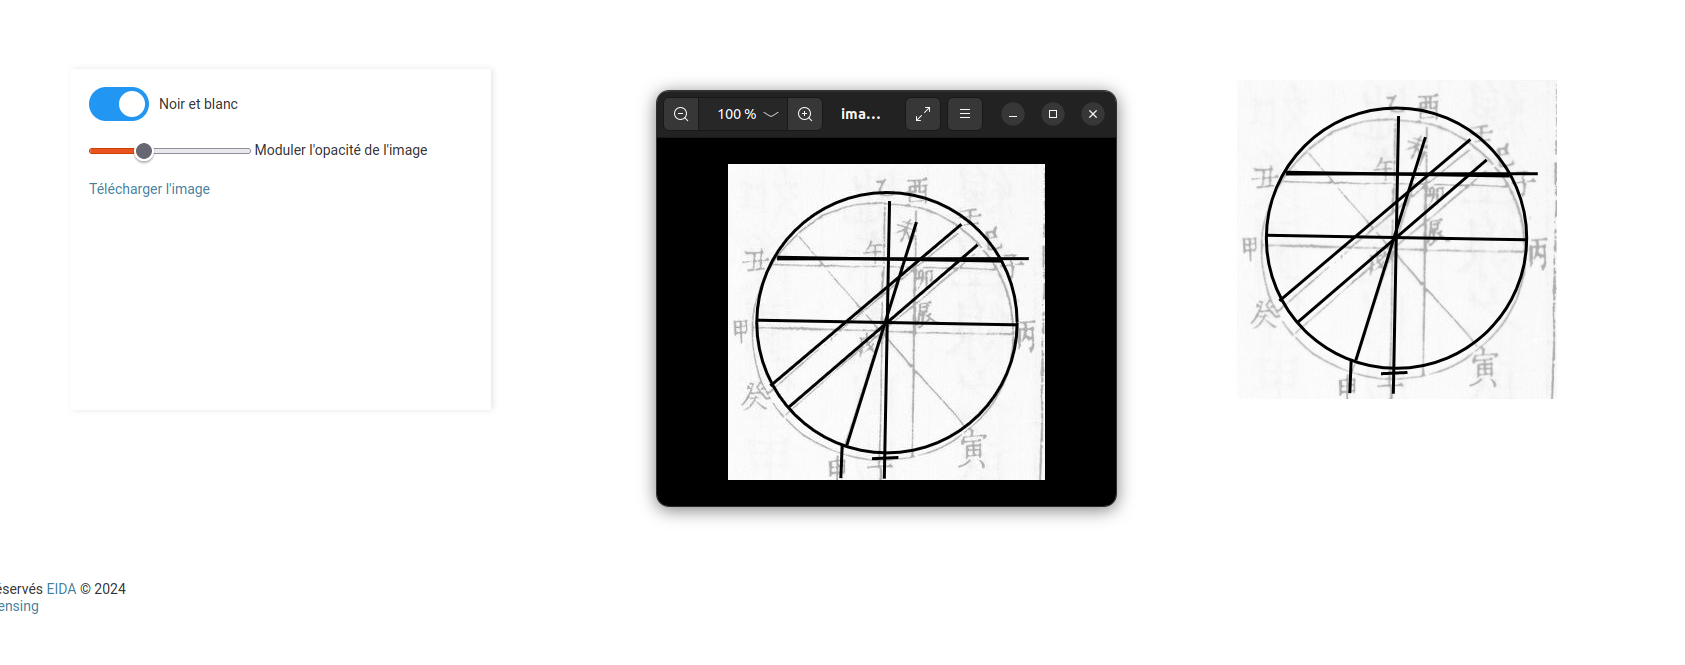
\includegraphics[height=7cm]{figues/manip_vecto.png}
	\end{center}
	\caption{Interface de manipulation des fichiers \svgs, avec exemple d'image modifiée téléchargée.}
	\label{fig:manip_vecto} \end{figure}

J'ai pu ainsi approfondir mes connaissances en JavaScript et découvrir les spécificités du format \svg. La stratégie a consisté à écrire le contenu des fichiers dans le \dom et ajouter de l'interaction grâce à du JavaScript. 

\begin{lstlisting}[language=HTML5, frame=single, breaklines=true, caption={\textit{Template} \html pour la manipulation des fichiers \svgs.}]





{{ regions }}


    {{ block.super }}
    <link rel="stylesheet" href="">
    <link rel="stylesheet" href="">
    <link href="https://cdn.jsdelivr.net/npm/bootstrap-icons@1.8.0/font/bootstrap-icons.css" rel="stylesheet">




    <div class="toolbar">
        <div class="title">
            <b>{{ regions|capfirst }} | page {{ canvas_nb }}</b>
        </div>
    </div>



<div class="container">
    <div class="sidebar">
        <div class="switch-container">
            <label class="switch">
                <input type="checkbox" id="change-stroke-color">
                <span class="slider round"></span>
            </label>
            <label for="change-stroke-color">All lines in blackNoir et blanc</label>
        </div>

        <div>
            <input type="range" min="0" max="1" step="0.01" value="1" id="opacityRange">
            <label for="opacityRange">Toggle Image OpacityModuler l'opacité de l'image</label>
        </div>

        <div>
            <a id="downloadLink" href="#" download="image.jpg">Télécharger l'image</a>
        </div>
    </div>

    <div class="image-container">
        {{ svg_content|safe }}
    </div>
</div>


<script>
    document.addEventListener('DOMContentLoaded', function() {

        const svgElement = document.querySelector('svg'); // Sélectionner l'élément SVG
        const imageElement = document.querySelector('svg image');

        // Charger l'image de fond
        function fond() {
            
            const backgroundImage = "{{ img_file|img_to_iiif:small }}";
            
            imageElement.setAttribute('xlink:href', backgroundImage);
        }
        fond();

        // Changer la couleur des traits
        var toggleSwitch = document.getElementById('change-stroke-color');
        var elementsWithStroke = document.querySelectorAll('[stroke]');
        var originalStrokeColors = [];

        elementsWithStroke.forEach(function(element) {
            originalStrokeColors.push(element.getAttribute('stroke'));
        });

        function changeStrokeColorToBlack() {
            elementsWithStroke.forEach(function(element) {
                element.setAttribute('stroke', 'black');
            });
        }

        function restoreOriginalStrokeColors() {
            elementsWithStroke.forEach(function(element, index) {
                element.setAttribute('stroke', originalStrokeColors[index]);
            });
        }

        toggleSwitch.addEventListener('change', function() {
            if (this.checked) {
                changeStrokeColorToBlack();
            } else {
                restoreOriginalStrokeColors();
            }
        });

        // Modifier l'opacité de l'image
        const opacityRange = document.getElementById("opacityRange");
        opacityRange.addEventListener("input", function() {
            const opacityValue = this.value;
            imageElement.style.opacity = opacityValue;
        });

        // Faire disparaître les éléments onclick
        function removeElementOnClick(event) {
            event.target.remove();
        }

        const circles = document.querySelectorAll('svg circle');
        const paths = document.querySelectorAll('svg path');

        circles.forEach(circle => {
            circle.addEventListener('click', removeElementOnClick);
        });

        paths.forEach(path => {
            path.addEventListener('click', removeElementOnClick);
        });

    // Convertir le SVG modifié en image (PNG ou JPEG)
    function convertModifiedSVGToImage(format, quality, callback) {
        // Sérialiser le SVG modifié
        const svgString = new XMLSerializer().serializeToString(svgElement);

        // Créer un canvas pour dessiner l'image
        const canvas = document.createElement('canvas');
        const context = canvas.getContext('2d');

        // Charger l'image de fond dans le canvas
        const image = new Image();
        image.setAttribute('crossOrigin', 'anonymous');
        image.onload = function() {
            // Le canvas a la même taille que l'image
            canvas.width = image.width;
            canvas.height = image.height;

            // Remplir le canvas avec un fond blanc
            context.fillStyle = 'white';
            context.fillRect(0, 0, canvas.width, canvas.height);

            // Appliquer l'opacité de l'image de fond
            const imageOpacity = parseFloat(window.getComputedStyle(imageElement).opacity);
            context.globalAlpha = isNaN(imageOpacity)~? 1.0~: imageOpacity;
            context.drawImage(image, 0, 0, canvas.width, canvas.height);

            // Réinitialiser l'opacité pour tracer le SVG
            context.globalAlpha = 1.0;

            // Dessiner le SVG modifié sur le canvas
            const svgBlob = new Blob([svgString], { type: 'image/svg+xml;charset=utf-8' });
            const DOMURL = window.URL || window.webkitURL || window;
            const svgUrl = DOMURL.createObjectURL(svgBlob);

            const svgImage = new Image();
            svgImage.onload = function() {
                // Dessiner le SVG à la bonne taille
                context.drawImage(svgImage, 0, 0, canvas.width, canvas.height);

                // Télécharger l'image convertie au format spécifié
                const dataUrl = canvas.toDataURL(`image/${format}`, quality);
                callback(dataUrl); // Utiliser le callback pour manipuler le dataUrl
            };
            svgImage.src = svgUrl;
        };
        image.src = imageElement.getAttribute('xlink:href');
    }

    // Fonction de téléchargement
    function downloadImage(format, quality) {
        convertModifiedSVGToImage(format, quality, function(dataUrl) {
            const downloadLink = document.createElement('a');
            downloadLink.href = dataUrl;
            downloadLink.setAttribute('download', `image.${format}`);
            document.body.appendChild(downloadLink);
            downloadLink.click();
            document.body.removeChild(downloadLink);
        });
    }

    // Lien pour télécharger en JPEG
    const downloadLink = document.getElementById('downloadLink');
    downloadLink.addEventListener('click', function(event) {
        event.preventDefault();
        downloadImage('jpeg', 0.8);
    });

    });
    </script>




\end{lstlisting}

Cette interface est associée à une vue qui renvoie au \textit{template} les informations nécessaires, notamment le contenu du fichier \svg. 

\begin{lstlisting}[language=python, frame=single, breaklines=true, caption={Vue pour relier les données à leur affichage dans l'interface de manipulation.}]
@login_required
def show_crop_vectorization(request, img_file, coords, regions, canvas_nb):
    svg_filename = f"{jpg_to_none(img_file)}_{coords}.svg"
    svg_path = os.path.join(SVG_PATH, svg_filename)

    if not os.path.exists(svg_path):
        print(f"File {svg_path} not found")

    with open(svg_path, "r", encoding="utf-8") as file:
        svg_content = file.read()

    return render(
        request,
        "crop_vecto.html",
        context={
            "img_file": img_file,
            "coords": coords,
            "svg_content": svg_content,
            "regions": regions,
            "canvas_nb": canvas_nb,
        },
    )
\end{lstlisting}

\section{Nouvelles interfaces}

Avec la refonte des interfaces effectuée par les développeuses du projet, ces codes ne sont actuellement plus utilisés dans l'application \aikon, l'utilisation d'un \textit{framework front-end} ayant totalement changé les logiques d'affichage. J'ai cependant eu l'opportunité de poser fondations de la page d'accueil de la plateforme (Fig. \ref{fig:acceuil})~: 

	\begin{figure}[H]
	\begin{center}
		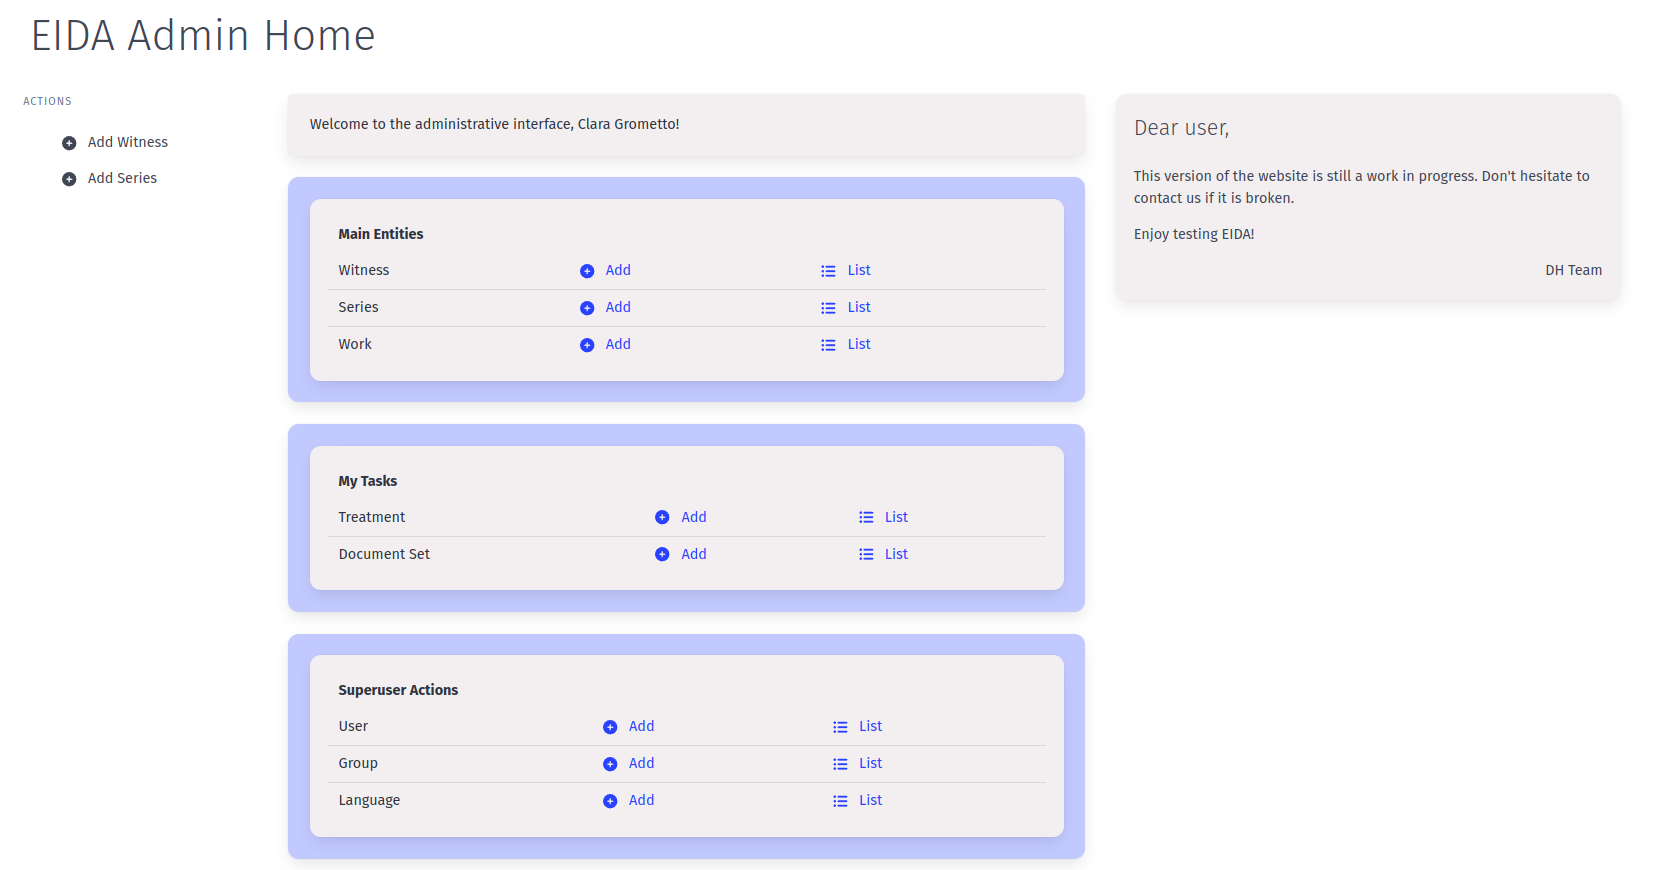
\includegraphics[height=8cm]{figues/accueil.png}
	\end{center}
	\caption{Page d'accueil de la plateforme \aikon}
	\label{fig:accueil} \end{figure}
	\clearemptydoublepage
	
	\chapter[Interfaces~: documentation]{\label{doc_interfaces}Nouvelles interfaces~: documentation}
	\includepdf[scale=1,pages=1-]{templates/annexes/doc_interfaces.pdf}
	\clearemptydoublepage

\clearemptydoublepage

\backmatter
    \printacronyms[title=Liste des acronymes,toctitle=Acronymes, type=\acronymtype]
    \printglossary 
  \listoffigures
  \addtocontents{lof}{\protect\footnotetext{Les schémas suivis d'un astérisque sont prélevés ou inspirés de la documentation technique interne créée par les développeur.ses du projet \eida et de l'\iscd.}}
    \tableofcontents
	
\end{document}